%!TeX spellcheck = en-US
%!TEX root = main.tex
\documentclass[a4paper, 12pt, fourier, numbered, twoside]{PhDThesisPSnPDF}

\ifsetCustomMargin
  \RequirePackage[left=37mm,right=30mm,top=35mm,bottom=30mm]{geometry}
  \setFancyHdr % To apply fancy header after geometry package is loaded
\fi

% *************************** Bibliography  and References ********************

% changes the default name `Bibliography` -> `References'
\usepackage{natbib}
\renewcommand{\bibname}{Bibliography}

% ******************** Captions and Hyperreferencing / URL **********************

\usepackage{color}
\usepackage{hyperref}
\hypersetup{
     colorlinks   = true,
     linkcolor    = blue,
     citecolor    = blue
}

\RequirePackage[labelsep=endash, labelfont=bf, tableposition=above, figureposition=bottom]{caption}

% *************************** Graphics and figures *****************************

\usepackage{rotating}
\usepackage{graphicx}
\usepackage{caption}
\usepackage[position=b]{subcaption}
\captionsetup[subfigure]{width=0.9\textwidth}

% ********************************** Tables ************************************

\usepackage{booktabs} % For professional looking tables
\usepackage{multirow}
\usepackage{tabularx}

% ***************************** Math and SI Units ******************************

\usepackage{amsfonts}
\usepackage{amsmath}
\usepackage{amssymb}
\usepackage{siunitx} % use this package module for SI units

% ******************************* Custom *********************************

\usepackage{soul} % use this for cross line(many fancier options)
\usepackage{pifont}% http://ctan.org/pkg/pifont
\usepackage{enumitem} % for itermize
\newcommand{\cmark}{\ding{51}}% for a tick
\usepackage{indentfirst}
\newlength\longest
\usepackage{atlasphysics}
\usepackage{lipsum}
\usepackage{lineno}
\usepackage[titletoc]{appendix}
\ddmmyyyydate

\usepackage{xspace}
\newcommand\geant{\textsc{Geant\,4}\xspace}
\newcommand\mokka{\textsc{Mokka}\xspace}
\newcommand\ddhep{\textsc{DD4hep}\xspace}
\newcommand\ilcsoft{\textsc{ILCSoft}\xspace}
\newcommand\cpp{\textsc{C++}\xspace}
\newcommand\marlin{\textsc{Marlin}\xspace}
\newcommand\lcio{\textsc{LCIO}\xspace}
\newcommand\qt{\textsc{Qt}\xspace}

\usepackage[acronym, toc]{glossaries}
\glsdisablehyper

\makeatletter
\renewcommand*\l@figure{\@dottedtocline{1}{1.3em}{3em}}
\makeatother

\renewcommand{\arraystretch}{1.2}

\author{Eldwan Brianne}

%!TEX root = main.tex

\makeglossaries

\newacronym{sm}{SM}{Standard Model}
\newacronym{qed}{QED}{Quantum Electro Dynamics}
\newacronym{qcd}{QCD}{Quantum Chromo Dynamics}
\newacronym{qft}{QFT}{Quantum Field Theory}
\newacronym{susy}{SUSY}{Supersymmetry}
\newacronym{cp}{CP}{Charge Parity}
\newacronym{lhc}{LHC}{Large Hadron Collider}
\newacronym{lep}{LEP}{Large Electron-Positron Collider}
\newacronym{cepc}{CEPC}{Circular Electron Positron Collider}
\newacronym{fcc}{FCC}{Future Circular Collider}
\newacronym{ilc}{ILC}{International Linear Collider}
\newacronym{clic}{CLIC}{Compact Linear Collider}
\newacronym{scrf}{SCRF}{Supra Conducting Radio Frequency}
\newacronym{bds}{BDS}{Beam Delivery System}
\newacronym{sid}{SiD}{Silicon Detector}
\newacronym{ild}{ILD}{International Large Detector}
\newacronym{vtx}{VTX}{Vertex Detector}
\newacronym{sit}{SIT}{Intermediate Silicon Tracker}
\newacronym{ftd}{FTD}{Forward Tracking Detector}
\newacronym{tpc}{TPC}{Time Projection Chamber}
\newacronym{gem}{GEM}{Gas Electron Multiplier}
\newacronym{micromegas}{Micromegas}{Micro-Mesh Gaseous Structure}
\newacronym{ecal}{ECAL}{Electromagnetic Calorimeter}
\newacronym{ahcal}{AHCAL}{Analog Hadron Calorimeter}
\newacronym{rpc}{RPC}{Resistive Plate Chamber}
\newacronym{vbf}{VBF}{Vector-Boson Fusion}
\newacronym{br}{BR}{Branching Ratio}
\newacronym{isr}{ISR}{Initial State Radiation}
\newacronym{pdg}{PDG}{Particle Data Group}
\newacronym{mip}{MIP}{Minimum Ionizing Particle}
\newacronym{pfa}{PFA}{Particle Flow Algorithm}
\newacronym{calice}{CALICE}{Calorimeters for Linear Experiments}
\newacronym{sipm}{SiPM}{Silicon Photo-Multiplier}
\newacronym{apd}{APD}{Avalanche Photo-diode}
\newacronym{pde}{PDE}{Photon Detection Efficiency}
\newacronym{asic}{ASIC}{Application Specific Integrated Chip}
\newacronym{skiroc2}{SKIROC2}{Silikon Kalorimeter Read-Out Chip}
\newacronym{adc}{ADC}{Analog to Digital Converter}
\newacronym{tdc}{TDC}{Time to Digital Converter}
\newacronym{spiroc2b}{SPIROC2B}{SiPM Integrated Read-Out Chip}
\newacronym{dac}{DAC}{Digital to Analog Converter}
\newacronym{led}{LED}{Light Emitting Diode}
\newacronym{cern}{CERN}{Conseil europ\'een pour la recherche nucl\'eaire}
\newacronym{fpga}{FPGA}{Field Programmable Gate Array}
\newacronym{bga}{BGA}{Ball Grid Array}
\newacronym{dqm4hep}{DQM4HEP}{Data Quality Monitoring for High Energy Physics}
\newacronym{sps}{SPS}{Super Proton Synchrotron}
\newacronym{bxid}{BXID}{Bunch Crossing Identification}
\newacronym{fhi}{FHI}{First Hard Interaction}
\newacronym{pfo}{PFO}{Particle Flow Object}


\begin{document}

\onehalfspacing
% \singlespacing

\frontmatter
%%% Title page %%%%%%%
%!TEX root = main.tex
\begin{titlepage}

  \thispagestyle{empty}
  \begin{center}

    % {\huge \bf Study of the time development of hadronic showers in data and simulation with the AHCAL technological prototype for a future linear collider experiment\\}
    {\huge \bf Time development of hadronic showers in a Highly Granular Analog Hadron Calorimeter\\}

    \vspace{3cm}

    {\LARGE \bf Dissertation\\}

    \vspace{0.5cm}
    {\Large
    zur Erlangung des Doktorgrades\\
    an der Fakult\"{a}t f\"ur Mathematik, Informatik und Naturwissenschaften\\
    Fachbereich Physik\\
    der Universit\"{a}t Hamburg\\
    \vspace{2.5cm}
    vorgelegt von\\
    \makeatletter
    \textsc{\@author}\\
    \makeatother
    aus Saint-Malo, Frankreich\\

    \vfill

    Hamburg\\
    2018\\
    }

    \newpage
    \thispagestyle{empty}
    \null
    \vfill
    \begin{tabular}{ll}
      Gutachter/innen der Dissertation: & Prof. Dr. Erika Garutti\\
      & Dr. Katja Kr\"uger\\[3mm]
      Zusammensetzung der Pr\"ufungskommission: & Prof. Dr. Erika Garutti\\
      & Dr. Katja Kr\"uger\\
      & Prof. Dr. Johaness Haller\\
      & Prof. Dr. Gudrid Moortgat-Pick\\
      & Prof. Dr. G\"unter H. W. Sigl\\[3mm]
      Vorsitzende/r der Pr\"ufungskommission: & Prof. Dr. G\"unter H. W. Sigl\\[3mm]
      Datum der Disputation: & 03/07/2018\\[3mm]
      Vorsitzender Fach-Promotionsausschusses PHYSIK: & Prof. Dr. Wolfgang Hansen\\[3mm]
      Leiter des Fachbereichs PHYSIK: & Prof. Dr. Michael Potthoff\\[3mm]
      Dekan der Fakult\"at MIN: & Prof. Dr. Heinrich Graener\\[3mm]
    \end{tabular}

  \end{center}
\end{titlepage}

%%%%%%%%%%%%%%%%%%%%%%

%%% Abstract page %%%%%%%
%!TEX root = main.tex
\cleardoublepage
\phantomsection
\addcontentsline{toc}{chapter}{Abstract}

\thispagestyle{empty}
\begin{center}
{\bf Abstract}
\end{center}

This thesis presents the study of the time development of hadronic showers in a highly granular hadron calorimeter using data collected by the CALICE Analog Hadron Calorimeter (AHCAL) technological prototype at the Super Proton Synchrotron (SPS) at CERN in July 2015 in $\mu^-$, $e^-$ and hadron beams up to 90 GeV.

Highly granular calorimeters are designed based on the concept of Particle Flow Algorithm which aims to measure each individual particles in a jet using the best sub-detector measurement. The Particle Flow approach is a key aspect of the detectors for the International Linear Collider (ILC) which is a future linear lepton collider designed for precision physics studies at a center of mass energy up to 500 GeV.

The CALICE Collaboration is developing highly granular calorimeters for the ILC. The AHCAL is one of the detector concepts based on $30\times30\times3$ mm$^3$ scintillating tiles read out by Silicon Photomultipliers (SiPM). The SiPM signal is processed by an ASIC (SPIROC2b) capable to measure the amplitude and the time of individual calorimeter hits. A second generation technological prototype of the AHCAL is developed to focus on the full scalability of the detector. The prototype used in this thesis is composed of 14 active layers corresponding to 3744 channels inserted into an steel absorber structure of 4 $\lambda_i$ depth. For the first time, a large scale prototype has been operated successfully in various beams.

This analysis concentrates on the timing capabilities of the AHCAL prototype. In a first part, the challenging timing calibration procedure, due to the large amount of channels and features of the front-end, is presented. A timing resolution of 5 ns for muons and 8 ns for electron and pion showers has been achieved. In a second part, this thesis shows the study of the time development of hadron showers with the AHCAL prototype by investigating timing correlations with the hit energy, the hit distance to the shower axis and between layers. The results of the testbeam data have been compared to various simulations.

In the last part of this thesis, a study of the effects of timing cuts on calorimeter response, energy resolution and shower topology is presented using a full GEANT4-based simulation of the International Large Detector (ILD) concept. Using the timing information of individual calorimeter hits has the potential to improve pattern recognition and calorimeter energy resolution.

\newpage
\thispagestyle{empty}
\begin{center}
{\bf Zusammenfassung}
\end{center}
\lipsum[23]

%%%%%%%%%%%%%%%%%%%%%%

%%% Table content page %%%%%%%

\tableofcontents

%%%%%%%%%%%%%%%%%%%%%%

%%% Introduction page %%%%%%%

%\linenumbers
%!TEX root = main.tex
\chapter{Introduction}

The \textit{Large Hadron Collider} (LHC) at CERN is the highest energy particle accelerator ever constructed. It is colliding protons at a center of mass energy up to $\sqrt{s}$ = 14 TeV. In 2012, the LHC discovered the \textit{Higgs boson} with the CMS and ATLAS experiments. This marked the accomplishment of a cornerstone of the \textit{Standard Model} of particle physics.

As seen in the past, a lepton collider experiment would be complementary to the results from the LHC in terms of precision measurements and potential discovery. Several concepts of future linear collider experiments exist, the \textit{International Linear Collider} (ILC) and the \textit{Compact Linear Collider} (CLIC). The ILC is planned to collide electrons and positrons at a center of mass energy up to $\sqrt{s}$ = 500 GeV. In order to achieve the best possible measurement precision at the ILC, unprecedented detector resolutions are needed. This can be achieved by the concept of \textit{Particle Flow algorithms}. The detectors are designed based on this approach in order to achieve a jet energy resolution of around 3-4\%. The PFA concept aims to combine measurements of the tracking system and the calorimeters by measuring each individual particles in a jet using the best sub-detector measurement for each particle. This requires calorimeters systems with an unprecedented \textit{granularity}.

Such calorimeter designs also have been selected for the high luminosity upgrade of the LHC. To maintain and improve the current performance of the LHC detectors under the challenging conditions of the HL-LHC, an increase of the longitudinal and lateral segmentation of the calorimeters is needed. While \textit{precision timing measurement} have not been a key aspect in hadron calorimeters, such measurements would allow to identify pile-up jets and would improve the vertex location of di-photon events. A measurement in the order of 20-30 ps (equivalent to around 1 cm separation) would allow the association of energy depositions in the calorimeter with vertices and would significantly reduce fake objects and energy deposits \cite{CMSCollaboration:2015zni}. This is even more important for high rate collision experiments such as CLIC where bunches are separated by 0.5 ns. Moreover, precision timing measurements could act as \textit{software compensation} method. It would improve the calorimeter energy resolution by identifying the different component of a hadronic shower and weighting the calorimeter response accordingly \cite{Benaglia2016}.

This thesis discusses the ongoing development of such highly granular calorimeters within the CALICE collaboration. It focuses on the technological prototype of a scintillator-based hadron calorimeter using Silicon photomultiplier (SiPM) readout designed for a future linear collider experiment. This thesis work is centered on the analysis of testbeam data collected during the summer of 2015 at CERN with the CALICE AHCAL technological prototype.

In Chapter 1, the theoretical foundations for this thesis are summarized. In Chapter 2, the International Linear Collider, the detector concepts and key aspects of the ILC physics program are presented. In Chapter 3, the principles of calorimetry are presented. Furthermore, the concept of Particle Flow Algorithms is explained. The first and second generation calorimeter prototypes within the CALICE collaboration, with a focus on scintillator-SiPM readout, are introduced and compared in Chapter 4. In Chapter 5, the particle shower models in \geant are presented along with the AHCAL simulation model implementation and digitization procedure. The commissioning procedure of the AHCAL technological prototype is introduced and discussed in Chapter 6. In Chapter 7, the testbeam setup for this thesis and event selections are described. The energy scale calibration of the AHCAL is discussed in Chapter 8. In Chapter 9 and 10, the timing analysis of the testbeam data is presented. This analysis includes the timing calibration of the full detector and the validation of the calibration with electron data. In the end, the results of the analysis of pion showers is discussed and compared to several \geant v10.1 physics lists. Finally, in Chapter 11, the effects of timing cuts in the hadronic calorimeter of the full ILD detector simulation are investigated and discussed.


%%%%%%%%%%%%%%%%%%%%%%

%%% Main matter page %%%%%%%
\mainmatter

%% Theory Physics %%%
%!TEX root = ../main.tex
\chapter{Particle Physics: Theory}
\label{chap:Theory}

In this chapter, the theoretical foundations for this thesis are described. A brief overview of the Standard Model of particle physics (\acrshort{sm}) is given in section \ref{sec:SM}. This is followed by a brief description in section \ref{sec:HiggsTheo} of the Higgs mechanism and the particle itself, which is one of the corner of the Standard Model. Finally, open-questions of the Standard Model with possible solutions will be discussed in section \ref{sec:BeyondSM}.

\section{The Standard Model of Particle Physics}
\label{sec:SM}

It is difficult to say when particle physics is born. It has its origins in the discovery of the electron by Thomson \cite{JJThomson:1897} in 1897 and followed by the scattering experiment of Rutherford \cite{Rutherford:1911} in 1909 along with the discovery of radioactivity. This gave rise to the classical model of the atom by Niels Bohr. Following further experiments, it was realized that atoms themselves have an internal structure, and thus leading to the discovery of the nucleons, the proton and the neutron. With energies going higher and higher, more and more particles were discovered. In parallel, a theory that tried to understand radiation and the forces emerged. Finally, it was understood that most of the new discovered particles were composite objects. All sub-atomic particles could be reduced to a small set of \textit{elementary particles} which are known nowadays as the smallest constituents of our universe.

\subsection{The Standard Model framework}

In nature, conservation laws are generally associated with symmetries. This is one fundamental base of particle physics and all interactions between particles can be described by symmetries. The mathematical framework of the Standard Model is the Quantum Field Theory (\acrshort{qft}). The electromagnetic interaction is described by Quantum electrodynamics (\acrshort{qed}), the strong interaction is described by Quantum chromodynamics (\acrshort{qcd}) and the weak interaction is described by the weak theory.

In QFT, each elementary particle is described by a field $\Phi$. To put it simply, a field is a property of space. In QFT, there is no particles, only fields. Particles are a manifestation of the excitation of the fields. The interactions (kinematics and dynamics) of the theory are given by the \textit{Lagrangian density} $\mathcal{L}$ as a function of the field $\Phi(x)$ and its derivatives $\partial_{\mu}\Phi(x)$.

Symmetries are described by requiring the Lagrangian to be invariant under certain transformations. The Standard Model theory is based on gauge group theory and it can be formulated as
\begin{equation}
  SU(3)_{C} \times SU(2)_{L} \times U(1)_{Y}
\end{equation}
where $SU(3)_{C}$ is for QCD and $SU(2)_{L} \times U(1)_{Y}$ for the electroweak theory. The electroweak theory unifies the electromagnetic and weak interactions and is known as the \textit{Glashow-Weinberg-Salam} theory (GWS). These gauge groups are described by the Yang-Mills theory \cite{Yang:1954ek}.

\subsection{Elementary matter particles}

The Standard Model of particle physics is a theory that describes all elementary particles and their interactions. The SM is divided in different classes of elementary matter particles: the \textit{quarks} and the \textit{leptons} otherwise known as \textit{fermions}. All elementary matter particles have a spin of 1/2. Fermions are point-like particles without any internal structure. The interactions between particles are mediated by \textit{gauge bosons} (see section \ref{subsec:Mediators}).

In the Standard Model, there are six \textit{flavors} of quarks and leptons that are divided into three generations according to their masses and their quantum numbers: the \textit{charge} ($Q$), the \textit{spin} ($S$), the \textit{color charge} and the \textit{flavor}. The quarks are divided into two categories: up-type ($u$, $c$, $t$) and down-type quarks ($d$, $s$, $b$) which denote their flavor. Only quarks and gluons (see section \ref{subsec:Mediators}) carry a color charge ($r$, $g$, $b$).

The leptons are divided into charged leptons ($e^-$, $\mu^-$, $\tau^-$) and neutrinos ($\nu_e$, $\nu_{\mu}$, $\nu_{\tau}$). Each lepton has an antiparticle of the same mass and quantum numbers except that they have a opposite sign of charge.

Table \ref{table:Fermions} sums up the fundamental fermions and their properties described in the Standard Model.

\begin{table}[htb!]
  \centering
  \caption{Elementary fermions and their properties in the Standard Model. The masses are from \cite{Patrignani:2016xqp}. The quark masses depend on the calculation scheme.}
  \label{table:Fermions}
  \begin{tabular}{@{}lllll@{}} \toprule
    & \multicolumn{2}{c}{Leptons} & \multicolumn{2}{c}{Quarks} \\ \cmidrule(r){2-5}
    & charged & neutrino & up-type & down-type \\ \midrule
    Charge [$e$] & $\pm$ 1 & 0 & +2/3 & -1/3 \\
    Interact weakly & yes & yes & yes & yes \\
    Interact strongly & no & no & yes & yes \\ \midrule
    1$^{st}$ generation & $e$ (electron) & $v_e$ & $u$ (up) & $d$ (down) \\
    Mass [GeV] & $5.1 \times 10^{-4}$ & $< 2 \times 10^{-9}$ & $\sim 2.2 \times 10^{-3}$ & $\sim 4.7 \times 10^{-3}$\\ \midrule
    2$^{nd}$ generation & $\mu$ (muon) & $v_{\mu}$ & $c$ (charm) & $s$ (strange) \\
    Mass [GeV] & 0.105 & $< 0.19 \times 10^{-3}$ & $\sim$1.28 & $\sim 9.6 \times 10^{-2}$\\ \midrule
    3$^{rd}$ generation & $\tau$ (tau) & $v_{\tau}$ & $t$ (top) & $b$ (bottom) \\
    Mass [GeV] & 1.78 & $< 18.2 \times 10^{-3}$ & $\sim$173.1 & $\sim$4.18\\
    \bottomrule
  \end{tabular}
\end{table}

\subsection{Fundamental Forces and Mediators}
\label{subsec:Mediators}

In the Standard Model, the fundamental forces and interactions are known as:
\begin{itemize}
  \item The \textit{strong force} which is responsible for the interactions of color charged particles.
  \item The \textit{electromagnetic} force which is responsible for the interactions between charged particles.
  \item The \textit{weak force} which is responsible for flavor changing interactions e.g. $\beta$-decay.
  \item The \textit{gravity} which describes interactions between macroscopic and massive objects.
\end{itemize}

Forces are mediated by \textit{gauge bosons} which are a kind of elementary particle of spin 1. The gauge bosons interact with the particles by transferring a discrete amount of energy.

Firstly, the strong force, represented in $SU(3)_{C}$. The mediators of the strong force are 8 massless gluons ($g$) which carry a mixture of color and anti-color charges \cite{Griffiths:343277}.

Secondly, the electromagnetic force is mediated by another massless boson, the photon ($\gamma$).

Thirdly, the weak interaction is mediated by three gauge bosons: the electrically charged $W^+$ and $W^-$ bosons and the neutral $Z^0$ boson. In the Standard Model, the electromagnetic and weak force are unified in the electroweak theory described by the $SU(2)_{L} \times U(1)_{Y}$ symmetry. It is composed of the triplet $W_{\mu}^1, W_{\mu}^2, W_{\mu}^3$ in $SU(2)_{L}$ and a neutral field $B_{\mu}$ in $U(1)$. The mixture of these fields gives rise to the four bosons ($W^{+/-}, Z^0, \gamma$).

Finally, the gravity is not integrated yet into the Standard Model. It appears as the weakest force among all forces and it becomes only relevant for macroscopic objects or at very large distances. It is well described by the \textit{general relativity} theory \cite{Einstein:1905ve} and it is important for astrophysics and cosmology. The gravitational force can be neglected for microscopic objects comparing to the other forces. Table \ref{table:Bosons} sums up the bosons with their properties described in the Standard Model.

\begin{table}[htb!]
  \centering
  \caption{Bosons in the Standard Model. The masses are from \cite{Patrignani:2016xqp}. The photon and gluon are assumed to be massless. Gravitation is not considered}
  \label{table:Bosons}
  \begin{tabular}{@{}lllll@{}} \toprule
    Interaction & Particle & Mass [GeV] & Charge [$e$] & Spin\\
    \midrule
    Strong & $g \times 8$ & 0 & 0 & 1\\
    Electromagnetic & $\gamma$ & 0 & 0 & 1\\
    \multirow{2}{*}{Weak} & $W^{+/-}$ & 80.385 $\pm$ 0.015 & $\pm$ 1 & \multirow{2}{*}{1}\\
    & $Z^0$ & 91.1876 $\pm$ 0.0021 & 0 &\\
    Higgs & $H$ & 125.09 $\pm$ 0.24 & 0 & 0\\
    \bottomrule
  \end{tabular}
\end{table}

The last particle to describe is the Higgs Boson ($H$) which is an elementary particle of spin 0. This boson is one of the cornerstone of the Standard Model. Its properties are shown in table \ref{table:Bosons}.

The principle of gauge invariance (see section \ref{sec:HiggsTheo}) requires that gauge bosons are massless which is fulfilled by the photon and gluon but not by the $W^{+/-}$ and $Z^0$ bosons (see table \ref{table:Bosons}). It means that the electroweak gauge symmetry must be broken to generate masses for the heavy bosons. This is called the \textit{Electroweak Symmetry Breaking} (EWSB) mechanism. It gives rise to the \textit{Higgs mechanism}, which allows all other massive elementary particles to interact with the Higgs field to acquire mass. This mechanism is explained in section \ref{subsec:HiggsMecha}.

The Higgs theory \cite{Higgs:1964pj, Englert:1964et} has been formalized by P. Higgs, F. Englert and R. Brout$^\dagger$\footnote{Diseased in 2011} in 1964. The predicted Higgs particle has been discovered in 2012 at the Large Hadron Collider \cite{Aad:2012tfa, Chatrchyan:2012xdj} with a mass of about 125 GeV and is compatible with the Standard Model.

\section{The Higgs Boson}
\label{sec:HiggsTheo}

\subsection{Gauge invariance in the electroweak sector}

In the Standard Model, the Lagrangian $\mathcal{L}_{D}$, also known as the \textit{Dirac Lagrangian}, describes a free particle with a spin of 1/2 such as the electron \cite{Griffiths:343277}
\begin{equation}
  \mathcal{L}_{D} = i(\hbar c)\overline{\rm \Psi}\gamma^{\mu}\partial_{\mu}\Psi - (mc^2)\overline{\rm \Psi}\Psi
\end{equation}
where $\Psi$ a spinor field, $\gamma^{\mu}$ the Dirac $\gamma$-matrices (four matrices) \cite{Peskin:1995ev} and $m$ the mass of the particle. This Lagrangian is invariant under the \textit{global} gauge transformation $\Psi \rightarrow e^{i\theta}\Psi$ with $\theta$ being constant (equivalent to a simple phase rotation). However, it is not invariant under a \textit{local} gauge transformation where the phase factor $\theta$ is a function of space-time $\theta(x)$.

The local gauge invariance can be restored by adding a new vector field $A_{\mu}$ which follows the local gauge transformation $A_{\mu} \rightarrow A_{\mu} + \partial_{\mu}\lambda$ and by changing the partial derivative $\partial_{\mu}$ with the \textit{covariant derivative} $\mathcal{D}_{\mu} = \partial_{\mu} + i\frac{q}{\hbar c}A_{\mu}$. The local gauge invariant Lagrangian for a free particle of spin 1/2 becomes \cite{Griffiths:343277}
\begin{equation}
  \mathcal{L}_{QED} = i(\hbar c)\overline{\rm \Psi}\gamma^{\mu}\mathcal{D}_{\mu}\Psi - (mc^2)\overline{\rm \Psi}\Psi + (q\overline{\rm \Psi}\gamma^{\mu}\Psi)A_{\mu} - \frac{1}{4}F^{\mu\nu}F_{\mu\nu}
\end{equation}
where $F^{\mu\nu} \equiv \partial^{\mu}A^{\nu} - \partial^{\nu}A^{\mu}$ is the field strength tensor. The term $(q\overline{\rm \Psi}\gamma^{\mu}\Psi)A_{\mu}$ describes the interaction between the fermionic spinor field and the new field, which can be identified as the massless photon.

$\mathcal{L}_{QED}$ is invariant under $U(1)$ assuming that the new field is massless ($m_{A} = 0$). Otherwise, a mass term $m_{A}^2A^{\mu}A_{\mu}$ needs to be included, which breaks the local gauge symmetry. Evidences \cite{Lakes:1998mi, Chibisov:1976mm, Williams:1971ms} have shown that the photon is massless, and therefore $\mathcal{L}_{QED}$ describes well the fermions fields interacting with the photon field, known as Quantum Electrodynamics (\acrshort{qed}).

A similar approach was done by \textit{Yang-Mills} for the weak interaction. It requires the Lagrangian to be invariant under $SU(2)_{L}$ local gauge transformation. This is done by changing the partial derivative with the according \textit{covariant derivative} to satisfy local gauge invariance under $SU(2)_{L}$. The resulting Lagrangian is in the form \cite{Griffiths:343277}
\begin{equation}
  \mathcal{L}_{YM} = i(\hbar c)\overline{\rm \Psi}\gamma^{\mu}\mathcal{D}_{\mu}\Psi - (mc^2)\overline{\rm \Psi}\Psi + (q\overline{\rm \Psi}\gamma^{\mu}\mathbf{T}\Psi) \cdot \mathbf{A_{\mu}} - \frac{1}{4}\mathbf{F^{\mu\nu}} \cdot \mathbf{F_{\mu\nu}}, \quad \Psi = \begin{pmatrix} \Psi_1 \\ \Psi_2 \end{pmatrix}
\end{equation}
with $\Psi_1$ and $\Psi_2$ are four-component field spinors, $\mathcal{D}_{\mu} \equiv \partial_{\mu} + i\frac{q}{\hbar c}\mathbf{T} \cdot \mathbf{A_{\mu}}$ is the covariant derivative. $\mathbf{T}$ refers to the Pauli matrices and $\mathbf{A_{\mu}} = (A_{\mu}^1, A_{\mu}^2, A_{\mu}^3)$ is the new gauge field. This Lagrangian satisfies local gauge symmetry in $SU(2)_{L}$ only if the new gauge bosons are massless.

However, experimental evidences \cite{Rubbia:1983pta} show that the weak bosons $W^{+/-}$ and $Z^0$ have large masses (see table \ref{table:Bosons}). Therefore, the local gauge symmetry must be broken to include their mass terms in the Lagrangian $\mathcal{L}_{YM}$. A new concept is needed in order to restore the local gauge symmetry.

\subsection{The Higgs mechanism}
\label{subsec:HiggsMecha}

The electroweak gauge group $SU(2)_{L} \times U(1)_{Y}$ does not allow for fermions and bosons to be massive in order to conserve the local symmetry. A new framework is needed in order to give mass to the $W^{+/-}$ and $Z^0$ bosons while conserving the local gauge symmetry. The electroweak symmetry breaking (EWSB) provides such framework. It postulates that a self-interacting complex scalar field exists (see section \ref{sec:HiggsSM}) predicting a scalar particle known as the Higgs boson.

In the Standard Model, the Lagrangian for a scalar field $\Phi$ of mass $m$ with spin 0 is written as \cite{Griffiths:343277}
\begin{equation}
  \mathcal{L} = \frac{1}{2}(\partial_{\mu}\Phi)^{\dagger}(\partial^{\mu}\Phi) - \frac{1}{2}\left(\frac{mc}{\hbar}\right)^2\Phi^2
\end{equation}
and can be re-written (from classical Lagrangian) as
\begin{equation} \label{eq:HiggsLag}
  \mathcal{L} = \frac{1}{2}(\partial_{\mu}\Phi)^{\dagger}(\partial^{\mu}\Phi) - V(\Phi)
\end{equation}
where $V(\Phi)$ is the potential term. The potential can be written as:
\begin{equation} \label{eq:HiggsPotential}
  \begin{aligned}
    V(\Phi) & = \mu^2(\Phi^*\Phi) + \lambda(\Phi^*\Phi)^2 \\
    & = \mu^2|\Phi|^2 + \lambda|\Phi|^4
  \end{aligned}
\end{equation}
where $\mu$ and $\lambda > 0$ are real constants. If $\mu^2 > 0$, the vacuum is at zero and the Lagrangian is symmetric. It describes a particle of mass $\mu$ with a self-interaction term. However, if $\mu^2 < 0$, this induces that the potential has a non-zero field value of $v = \sqrt{-\mu^2/\lambda}$. To circumvent this, we can introduce a field centered at the vacuum $\eta = \Phi - v$. Rewriting the Lagrangian in this case yields
\begin{equation}
  \mathcal{L} = \frac{1}{2}(\partial_{\mu}\eta)^{\dagger}(\partial^{\mu}\eta) - \lambda v^2\eta^2 + \text{cubic and quadratic terms}
\end{equation}
This Lagrangian describes the kinematics for a scalar particle of mass $m_{\eta} = \sqrt{2\lambda}v$, the Higgs mass. This describes the principle for the Higgs mechanism for an Abelian\footnote{More commonly a commutative group i.e $a \cdot b = b \cdot a$} group ($U(1)$).

\subsection{Interpretation in the SM}
\label{sec:HiggsSM}

It can be generalized to a non-Abelian\footnote{The counterpart of Abelian groups where commutation is not applicable i.e $a \cdot b \neq b \cdot a$} group ($SU(2)_{L} \times U(1)_{Y}$). In $SU(2)$, the Higgs field is a complex doublet defined as
\begin{equation}
\Phi = \begin{pmatrix} \Phi^+ \\ \Phi^0 \end{pmatrix}= \frac{1}{\sqrt{2}} \begin{pmatrix} \Phi_1+i\Phi_2 \\ \Phi_3+i\Phi_4 \end{pmatrix}
\end{equation}
where $\Phi^+$ is the charged complex component and $\Phi^0$ the neutral component. Following the mechanism explain in section \ref{subsec:HiggsMecha}, if $\mu^2 < 0$ in equation \ref{eq:HiggsPotential}, the symmetry is spontaneously broken such as the neutral component of the Higgs field take a non-zero vacuum expectation value. At the ground state, the Higgs field is of the form
\begin{equation}
\Phi_0 = \frac{1}{\sqrt{2}}\begin{pmatrix} 0 \\ v \end{pmatrix}
\end{equation}
The breaking of the symmetry "eats" three of the four component of the Higgs field.

The Higgs Lagrangian is then becoming
\begin{equation}
  \mathcal{L}_{Higgs} = \underbrace{\frac{1}{2}(\mathcal{D}_{\mu}\Phi)^{\dagger}(\mathcal{D}^{\mu}\Phi)}_{\text{Gauge boson mass term}} - \underbrace{V(\Phi)}_{\text{Higgs mass + self-interaction}}
\end{equation}
where the covariant derivative operator of $SU(2)_{L} \times U(1)_{Y}$ is $\mathcal{D}_{\mu} \equiv \partial_{\mu} + ig\mathbf{T} \cdot \mathbf{W_{\mu}} + ig^{\prime} B_{\mu}Y$ where $g$ and $g^{\prime}$ are the gauge couplings, $\mathbf{W_{\mu}}$ and $B_{\mu}$ are the gauge fields.

This leads to the $W^{+/-}$ and $Z^0$ to acquire mass through interaction with the Higgs such as
\begin{equation}
  \begin{aligned}
    m_{W} &= g\frac{v}{2}\\
    m_{Z} &= \sqrt{g^2 + g^{\prime 2}}\frac{v}{2}
  \end{aligned}
\end{equation}

The couplings of the gauge bosons with the Higgs are proportional to the square of the boson mass given by
\begin{equation}
  g_{HVV} \propto \frac{m_V^2}{v}
\end{equation}

In quantum mechanics, fermions can be left-handed or right-handed (chirality). It is important to make the distinction as the Standard Model treats the chirality differently because only left-handed fermions (right-handed anti-fermions) interact with the W boson. In this case, left-handed fermions are doublets and right-handed are singlets. Right-handed neutrinos have never been observed and are not included here. Both type of fermions interact with the Higgs field and acquire masses through the \textit{Yukawa interactions}. The Yukawa Lagrangian is given by \cite{ILC_TDR_Vol2}
\begin{equation}
  \mathcal{L}_{Yukawa} = - y^u_{ij}\bar{u}_{Ri}\widetilde{\Phi}^{\dagger}Q_{Lj} - y^d_{ij}\bar{d}_{Ri}\Phi^{\dagger}Q_{Lj} - y^l_{ij}\bar{l}_{Ri}\Phi^{\dagger}L_{Lj} + \text{h.c}.
\end{equation}
where $Q_{Lj}$ are left-handed quarks, $\bar{u}_{Ri}$ are right-handed up-type quarks, $\bar{d}_{Ri}$ are right-handed down-type quarks, $L_{Lj}$ are the left-handed leptons and $\bar{l}_{Ri}$ are the right-handed leptons. The term $\widetilde{\Phi} = iT_2\Phi^{*}$ is the Higgs conjugate. The terms $y^u$, $y^d$ and $y^l$ are the Yukawa coupling matrices for up-type quarks, down-type quarks and charged leptons respectively.

All the couplings of fermions with the Higgs can be predicted and are proportional to the fermion mass and $v$ given by
\begin{equation}
  g_{Hff} \propto \frac{m_f}{v}
\end{equation}

The measurement of the Higgs mass is one of the important free parameters of the Standard Model. A precise measurement of the mass is necessary to validate the Standard Model. The Higgs has a large branching ratio, $\sim$58\%, decaying to a pair of bottom quarks. However, in hadron colliders such as the Large Hadron Collider (\acrshort{lhc}), this channel has a very poor signal compared to the background and a poor mass resolution due to large QCD background and thus makes it very challenging for a precise mass measurement.

Lepton colliders (see chapter \ref{chap:FutureColliders}) can offer a precise measurement of the Higgs Boson properties for example by exploiting the $H \rightarrow b\bar{b}$ channel. This implies the measurement of a final hadronic state. The specifics of hadrons are explained in the following section.

\section{Hadron physics}
\label{sec:Hadrons}

Quarks are fundamental particles of the Standard Model govern by the strong interaction. Bound states of quarks forming colorless particles are commonly called \textit{hadrons}. Hadrons are categorized as either \textit{mesons}, which are composed of a pair of quark-antiquark, or \textit{baryons} which are composed of three quarks. The theory of the strong interaction in QFT is known as quantum chromodynamics (QCD). QCD describes the strong interaction under the gauge symmetry group $SU(3)$. Massless bosons known as \textit{gluons} are the mediators of the strong interaction and they can self-interact (on the contrary in QED, the photon has no self-interaction). They carry a mixture of color and anti-color charges creating nine different combinations corresponding to the generators of $SU(3)$.

Quarks have been proven experimentally but no \textit{free} quarks have been observed. This is explained by the \textit{color confinement} in which color charged particles cannot be isolated, and thus quarks cannot be observed directly.

An important aspect of QCD is the \textit{asymptotic freedom}. It means that the strong coupling constant $\alpha_s$ decreases and become small at high energy scales, i.e. at short distances. Asymptotic freedom has the effect that quarks inside a hadron are considered free and not tightly bounded.

In particle physics, experiments observe only hadrons and not quarks. Quarks turn into colorless hadrons through a process called the \textit{hadronization}. This process can only be described phenomenologically. There are three main axioms: the independent hadronization, the string hadronization \cite{Artru1988} and the cluster hadronization \cite{Webber:1983if} but many variant models exist. None of them can be chosen more correct than the other, but they aim to represent the data correctly and to have some predictive power.

In a simple system of a di-jet production in a $e^+e^-$ annihilation, the $q\bar{q}$ partons move away from the common production vertex. The partons are bounded by a \textit{tube} or \textit{string} that confines both objects. At short distances ($<$1 fm), the $q\bar{q}$ pair is considered free. As they are colored particles they can radiate gluons. Since gluons carry color charges, they can also emit radiation. This process is known as \textit{parton showering} \cite{Feynman:1969wa}.

Once the distance become large enough, the energy stored in the string will be sufficient to produce a $q\bar{q}'$ pair. This process continues and creates a cascade of new $q\bar{q}$ pairs until the energy is low enough to hadronize the quarks into colorless hadrons. Unstable hadrons decay further into more stable particles that are observed in the detector. This creates a collimated cascade of particles known as a \textit{jet}.

\section{Beyond the Standard Model}
\label{sec:BeyondSM}

The Standard Model succeeds in describing many experimental results. The current Standard Model is composed of 19 free parameters which are:

\begin{itemize}
  \item The three leptons masses ($m_e$, $m_{\mu}$, $m_{\tau}$)
  \item The six quark masses ($m_u$, $m_d$, $m_c$, $m_s$, $m_b$, $m_t$)
  \item The strong gauge coupling constant $g_s$, the electroweak gauge coupling constants $g$ and $g^{\prime}$
  \item The vacuum expectation value $v$ and the Higgs mass $m_H$
  \item The weak mixing angles ($\theta_{12}$, $\theta_{23}$, $\theta_{13}$) and the CP phase $\delta$ for the flavor-changing weak decays \cite{Kobayashi:1973pt}
\end{itemize}

These parameters have their numerical values determined from experimental data. Nevertheless, there are still open questions that need to be answered, suggesting that the SM is maybe a \textit{low energy} approximation of a higher theory.

\subsection{Open questions of the Standard Model}

\subsubsection*{Gravity}

Gravity is a fundamental force in nature and is explained by the theory of general relativity. The Standard Model does not include gravity and the inclusion of the general relativity into the SM has not been successful so far.

\subsubsection*{Dark Matter}

Astrophysics and Cosmology have given evidences for the existence of invisible matter, e.g. from galaxies observations \cite{Battistelli:2017zrp}, the Cosmological Microwave Background (CMB) \cite{Giesen:2012rp}. This invisible matter is known as the \textit{dark matter}. As these particles have not been found so far, the interaction of dark matter with EM force and strong force have been ruled out. It is supposed that the couplings of dark matter is only through the weak interaction. New physics beyond the Standard Model is needed to explain the nature of these particles.

\subsubsection*{Neutrino masses}

No neutrino masses are present in the Standard Model. As there is no right-handed neutrino, neutrinos cannot acquire mass through Yukawa coupling. However, experiments on neutrino oscillations \cite{Dore:2008dp} shows that neutrinos have a mass. The mechanism by which neutrinos gain mass is so far unclear.

\subsubsection*{Hierarchy problem}

The Higgs mass of around 125 GeV is a theoretical challenge known as the hierarchy problem. In the SM, the mass of the Higgs gets loop corrections from fermion, gauge boson and the Higgs itself \cite{Vieira:2012ex}. If the Standard Model would be valid up to the Plank scale $\Lambda \sim 10^{19}$ GeV, these corrections would make the mass of the Higgs large. To keep the Higgs mass at the electroweak scale $\sim$100 GeV, it would require a very fine-tuning i.e cancellations between the loop corrections and the bare mass. This is considered unnatural.

\subsubsection*{Asymmetry matter-antimatter}

The Standard Model predicts that matter and anti-matter should be in equal amounts in the observable universe. But it is well established that our universe is composed mostly of matter. This \textit{baryon asymmetry} is not explained in the Standard Model. \acrshort{cp} violation \cite{Ellis:1978hq} may be the answer for this asymmetry, it is present in the Standard Model but has only been observed for weak interactions in the quark sector. But the only condition of CP violation would not entirely explain the asymmetry \cite{Sakharov:1967dj}.\\[0.3cm]

Numerous theoreticians are extending the Standard Model to answer few of these questions. One approach is to add symmetries to the Lagrangian. This approach is called \textit{Supersymmetry} (\acrshort{susy}) which adds super-partners to the Standard Model particles differing of a spin of 1/2, i.e. each fermion has a boson super-partner and vice-versa.

\begin{center}
  \rule{0.5\textwidth}{.4pt}
\end{center}

The Standard Model is so far the most reliable theory of the elementary objects and the interactions that govern our world. The Higgs is one of the cornerstone of the theory, therefore, a very precise measurement of its properties such as mass and couplings are needed. This enables us to probe the Standard Model deeply and look for any deviations to the SM predictions that would suggest physics beyond the Standard Model. Measurements at hadrons colliders, like the \acrlong{lhc}, suggest that if any other particle exists, it would be at a multi-TeV scale. However, the effect of such particles on coupling measurements would be below the percent level. Currently, the LHC does not achieve the level of precision needed to distinguish theories beyond the Standard Model \cite{CMS:2013xfa}. A lepton collider would be the perfect tool to conduct precision measurements including the Higgs as shown in chapter \ref{chap:FutureColliders}.


%% ILC description %%%
%!TEX root = ../main.tex
\chapter{Future $e^+e^-$ linear collider experiments}
\label{chap:FutureColliders}

Currently, the only high energy collider in operation is the \textit{Large Hadron Collider} (LHC) at CERN between Switzerland and France. The construction of the LHC started in 1995, was achieved in 2008 and its operation started in 2009. The LHC machine lies in a long underground tunnel of 27 km of circumference and is colliding protons at a center-of-mass energy up to $\sqrt{s} = 14$ TeV using supra-conducting magnets. It is probing the Standard Model to an unprecedented energy scale and search for unknown particles beyond the Standard Model. The discovery of the Higgs Boson in 2012 was one of the major milestone of the LHC. The colliding particles are protons which are composites particles, thus only a fraction of the energy is available during the collision. These collisions are very complex and make some measurements almost impossible at the LHC.

In the past, $e^+e^-$ colliders have been complementary tools to hadron colliders like the \textit{Large Electron-Positron Collider} (LEP) at CERN and Tevatron at Fermilab. A limitation of $e^+e^-$ ring colliders is the maximum achievable collision energy which is limited by the energy losses of the particles due to the synchrotron radiation. The synchrotron radiation power scales as
\begin{equation}
  P_{synchrotron} \propto \frac{E^4}{R \times m^4}
\end{equation}
with $E$ the particle energy, $m$ the mass of the particle and $R$ the accelerator radius. The mass dependence makes the radiation losses significantly higher than protons. The maximum energy achieved by a $e^+e^-$ ring collider was of around a center-of-mass energy of $\sqrt{s} = 210$ GeV with the LEP. In this conditions, around 8 MW of energy is lost by synchrotron radiation.
Therefore, it is most likely that the next $e^+e^-$ collider will be a linear accelerator to achieve energies near the TeV scale.

The \textit{International Linear Collider} (ILC) and The \textit{Compact Linear Collider} (CLIC) are two proposed particle physics accelerator complementary to the LHC. The ILC is designed to collide electrons and positrons at a center-of-mass energy between 250 GeV to 500 GeV with a possible upgrade to 1 TeV. The advantage of the ILC is that it provides a reduced background and cleaner events compared to a hadron collider thus allowing for high precision measurements. The following section will give a short summary of the ILC machine and its detectors and based on the ILC Technical Design Report (TDR) \cite{ILC_TDR_Vol1, ILC_TDR_Vol2, ILC_TDR_Vol3.1, ILC_TDR_Vol3.2, ILC_TDR_Vol4}.

\section{The International Linear Collider}
\label{sec:ILC}

The International Linear Collider (ILC) is a planned 31 km long $e^+e^-$ linear collider to be build in Japan with a design peak luminosity of around $2 \times 10^{34} cm^{-2}s^{-1}$ and a center-of-mass energy of 500 GeV. An upgrade up to 1 TeV center-of-mass energy and a higher luminosity is possible. Polarization up to 80\% for electrons and 30\% for positrons can be achieved enabling the enhancement of rates and the reduction of SM background. The polarization is a crucial ingredient in the ILC program. It uses supra-conductive RF (SCRF) cavities to accelerate electrons and positrons. The project is currently under discussion between the governments and a decision by the end of 2018 should be reached. A schematic of the ILC layout is shown in figure \ref{fig:ILC_schematic}.

\begin{figure}[htbp!]
  \centering
  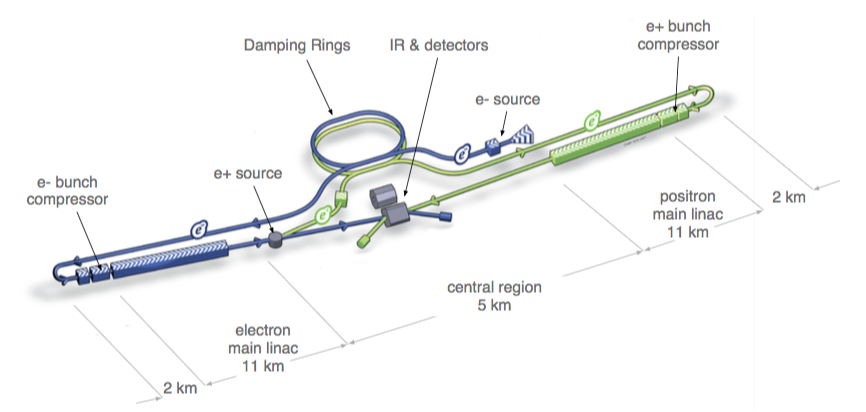
\includegraphics[width=0.7\linewidth]{chap2/fig/ILC_schematic.png}
  \caption{Schematic of the International Linear Collider (not to scale). Taken from \cite{ILC_TDR_Vol1}.} \label{fig:ILC_schematic}
\end{figure}

The electron beam is produced by a laser illuminating a photocathode of GaAs in a DC gun. It provides the bunches of electrons with a polarization of 90\%. The bunches are accelerated to 5 GeV in a SCRF booster before being collected in the dumping ring. The dumping ring has a circumference of 3.2 km where bunch trains are formed and the emittance of the beam reduced by 5 orders of magnitude to 20 nm. It is achieved by the succession of normal magnets, supra-conducting magnets and wiggler magnets. The wiggler magnets cool the beam by dumping synchrotron radiation thus reducing the beam emittance. The bunch trains formed by the ring are around 200 ms apart containing more than 1000 electron bunches.

The electron beam is then transported by the Ring to Main Linac (RTML), accelerating electrons from 5 GeV to 15 GeV while compressing the bunch-length to few micrometers required by the integration region (IR).

The main linacs of the ILC accelerate the electron beam up to 250 GeV by using supra-conductive RF cavities of niobium operated at 2 Kelvins housed in cryomodules. The RF power is delivered by a system of Klystrons. The average gradient of the cavities is around 31.5 $\frac{MV}{m}$ with a quality factor $Q_0 \geqslant 10^{10}$. The synchrotron sources of FLASH and recently of the European X-Ray Free Electron Laser (XFEL) based at DESY, are a demonstration of the mass-production and operation of cryomodules which represents around 1\% of the ILC.

After the acceleration, the electron beam is transported through a supra-conducting helical undulator which generates photons between 10 to 30 MeV. Then the electron beam is separated from the photon beam and transported by the Beam Delivery System (BDS) to the IR. The BDS focuses the beam down to 474 nm $\times$ 5.9 nm (x and y respectively at $\sqrt{s} = 500$ GeV) to reach the luminosity goal of $2 \times 10^{34} cm^{-2}s^{-1}$.

The photons are directed onto a thin ($0.4 X_0$) titanium alloy (Ti) target producing electrons-positrons pairs. The positrons are accelerated to 400 MeV in a first step while the remaining electrons and photons are dumped. The positrons are accelerated to 5 GeV by a booster and injected into a dumping ring, parallel to the electron ring. From there, the positron beam follows a similar beam line as the electron beam and both beams are brought into collision at the IR, where two detectors lie that can be operated in push-pull configuration.

\begin{figure}[htbp!]
  \centering
  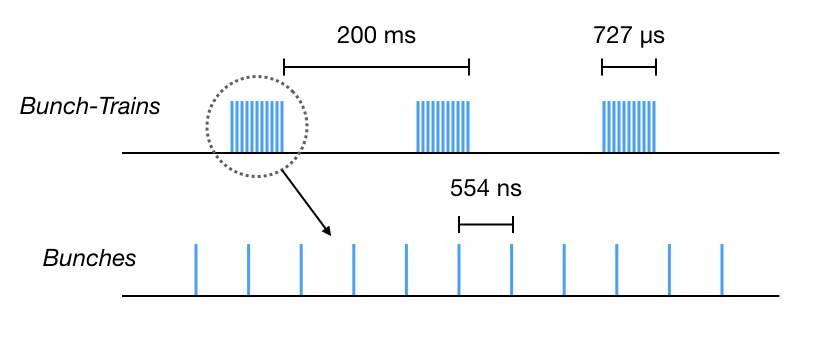
\includegraphics[width=0.7\linewidth]{chap2/fig/BeamStructure.jpeg}
  \caption{Schematic of beam structure of the ILC operated a design parameters.} \label{fig:ILC_BeamStruct}
\end{figure}

The beam structure of the ILC consists of bunch-trains of 1312 bunches of $2 \times 10^{10}$ particles each and separated by around 550 ns. The distance between bunch-trains is around 200 ms corresponding to a 5 Hz repetition frequency (up to 10 Hz depending on the running scenario). A schematic of the beam structure is shown in figure \ref{fig:ILC_BeamStruct}.

The CLIC concept \cite{CLIC_CDR} is drastically different in the design and technology used. CLIC uses normal conducting copper cavities operated at 12 GHz much higher than ILC (1.3 Ghz). It uses a two beam operation scheme where a high current, low energy drive beam provides RF power to accelerate a low current, high energy beam. By this mean, a center-of-mass energy up to $\sqrt{s} = 3$ TeV could be achieved. The CLIC technology is yet not mature compared to the ILC and still needs several years of R\&D before a full CLIC accelerator could be constructed.

\section{The International Large Detector (ILD)}
\label{sec:ILD}

The physics program of the ILC is quite ambitious. In order to realize it, significant advances in detector performance is essential. The detector concepts for the ILC are focused on the \textit{Particle Flow} approach. The Particle Flow approach is discussed in section \ref{sec:PFA}. It is aiming to reconstruct individually each particles in an event. This requires an unprecedented spacial resolution in all sub-detectors to efficiently separate charged and neutral particles even within jets. This motivates for a highly efficient tracking system and highly granular calorimeters but also a sophisticated reconstruction software.

At the ILC, it is planned to have two detector experiments sharing the interaction region in a push-pull configuration. One detector occupies the IR while the other detector is parked in the detector hall. Both detectors can be moved in and out of the IR periodically every few weeks. Two detector concepts have been developed in the ILC Technical Design Report \cite{ILC_TDR_Vol4}, the \textit{Silicon Detector} (SiD) and the \textit{International Large Detector} (ILD). A detailed detector simulation is available for both of the concepts and has been used extensively in the study of the potential of ILC physics as well as detector optimizations. The detectors concepts contain realistic implementations of all sub-detectors and have been cross-checked with prototype data if possible (see chapter \ref{chap:CALICE_Det}). In the following, the ILD detector will be briefly described.

The ILD detector is a multi-purpose detector. The tracking system and the calorimeter systems are both located within a supra-conducting solenoid magnet of 3.4 m radius providing a field of 3.5 T parallel to the beam axis. Schematics of the ILD detector can be seen in figure \ref{fig:ILD}.

\begin{figure}[htbp!]
  \centering
  \begin{subfigure}[t]{0.49\textwidth}
    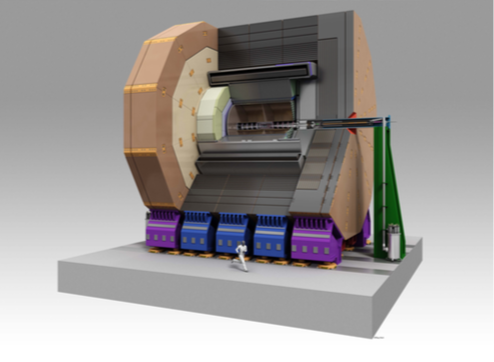
\includegraphics[width=1.\linewidth]{chap2/fig/ILD_full.png}
  \end{subfigure}
  \hfill
  \begin{subfigure}[t]{0.49\textwidth}
    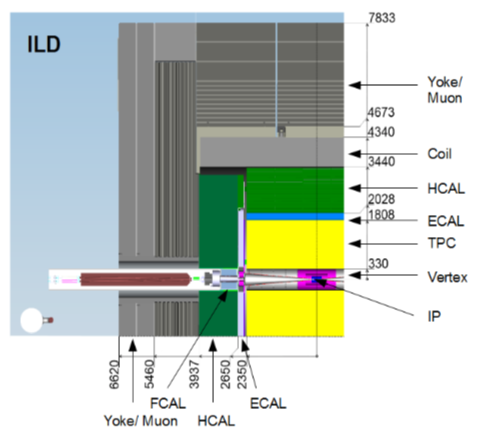
\includegraphics[width=1.\linewidth]{chap2/fig/ILD_layout.png}
  \end{subfigure}
  \caption{Schematic views of the ILD detector. Dimensions on the right figure are in mm. \cite{ILC_TDR_Vol4}.} \label{fig:ILD}
\end{figure}

\subsection{ILD Tracking System}

The ILD Tracking system consists of a multi-layer pixel vertex detector (VTX) at the innermost part, at around 1.6 cm of the beam pipe. Different geometry are proposed, a three double layer or a five single layer silicon pixel geometry. Additionally, two layers of silicon strip detector (SIT) are placed around the vertex detector to close the gap between the VTX and the TPC. In the forward region, silicon pixel disks and silicon strip disks (FTD) are installed to provide coverage at track low angles. The VTX offers position hit resolutions of less than \SI{6}{\micro\meter} with a very low material budget of 0.15\% $X_0$ per layer. The SIT and FTD pixel detectors offers similar position hit resolutions with a material budget of 0.65\% $X_0$. While the technology has not been decided yet, the VTX is optimized for the higher single point resolution and minimum material budget. The high resolution of the VTX offers the best performance for the flavor tagging of jets, even in the very forward direction.

The main feature of the ILD tracking system is a large \textit{Time Projection Chamber} (TPC) providing more than 200 points per track, covering from 330 mm to 1808 mm in radius. The TPC uses the fact that a particle traversing the gas inside the TPC, ionize it along its trajectory. The free electrons are then drifting towards the endcaps (endplates) by an electric field parallel to the beam axis. The endplate detects the ionization electrons by a \textit{Gas Electron Multiplier} (GEM) or a \textit{Micro-Mesh Gaseous Structure} (Micromegas) readout system. The spacial resolution of the TPC is better than \SI{100}{\micro\meter} and also offer a double hit resolution in the order of less than 2 mm. This resolution is worse than silicon tracking can offer but the TPC presents the advantage of a very low material budget, continuous tracking and excellent reconstruction of the non-pointing tracks (Kinks) from multiple scattering. In addition, the TPC offers the possibility of particle identification via the specific energy loss $\frac{dE}{dx}$ (see subsection \ref{subsec:PartInter}).

A combined momentum resolution of $\sigma_{1/p_T} = 2 \times 10^{-5}$ GeV$^{-1}$ has been achieved for high momenta for the ILD tracking system.

\subsection{ILD Calorimeter System}

The ILD calorimeter system is designed and optimized for \textit{Particle Flow} (see section \ref{sec:PFA}). It is aiming to achieve a jet energy resolution $\sigma_E/E$ of around 3-4 \% for the energy range of 45 to 250 GeV. The excellent track reconstruction combined with the calorimeter system requires an unprecedented 3D granularity for the calorimeters to achieve such goals. To minimize material and optimize track associations to depositions in the calorimeters, they are located inside the solenoid magnet thus limiting the depth of the calorimeters. A reasonable trade-off between intrinsic energy resolution and granularity is present in the ILD calorimeter system.

The ILD baseline consists of the electromagnetic calorimeter (ECAL) using silicon based readout with a $5 \times 5$ mm segmentation in a tungsten absorber, allowing a very compact design and the hadronic calorimeter with scintillator-tile based analog readout (AHCAL) with a segmentation of $3 \times 3$ cm in a steel absorber. More details on the AHCAL can be read in chapter \ref{chap:CALICE_Det}. In the forward region, additional calorimeters are placed, LumiCal, BeamCal and LHCAL for luminosity monitoring, beamstralhungs measurement and hermiticity at low angles.

After the solenoid magnet, an iron yoke returns the magnetic field and is planned to be instrumented with scintillator strips or resistive plate chambers (RPCs) to serve as a muon detector and tail catcher for high energy jets.

\section{The SiD Detector}

The SiD detector concept is very similar to the ILD detector. It differs by its size much smaller than ILD, the use of a stronger magnetic field (5 T) and a full silicon tracking system instead of a TPC. The ECAL is the same using silicon as active material. Resistive plate chambers (RPCs) with gas as active material were planned to be used for the hadron calorimeter system but a recent change in the baseline design includes now a scintillator-tile hadronic calorimeter. The performance of SiD is very close in numbers to ILD.

\section{ILC Physics}
\label{sec:ILC_Physics}

The ILC Physics program is very ambitious and complementary to studies done at the LHC. The recent discovery of the Higgs Boson in the 125 GeV range at the LHC which was for several decades the missing block of the SM can be studied with much more precision with the ILC. The probing of the characteristics of the Higgs Boson to a percent level is necessary to validate the current SM but also to be able to observe any deviations to predictions that would be a strong hint for physics beyond the SM. Many other opportunities are provided by the ILC for the study of new physics, the Z and W Bosons and the top quark that can be studied with high precision. This section will describe few key points of the ILC physics program.

\subsection{Higgs Physics}

The ILC experiment provides a precise and model independent measurement of the Higgs Boson characteristics such as its mass, full decay width and absolute coupling to SM particles. The precision on some of theses parameters at LHC is significantly worse than for ILC where a clean, low background environment and well defined initial state is present. The full decay width is not accessible at the LHC in a model independent way thus absolute couplings also.

\subsubsection{Higgs production and decay modes}

There are two main production modes of the Higgs at the ILC, the \textit{Higgsstrahlung} and \textit{Vector Boson Fusion} (VBF). The \textit{Higgsstrahlung} process is the production of a Higgs Boson in association with a Z Boson. For the VBF mode, either two Z or W Bosons fuse in a Higgs Boson in association with either an electron-positron pair or neutrino-antineutrino pair. The Feymann diagrams are shown in figure \ref{fig:HiggsProd}.

\begin{figure}[htbp!]
  \centering
  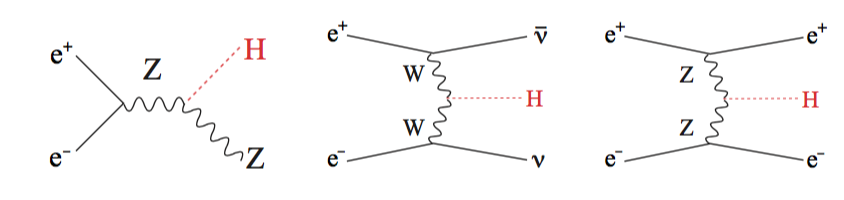
\includegraphics[width=1\linewidth]{chap2/fig/HiggsProd.png}
  \caption{Feymann diagrams for the Higgs production at the ILC at Tree level. \cite{ILC_TDR_Vol2}} \label{fig:HiggsProd}
\end{figure}

At $\sqrt{s}$ = 250 GeV, the Higgsstrahlung process is dominant, the production cross-section peaks at $\sqrt{s}$ = 250 GeV. At higher energies around $\sqrt{s}$ = 450 GeV, the VBF production cross-section starts to dominate. The figure \ref{fig:HiggsXS} shows the evolution of the Higgs production cross-section as function of center-of-mass energy $\sqrt{s}$.
The Higgs decays mostly into a pair of b quarks ($\sim$ 57\%). The next highest branching ratio (BR) is to a $WW^*$ pair ($\sim$ 21\%). Then in the order of few percents, the Higgs decays to $gg$, $ZZ^*$, $\tau \tau$, $cc$. The difference of BR between $h \rightarrow WW^*$ and $h \rightarrow ZZ^*$ is quite interesting with an order of magnitude difference. This explained by the fact that the one of the Z is further off-shell than the one of the W due to $m_h << 2 \times m_W < 2 \times m_Z$ thus suppressing the Z BR.
Other decays to $\mu \mu$, $\gamma \gamma$ and $Z\gamma$ are very rare below 1\%. Massless final states decays are possible through heavy quark loops (top loop). The main branching ratios are depicted in figure \ref{fig:HiggsBR}.

\begin{figure}[htbp!]
  \centering
  \begin{subfigure}[t]{0.49\textwidth}
    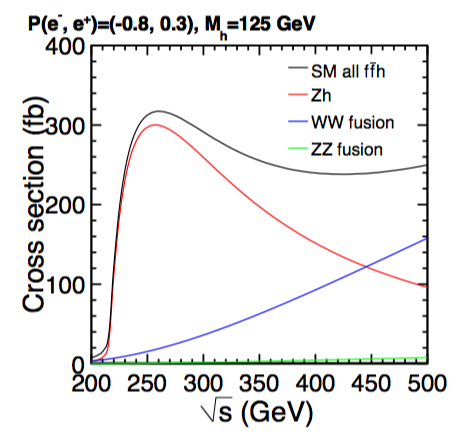
\includegraphics[width=1.\linewidth]{chap2/fig/HiggsXS.png}
    \caption{} \label{fig:HiggsXS}
  \end{subfigure}
  \hfill
  \begin{subfigure}[t]{0.49\textwidth}
    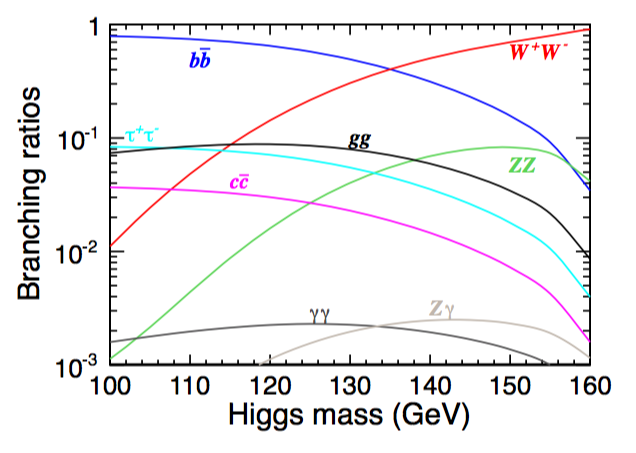
\includegraphics[width=1.\linewidth]{chap2/fig/HiggsBR.png}
    \caption{} \label{fig:HiggsBR}
  \end{subfigure}
  \caption{\subref{fig:HiggsXS}) Production cross-sections for the Higgs at the ILC as function of $\sqrt{s}$. \subref{fig:HiggsBR}) Higgs branching ratios as function of the Higgs mass.}
\end{figure}

\subsubsection{Recoil mass measurement}

At the ILC, the initial state of the collision is precisely known, offering a unique method to measure the Higgs mass. The recoil mass measurement, in the Higgsstrahlung process, aims at reconstructing the Z boson recoiling against the Higgs without the need to reconstruct the Higgs itself, no assumption is made on the decay mode. This enables a truly model independent measurement of the Higgs mass and its full decay width with an unprecedented precision.

Events where the Z decays to a pair of charged leptons ($e^+e^-$ or $\mu^+ \mu^-$) are used and the recoil mass $m_{recoil}$ can be calculated as \cite{Yan:2016xyx}
\begin{equation}
  m_{recoil}^2 = (\sqrt{s} - (E_{l^+} + E_{l^-}))^2 -  |\textbf{p}_{l^+} + \textbf{p}_{l^-}|^2
\end{equation}
where $E_{l^j}$ and $\textbf{p}_{l^j}$ are the energy and momentum of the lepton pair from the Z decay. These events can be selected by constraining the invariant mass of the lepton pair to be consistent with the Z mass. A reconstructed recoil mass distribution for $Zh \rightarrow \mu^+\mu^-X$ is shown in figure \ref{fig:HiggsRecoilMuMu}.

\begin{figure}[htbp!]
  \centering
  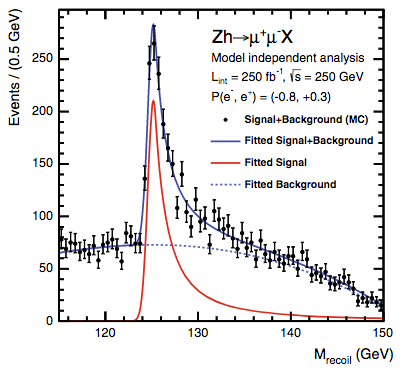
\includegraphics[width=0.5\linewidth]{chap2/fig/HiggsRecoilMuMu.png}
  \caption{The recoil mass distribution for $Zh \rightarrow \mu^+\mu^-X$ at $\sqrt{s}$ = 250 GeV for 250 fb$^{-1}$ integrated luminosity and beam polarisation of (+80\%, -30\%). Simulated with $m_h$ = 125 GeV. Taken from \cite{Thomson2016}} \label{fig:HiggsRecoilMuMu}
\end{figure}

Fits to signal and background are used to extract $m_h$. On can observe a tail to higher reconstructed recoil masses which is coming from events in which initial state radiation (ISR) modified the four momentum of the collision. However this can be accounted for during the reconstruction without shifting systematically the extracted Higgs mass. Combining the two lepton channels, a statistical precision of 32 MeV on the Higgs mass can be achieved, resulting into an uncertainty of 2.5\% on the production cross-section.

\subsubsection{Higgs BR and couplings}

Deviations from the SM Higgs couplings are in the order of less than 1\% in many new physics models beyond the SM. This requires a very high precise measurement of the Higgs coupling strength to the SM particles. At the ILC, the full Higgsstrahlung inclusive production cross-section is proportional to the square of the coupling between the Z and Higgs, $g_{hZZ}$
\begin{equation}
  \sigma(e+e- \rightarrow Zh) \propto g^2_{hZZ}
\end{equation}
The branching ratio of a decay channel is expressed as
\begin{equation}
  BR(h \rightarrow XX) = \frac{\Gamma(h \rightarrow XX)}{\Gamma_{h}}
\end{equation}
where $\Gamma_{h}$ is the full decay width of the Higgs and $\Gamma(h \rightarrow XX)$, the partial decay width with $\Gamma(h \rightarrow XX) \propto g^2_{hXX}$. Typically in a collider, quantity measured is the event rate of a certain final state corresponding to the product of the production cross-section and BR. Thus the final state cross-section at the ILC for the Higgsstrahlung and VBF production is expressed as
\begin{equation}
  \begin{aligned}
    &\sigma(e+e- \rightarrow Zh) \times BR(h \rightarrow XX) \propto \frac{g^2_{hZZ} \times g^2_{hXX}}{\Gamma_{h}}\\
    &\sigma(e+e- \rightarrow h\nu_e\nu_e) \times BR(h \rightarrow XX) \propto \frac{g^2_{hWW} \times g^2_{hXX}}{\Gamma_{h}}
  \end{aligned}
\end{equation}
By measuring the inclusive cross-section $\sigma(e+e- \rightarrow Zh)$ with the recoil technique above, a direct measure of $g_{hZZ}$ is done. A precision of 1.3\% can be achieved for this coupling for 250 fb$^{-1}$ integrated luminosity. The ratio of $\sigma(e+e- \rightarrow Zh)$ and $\sigma(e+e- \rightarrow h\nu_e\nu_e)$ for the same final state of the Higgs (e.g. $h \rightarrow bb$) yields the coupling $g_{hWW}$.

Thus it is only needed to measure the branching ratio $BR(h \rightarrow WW^*)$ to calculate $\Gamma_{h}$. The measurement of $\sigma(e+e- \rightarrow Zh) \times BR(h \rightarrow WW^*)$ and/or $\sigma(e+e- \rightarrow h\nu_e\nu_e) \times BR(h \rightarrow WW^*)$ provide the determination of $\Gamma_{h}$.
\begin{figure}[htbp!]
  \centering
  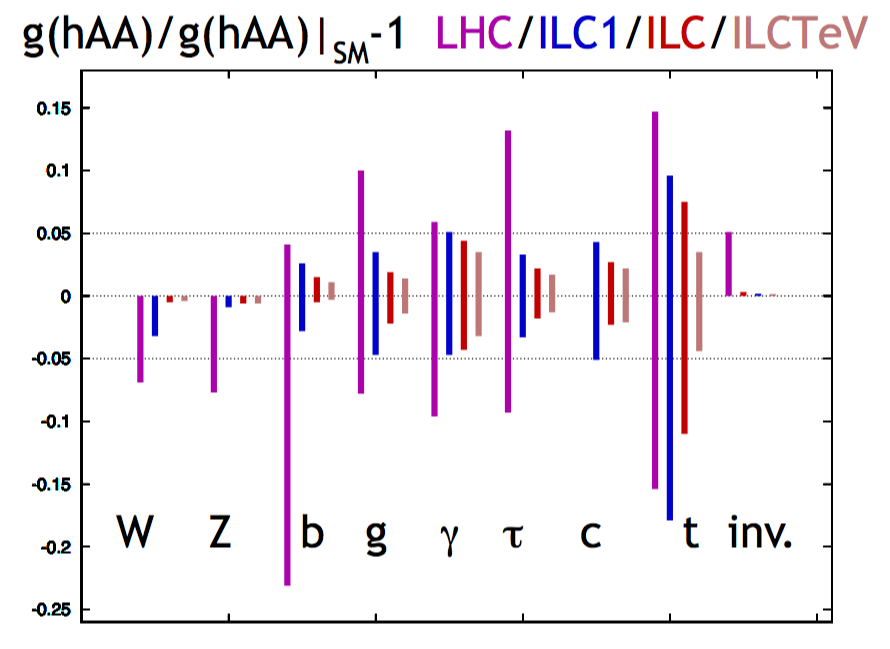
\includegraphics[width=0.6\linewidth]{chap2/fig/HiggsCouplings.png}
  \caption{Relative precision to the Higgs couplings in a model-independent way. 1 $\sigma$ confidence intervals is shown. The four sets are LHC with 300 fb$^{-1}$, 250 fb$^{-1}$ at 250 GeV, 500 fb$^{-1}$ at 500 GeV and the 1 TeV ILC program.}  \label{fig:HiggsCouplings}
\end{figure}

All inclusive cross-section measurements will be included into a global fit to minimize the uncertainty on $\Gamma_{h}$. The figure \ref{fig:HiggsCouplings} shows the relative precision achievable for the ILC compared to the LHC. In most of the measurements, the ILC are one order of magnitude more precise.

\subsubsection{Higgs self-coupling}

The triple Higgs coupling $\lambda$ can be studied at the ILC via the Higgsstrahlung or VBF production starting at around $\sqrt{s}$ = 350 GeV. The cross-section maximizes at around $\sqrt{s}$ = 500 GeV dominated by the Higgsstrahlung production. A study \cite{Duerig:2016dvi} has found that an excess of 3.5$\sigma$ can be detected and the cross-section can be measured to a 30\% precision for 2 ab$^{-1}$ integrated luminosity and a beam polarisation of (-80\%, +30\%). Due to the contribution of irreducible background diagrams without self-coupling, this results in a precision of 49\% on the Higgs self-coupling $\lambda$. At 1 TeV, the measurement of $\lambda$ in the WW channel is opened and leads to a precision of 16\% on $\lambda$ due to smaller contribution of background diagrams.

\subsection{Electroweak Physics}

The ILC gives access to an unprecedented level of precision for the measurement of W and Z masses, widths and couplings. The production processes $e^+e^- \rightarrow W^+W^-$, $e^+e^- \rightarrow ZZ$, $\gamma\gamma \rightarrow W^+W^-$ and triple boson production $e^+e^- \rightarrow VVV$ can be studied. Additionally, vector boson scattering can be studied at high energies to constrain furthermore the Electroweak (EW) sector and search for deviations in the structure of the EW sector of the SM. Many new physics models beyond the SM predict new couplings to the W and Z bosons, thus mixing effects of the new bosons could be detected by the ILC precision measurements.

\subsection{Top mass measurement}

The top quark is the heaviest particle in the Standard Model with a mass of 173 GeV, implying that it is the most strongly coupled particle to the Higgs. The top quark is expected to be one of the most promising window to new physics beyond the SM at the TeV energy scale. The top quark was discovered at the Tevatron by the D0 and CDF experiments \cite{Abe:1995hr, D0:1995jca}, and has only been studied by hadron colliders so far. The ILC would be the first machine to study the top quark using a leptonic initial state.

The top quark has a very short lifetime ($10^{-25}$ s), the top quark decays before hadronisation thus the top quark is a "bare" quark. It decays almost to only $t \rightarrow W^+b$ were the b quark is almost only left handed polarized. At the ILC, the top quark mass can be measured at threshold of $\sqrt{s} \sim 2 m_t$ as the machine can be tuned in energy. Thus the shape of the top cross-section production can be measured allowing precise measurement of the top mass $m_t$, width $\Gamma_t$ and strong coupling $\alpha_s$. Additionally, the initial polarization state can be tuned to enhance the cross-section. Via this method, the top mass can be measured to a statistical precision of around 30 MeV but the final mass is mostly dominated by theoretical uncertainties of around 100-200 MeV. However, to achieve such precision, it is required to have a b-tagging efficiency and purity better than 90\% and jet energy resolution below 4\%. These requirements are met by the ILC detectors.

\subsection{Beyond the Standard Model}

The Standard Model is so far the most accurate model that describes our universe. But it has still deficiencies in some places such as the origin of mass, the strong CP problem, neutrino masses, matter-antimatter asymmetry, dark matter, gravity and more. Various theories are being developed by theorist to try to answer for these questions. One of these theory is Supersymmetry (SUSY). The ILC has the potential to offer high precision measurement studies of any new particles that could be produced, but unfortunately not discoverable due the high QCD background at the LHC. So far, LHC searches provides limits on the new particles and push the SUSY models towards naturalness with a low value of $M_{\mu} \sim M_Z$. This leads to a particle spectrum of several light super-particles charginos and neutralinos, around 150 GeV in mass, which are mass-degenerated (10-20 GeV mass gap). This would be nearly impossible to detect at the LHC. However, the ILC would have access to this new array of particles.

%!TEX root = ../main.tex
\chapter{Calorimetry and the Particle Flow Concept}
\label{chap:CaloPFA}

In high energy physics, calorimeters are fundamental tools used to measure the energy of particles. This is done by measuring signals from interactions of high energy particles with atoms in matter. This chapter will give a general overview of the physics that describes interactions of particles with matter. Additionally, a brief description of the properties of calorimeters and an introduction to the \textit{Particle Flow Concept} which drives the designs of the calorimeters for ILC will be given.

\section{Particle interaction with matter}
\label{sec:PartInter}

In this section, a description of the physics of the interaction of particles with matter will be given. This includes electromagnetic showers induced by electrons and photons, the energy loss by heavy charged particles and the development of hadronic showers. Moreover, the consequences of these interactions on calorimetric measurements will be discussed.

\subsection{Electromagnetic showers}
\label{subsec:EMShowers}

\subsubsection{Energy loss by charged particles}

High energy electrons lose their energy via different processes depending on their kinetic energy. At low energies, below few tens of MeV, electrons (positrons) lose their energy via ionization primarily with other processes contributing (Bhabha scattering, M\o{}ller scattering...). At energies above 100 MeV, the principal source of energy loss is from \textit{Brems\-strah\-lung} photons due to the Coulomb interaction of the electron in the electric field of the nuclei. The different contributions are shown in figure \ref{fig:ElossEM}. The emitted photons follow an energy spectrum that falls off as $1/E$ \cite{Wigmans:392793}. The transition point where the energy losses due to ionization and Bremsstrahlung are roughly equivalent and is generally referred at critical energy $\epsilon_{c}$. A variation in the definition of this quantity is used by the \acrshort{pdg} where $\epsilon_{c}$ is defined as the energy at which the ionization loss per radiation length $X_0$ \footnote{The definition of $X_0$ is given in \ref{subsubsec:EMcascade}.} is equal to the electron energy. This definition is equivalent to the first one as
\begin{equation}
  \left[\frac{dE}{dx}\right]_{brem} \simeq \frac{E}{X_0}
\end{equation}
The difference between the two definitions is shown in figure \ref{fig:Ec}. $\epsilon_{c}$ is material dependent and for solids can be parametrized as
\begin{equation}
  \epsilon_{c} = \frac{\SI{610}{\mega\eV}}{(Z + 1.24)}
\end{equation}
The critical energy $\epsilon_{c}$ for iron is around \SI{21}{\mega\eV}.

\begin{figure}[htbp!]
  \centering
  \begin{subfigure}[t]{0.49\textwidth}
    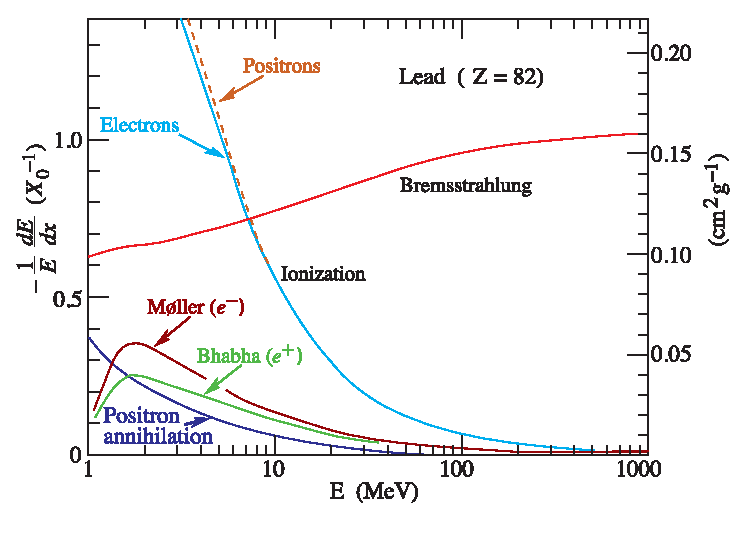
\includegraphics[width=1.\linewidth]{chap2/fig/elossfrac_06.eps}
    \caption{} \label{fig:ElossEM}
  \end{subfigure}
  \hfill
  \begin{subfigure}[t]{0.49\textwidth}
    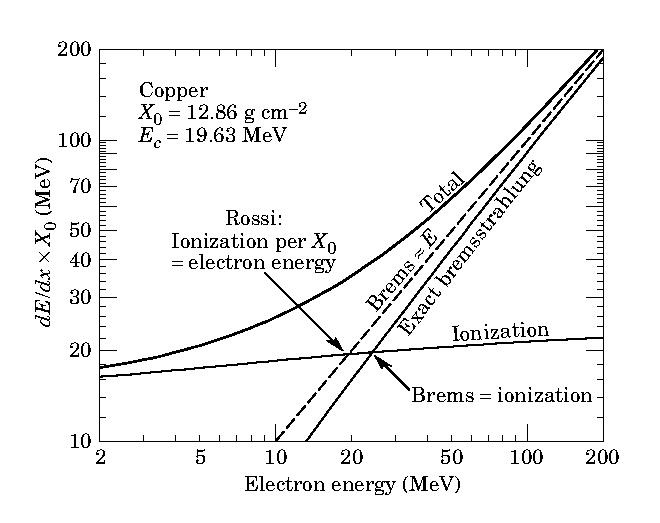
\includegraphics[width=1.\linewidth]{chap2/fig/encrit_cu.eps}
    \caption{} \label{fig:Ec}
  \end{subfigure}
  \caption{\subref{fig:ElossEM}) Fractional energy loss per $X_0$ in lead as function of the electron (positron) energy. \subref{fig:Ec}) Energy losses for electrons in copper for ionization and Bremsstrahlung. The two definitions of $\epsilon_{c}$ are represented \cite{Patrignani:2016xqp}.}
\end{figure}

\subsubsection{Energy loss by photons}

High energy photons lose their energy via \textit{pair production} where the photon creates typically an electron-positron pair caused by the nuclear electric field. However for this process, the photon energy needs to be at least the rest mass of the $e^+e^-$ pair ($E_{\gamma} \geq 2 \times \SI{511}{\kilo\eV}$).

For lower energies between few keV to $\sim$ 5 MeV, it is most likely to interact via \textit{Rayleigh} or \textit{Compton} scattering where the photon is scattered coherently or incoherently by an electron of the atom nuclei. It is one the most important process in the absorption of EM showers as at least half of the energy is deposited in this way.
\begin{figure}[htbp!]
  \centering
  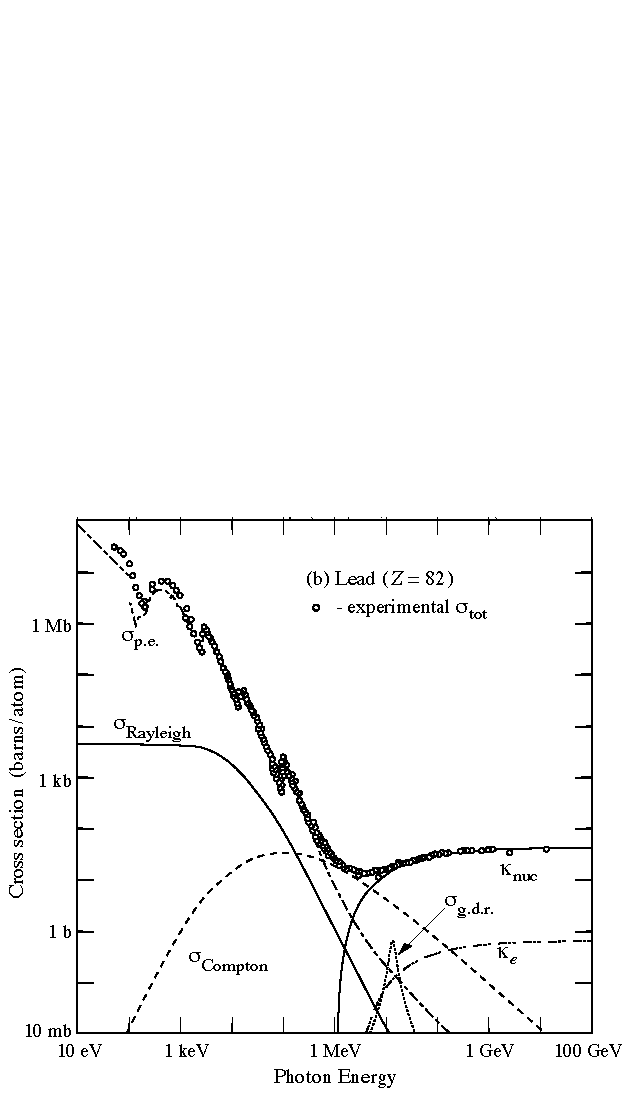
\includegraphics[width=0.5\linewidth]{chap2/fig/sigma_both_06.pdf}
  \caption{Photon total cross-section as function of the photon energy in lead. Adapted from \cite{Patrignani:2016xqp}.} \label{fig:GammaEMloss}
\end{figure}

At the lowest energies, the  \textit{photo-electric effect} is dominant. In this process, the photon is absorbed by the atom and an electron is emitted. The resulted excited atom goes back to ground state by the radiation of Auger electrons or X-rays. This process is very dependent on the $Z$ of the absorber material. The cross-section scales as $Z^n$ with n between 4 and 5 and varies as a function of the photon energy as $E^{-3}$ losing its importance rapidly. The total photon cross-section showing the different processes contributions is shown in figure \ref{fig:GammaEMloss}.

\subsubsection{Electromagnetic cascades}
\label{subsubsec:EMcascade}

A cascade initiated by a multi-GeV electron involves all the processes described above. But Bremsstrahlung plays an important role in EM cascades. An immense number of photons are radiated once it enters matter. Most of these are very soft and thus will get absorbed by Compton scattering and the photo-electric effect. Still, a large number of photons have the necessary energy to go under pair production. These new electrons radiate, in turn, Bremsstrahlung photons creating new branches in the cascade. This results in the multiplication of the number of particles. The number of generated particles in an electron shower is around $\frac{E_0}{\epsilon_{c}}$.

The development of the cascade stops when the average electron energy is around $\epsilon_{c}$. The depth where this occurs is called the \textit{shower maximum} and follows a logarithmic dependence on the initial electron energy such as \cite{Wigmans:392793}
\begin{equation}
  \frac{x}{X_0} = \ln\left(\frac{E_0}{\epsilon_{c}}\right) + C
\end{equation}
with C = -0.5 for electron induced showers and C = 0.5 for photon induced showers. The longitudinal containment of the shower scales similarly with $\ln\left(E_0\right)$. On average, 95\% of the deposited energy of 10 GeV electron is contained within 11 $X_0$ of material, for a 1 TeV electron, around 22 $X_0$ is needed.

Typically EM showers are described by the \textit{radiation length} $X_0$ for the longitudinal development and by the \textit{Moli\`ere radius} $\rho_{M}$ for the lateral development. The radiation length is defined as the distance over which a high energy electron (positron) loses $(1 - e^{-1}) = 63.2\%$ of its initial energy by Bremsstrahlung. A common parametrization of $X_0$ as a function of the atomic number $Z$ and the atomic mass number $A$ is \cite{Wigmans:392793}
\begin{equation}
  X_0 = \frac{716 \times A}{Z(Z+1)\ln\left(287/\sqrt(Z)\right)} [\frac{g}{cm^2}]
\end{equation}
For high energy photons, the radiation length is related to the \textit{mean free path} $\lambda_{\gamma}$, i.e the typical distance in which the photon travels before undergoing pair production as
\begin{equation}
  \lambda_{\gamma} = \frac{9}{7} X_0
\end{equation}

The lateral development of an EM shower is characterized by the Moli\`ere radius $\rho_{M}$. It is given by \cite{Wigmans:392793}
\begin{equation}
  \rho_{M} = \SI{21.2}{\mega\eV} \quad \frac{X_0}{\epsilon_c}
\end{equation}
On average, 90\% of the energy of the shower will be contained into a cylinder of radius $\rho_{M}$.

\subsection{Interaction with charged heavy particles}

As explained above Bremsstrahlung is the main process in which particles lose their energy. But this process is suppressed by the particle mass as $1/m^4$, thus for muons or charged hadrons, ionization is the main process for energy loss. The mean energy loss of a heavy charged particle is given by the Bethe-Bloch formula \cite{Wigmans:392793}
\begin{equation}
  \left<\frac{dE}{dx}\right> = Kz^2\frac{Z}{A}\frac{1}{\beta^2}\left(\frac{1}{2}\ln\frac{2m_ec^2\beta^2\gamma^2T_{max}}{I^2} - \beta^2 - \frac{\delta}{2}\right)
\end{equation}
with $T_{max}$ the maximum single collision energy transfer, $I$ the mean excitation energy of the absorber, $\delta$ a correction term for density effect depending on $\beta\gamma$, K a constant equals to $4\pi{}N_Ar_e^2m_ec^2$, $\beta$ the particle velocity and $\gamma$ the Lorentz factor. The figure \ref{fig:BetheBloch} shows the mean energy loss for muons in copper as function the particle momentum and $\beta\gamma = \frac{p}{mc}$.

\begin{figure}[htbp!]
  \centering
  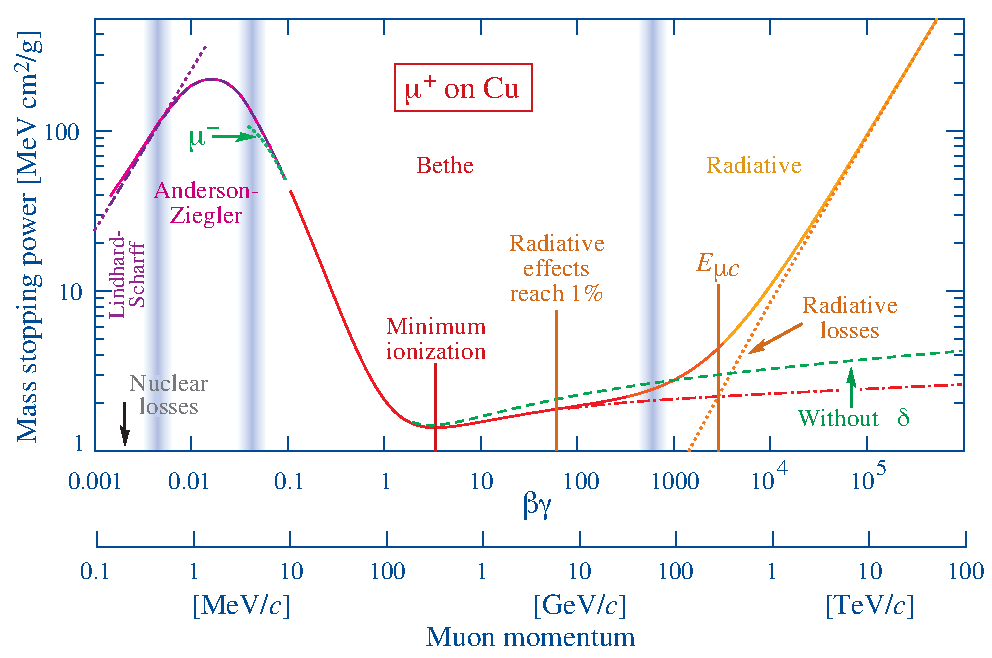
\includegraphics[width=0.7\linewidth]{chap2/fig/rpp_icru49_cu_col.pdf}
  \caption{Mean energy loss of muons in copper as a function of particle momentum. Vertical bands indicate boundaries between model transitions \cite{Patrignani:2016xqp}.} \label{fig:BetheBloch}
\end{figure}

Below 100 GeV, ionization effects dominate in the energy loss and present a broad minimum around 1 GeV ($\beta\gamma \sim 2-4$). Particle in that region are generally referred as \textit{Minimum Ionizing Particles} (\acrshort{mip}). Above 100 GeV, radiative effects become more important than ionization.

However, due to large fluctuations in energy transfer, the mean energy loss may differ from the $\left<\frac{dE}{dx}\right>$ calculation in "relatively" thin materials. The energy loss distribution can be described by a Laudau-Vavilov distribution. The most probable value (MPV) for the energy loss distribution is below the value of $\left<\frac{dE}{dx}\right>$ by around 60\% and has a long tail toward high energy losses due to:
\begin{itemize}
  \item The production of $\delta$-electrons when a significant amount of energy is transferred in a collision
  \item Bremsstrahlung photons that initiate small EM Showers
  \item Nuclear reactions with the nucleus of the material giving rise to high local energy deposits
\end{itemize}
For thick materials, the distribution becomes more Gaussian-like.

\subsection{Hadronic showers}
\label{subsec:HadShowers}

Due to the strong interaction, hadronic showers are more complicated than electromagnetic showers. The physical processes that occur in a hadronic shower are various and much larger in number involving both the incoming particle and the nucleus of the absorber material.

When a charged or neutral hadron penetrates matter, some of the processes described above may be involved. If the hadron is charged, it will ionize the atom of the medium much like a muon. However, at a certain depth, the hadron will, in general, interact strongly with an atom of the medium. This depth can be characterized by a longitudinal scale like EM shower with the radiation length $X_0$. This scale is called the nuclear interaction length $\lambda_n$ generally much larger than $X_0$ (e.g in iron, $\lambda_n/X_0 \sim 9.5$). Similar to EM showers, the longitudinal depth of the shower increases logarithmically with the energy of the incoming hadron.

For neutral hadrons, no ionization is possible and they may lose energy only via nuclear reactions.
\begin{figure}[htbp!]
  \centering
  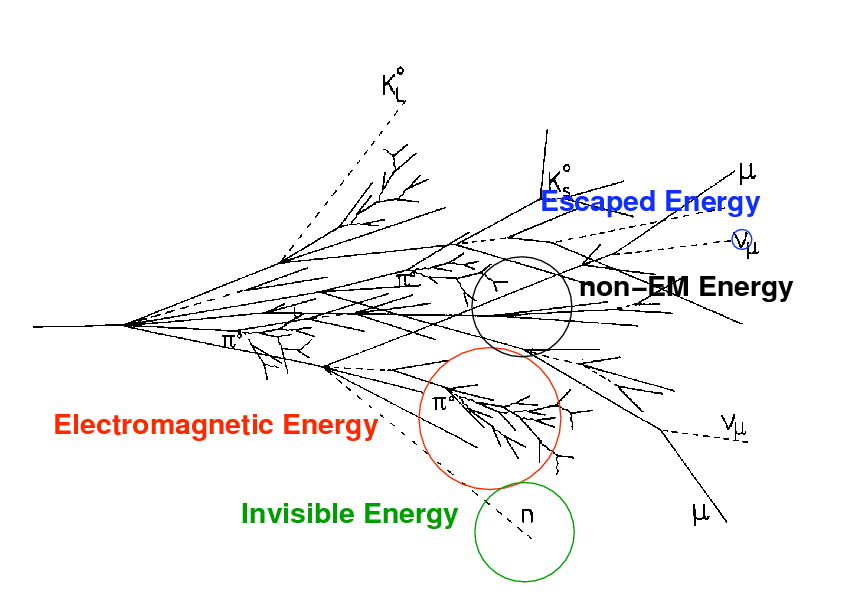
\includegraphics[width=0.7\linewidth]{chap2/fig/images_had-shower.png}
  \caption{Schematic of a hadronic shower. The different "types" of energy are represented in colors. Electromagnetic energy: decay of $\pi^0$s and $\eta$s to $\gamma$s. Non-EM energy: ionization by charged hadrons, spallation. Escaped energy: neutrinos from hadron decays. Invisible energy: nuclear binding energy, neutron scattering and capture \cite{Grahn:2009ki}.} \label{fig:HadShower}
\end{figure}

In general, hadronic shower can be characterized by two components, an electromagnetic component and a hadronic component. A representation of the development of a hadronic shower is shown in figure \ref{fig:HadShower}.

\subsubsection{Electromagnetic component}

When a hadron interacts strongly with the medium, it produces a number of secondary particles, in particular, $\pi^0$s and $\eta$s, which have a very short life ($\sim 10^{-7}$s) and decay electromagnetically to photons such as
\begin{equation*}
  \begin{aligned}
    &\pi^0 \rightarrow 2\gamma \quad (99\%)\\
    &\eta \rightarrow 2\gamma \quad (39\%)\\
    &\eta \rightarrow 3\pi^0 \quad (33\%)\\
    &\eta \rightarrow \pi^0 + 2\gamma \quad (0.03\%)
  \end{aligned}
\end{equation*}
Per hadron collision, on average, 1/3 of the available energy will be carried by the EM component. If the initial energy of the projectile is sufficient after $n$ generations of reactions, the total electromagnetic fraction $f_{EM}$ can be parametrized as \cite{Wigmans:392793}
\begin{equation}
  f_{EM} = 1 - (1 - \frac{1}{3})^n
\end{equation}
However, this is a very simplified model and should be seen only as an upper limit due to other effects (baryon number conservation, ionization and nuclear excitations...) which lower the average electromagnetic fraction. A more accurate representation can be \cite{Wigmans:392793}
\begin{equation}
  f_{EM} = 1 - <m>^{n(k-1)}
\end{equation}
with $<m>$, the average particle multiplicity and the exponent $k$ relating the energy dependence of the EM fraction, function of the pion production threshold $E_0$ and the average fraction of pion production $f_{\pi^0}$. Typically, $f_{EM}$ increase as function of the initial particle energy. For example, a 10 GeV pion in copper\footnote{With the following parameters: $E_0$ = 0.7 GeV, $k$ = 0.82, $f_{\pi^0}$ = 1/4.} has $<f_{EM}> = 0.38$ and at 1 TeV $<f_{EM}> = 0.73$ \cite{Wigmans:392793}.

\subsubsection{Hadronic component}
\label{subsubsec:HadComp}

When a high energy hadron interacts with a nucleus, several processes are possible due to the strong interaction: \textit{spallation}, \textit{evaporation} and \textit{fission}.

Spallation is the most probable interaction. This process can be described in two stages: a fast intra-nuclear cascade involving the constituents of the nucleus and a slow nuclear evaporation. In the first stage, the incoming hadron interacts strongly with the nucleons of the nucleus producing a cascade of new stable and unstable hadrons. The resulting hadrons can then, in turn, go under interaction with a nucleus or decay.

The second stage consists of the de-excitation of the nucleus by evaporating free nucleons until the excitation energy is less than the binding energy of the nucleus. This binding energy is often called \textit{invisible energy} as it is lost during the measurement process. Nevertheless, this energy can be regained by using materials with high fission cross-section such as $^{238}U$.

During spallation, plenty of neutrons can be released. These neutrons are \textit{invisible} to the calorimeter and undergo scattering through the calorimeter (mean free path $\sim$ cm) until they lost most of their kinetic energy (\textit{thermalization}). Then these neutrons can get captured by a nucleus as the capture cross-section is maximal at rest. This process leads to late energy depositions ($\sim$ min). The excited nucleus emits $\gamma$-rays usually to get rid of the excess energy.

Since the \textit{invisible} energy only occurs in hadron showers, this leads to a difference of the calorimeter response between electrons and hadrons of the same energy. This introduces the term of \textit{compensation} that will be described in \ref{subsec:Compensation}.

\subsubsection{Time development}

EM cascades develop at the speed of light due to the prompt generation of particles with relativistic energies. However, hadronic cascades have different components which have an impact on the time development of the shower. The EM component is prompt as an EM cascade but the hadronic component can be delayed significantly due to nuclear excited states ($\sim$\si{\micro\second}) and the release of thermal neutrons ($\sim$\si{\micro\second}-\si{\second}). Thermal neutrons can travel significantly through the detector before being captured by a nucleus and generate a signal in the calorimeter. These effects have an impact on the time acceptance of the readout electronics and thus on the reconstructed energy and spatial development of the shower.

\section{Calorimeters}

Calorimeters are used to absorb a particle and then measure the deposited energy. As explained in \ref{subsec:EMShowers} and \ref{subsec:HadShowers}, the longitudinal depth of the shower scales logarithmically with the energy of the incoming particle. Thus the energy of a shower can be mostly contained completely with a moderate amount of material, even for very high energy particles.

\subsection{General considerations}

Calorimeters can be separated in two types: \textit{homogenous} and \textit{sampling} calorimeters. In homogenous calorimeters, the complete detector volume is sensitive to particle energy depositions. On the contrary, sampling calorimeters, the calorimeter is divided into a passive medium, the absorber that can be made of usually a high-density material, and active medium that generates the signal to be measured.

Sampling calorimeters offer the freedom to chose both the absorber and active material. The absorber can be chosen to minimize the amount of material while still containing most of the energy of the shower. Active materials can be chosen for special purposes, e.g an organic material with high hydrogen content to recover a part of the \textit{invisible energy} by absorbing more neutrons. Also, this allows for optimization of the design and cost. Nevertheless, it has the disadvantage of worse energy resolution than homogenous calorimeters due to sampling fluctuations as only a fraction of the energy of a shower is measured.

A sampling calorimeter can be characterized by its sampling fraction $f_{samp}$ as
\begin{equation}
  f_{samp} = \frac{E_{MIP}^{active}}{E_{MIP}^{active} + E_{MIP}^{passive}}
\end{equation}

Usually calorimeters are segmented longitudinally and laterally into small cells in order to provide information about the particle position.

An example of homogenous calorimeter is the CMS electromagnetic calorimeter. It uses $PbWO_4$ scintillating crystals of around $2.2 \times 2.2 \times 2.3 cm^3$, these have very short radiation length ($X_0$ = 0.85 cm) and Moli\'ere Radius ($\rho_M$ = 2.19 cm) allowing for a compact design. As this calorimeter is homogenous, the entire kinetic energy of an incoming electron or photon can be measured, reducing sampling fluctuations and achieving a very good single particle energy resolution\footnote{Explained in \ref{subsec:EnergyReso}.} of $\sigma_E/E = 2.8\%/\sqrt(E) + 0.3\% + 0.128/E$ \cite{1742-6596-587-1-012001}.

An example of a sampling calorimeter is the ATLAS barrel hadronic calorimeter (TileCal). It consists of iron plates 14 mm thick as absorber and scintillator tiles 3 mm thick as active material. The total depth of the barrel corresponds to 9.7 nuclear interaction length. It is segmented in $\phi$ and $\eta$ to provide accurate position measurement. The tiles are coupled to a wavelength shifting fiber that guides the light to two different photomultiplier tubes providing redundancy. It is the central detector for the measurements of single hadrons, jets and missing transverse energy. An energy resolution of $\sigma_E/E = 52\%/\sqrt(E) + 3\% + 1.6/E$ was achieved for single pions with the Liquid Argon ECAL in front \cite{Henriques:2015fso}. This is significantly worse compared to the CMS ECAL due to the sampling fluctuations and as well due to the intrinsic fluctuations of hadron showers.

\subsection{Energy resolution}
\label{subsec:EnergyReso}

The figure of merit of every calorimeter is the energy resolution. For EM showers, the energy resolution is limited by fluctuations in the shower development. For hadronic showers, these fluctuations are even larger due to large fluctuations in the EM fraction and the average invisible energy. This can be mitigated by compensation or by measuring the EM fraction for each event.
The energy resolution $\sigma_E/E$ can be parametrized as:
\begin{equation} \label{eq:EnergyReso}
  \frac{\sigma_E}{E} = \frac{a}{\sqrt(E)} \oplus b \oplus \frac{c}{E}
\end{equation}

The first term $\frac{a}{\sqrt(E)}$ is the stochastic term. Assuming that $N$ particles contributed to the signal, the uncertainty follows a Poisson statistic (Gaussian if $N$ > 10) such as $\sigma_N/N = \sqrt{N}/N = 1/\sqrt{N}$. Thus the stochastic term for the energy resolution follow this. Additionally, the sampling fraction $f_{samp}$ adds an additional uncertainty proportional to $\sqrt{1/f_{samp}}$. For hadronic showers, the fluctuations in the invisible energy also scales as $1/\sqrt(E)$ and the fluctuations in the electromagnetic fraction scales as $1/E^j$ with $j \leq 0.5$. For EM calorimeter, the stochastic contribution is in the order of few percent for homogenous up to around $10\%/\sqrt(E)$ for sampling calorimeters. Typically, the contribution for hadronic calorimeters is in the order of $60\%/\sqrt(E)$.

The second term $b$ is the constant term. This term is affected by detector inhomogeneities such as calibration uncertainties. This term dominates at high energies and is typically in the order of few percent.

The third term $\frac{c}{E}$ is the noise term. It is energy independent and arises from different effects like the readout electronics. This term dominates at low energies.

\subsection{Compensation}
\label{subsec:Compensation}

As explained in \ref{subsubsec:HadComp}, the invisible energy in a hadron shower initiated by a $\pi$ lowers the calorimeter response compare to an EM shower from an electron of the same energy. The response ratio $e/\pi$ is over 1. This is called \textit{non-compensation}. Moreover, this ratio decreases with energy as the electromagnetic fraction increases with energy. The pion response of a calorimeter can be parametrized as
\begin{equation}
  \pi = <f_{EM}> \times e + (1 - <f_{EM}>) \times h
\end{equation}
with $e$ and $h$ representing the calorimeter response to EM and non-EM fractions. Thus $e/\pi$ can be written as
\begin{equation}
  e/\pi = \frac{e/h}{1 - <f_{EM}>\left(1 - e/h\right)}
\end{equation}

Homogenous calorimeters have generally a significantly higher ratio $e/h \sim 2$. Sampling calorimeter can be designed to reach $e/h \sim 1$. To reach compensation, either the EM response can be lowered or the hadronic response can be boosted. A famous example is the ZEUS calorimeter that used uranium (Z = 92) absorbers and plastic scintillator as active material. The thicknesses of the absorber and active material were carefully optimized to reach compensation. In this way, an energy resolution for pions of $\sigma_E/E = 35\%/\sqrt(E) + 2\%$ was achieved with $e/h \sim 1$ \cite{BERNSTEIN199323}.

Other methods can be used to achieve compensation:
\begin{itemize}
  \item \textit{Dual readout} using Cherenkov radiation to estimate the electromagnetic fraction of each event \cite{Akchurin:2013yaa}.
  \item \textit{Spacial resolution} in order to identify EM sub-showers within a hadronic shower and re-weight the whole shower or individual hits of the shower. This has been demonstrated for the H1 experiment \cite{Schacht:1990zw}. A similar method, called \textit{Offline software} compensation can be done by assigning weights to calorimeter hits as a function of its energy density \cite{SoftCompNew2012}.
\end{itemize}

\section{The Particle Flow approach}
\label{sec:PFA}

Calorimeters are used to measure the energy of single particles and jets. Classically, the energy is reconstructed by summing up all the depositions in the EM and hadronic calorimeters. In this way, typically the stochastic term from equation \ref{eq:EnergyReso} for jets is in the order of $60-100\%\sqrt{E}$. As discussed in chapter \ref{chap:FutureColliders}, this jet energy resolution is far beyond the requirements of the ILC physics program. A new approach has been developed to solve this issue and its concept is presented in this section.

\subsection{The Particle Flow concept}

Particle Flow is a new approach to calorimetry in order to achieve a jet energy resolution much better than traditional calorimetry approaches (order of twice better). It has a potential to revolutionize particle detector design for future lepton collider experiment. \textit{Particle Flow Algorithms} (\acrshort{pfa}) have the ability to reconstruct the energy of all the individual contributions inside a jet. This was made possible by the significant improvements in tracking detectors and calorimeters over the last decade.

\begin{figure}[htbp!]
  \centering
  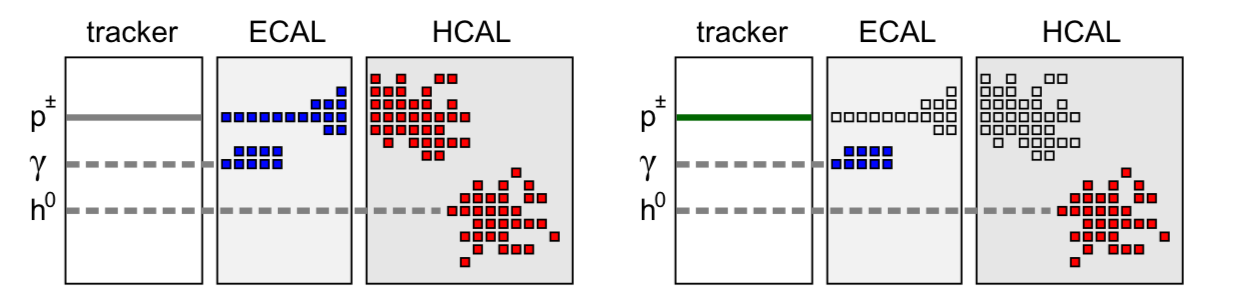
\includegraphics[width=1\linewidth]{chap2/fig/PFAConcept.png}
  \caption{Schematic of the Particle Flow Concept. On the left: Traditional calorimetry, The ECAL and HCAL measure the energy deposited by all particles in a jet (charged particles, photons and neutral particles). The tracker information is not used. On the right: Particle flow approach, The tracker measures all charged particles and the calorimeter information is removed, the ECAL measures the photons and the HCAL measures only neutral particles \cite{Feege:2011dsa}.} \label{fig:PFAConcept}
\end{figure}

On average in a jet, 60\% of the energy is carried by charged hadrons, 30\% by photons and 10\% by neutral hadrons \cite{Ebrahimi:394104}. As hadronic calorimeters have a poor energy resolution ($\sim 60\%/\sqrt{E}$), by traditional approach, 70\% of the energy would be poorly measured. Therefore, the poor resolution of the HCAL is dominant in the jet energy resolution.

Some implementations of PFAs were made in the past like H1 at HERA \cite{Abt:1994ye} and up to now in CMS at the LHC \cite{Sirunyan:2017ulk}. However, these detectors were not designed and optimized for particle flow reconstruction. The ILC detectors are designed in such a way that they offer the best instrumentation for the application of the particle flow concept.

The Particle Flow reconstruction requires an unprecedented longitudinal and lateral segmentations for the calorimeters as well an excellent tracking system. This approach uses the best sub-detector measurement for each particle in a jet. All charged particle are measured by the tracker due to the excellent tracker resolution, photons are measured in the ECAL and neutral hadrons are measured in the HCAL. In this case, only around 10\% of the energy is measured poorly by the HCAL and thus its impact on the jet energy resolution is lessened. A schematic of the Particle Flow concept is shown in figure \ref{fig:PFAConcept}.

The Particle flow approach at the ILC has the potential to improve the jet energy resolution to around 3-4\% in the range of 45 to 250 GeV ($\sim 30\%/\sqrt{E}$). The jet energy resolution can be parametrized as
\begin{equation}
  \sigma_{jet} = f_{charged} \cdot \sigma_{Tracker} \oplus f_{\gamma} \cdot \sigma_{ECAL} \oplus f_{neutral} \cdot \sigma_{HCAL} \oplus \sigma_{conf} \oplus \sigma_{leak}
\end{equation}
$\sigma_{Tracker}, \sigma_{ECAL}, \sigma_{HCAL}$ are the energy resolutions of the tracker, ECAL and HCAL respectively, contributing to the jet energy resolution with weighted fractions of the particle type in the event.

$\sigma_{conf}$ represents the confusion term due to the possibility of wrong assignments of tracks and calorimeter energy depositions. There are three main sources of confusion:

\begin{itemize}
  \item A part (or all) of the shower from a charged hadron is reconstructed as a neutral cluster. This lead to the double-counting of energy.
  \item A part (or all) of a neutral shower is associated to a charged shower. This lead to the lost of the energy of the neutral particle, therefore, energy is missing.
  \item The failure to resolve photons close to a charged hadron track leading to the loss of the photon energy.
\end{itemize}

The confusion is a limiting factor in Particle Flow calorimetry and starts to dominates for high jet energies.

Other contributions such as $\sigma_{leak}$ that degrade the jet energy resolution due to leakage in the calorimeter and uninstrumented areas.

\subsection{Implementation in PandoraPFA}

PandoraPFA \cite{Thomson:2009rp, Marshall2013} is an implementation of the Particle Flow Concept for the ILC. It reconstructs individual particles using the information provided by the highly granular calorimeters and the tracker. The algorithm operates in several stages:

\begin{itemize}
  \item Tracks are categorized based on topology. Kinks, V0s from neutral particle decays, e.g $K_s \rightarrow \pi^+\pi^-$, are identified and treated separately by the algorithm.
  \item Calorimeter hits are clustered using a simple cone-based algorithm starting at the front face of the ECAL going to the back of the HCAL. Tracks seeds from the projection of tracks to the front face of the ECAL can be used for the cluster starting point. The clustering algorithm is configured in a way that it tends to split more the energy deposits than accidentally merging particles in this early stage. The clustering follows certain topological rules and exploit the spatial resolution of the calorimeters to minimize clustering mistakes.
  \item The calorimeter clusters are associated to tracks. The algorithm compares the cluster energy and track momentum and other properties such as the track direction at the front face of the ECAL and cluster orientation to make the correct associations.
  \item If the energy of a cluster and the associated momentum of a track don't agree, a statistical re-clustering is performed using different parameters until a better track-cluster compatibility is found.
  \item The algorithm identify photons based on shower profile information in order to recover photons that are merged with a charged hadron shower.
  \item Fragments of hadron showers are identified and the algorithm looks for neutral fragments that are mis-identified coming from nearby charged clusters. These fragments are merged into the parent charged cluster and the track-cluster compatibility is evaluated again.
  \item A Particle Flow Object (PFO) is constructed. Track properties are used for charged particles, the calorimeter information is used for neutral particles.
\end{itemize}

The details of theses stages and possible other stages are described in more details in \cite{Thomson:2009rp}.

The jet energy resolution obtained in ILD with Pandora PFA is shown in figure \ref{fig:ILDPFA}. The figure shows that the jet resolution obtained is much better than in traditional calorimetry. It also shows that the goal of 3-4\% relative jet energy resolution is achieved over a large jet energy range.

\begin{figure}[htbp!]
  \centering
  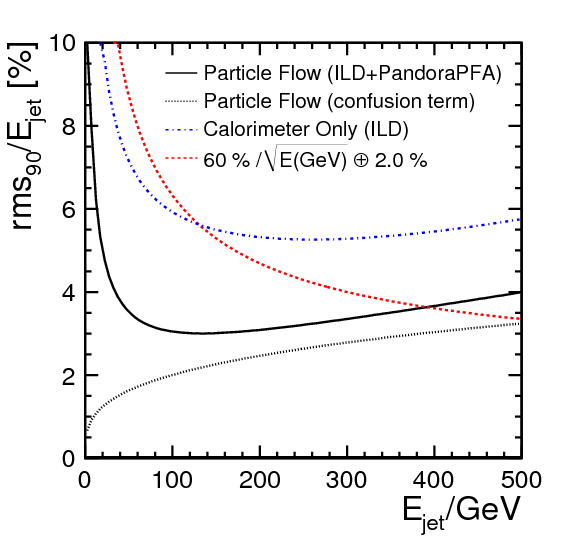
\includegraphics[width=0.6\linewidth]{chap2/fig/pfa_figure_10.png}
  \caption{Empirical jet energy resolution as function of the jet energy for PandoraPFA and the ILD detector. The estimated contribution of confusion is represented by the back dotted line. The dotted-dashed blue curve shows the jet energy resolution only from the calorimetric depositions. Moreover, a parametrization of a typical jet energy resolution ($\frac{60\%}{\sqrt{E}} \oplus 2\%$) is shown in red using the traditional calorimetry approach \cite{Thomson:2009rp}.} \label{fig:ILDPFA}
\end{figure}

\begin{center}
  \rule{0.5\textwidth}{.4pt}
\end{center}

As shown in this chapter, jet energy measurements with an excellent resolution can be achieved with the particle flow approach. This approach requires an excellent tracker and highly granular calorimeters. The development of such calorimeters is discussed in the following chapter.


%% CALICE detectors %%%
%!TEX root = ../main.tex
\chapter{CALICE Calorimeter concepts}
\label{chap:CALICE_Det}

The CALICE Collaboration is developing and testing electromagnetic and hadronic calorimeters. These detector concepts are optimized toward a linear collider environment such as the International Linear Collider (ILC) \cite{ILC_TDR_Vol1} or Compact Linear Collider (CLIC) \cite{CLIC_CDR} but collaboration with the Large Hadron Collider community for the High-Lumi upgrade (HL-LHC) is ongoing \cite{1748-0221-12-01-C01042}. The CALICE calorimeters are high granularity calorimeters optimized for the particle flow algorithm (Pandora PFA) providing a very detailed image of physics events.\\
Several prototypes for physics were build in the past and tested in testbeam campaigns at DESY, CERN and FNAL \cite{1748-0221-3-08-P08001, 1748-0221-5-05-P05004, 1707.07126v2, 1748-0221-10-10-P10039, 1748-0221-3-05-P05001}. Three physics prototypes of 1 m$^3$ were conceived using different active material and absorbers as well different readout schemes.\\
Nowadays, the CALICE Collaboration is still performing analysis on the data collected by these prototypes \cite{OskarCAN, YasmineCAN}. Also, the collaboration is looking forward in the integration into a full linear collider detector by designing several new technological calorimeter prototypes.\\
In this chapter, the electromagnetic and hadronic calorimeter concepts will be introduced, described.

\section{Silicon Photomultipliers}

Semi-conductors detectors have been used since more than 50 years and are still a major research topic in high energy physics \cite{1748-0221-4-04-P04004, Garutti:2011qv, Garutti:2017ipx}. \textit{Silicon photomultipliers} (SiPMs) are semi-conductors used to measure light amplitudes down to the single photon. SiPMs are composed of an array of \textit{Avalanche Photodiodes} (APDs) pixels operated in Geiger-mode. The pixels are all connected in parallel to a common cathode and anode. Nowadays, thousands of pixels can be integrated into a few $mm^2$ area.

Each pixels are operated in reverse bias ($V_{bias}$), in the order of 30-60 V, larger than the \textit{breakdown voltage} ($V_{bd}$). When a photon is absorbed, an electron-hole pair is created in the depletion region by the photo-electric effect. This electron is accelerated by the electric field and starts to create a self-sustained avalanche or \textit{Geiger discharge} by impact ionization, rendering the diode conductive. A serial \textit{quenching resistor} ($R_q$) reduces the effective voltage of the pixel below $V_{bd}$ thus quenching the avalanche. Each pixel deliver a charge $Q$ such as
\begin{equation}
  Q = C_{px} \times (V_{bias} - V_{bd})
\end{equation}
with $C_{px}$ the capacitance of the pixel, typically around few pF and depends on the geometry and doping profile of the pixel. $V_{bias} - V_{bd}$ is the over-voltage or excess voltage over the breakdown voltage.

Following this equation, $Q$ characterizes the gain of the SiPM and is proportional to the over-voltage. $V_{bd}$ is temperature dependent, effectively increasing with the temperature. Thus SiPM gain show an inverse correlation function of the temperature in the range of -1\%/K. Similarly, the \textit{quantum efficiency or photon detection efficiency} (PDE), the probability to initiate a Geiger discharge, has an inverse correlation with temperature and increases with $V_{bias} - V_{bd}$.

Once an avalanche has stopped, the effective voltage of the pixel can return to $V_{bias}$ with the \textit{recovery time} $R_q \cdot C_{px}$ in the order of hundred of nanoseconds before the pixel can fired again. Carriers trapped in defects in the silicon matrix introduce new levels of energy in the conduction band, a release of these carriers causes \textit{afterpulsing} in a period of 50-100 ns after firing.

The measured total charge is the sum of all the fired pixels. With a good uniformity in pixel capacitance and low-noise electronic amplification, the SiPM gain can be measured in-situ by illuminating the SiPM with short and low amplitude light pulses giving a \textit{single-photon spectra} (SPS) as shown in subsection \ref{subsec:GainCharac}.

Due to the finite number of pixels and the recovery time of the pixels in the order of several nanoseconds, the response of a SiPM is non-linear and can be at a first order parametrized as
\begin{equation}
  N_{fired} \approx N_{total} \times (1 - e^{\frac{- N_{\gamma} \cdot PDE}{N_{total}}})
\end{equation}
with $N_{total}$, the total number of pixels, $N_{\gamma}$, the number of incoming photons and $PDE$, the photon detection efficiency. This parametrization can describe the data very well at low light levels but can significantly differ with a high number of photons \cite{Kotera:2015rha}.

An avalanche can be initiated by a photon but also free carriers in the depleted layer. The rate of the latter \textit{dark noise} increases with $V_{bias} - V_{bd}$ and the temperature. A dark rate of 100 kHz to several MHz per mm$^2$ is produced by typical SiPMs. This dark count rate falls dramatically when increasing the threshold of the readout electronics and typically the increase of the threshold by 1 photo-electron amplitude reduces the dark rate by around one order of magnitude.

Geiger avalanches in a pixel can produce photons that can travel to the nearest pixel and trigger an avalanche. This is referred as \textit{optical cross-talk}. This effect is in the order of 3-10\% for typical SiPMs and can be mitigated by reducing the operating voltage, adding an optical absorber or trenches between pixels.

In the last decade, significant improvements in the manufacture of SiPMs have been achieved and are commercially available. The PDE range has been improved to be sensitive down to near ultraviolet light (300-400 nm) up to infrared light (800-1000 nm). The dark noise rates have been reduced as low as few tens of kHz at room temperature. The introduction of trenches between pixels in the substrate have enabled to reduce the cross-talk probability under 1\% \cite{Liu:2015cpe}. Pixel-to-pixel uniformity in capacitance and breakdown voltages improvements reduce the need for individual bias adjustment. And finally, SiPMs with a very high number of pixels ($\geq$10000) are available, improving the range of linear response and increase the dynamic range but at the detriment of noise rates and PDE.

\section{Electromagnetic Calorimeters}

The CALICE Collaboration is developing two different electromagnetic calorimeters (ECAL) concepts. Physics prototypes whose goal was to prove the performance of such calorimeters for detailed measurements of EM showers were first built. Now engineering prototypes are designed in order to improve the calorimeter design, the integration of the front-end electronics and the readout scheme. In the next subsections, the silicon-based SiECAL and the scintillator-based ScECAL calorimeters using both tungsten as absorber material will be described.

\subsection{SiECAL}

The SiECAL physics prototype consists of 30 active and absorber layers. The sensitive layer is made of high-resistivity silicon wafers 525 \si{\micro\meter} thick. These are divided into 6$\times$6 cm$^2$ sensors, segmented into a matrix of 1$\times$1 cm$^2$ PIN diodes operated in reversed bias. The total active area is 18$\times$18 cm$^2$ which resulted in 9720 channels. The depth of the calorimeter was 24 X$_0$ achieved by 10 layers of 0.4 X$_0$ (1.4 mm), followed by 10 layers of 0.8 X$_0$ (2.8 mm) and 10 more layers of 1.2 X$_0$ (4.2 mm) thick tungsten absorber plates. No front-end electronic was integrated into the layers but placed off-detector using analog lines. The performance of such calorimeter was tested in various beams at DESY and CERN. An energy resolution of $\frac{16.53\%}{\sqrt{E}}$ stochastic term and $1.07\%$ constant term was achieved \cite{ADLOFF2009372}.

\begin{figure}[htbp!]
  \centering
  \begin{subfigure}[t]{0.49\textwidth}
    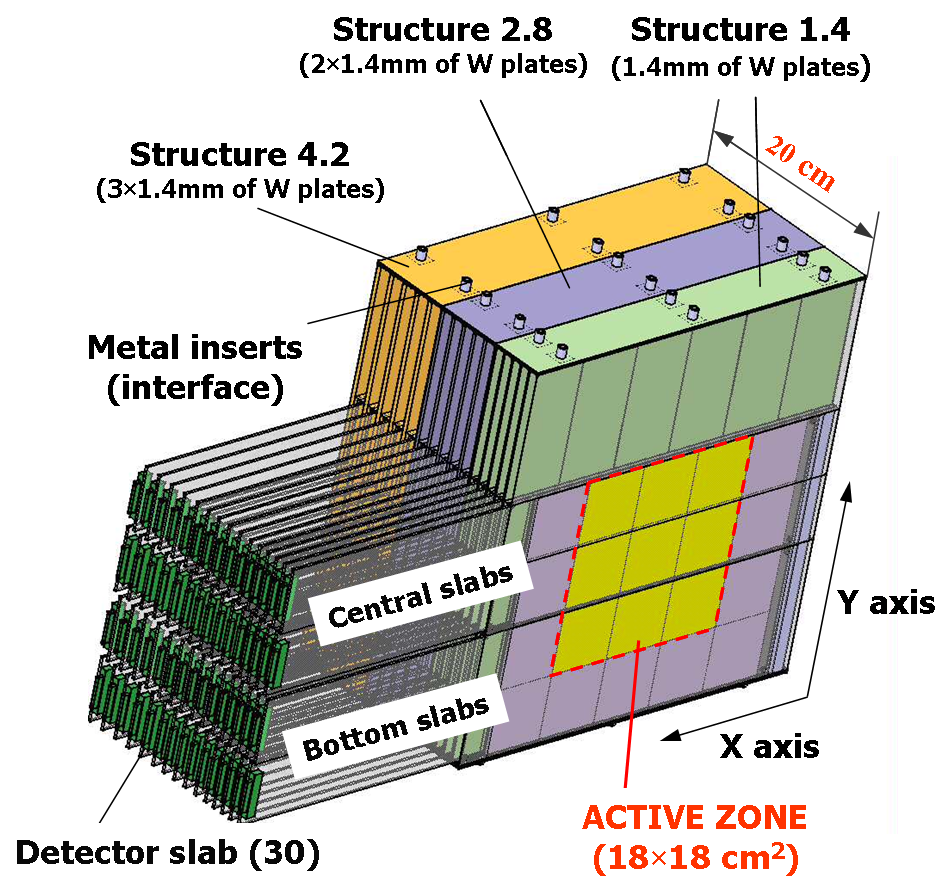
\includegraphics[width=1.\linewidth]{chap3/fig/3DProtoH.png}
    \caption{} \label{fig:SiWECALPhysics}
  \end{subfigure}
  \hfill
  \begin{subfigure}[t]{0.49\textwidth}
    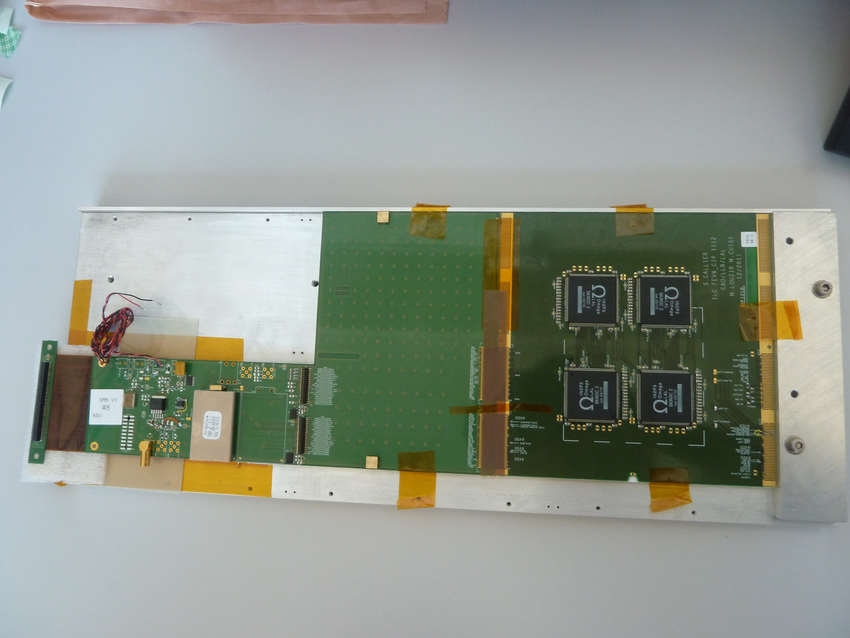
\includegraphics[width=1.\linewidth]{chap3/fig/SiW-ECAL_Techno.png}
    \caption{} \label{fig:SiWECALTechno}
  \end{subfigure}
  \caption{\subref{fig:SiWECALPhysics}) The schematics of the SiW-ECAL physics prototype. \subref{fig:SiWECALTechno}) Picture of a layer of the SiW-ECAL technological prototype.}
\end{figure}

After the validation of the calorimeter concept, a technological SiECAL prototype is being developed focusing on the integration into a full linear collider detector. To do this, modules close to the ILD design are being developed taking into account mass-production and low-power front-end electronics are integrated into the detector volume. The silicon wafers are larger and divided into 9$\times$9 cm$^2$ sensors. The PIN diode matrix is reduced to 5$\times$5 mm$^2$ pads to improve the pattern recognition of the calorimeter. New designs to the sensor are also made to minimize dead area at the sensor edge and cross-talk effects. The front-end is equipped with an ASIC, the SKIROC2 chip \cite{1748-0221-6-12-C12040}. It has 64 channels with adjustable gain charge pre-amplifier, a 12-bit ADC and digital logic. Also, it allows for auto-triggering with an adjustable threshold (below 0.5 MIP) and hit time recording performed on a 12-bit TDC ramp. The SKIROC2 ASIC is designed to match the ILC beam structure (see chapter \ref{chap:FutureColliders}) and thus allows for a power-pulsed mode where electronics are switched off between ILC bunches. This allows a very low power dissipation in the order of 25 \si{\micro\watt} per channel.

\subsection{ScECAL}
\label{subsec:ScECAL}

The ScECAL physics prototype consists of 30 layers of scintillator and tungsten carbide absorber plates 3.5 mm thick. The total calorimeter thickness is 266 mm or 21.5 X$_0$. The layers have a transverse area of 180$\times$180 mm$^2$. Each layer is composed of four rows of 18 scintillator strips of dimensions 45$\times$10$\times$3 mm$^3$ and the strips are placed orthogonally in consecutive layers. The strips have a Wavelength-shifting Fiber (WLS) inside to guide the scintillation light to a Silicon-Photomultiplier (SiPM), a MPPC from Hamamatsu. This accounts for 2160 channels to be read out. This prototype was tested in various beams, an energy resolution of $\frac{12.6\%}{\sqrt{E}}$ stochastic and 1.6\% constant term was demonstrated \cite{1707.07126v2}.

\begin{figure}[htbp!]
  \centering
  \begin{subfigure}[t]{0.49\textwidth}
    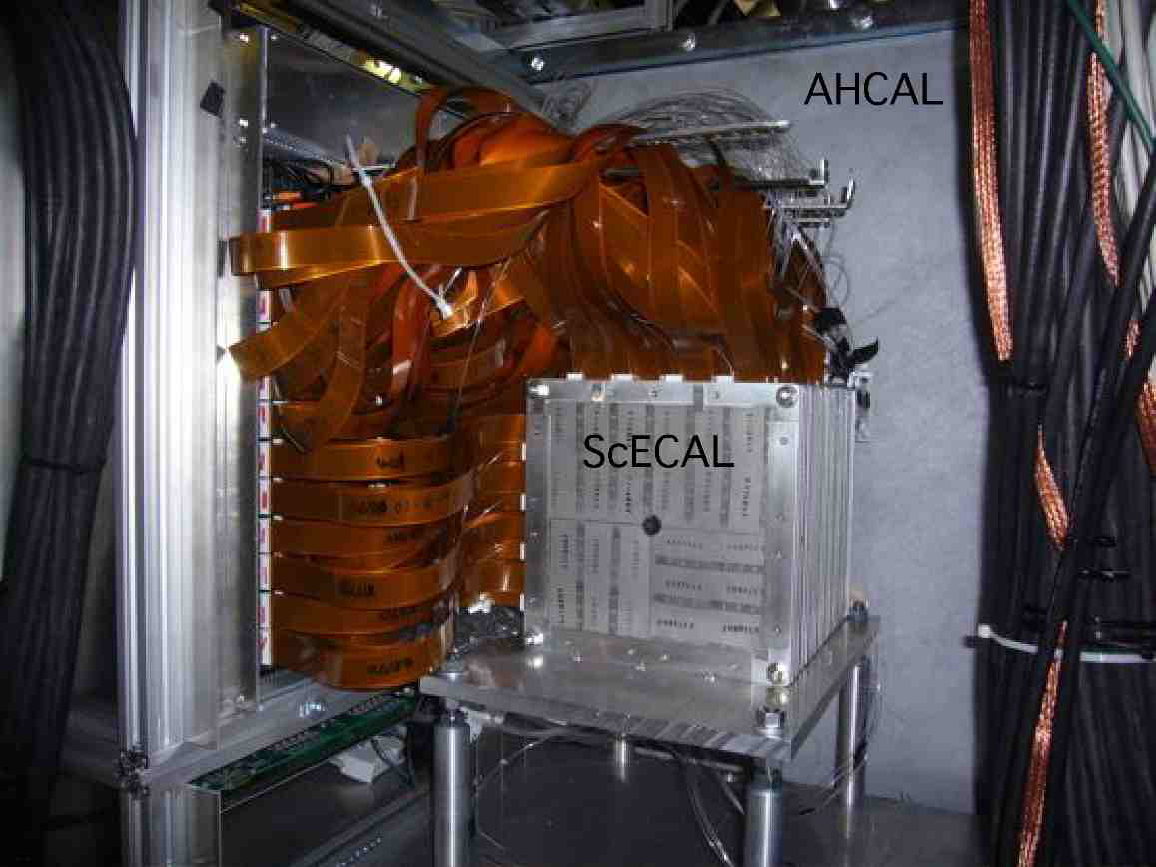
\includegraphics[width=1.\linewidth]{chap3/fig/photo_scecal2.pdf}
    \caption{} \label{fig:ScECALPhysics}
  \end{subfigure}
  \hfill
  \begin{subfigure}[t]{0.49\textwidth}
    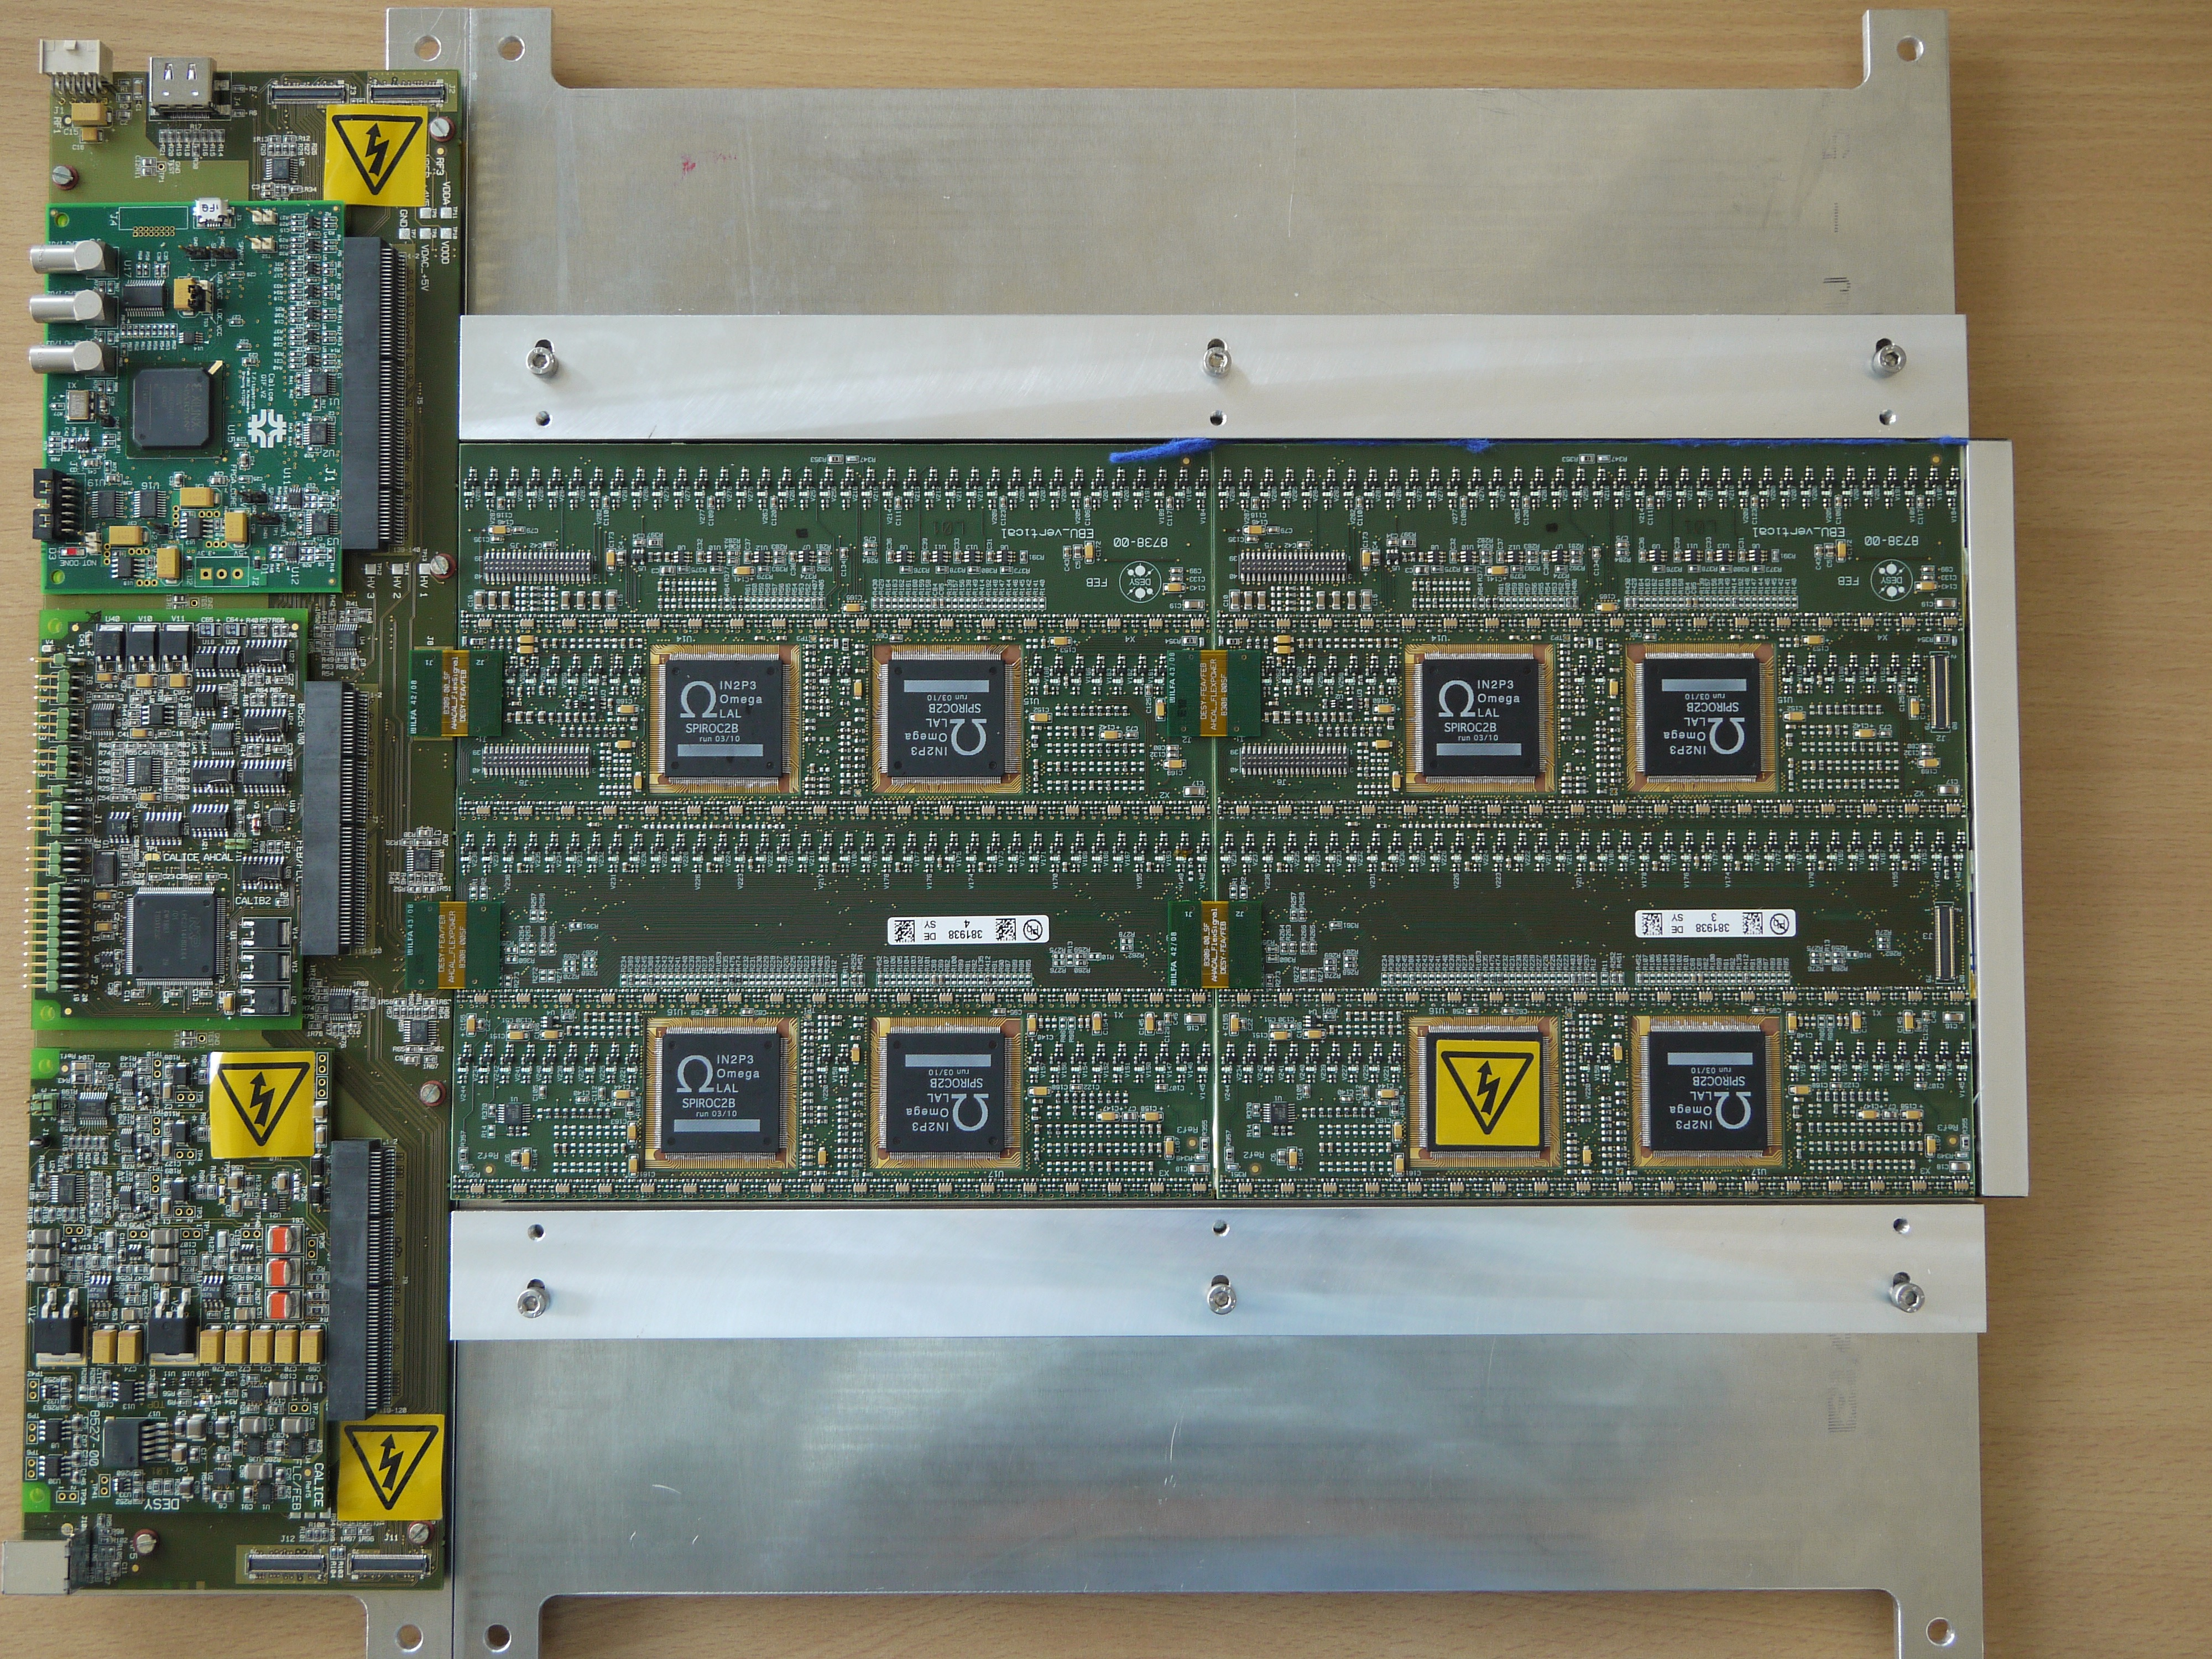
\includegraphics[width=1.\linewidth]{chap3/fig/P1060076.jpeg}
    \caption{} \label{fig:ScECALTechno}
  \end{subfigure}
  \caption{\subref{fig:ScECALPhysics}) Photo of the ScECAL physics prototype with the Fe-AHCAL at FNAL. \subref{fig:ScECALTechno}) Photo of the top side of the technological ScECAL prototype.}
\end{figure}

To look forward, a technological prototype is now developed to accommodate the front-end electronics into the layer to reduce the amount of dead material due to cabling. An ECAL Base Unit (EBU) has 144 scintillator strips of dimensions 45$\times$5$\times$2 mm$^3$. Each layer has a transverse dimension of 180$\times$180 mm$^2$. The strips don't have a WLS fiber due to improvements in SiPM technology for blue light ($\sim$ 450 nm) detection efficiency. Several designs in SiPM and scintillator strip shape are being studied to optimize light collection. In this thesis (see section \ref{sec:TBsetup}), two designs were used in testbeam at CERN, a bottom-side readout and baseline readout design. The former uses 10k pixels surface-mounted MPPC, the latter uses 1.6k pixels MPPC placed on the side of the strips. Each SiPM are read out by an ASIC, the SPIROC2B. Each layer is equipped with four SPIROC ASICs. Each channel has also an integrated LED calibration system in order to monitor the SiPM gain.

\subsubsection{SPIROC2B ASIC}

The SPIROC2B (SiPM Integrated Read-Out Chip) is a dedicated ASIC to readout and digitize the signal of 36 SiPM channels. Each channel can be tuned in bias voltage from -4.5V to 0V with a resolution of around 20-200 mV. Each channel, also, has a configurable charge pre-amplifier gain to cover a high SiPM pixel dynamic range. Each channel is equipped with a capacitor-array, called memory-cells, with a depth of 16 events. A 12-bit Wilkinson ADC is used to digitize the charge stored in the capacitor array for the amplitude and time measurement. The hit time is registered via a 12-bit TDC voltage ramp with a designed resolution of 100 ps if operated in ILC-like conditions (ramp length of 200 \si{\nano\second}), in testbeam, the theoretical time resolution is around 1.9 ns (ramp length of 4 \si{\micro\second}). The chip can be operated in power-pulsing mode where parts of the chips not needed in any given state of operation can be switched off.

\begin{figure}[htbp!]
  \centering
  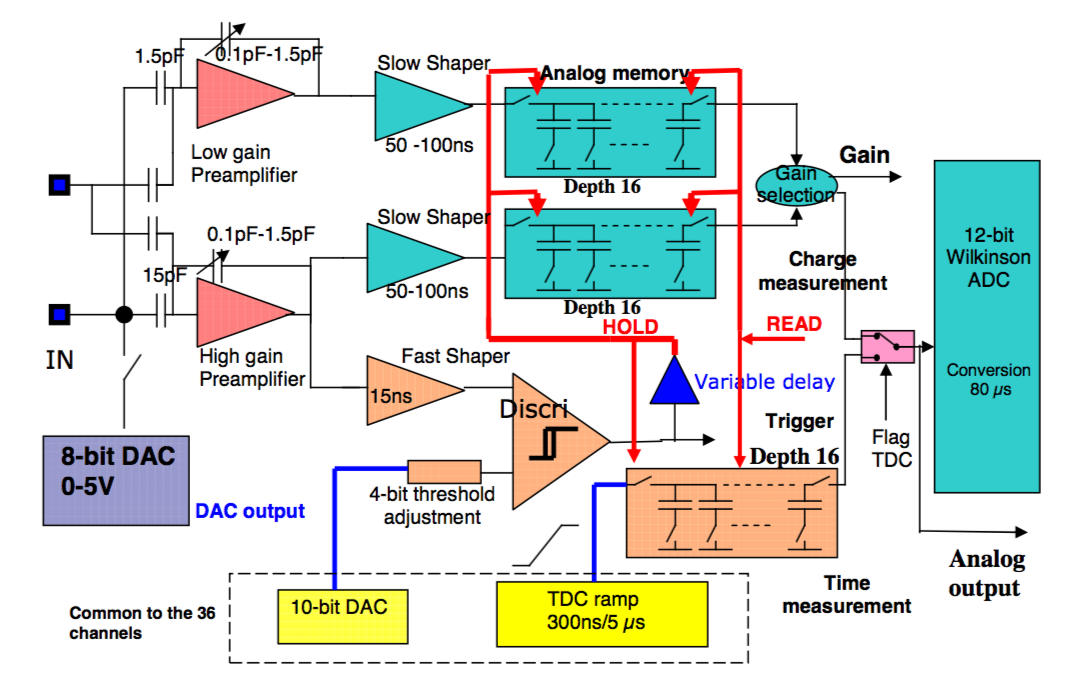
\includegraphics[width=0.7\linewidth]{chap3/fig/SPIROC2B_schematic.png}
  \caption{Schematic of the analog signal path of the SPIROC2 for a single channel \cite{SPIROC2_datasheet}.} \label{fig:SPIROC2B_sche}
\end{figure}

The chip can be operated in either external trigger mode (ET) or auto-trigger mode (AT). In external trigger, the signal of each cell is sampled synchronously to an external signal. In auto-trigger mode, the signal of each cell is compared to a configurable threshold, if the signal is above the threshold, the signal is sampled. Once the 16 memory-cells are filled, no further hits can be stored. Thus, the memory-cells are readout, digitized and the data is transferred out of the chip.

\section{Hadronic Calorimeters}

\subsection{AHCAL}
\label{subsec:SPIROC2B}

The Analog Hadron Calorimeter (AHCAL) is a sampling calorimeter using scintillator tiles has active material. The absorber structure can be either steel or tungsten but I will focus on the former one. The physics prototype consists of 38 active layers inserted in a steel structure of 1 m$^3$ with 39 absorber plates 1$\times$1 m wide and 17.4 mm thick on average. The calorimeter has a total depth of 4.28 $\lambda_{\pi}$ (5.3 $\lambda_{n}$). Active layers are consisted of a steel cassette housing 216, for the 30 first layers, or 141, for the 8 last layers, scintillator tiles connected on a PCB. The tiles are 5 mm thick and have different sizes of 3$\times$3, 6$\times$6, 12$\times$12 cm$^2$. This accounts for a total of 7608 channels. The light produced in the scintillator is guided through a WLS fiber 1 mm thick that is inserted in the tile to a SiPM. The SiPM sensitive area is 1.1$\times$1.1 mm$^2$ containing 1156 pixels which were produced by the MEPhi/PULSAR group in Russia. The performance of this prototype has been demonstrated in several beam types. For electrons, the energy resolution of the AHCAL measured is $\frac{21.7\%}{\sqrt{E}}$ stochastic and <1\% constant term \cite{CAN034}. For pions, the intrinsic energy resolution of the AHCAL has been measured to be $\frac{57.6\%}{\sqrt{E}}$ stochastic and 1.6\% constant term. This can be improved to $\frac{45\%}{\sqrt{E}}$ stochastic term by using a technique called \textit{software compensation} \cite{SoftCompNew2012}.

\begin{figure}[htbp!]
  \centering
  \begin{subfigure}[t]{0.49\textwidth}
    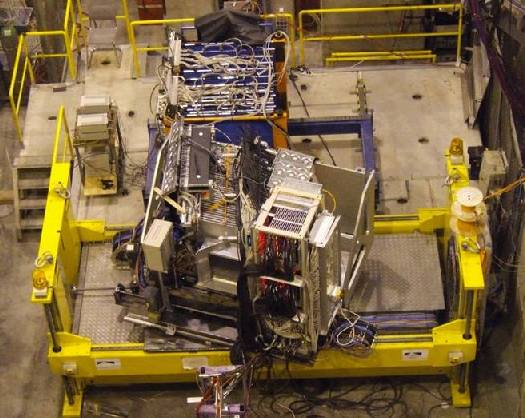
\includegraphics[width=1.\linewidth]{chap3/fig/CERN_setup.png}
    \caption{} \label{fig:AHCALPhysics}
  \end{subfigure}
  \hfill
  \begin{subfigure}[t]{0.49\textwidth}
    \includegraphics[width=1.\linewidth]{chap3/fig/moduleinside.png}
    \caption{} \label{fig:AHCALPhysics2}
  \end{subfigure}
  \caption{\subref{fig:AHCALPhysics}) Photo of the AHCAL physics prototype at CERN. \subref{fig:AHCALPhysics2}) Photo of the active layer of the AHCAL physics prototype showing the layout of the differently sized tiles.}
\end{figure}

The AHCAL engineering prototype (EPT AHCAL) is currently being studied. The goals of this prototype are to demonstrate the scalability of the AHCAL concept to a full linear collider detector. The HCAL Base Unit (HBU), see figure \ref{fig:AHCALHBU}, is 36 cm wide PCB holding 4 SPIROC2B ASICs for a total of 144 SiPM channels coupled to a scintillator tile of 30$\times$30$\times$3 mm size to be read out. Up to 6 HBUs can be connected together to form what is called a \textit{slab}. A full AHCAL layer can be up to 3 slabs connected in parallel to a common set of readout (DIF), calibration (CALIB) and power modules (PWR). An integrated LED Calibration system can deliver LED light pulses with amplitudes to few photons up to saturation of the SiPM in order to calibrated and monitor each HBU channel. Several designs of HBU and tiles have been produced to accommodate for soldering pin or surface-mounted (SMD) type SiPMs. A cross-section of a AHCAL layer is shown in figure \ref{fig:SectionAHCAL}.

\begin{figure}[htbp!]
  \centering
  %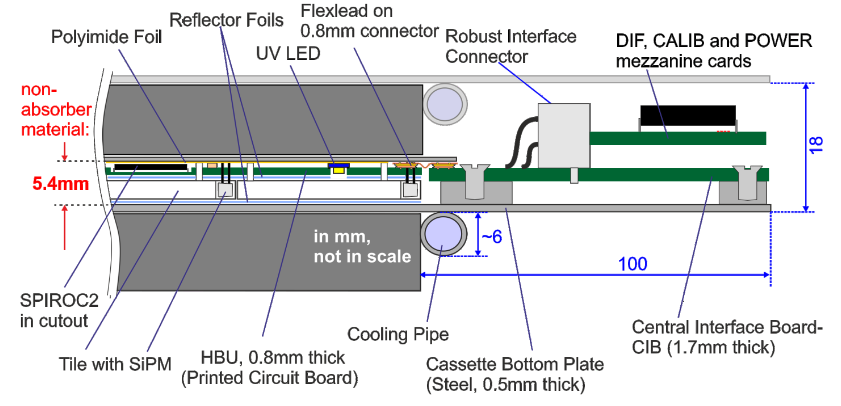
\includegraphics[width=0.8\linewidth]{chap3/fig/AHCAL_section.png}
  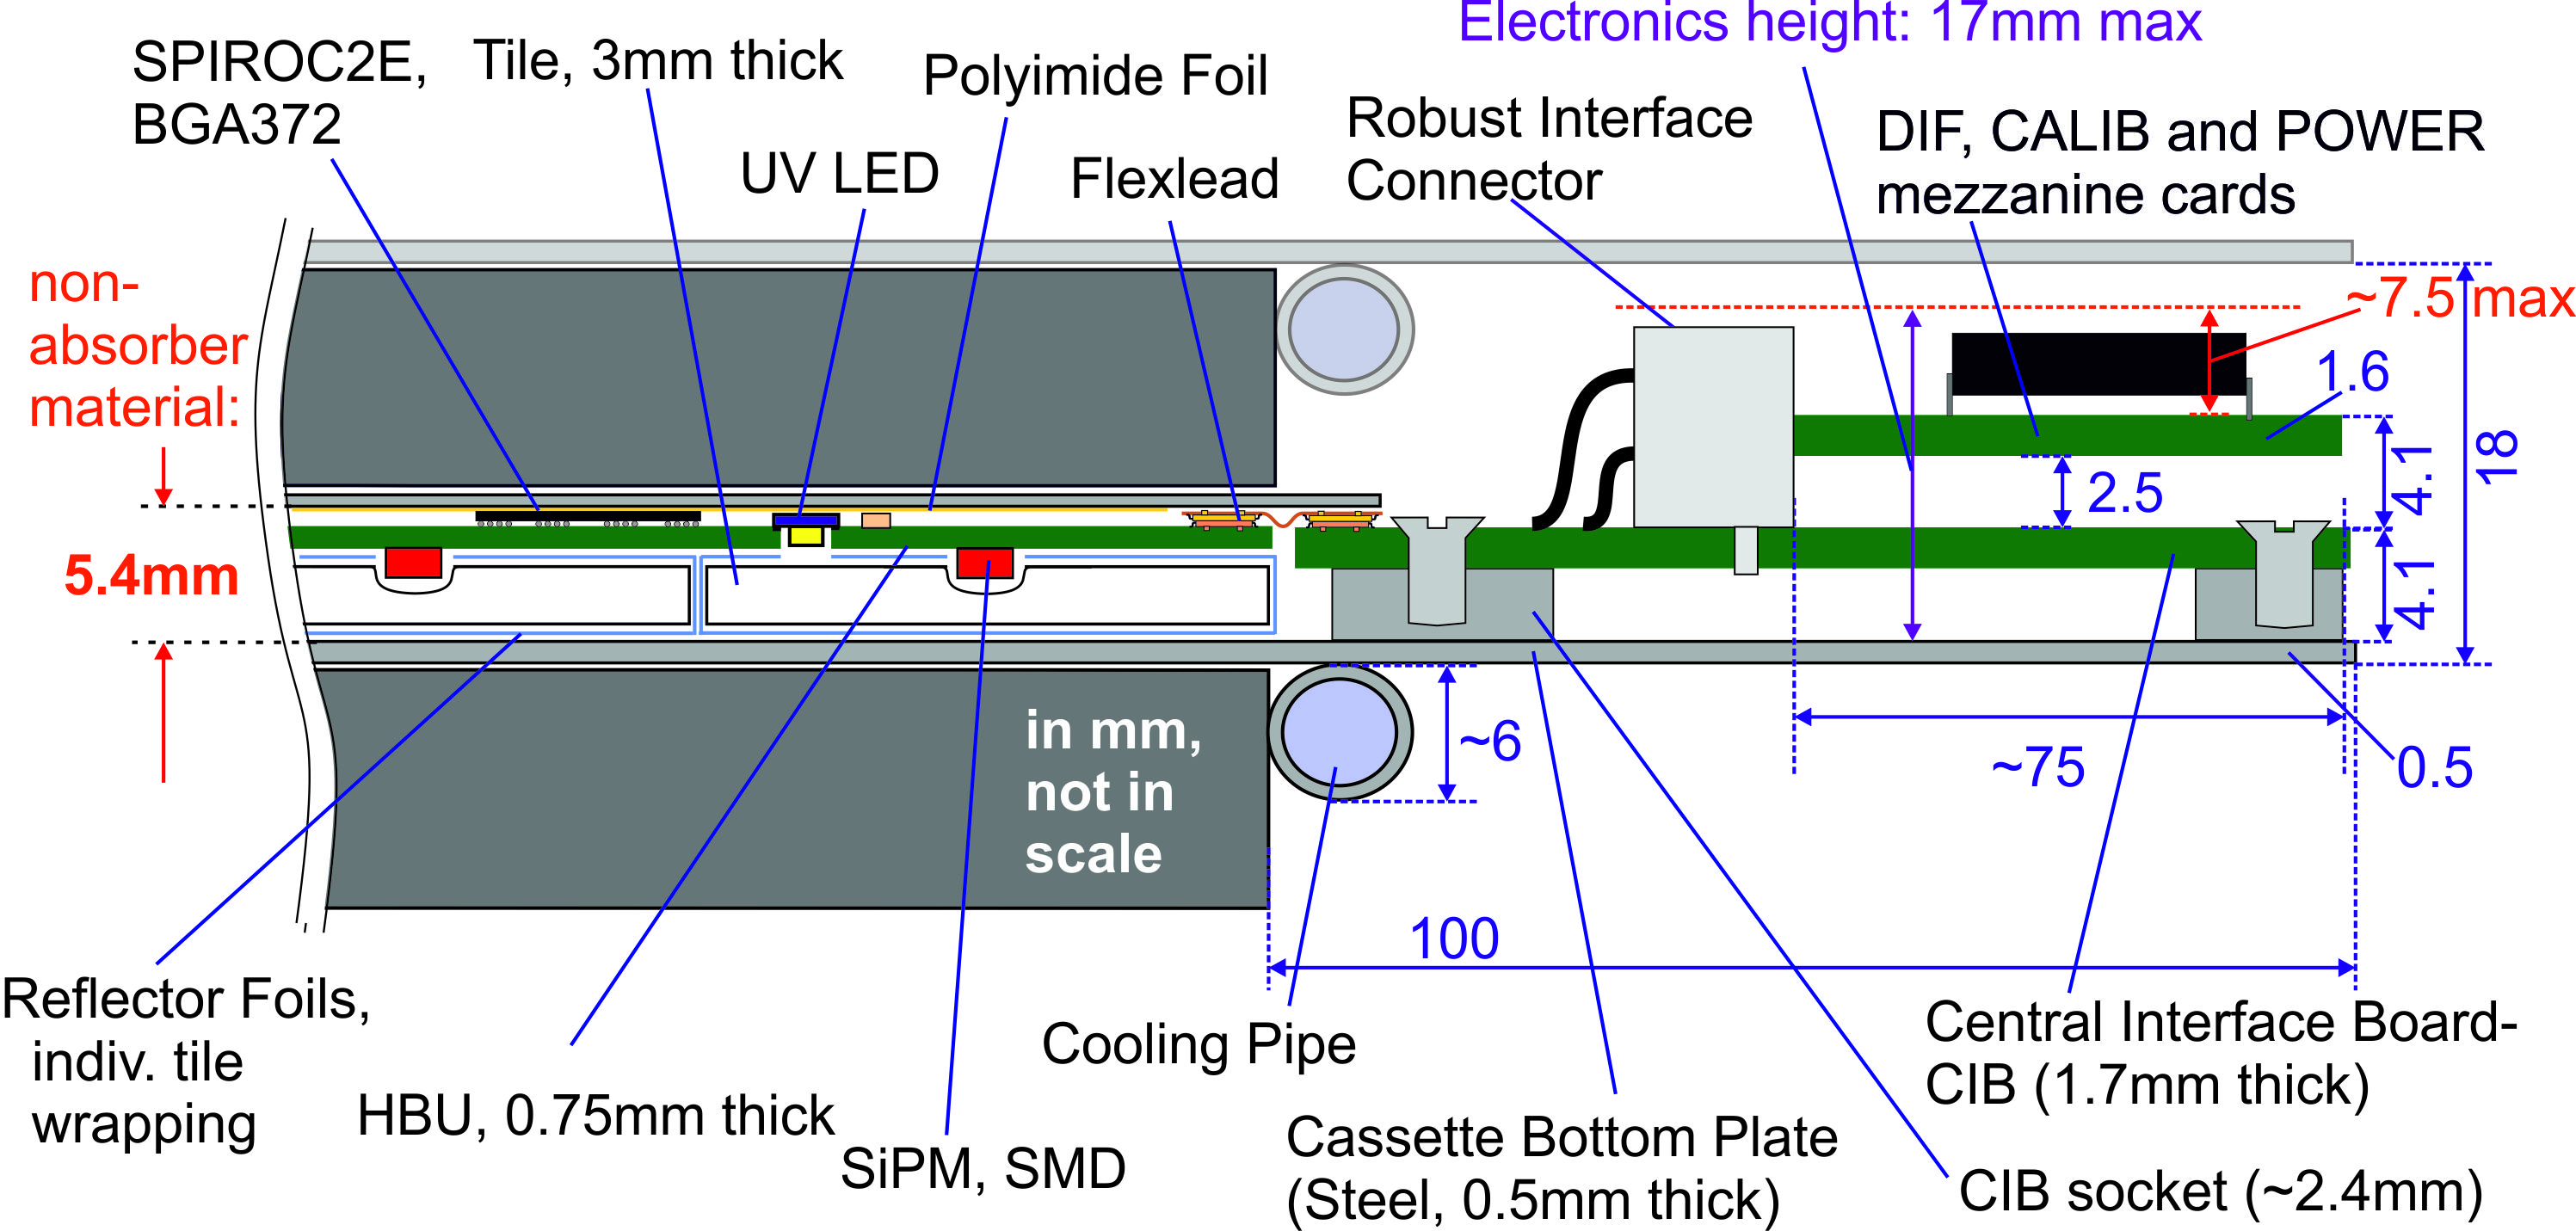
\includegraphics[width=0.8\linewidth]{chap3/fig/HCAL_cross_endface_vers0p4.jpg}
  \caption{Cross-section of a layer in the Fe-AHCAL engineering prototype with the SPIROC2E.} \label{fig:SectionAHCAL}
\end{figure}

\subsubsection{Current status of the EPT AHCAL}

A first step was achieved with the operation of 15 AHCAL layers in testbeam at CERN in July and August 2015. Various HBU designs with many types of SiPMs from different manufacturers have been used and served as a benchmark for the ongoing development of scintillator tiles concepts. These results have been used to focus on a particular tile design for the next generation prototype.
\begin{figure}[htbp!]
  \centering
  \begin{subfigure}[t]{0.37\textwidth}
    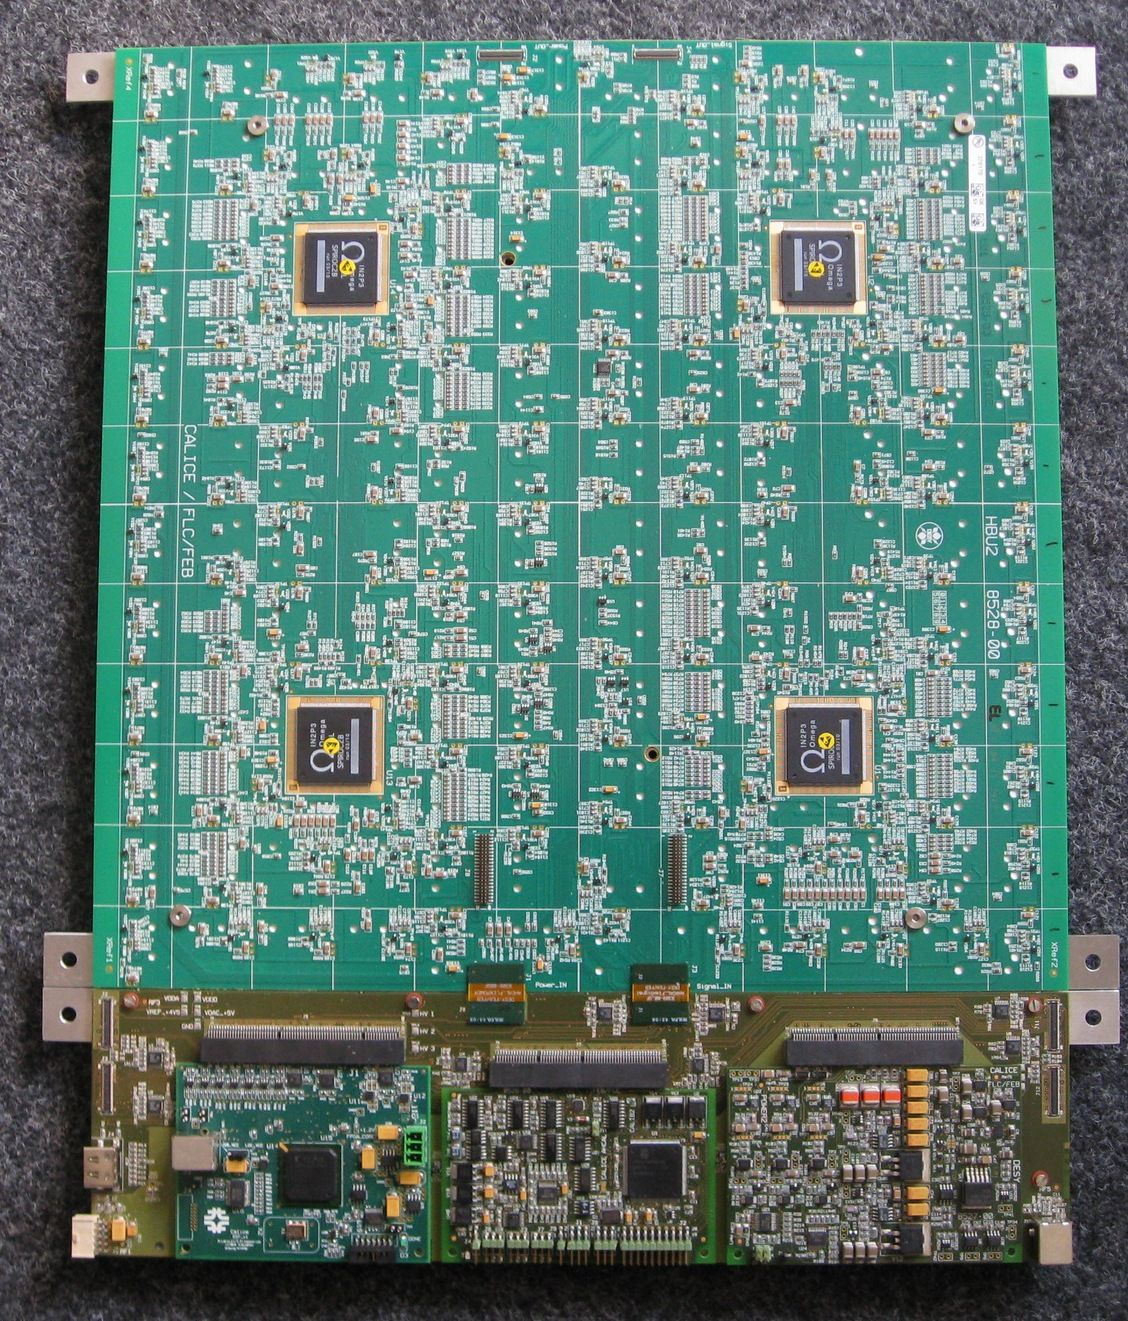
\includegraphics[width=1.\linewidth]{chap3/fig/CALICE_AHCAL_20120323.jpg}
    \caption{} \label{fig:AHCALHBU}
  \end{subfigure}
  \hfill
  \begin{subfigure}[t]{0.61\textwidth}
    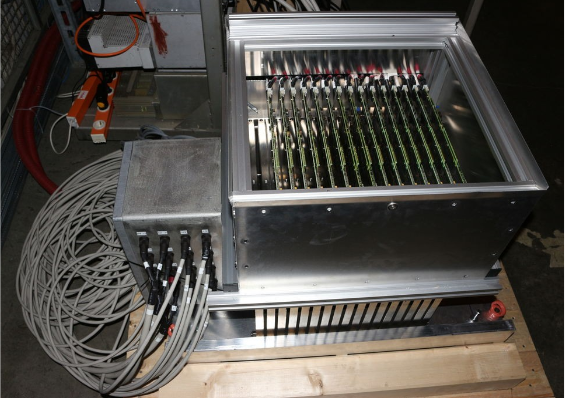
\includegraphics[width=1.\linewidth]{chap3/fig/small_HCAL_stack.png}
    \caption{} \label{fig:AHCALSmallStack}
  \end{subfigure}
  \caption{\subref{fig:AHCALHBU}) Top view of the HBU2 with SPIROC2b. \subref{fig:AHCALSmallStack}) Photo of the small AHCAL stack operated at CERN in June 2017.}
\end{figure}

A first milestone has been achieved by the construction of the small prototype of 15 AHCAL layers in 2016, see figure \ref{fig:AHCALSmallStack}. The goals for this prototype are the further validation of the surface mounted tile-SiPM design using Hamamatsu MPPCs with 2700 px and the new HBU (version 4) design, the performance of such calorimeter in electron beams at DESY, the operation in power-pulsing mode and in magnetic field \cite{CR_IEEE2017}. Moreover, this prototype has been used as backing calorimeter for the CMS HG-HCAL prototype for the HL-LHC upgrade \cite{Felix:AHCALMain2017_HGHCAL}.

Concerning the assembly of HBU boards, for electric components, this is fully automatized. For the scintillator tiles, the assembly on a mass-production scale is being investigated and is currently being demonstrated for the production batch of HBU boards \cite{Phi:AHCALMain2017}.

The current AHCAL DAQ system is fully capable of operating a full scale calorimeter prototype in testbeam in various configurations and is being extended to integrate with other DAQ systems of other detectors (CMS HG-HCAL prototype, Sc/SiECAL prototype...) and testbeam instrumentation (Telescope, Trigger Logic Unit (TLU)...) using the common EUDAQ framework \cite{Kvasnicka:CR_IEEE2016, Kvasnicka:2017bpx, Wing:2296332}.

Over the last years, several iterations of the SPIROC2 ASIC have been designed, produced and tested (SPIROC2 up to SPIROC2d). However, issues have been showed for all iterations which limit their use in testbeams. A next iteration, the SPIROC2e is supposed to correct all known problems of the previous iterations and also is the first SPIROC version to use Ball Grid Array (BGA) as packaging.

\begin{figure}[htbp!]
  \centering
  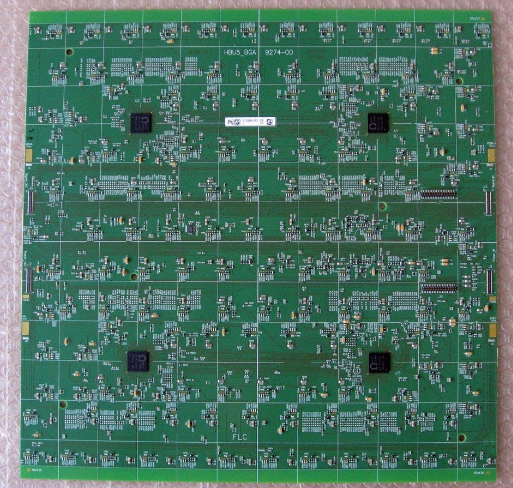
\includegraphics[width=0.45\linewidth]{chap3/fig/HBU5_BGA.png}
  \caption{Photo of the top view of the HBU5 with SPIROC2e used for the new AHCAL prototype.} \label{fig:HBU5_BGA}
\end{figure}

The next milestone is the construction and operation of a full calorimeter prototype consisted of 40 $2\times2$ HBU layers equipped with the current surface-mounted MPPCs and tiles, in a steel absorber stack and using the SPIROC2e as front-end electronics, see figure \ref{fig:HBU5_BGA}. It is planned to be operated in power-pulsing mode in various electron and hadron beams at CERN in 2018 before the shutdown \cite{Felix:AHCALMain2017}.

\subsection{SDHCAL}

The Semi-Digital Hadron Calorimeter (SDHCAL) prototype (see figure \ref{fig:SDHCAL}) consists of 48 active layers. Each active layer consists of 2-glass Resistive Plate Chambers (RPCs) \cite{BEDJIDIAN2010120} with a gap of 1.2 mm filled with gas and a readout electrode segmented in $1\times1$ cm$^2$ pads. The active layers are inserted into a steel absorber structure of 1.5 cm thick plates. The gas mixture consists of Forane (93\%), CO$_2$ (5\%) and SF$_6$ (2\%). A high voltage of around 7 kV is applied to the RPCs. The detection principle of such calorimeter is based on gas ionization and avalanche multiplication and more details can be found in \cite{1748-0221-10-10-P10039}.

\begin{figure}[htbp!]
  \centering
  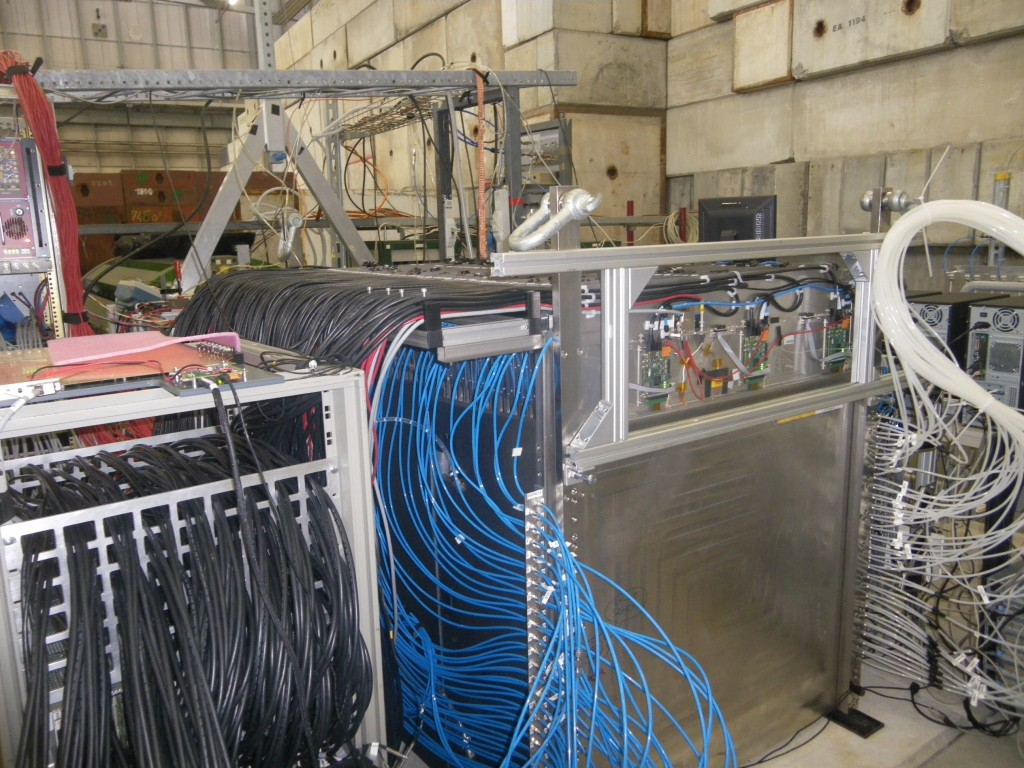
\includegraphics[width=0.7\linewidth]{chap3/fig/SDHCAL.jpg}
  \caption{Photo of SDHCAL at CERN in 2012.} \label{fig:SDHCAL}
\end{figure}

The readout is performed by the HARDROC ASIC \cite{HARDROC:IEEE} which can readout up to 64 channels. Three thresholds are used for the readout. These are not to estimate the deposited energy in a cell, it is possible but only with a large error due to large fluctuations in the avalanche process, but rather to distinguish if the recorded charge is the results of one, few or many particles traversing one cell.

The energy reconstruction of the SDHCAL is based on the information provided by the 3 thresholds. The energy is then reconstructed as a weighted sum of the number of hits for the 3 thresholds as follows:
\begin{equation}
  E_{rec} = \alpha N_1 + \beta N_2 + \gamma N_3
\end{equation}
where N$_1$, N$_2$ and N$_3$ are the number of hits for each thresholds and $\alpha$, $\beta$, $\gamma$ the weights in units of GeV. The weights are parametrized as a second order polynomial of the total number of hits N$_{hits}$ =  N$_1$ + N$_2$ + N$_3$.

\subsection{DHCAL}

The Digital Hadron Calorimeter prototype is a sampling calorimeter consisted of 38 active layers. Each active layer consists of 3 GRPCs stacked to form an active area of $1\times1$ m$^2$. The chambers are in a cassette with a front copper plate 2 mm thick and back steel plate 2mm thick. They are inserted into a steel absorber structure into gaps 1.4 cm wide. A schematic of the cross-section of a DHCAL layer is shown in figure \ref{fig:DHCALCross}. The gas mixture used is similar than for the SDHCAL with slight variations in concentrations. The readout anode is segmented into $1\times1$ cm$^2$ pads, read out by 2 front-end boards for each RPC (a total of 6 boards for a layer) hosting 24 chips each for a total of 144 chips per layer. Each chip reads out 64 pads. The prototype accounts for a total of 350208 channels.

\begin{figure}[htbp!]
  \centering
  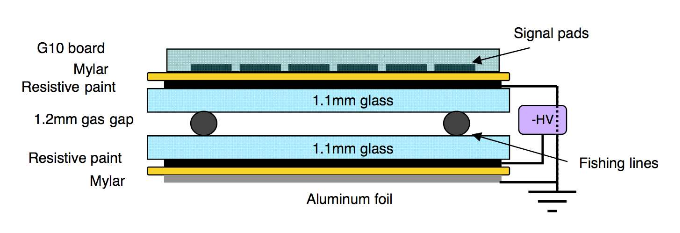
\includegraphics[width=0.9\linewidth]{chap3/fig/Cross-section-DHCAL.png}
  \caption{Cross-section of an active RPC layer in the DHCAL prototype. Taken from \cite{1748-0221-3-05-P05001}.} \label{fig:DHCALCross}
\end{figure}

The detection principle is the same followed by the SDHCAL with the main difference being in the readout of the pads. The measured charged is not proportional to the original deposited energy, the signal pads are read out in 1 bit (on or off). Each chip thus gives a hit pattern of 64 bits with a timestamp per hit of a resolution of 100 ns. More details about the DHCAL prototype can be read in \cite{Neubueser2016}.

\begin{center}
\rule{0.5\textwidth}{.4pt}
\end{center}

In this chapter, the calorimeter concepts (electromagnetic and hadronic) of the CALICE Collaboration have been described. Concerning the hadronic calorimeters, 3 concepts have been presented. The AHCAL uses scintillator-tiles coupled to a SiPM readout system to measure the deposited energy in each cell. The DHCAL and SDHCAL use resistive plate chambers by ionization of a gas mixture and avalanche multiplication to measure a signal and are readout on 1 or 3 bits by measuring the number of hits. A detailed comparison study of these different calorimeter concepts has been done and can be read in \cite{Neubueser2016}.


%%% AHCAL Commissioning, Noise Measurement and Simulations %%%
%!TEX root = ../main.tex
\chapter{\geant Simulations}
\label{chap:G4Simulation}

In High Energy Physics as well as in other research areas, simulations are a tool that has become indispensable. They are used to provide model predictions, a guideline for an analysis as well as for optimizing cost and performance of detector designs. In this thesis, the simulations will be used as a guideline for the selection of specific events of the recorded data. An understanding of their functioning is useful and will be described in this chapter.

\section{Simulation of particle showers}

The \geant framework \cite{Agostinelli2003} is a common toolkit in particle physics to simulate particle interactions with matter for a wide range of energies. Within this thesis, the simulations of CALICE calorimeter prototypes and the ILD detector concept are used in conjunction with the \mokka \cite{Freitas2003} and \ddhep \cite{Frank2014} framework. These frameworks provide a variety of tools for the implementation of detector geometries. \geant offers various tools and models to simulate physics processes in particle showers.

\subsection{Electromagnetic shower models}

Electromagnetic showers are generally well understood. This is mainly due to the fact that only electrons, positrons and photons are involved and their interaction with matter is simple as described in section \ref{subsec:PartInter}. All EM interactions are simulated with a standard EM package in \geant \cite{Ivanchenko2010}. This package has been extensively compared to many observables measured in calorimeters to a level of $\leq$ 1\% \cite{Apostolakis2015}.

Recently additions have been made to the \geant EM physics list by improving the description of ionization processes in the active medium. Then the EM list is used with a suffix \_{}EMY. This is needed in order to correctly simulate thin active layers where the detection method is very sensitive to the primary ionization, like in gas detectors such as RPCs. The use of the \_{}EMY suffix in the EM physics list is greatly improving the agreement between data and simulation in the RPC based CALICE calorimeter prototypes, the SDHCAL and DHCAL \cite{Neubueser2016}. Many other suffix options are available depending on the type of physics, detector and precision needed for EM processes.

\subsection{Hadronic shower models}

Hadronic showers are more complex in many ways than EM showers mainly due to the compositeness of the projectile as well as the target nucleus. High energy interactions between these lead to a very large phase space in the final state. The interaction is governed by the strong force and generally cannot be solved analytically. Instead, models are used using approximations and parametrizations mainly derived by theory and matched to data. Significant work has been made in the last few years in improving the modelization and accuracy of such models. The CALICE Collaboration has been of a great help in contributing to these improvements \cite{Adloff2013, Bilki2015}.

The scale of the interaction in hadronic showers is generally given by the variable $\lambda_{B} = \frac{h}{p}$ called the De Broglie wavelength. This simple variable becomes shorter as the particle energy increases thus smaller structures inside a nucleus become more relevant for the description of the interaction. \geant provides several models that are valid over various energy ranges. These models are described in the following.

\subsubsection{Intra-Nuclear Cascade Models}

For particle energies above a few hundred MeV and below a few GeV, the quark substructure of the nucleus is irrelevant. In this case, the interaction can be described by intra-nuclear cascade models (see figure \ref{fig:cascademodel}). Several models are available in \geant and will be described in the following.\\

\begin{figure}[htbp!]
  \centering
  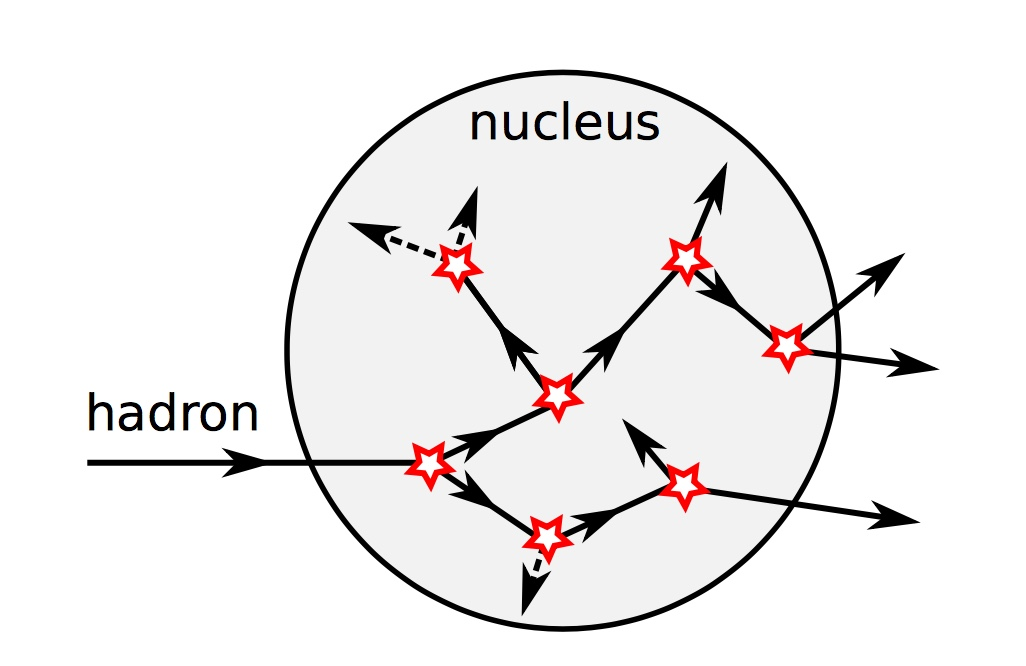
\includegraphics[width=0.5\linewidth]{chap4/fig/CascadeModel.jpeg}
  \caption{Schematic of the cascade model. The incoming projectile and all secondaries inside the nucleus are tracked and their interaction is calculated until their energy is under a certain threshold or leave the nucleus. Taken from \cite{Feege2011}.} \label{fig:cascademodel}
\end{figure}

\textbf{Bertini Cascade}\\

The Bertini cascade model \cite{Heikkinen2003} consists of the modeling of a nucleus by three concentric spherical shells of approximately constant nucleon density. The nucleons are treated as a degenerated Fermi gas in each shell and all energy levels are filled up to the Fermi energy ($E_F$). Following the Pauli exclusion principle that products can't be in an occupied state (lowest level filled by the Fermi gas), only secondary nucleons of energy $E > E_F$ can be produced. During the intra-nuclear cascade (INC), the momentum, the type of interaction and the four-momenta of the interaction for each nucleon are calculated until the energy of the tracked nucleon is below 2 MeV. The INC gives rise to excited states of the nucleus and a pre-equilibrium evaporation is computed (emission of proton and neutrons). Then a de-excitation model is applied including Fermi break-up of highly excited light nuclei (A < 12), explosion model, fission model and evaporation model until the excitation energy is below 0.1 MeV.\\

\textbf{Binary Cascade}\\

The Binary cascade \cite{Folger2004} is another approach to model the interaction between a projectile and a target nucleus. The model describes the nucleons with defined position and momentum following the nucleus mass, density distribution and Pauli's exclusion principle. The momentum is chosen randomly between zero and the Fermi momentum ($p_{F}^{max}(r)$) such that the total momentum of the nucleus is zero (at rest). The model is then treated by steps of excitations and decay into secondary particles emerging from the interaction until the average energy of all participants in the nucleus is below a given threshold (70 MeV). The remaining nucleus is further treated by pre-equilibrium and de-excitation models in \geant. The validity range of this model extends from around 100 MeV up to 10 GeV.

\subsubsection{String-Parton Cascade Models}

\begin{figure}[htbp!]
  \centering
  \begin{subfigure}[t]{0.49\textwidth}
    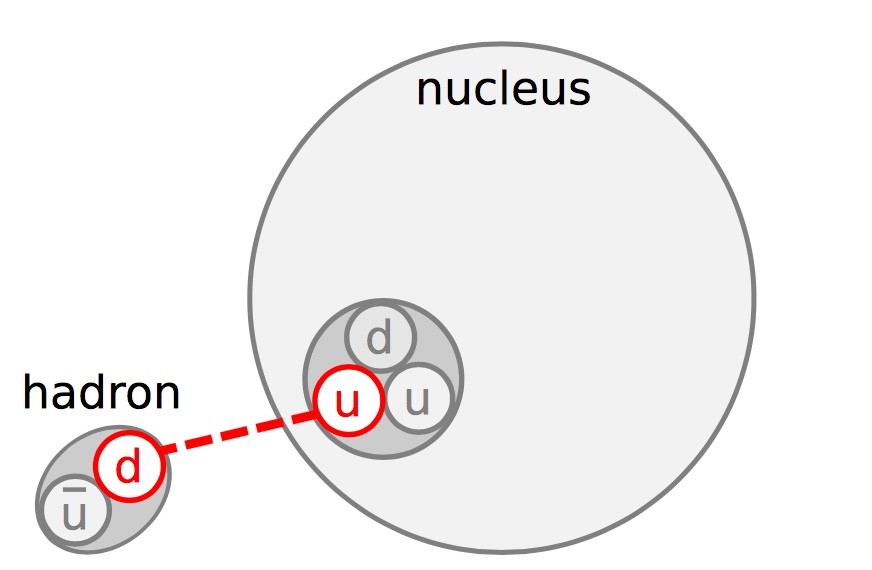
\includegraphics[width=1.\linewidth]{chap4/fig/QGS_nucleus.jpeg}
    \caption{} \label{fig:QGS_nucleus}
  \end{subfigure}
  \hfill
  \begin{subfigure}[t]{0.49\textwidth}
    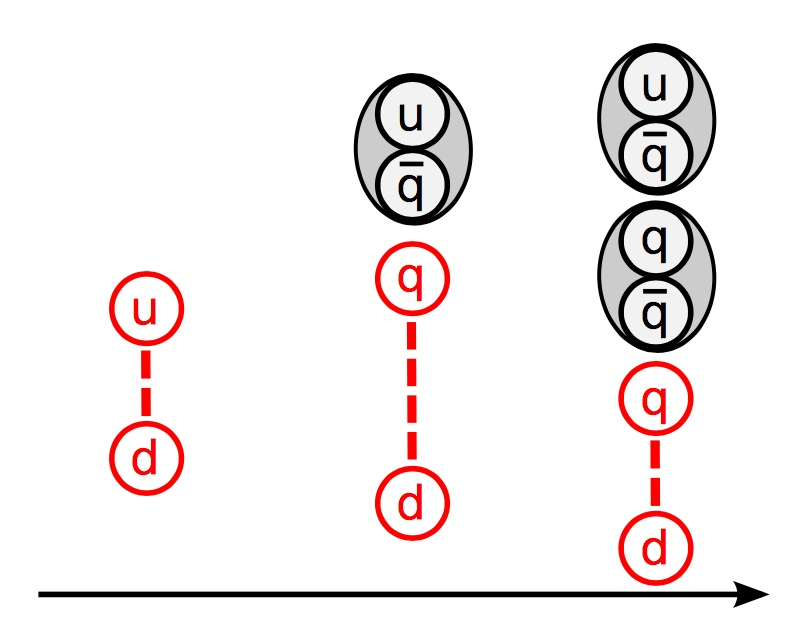
\includegraphics[width=1.\linewidth]{chap4/fig/QGS_stringfrag.jpeg}
    \caption{} \label{fig:QGS_string}
  \end{subfigure}
  \caption{\subref{fig:QGS_nucleus}) The sketch shows the formation of a string between the projectile and one of the quarks inside the nucleus. \subref{fig:QGS_string}) Representation of the fragmentation of the strings via the generation of quark-antiquark pairs into hadrons. Taken from \cite{Feege2011}.}
\end{figure}

The string-parton models \cite{Folger2003} are used in \geant to simulate inelastic scattering of particles with a target nucleus as shown in figures \ref{fig:QGS_nucleus} and \ref{fig:QGS_string}. This is used at high energies where INC models break down and where the quark substructure of the nucleons must be taken into account. The model uses string excitation to calculate the scattering. Currently, \geant provides two different models, the Fritiof model (FTF) and the quark-gluon string model (QGS).

The initial state consists of building the nucleus of individual protons and neutrons. The interaction between the primary particle and the nucleus gives place to one or more excited strings and an excited state nucleus. Quarks are the interacting constituents in the primary particle and the nucleons of the target nucleus. A string has two endpoints, such that the quark content is defined and carries energy and momentum. The fragmentation of the strings is handled by a longitudinal string fragmentation model and the interaction of secondaries is carried out by cascade models as described in the former paragraph. The de-excitation is then simulated by fragmentation, pre-compound and nuclear de-excitation models natively provided by \geant. The QGS model uses longitudinal strings to represent the momentum transfer and transverse strings for color exchange via Pomerons. In contrary, the FTF model uses an interaction probability calculated based on impact parameter, the center of mass energy, diffractive and elastic cross-sections to form a string. In the next paragraph, the QGS and FTF models are called QGSP and FTFP respectively.

\subsection{\geant Physics Lists}

\geant provides several physics lists for simulation that combine different hadron physics models. The physics lists are combinations of models, active in different energy ranges \cite{Geant4PhysicsLists:IEEE}. In this thesis, the physics lists QGSP\_BERT and QBBC are used. The validity range of the physics lists is shown in figure \ref{fig:physics_list}. The former is used in combination with the High-Precision neutron tracking (HP) package. The HP option delivers an increased accuracy in the treatment of neutron interactions below 20 MeV. The QBBC physics list includes also a tracking for neutrons with less precision than the HP package.
In addition, the QGSP\_BERT physics list uses a parametrized LEP model (based on experimental data) to fill the gap between the transition of cascade models and string-parton models.

\begin{figure}[htbp!]
  \centering
  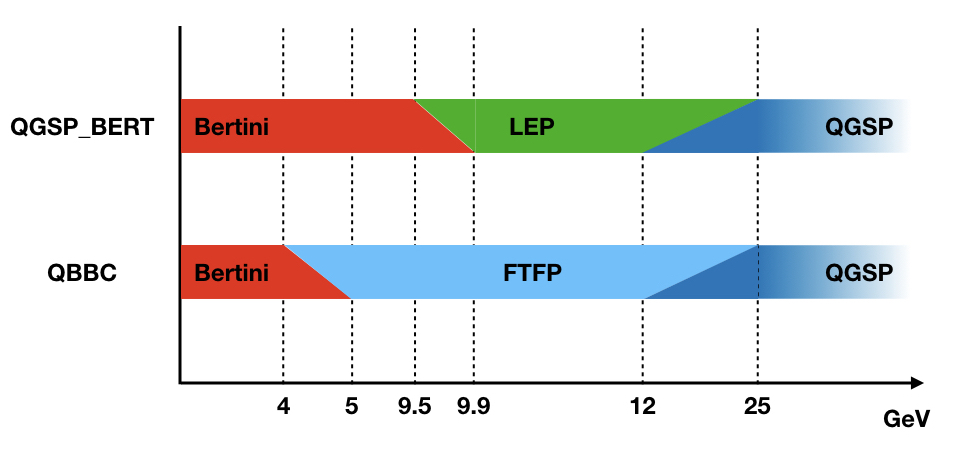
\includegraphics[width=1\linewidth]{chap4/fig/PhysicsLists.jpeg}
  \caption{Schematic of the physics list used in \geant v10.1 for this thesis. The validity range extends above 30 GeV. The diagonal regions represent the overlap region between the different models. The probability to select each model varies linearly between 0 and 100\% in the overlap region.} \label{fig:physics_list}
\end{figure}

\section{AHCAL Detector Geometry implementation and Digitization}

\subsection{Geometry implementation}

The simulation of the testbeam prototype is based on the \mokka framework v08-05-01 and the new \ddhep framework v00-16, which both provide a full \geant v10.1 based simulation of the detector with detailed geometry and material descriptions. A right-handed coordinate system is used such that the Z-axis points in the beam direction and that the Y-axis is directed upwards. No beamline instrumentation is simulated except scintillator triggers in front of and behind the detector. An additional layer of 5.6 mm of lead (corresponds to 1 $X_0$) is added in front of the calorimeter in order to account for missing upstream material. This additional material was determined using the electron data and matching the simulation with the center of gravity distribution in the z-direction (see appendix \ref{appendix:SimulationVal}).

This analysis uses the sub-detector \mokka models \textit{TBecal4d} for the ScECAL (Scintillator strips with EBUs) and \textit{TBhcal4d} for the AHCAL. The distance between the sub-detectors is set to 0 mm. The absorber structure is square-shaped in simulation, on contrary wedge-shape in reality, but it is not expected to have any influence. The placement of the active layers are the following: 2 single EBU boards, 8 single HBU boards and 4 $2\times2$ HBU boards (in slots 11, 13, 21, 31 of the absorber structure). A schematic can be seen in figure \ref{fig:Det_layout}.
\begin{figure}[htbp!]
  \centering
  \begin{subfigure}[t]{0.59\textwidth}
    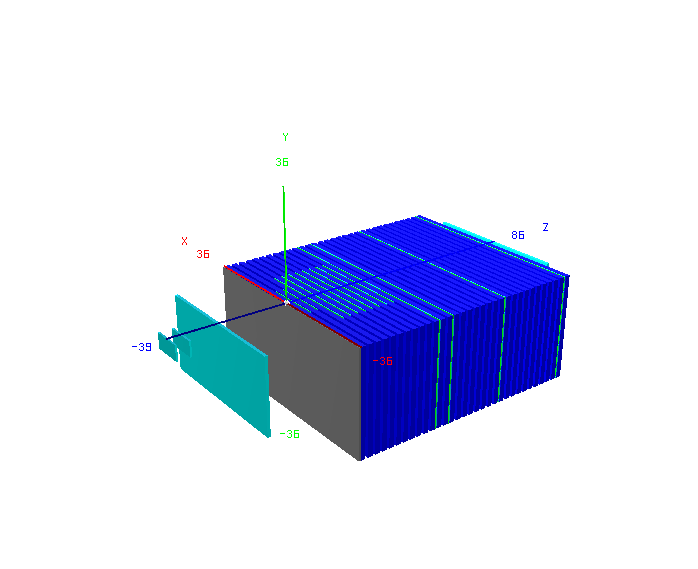
\includegraphics[width=1.\linewidth]{chap4/fig/DD4hep_AHCALModel.png}
    \caption{} \label{fig:GeomModel}
  \end{subfigure}
  \hfill
  \begin{subfigure}[t]{0.39\textwidth}
    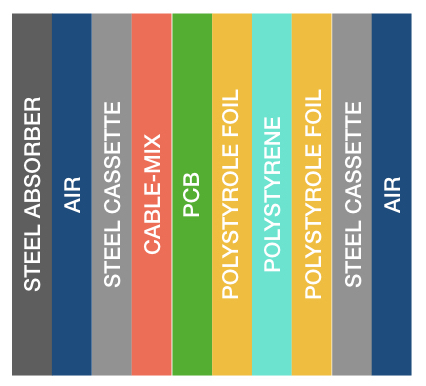
\includegraphics[width=1.\linewidth]{chap4/fig/Structure.jpeg}
    \caption{} \label{fig:material_layout}
  \end{subfigure}
  \caption{\subref{fig:GeomModel}) DD4hep geometry model of the 2015 testbeam prototype. The dark blue represents the steel absorber structure, the light blue represents the active scintillator layers and the beam instrumentation in front and back of the calorimeter and the dark grey represents the additional lead material to account for missing upstream material. \subref{fig:material_layout}) Material description of one layer in the \mokka and \ddhep simulations of the AHCAL. Dimensions are not to scale.}
\end{figure}

The material description is showed in table \ref{table:material_sim} for thicknesses and corresponding radiation length and nuclear interaction length. A schematic of the HCAL layer structure can be seen in figure \ref{fig:material_layout}. The cable-mix of 1.5 mm, the polystyrole foils of 0.115 mm and the air gaps of 1.285 mm are not listed because of the negligible impact but are present in simulations. A picture of the model in \ddhep is shown in figure \ref{fig:GeomModel}. A check was performed with \mokka and \ddhep models with muons and electrons to ensure that the material description in both models is better than 20\% (see appendix \ref{appendix:SimulationVal}).
\begin{table}[htb!]
  \centering
  \caption{Material description in \mokka and \ddhep simulations of the testbeam setup at CERN in July 2015. The X$_0$ and $\lambda_n$ numbers are obtained by the command-line \textit{materialScan} in the \ddhep framework.}
  \label{table:material_sim}
  \begin{tabular}{@{} p{6cm}|l||l|l @{}}
    \hline
    Material & thickness (mm) & X$_0$ & $\lambda_n$ \\
    \hline
    \hline
    steel absorber & 17.2 & 0.977 & 0.101\\
    \hline
    steel cassette & 0.5 & 0.028 & 0.003\\
    \hline
    PCB & 0.7 & 0.004 & 0.001\\
    \hline
    Polystyrene (ECAL/HCAL tile) & 2, 3 & 0.005, 0.007 & 0.006, 0.009\\
    \hline
    \hline
    ECAL layer & 26.2 & 1.044 & 0.115\\
    HCAL layer & 26.2 & 1.046 & 0.118\\
    \hline
    AHCAL & - & 33.24 & 3.54\\
    \hline
  \end{tabular}
\end{table}

The beam gun is placed 1 m in front of the calorimeter face for the simulations in this analysis. It is configured to generate single beam particles with a 2\% momentum spread (according to the beamline) and the beam profile for electrons and pions is extracted from data and applied to simulation. For muon runs, a flat beam covering the full AHCAL is simulated as this is not expected to have an influence on the MIP and time response of the detector. All electron simulations are simulated with \geant v10.1 using the QGSP\_BERT\_HP physics list.

Pion showers are simulated using QGSP\_BERT, QGSP\_BERT\_HP and QBBC physics lists. The package \textit{high precision} (\_HP) is used in order to understand the differences induced in timing with a precise treatment of the neutrons. The table \ref{table:event_sim} shows the number of single particle events simulated for this thesis.

\begin{table}[htb!]
  \centering
  \caption{Number of single particle events simulated in \mokka and \ddhep for each particle type and energy.}
  \label{table:event_sim}
  \begin{tabular}{@{} ccc @{}}
    \hline
    Particle & Energy & \# Events \\
    \hline
    $\mu^-$ & 150 GeV & 1 000 000 \\
    \hline
    $e^-$ & 15, 20, 30, 40 GeV & 20 000 \\
    $e^-$ & 10, 50 GeV & 200 000 \\
    \hline
    $\pi^-$ & 10, 30, 50, 70, 90 GeV & 500 000 \\
    \hline
  \end{tabular}
\end{table}

\subsection{Digitization}

The digitization of simulated hits is very similar to the one used in the ScECAL and AHCAL physics prototypes \cite{2011_JINST_6_P04003}. First, the energy deposited in a cell is converted in MIP. The conversion unit named \textit{GeVtoMIP} is extracted from simulation by projecting 8 GeV muons onto a detector tile and fitting the resulting spectrum with a Landau function. Motivated by physics, as explained in section \ref{subsec:PartInter}, ideally for a thin active material, the energy deposited follows a Landau distribution. The most probable value (MPV) of this distribution is used as the \textit{GeVtoMIP} factor. For this setup, a value of 470 keV is used for the AHCAL and 309 keV for the ScECAL.

If available, individual calibration factors obtained from data are used to extract the light yield which is needed to model the statistical fluctuations of photons hitting a SiPM \cite{Hartbrich:2016bbz}. Saturation effects are also included using the number of pixels available on each SiPM type. Most of the tiles used are wrapped with a reflective foil such that crosstalk effects between channels can be neglected. For layers with no wrapping, a default value of 15\% cross-talk is applied. Additionally, noise needs to be taken into account for the engineering AHCAL prototype. It is important to note that noise is much lower than in the physics prototype but it is important to be taken into account for this thesis as timing is very sensitive to low statistics late tails. Noise is added using muon runs by removing found tracks and keeping remaining hits. This is described in appendix \ref{appendix:noise}.

The timing is modeled in the same way as in the SPIROC, the energy from sub-hits in a cell is integrated over a sliding time window of 15 ns, if the energy sum passes the threshold, the time of the simulated sub-hit is used as the time of the hit. In order to simulate detector resolution effects, the time of a hit is smeared with a double Gaussian function with slightly different means and sigmas convoluted with a Gaussian of fixed mean and variable sigma. More details are explained in appendix \ref{appendix:ped_shift}.

After digitization, simulated hits have the same format as raw data hits and are then reconstructed using the same software chain as is used for data. To suppress noise, only hits above 0.5 MIP are considered in this analysis in both simulation and data.

\chapter{Commissioning of the AHCAL technological prototype}

Before every testbeam, all the electronics of the detector must be characterized. Before the full assembly, each individual chips must be tested in order to reject chips that presents bad channels or any other defects. After the assembly, each board needs to be characterized. This included the measurement of the SiPM-tile gain, the trigger threshold and noise. In this chapter, the testing of the chips and the commissioning procedure of the AHCAL will be presented.

\section{Testing of individual SPIROC2B chips}

The testing of individual chips prior to the soldering to the HBU board is necessary. This avoids broken chips to be installed and reduces the number of dead channels. So far, the testing had to be done manually for each chip. This reduces the number of cross-checks done on the chips due to time constrains. The SPIROC2B chip can be tested standalone on a custom made PCB board. The SPIROC2B chip is installed in a special socket and is readout out by an ALTERA FPGA. The board is operated by a Labview software made by the OMEGA group \cite{OmegaWeb}.

\begin{figure}[htbp!]
  \centering
  \begin{subfigure}[t]{0.49\textwidth}
    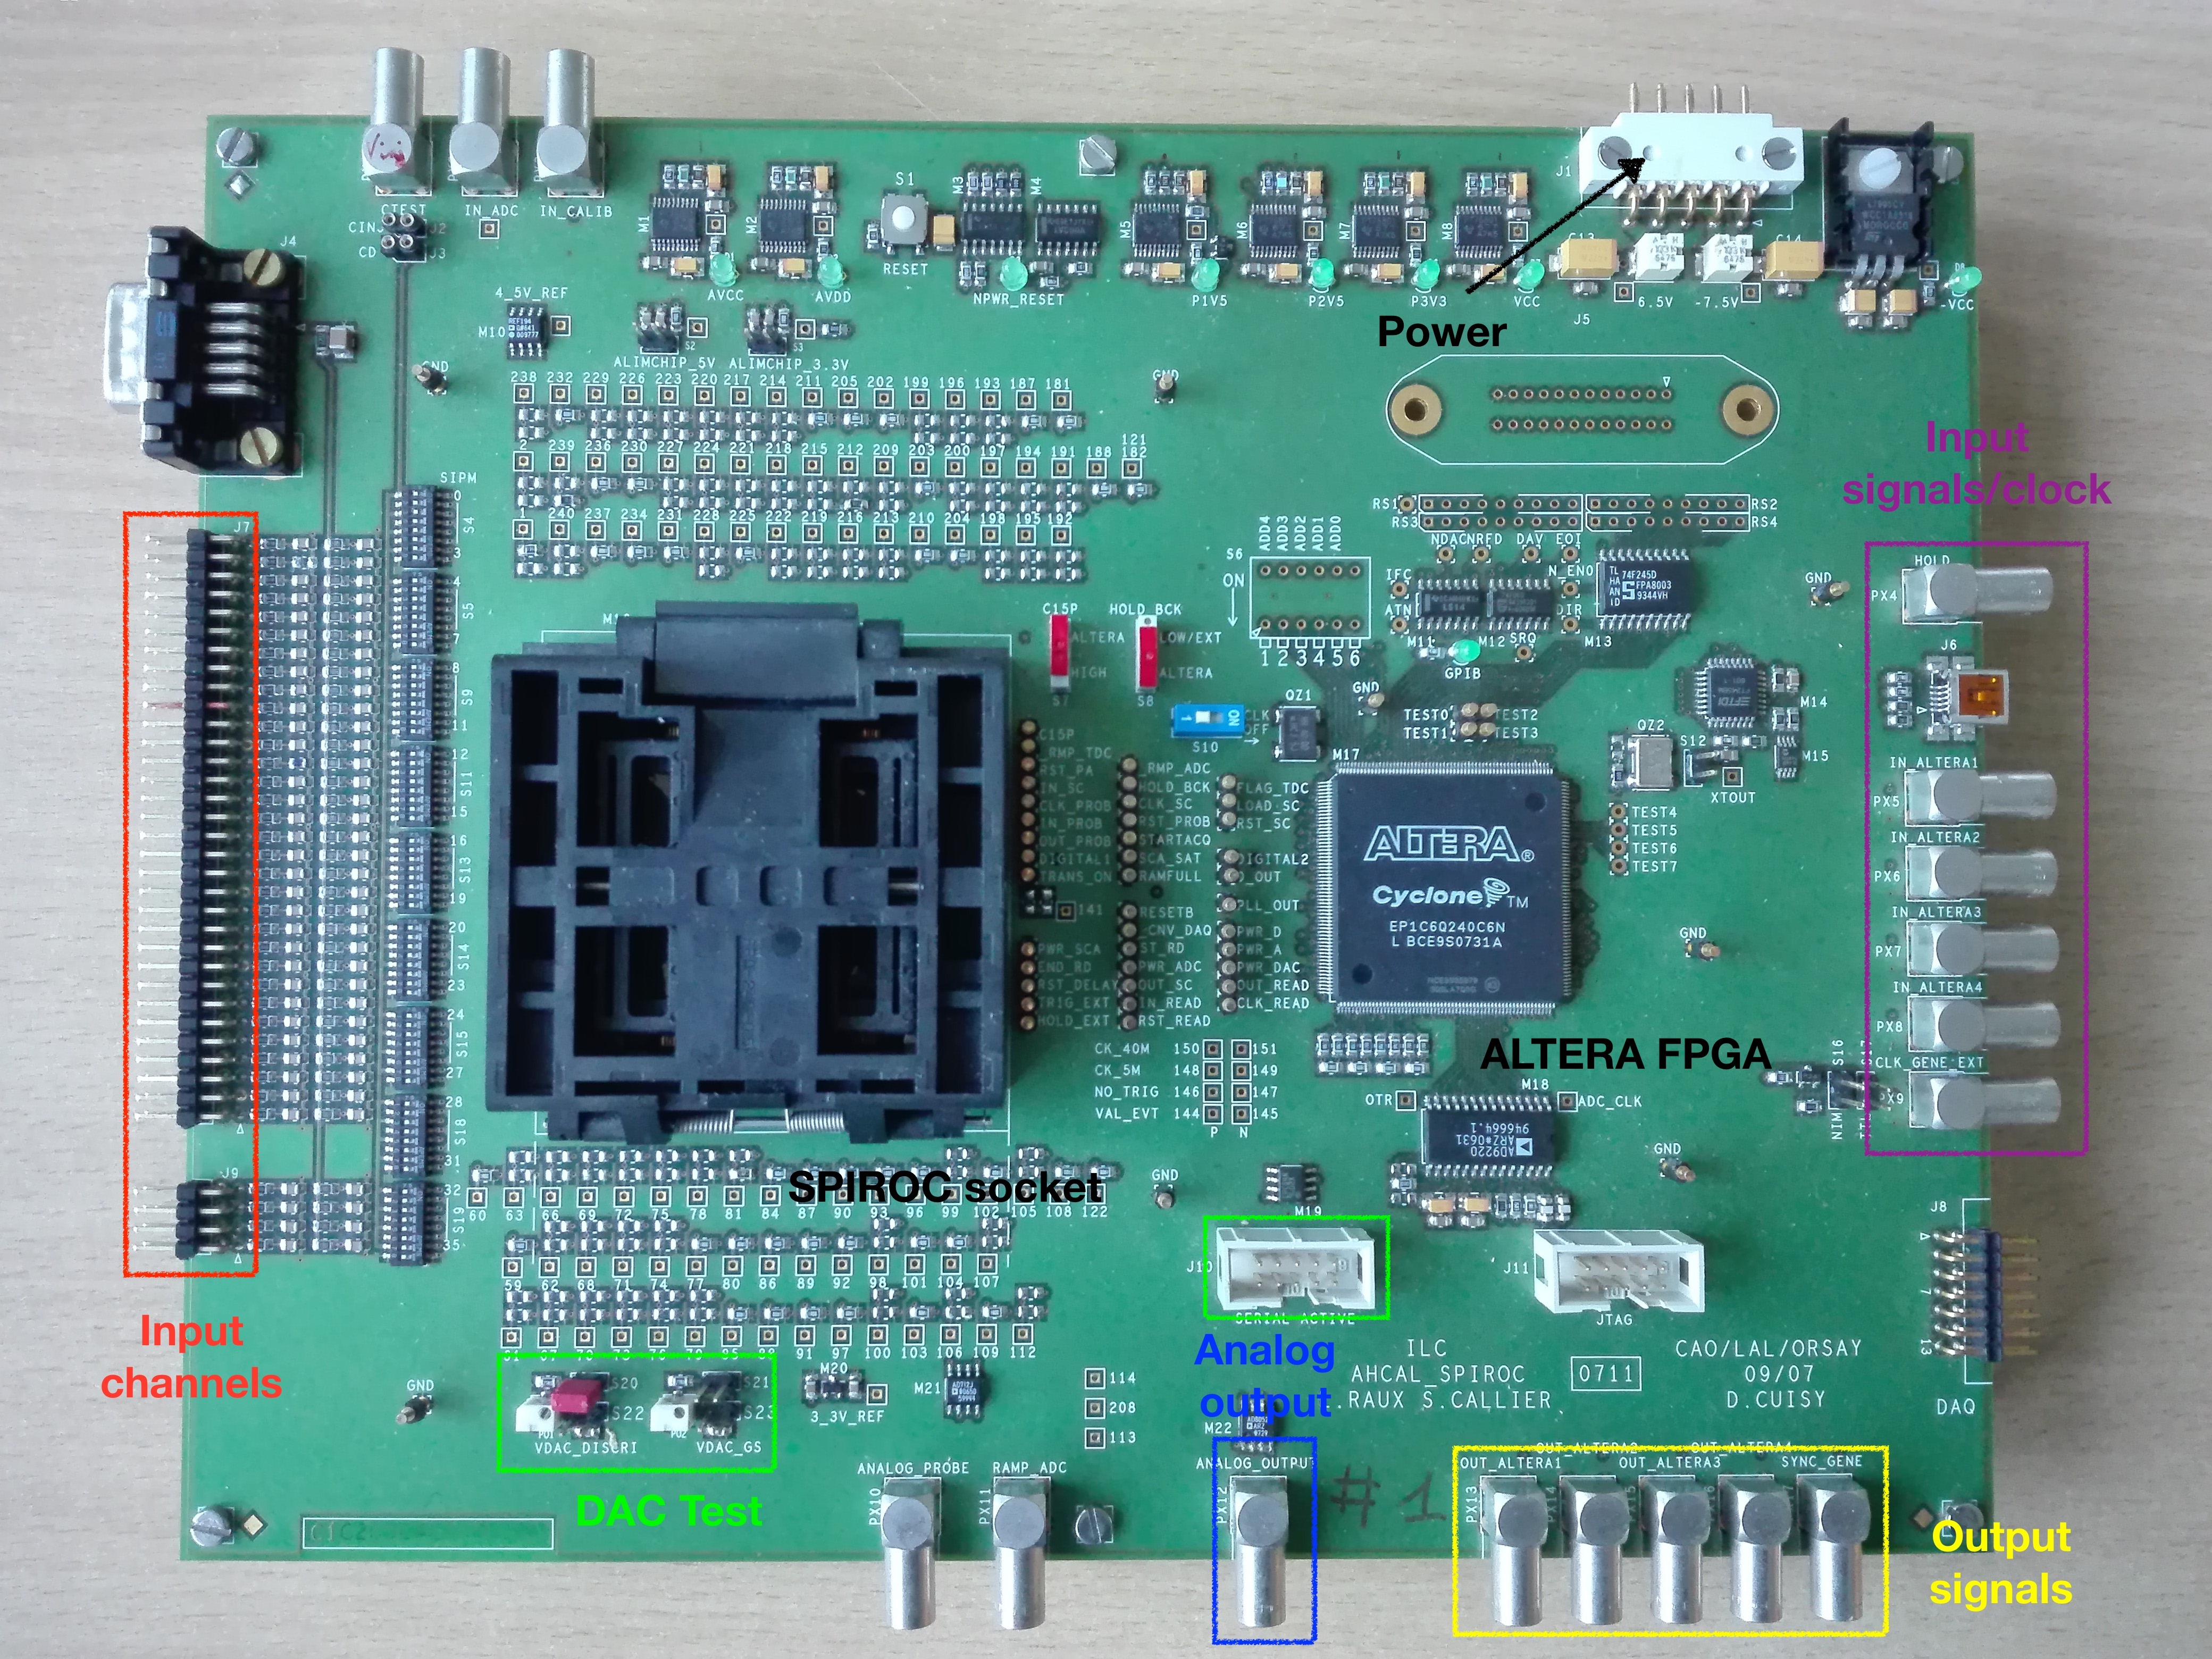
\includegraphics[width=1.\linewidth]{chap4/fig_Commi/TestBoard.jpg}
    \caption{} \label{fig:Testboard_SP2B}
  \end{subfigure}
  \hfill
  \begin{subfigure}[t]{0.49\textwidth}
    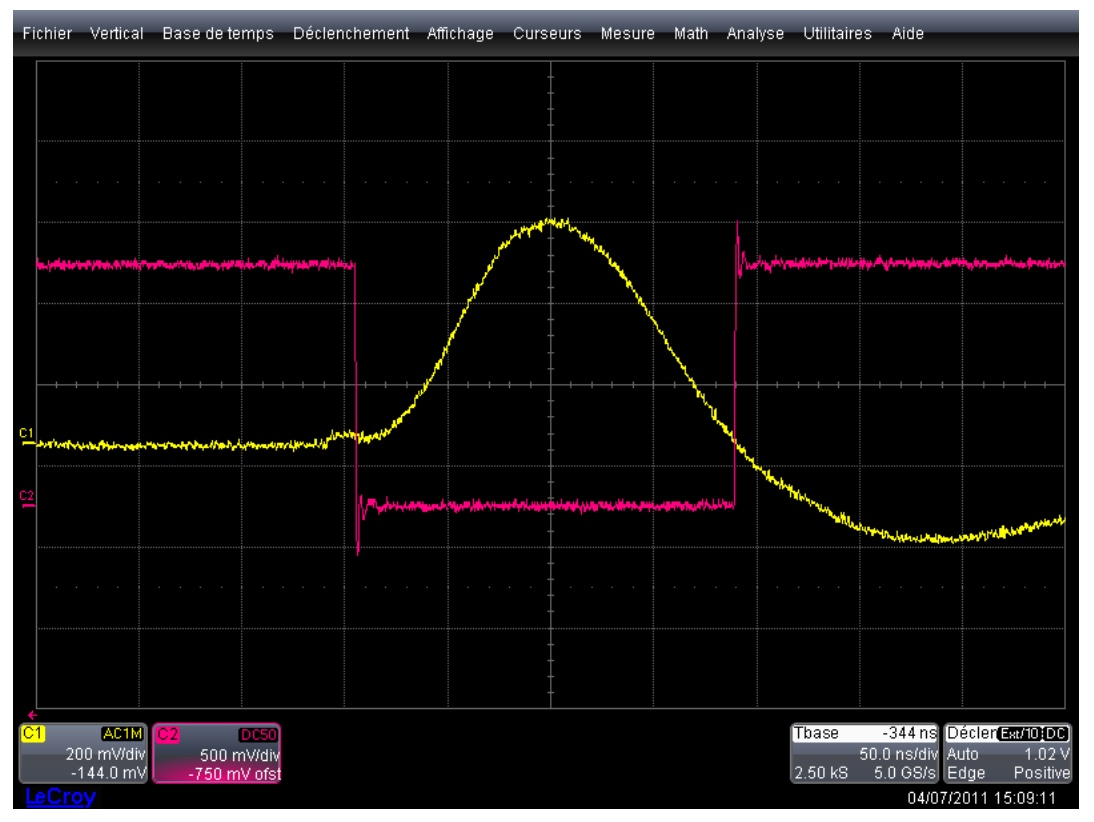
\includegraphics[width=1.\linewidth]{chap4/fig_Commi/AnalogSignalSP2B.jpeg}
    \caption{} \label{fig:AnalogSignal_SP2B}
  \end{subfigure}
  \caption{\subref{fig:Testboard_SP2B}) Testboard used to test the SPIROC2B chip standalone. \subref{fig:AnalogSignal_SP2B}) Example of an analog signal outputted by the slow shaper of the SPIROC2B. The signal is represented in yellow. The trigger is represented in red.}
\end{figure}

The board as shown in figure \ref{fig:Testboard_SP2B} contains all the debugging feature needed to check the functioning of the chip. In red, the input signal pulse, generally similar to a SiPM pulse with a fast rising edge (around 1 ns) and a slower falling edge (around 20 ns), can be injected to the 36 channels of the chip. In blue and yellow are the output signals, this enables to check via an oscilloscope the output analog signal after the slow shaper as shown in figure \ref{fig:AnalogSignal_SP2B}, but can only be checked in external trigger mode. In purple, these are the input signals for the FPGA such as the slow clock, external trigger signals. And finally in green, the DACs can be tested individually or automatically by connecting a Keithley multimeter to the serial port.

In this manual procedure, only vital parts of the chips are tested. This includes to check that all channels are working correctly, the chip works in both external and auto-trigger modes, all the DACs of the chip are working and that the digital part provides data. For the testbeam in July 2015, around 60 chips have been tested manually. The mean time for a chip to be tested was around 10 mins.

\subsection{DAC Testing}

As the testing procedure is done manually, only the most critical components of the chip needed to be tested. One of them is called the DAC which regulates the voltage channel-wise to the SiPM or the threshold discriminator. The procedure was done in two parts. First a simple check by checking the voltage on the channel at a value of 0. If one of the channel presented an unstable voltage, it indicates likely that the input DAC is broken thus the chip was discarded. If it passed, then the input DAC curve was simply measured by connecting a Keithley to the serial port and use the automatic measurement procedure from the Labview software. The time required was around 1-2 mins per chip. The output was a list containing the DAC value (from 0 to 255) and the associated voltage. The reconstructed figures are shown in \ref{fig:IDAC} for the input DAC and output DAC \ref{fig:OutDAC}.

\begin{figure}[htbp!]
  \centering
  \begin{subfigure}[t]{0.49\textwidth}
    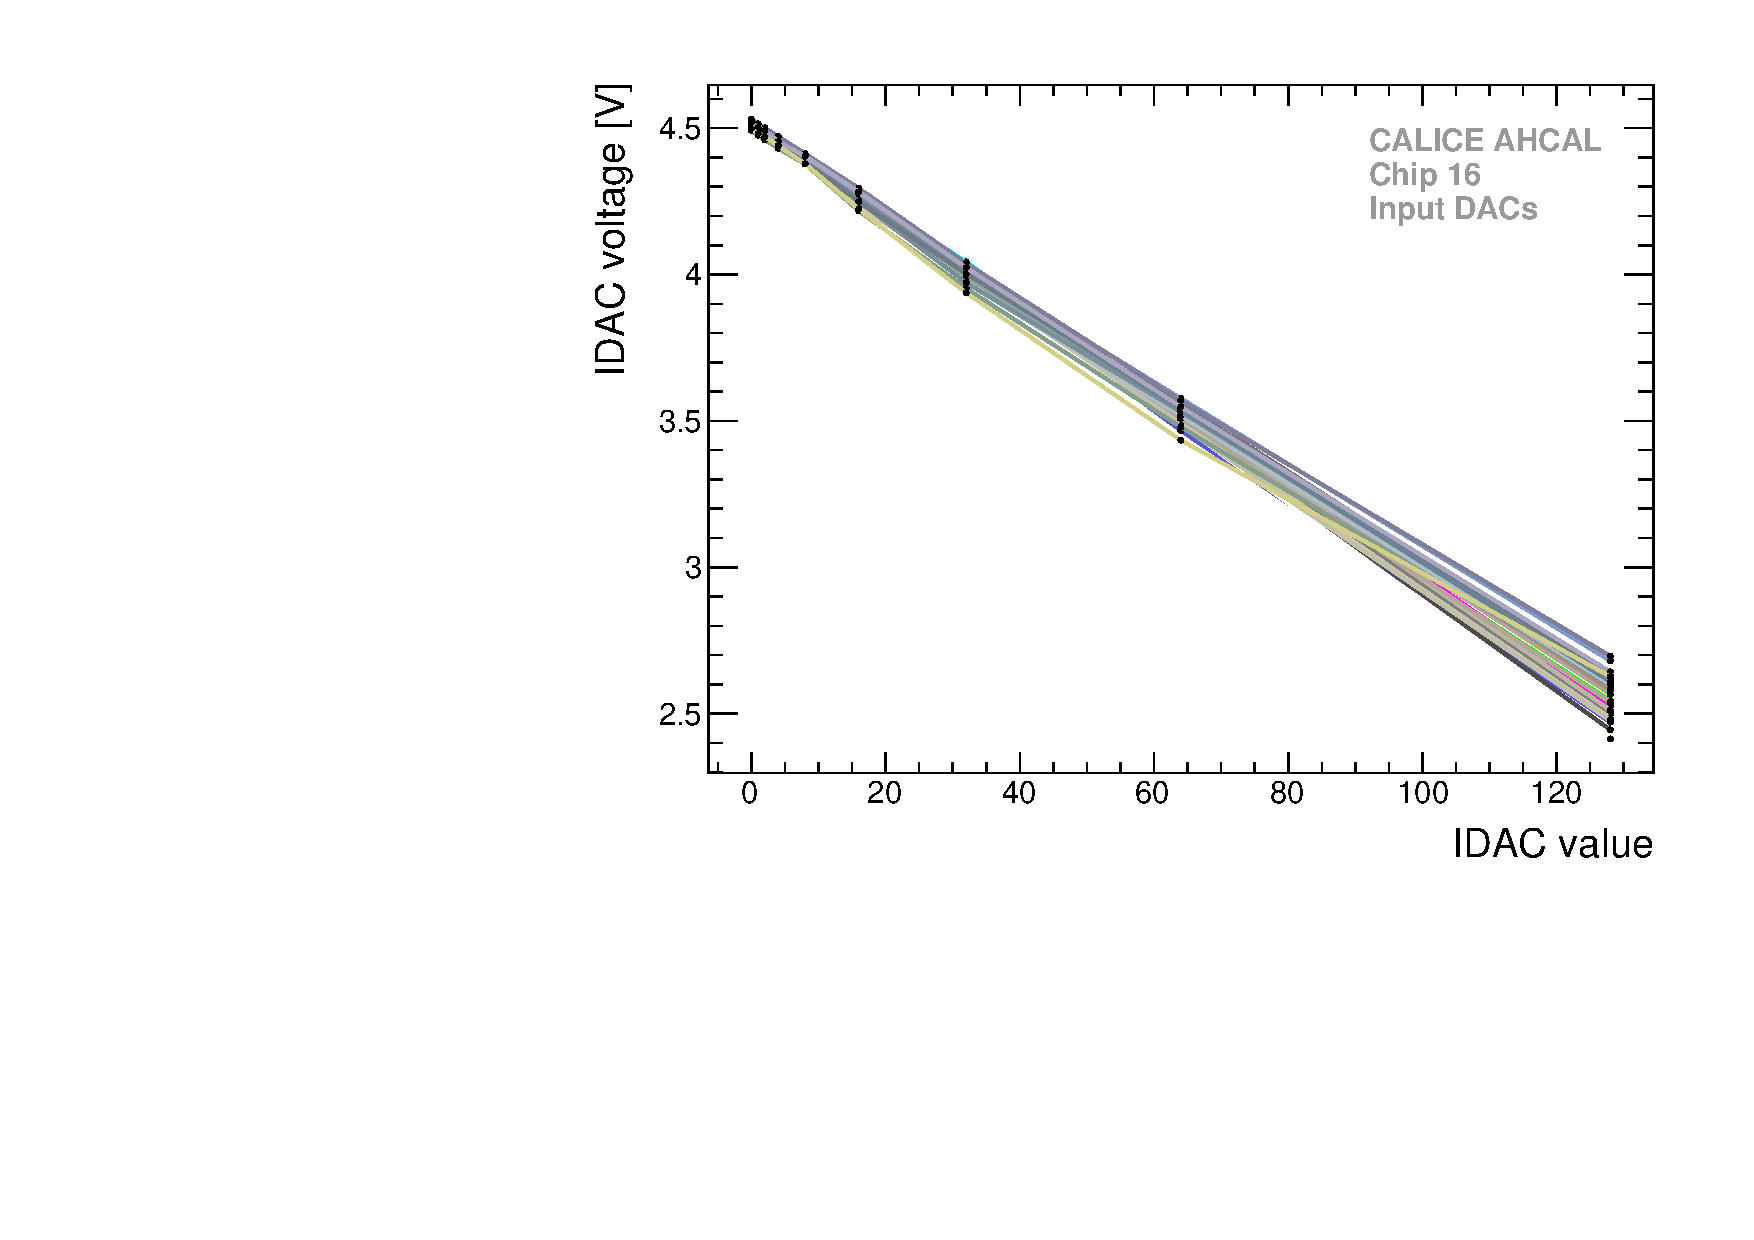
\includegraphics[width=1.\linewidth]{../Thesis_Plots/Commissioning/Plots/IDACs_Chip16.pdf}
    \caption{} \label{fig:IDAC}
  \end{subfigure}
  \hfill
  \begin{subfigure}[t]{0.49\textwidth}
    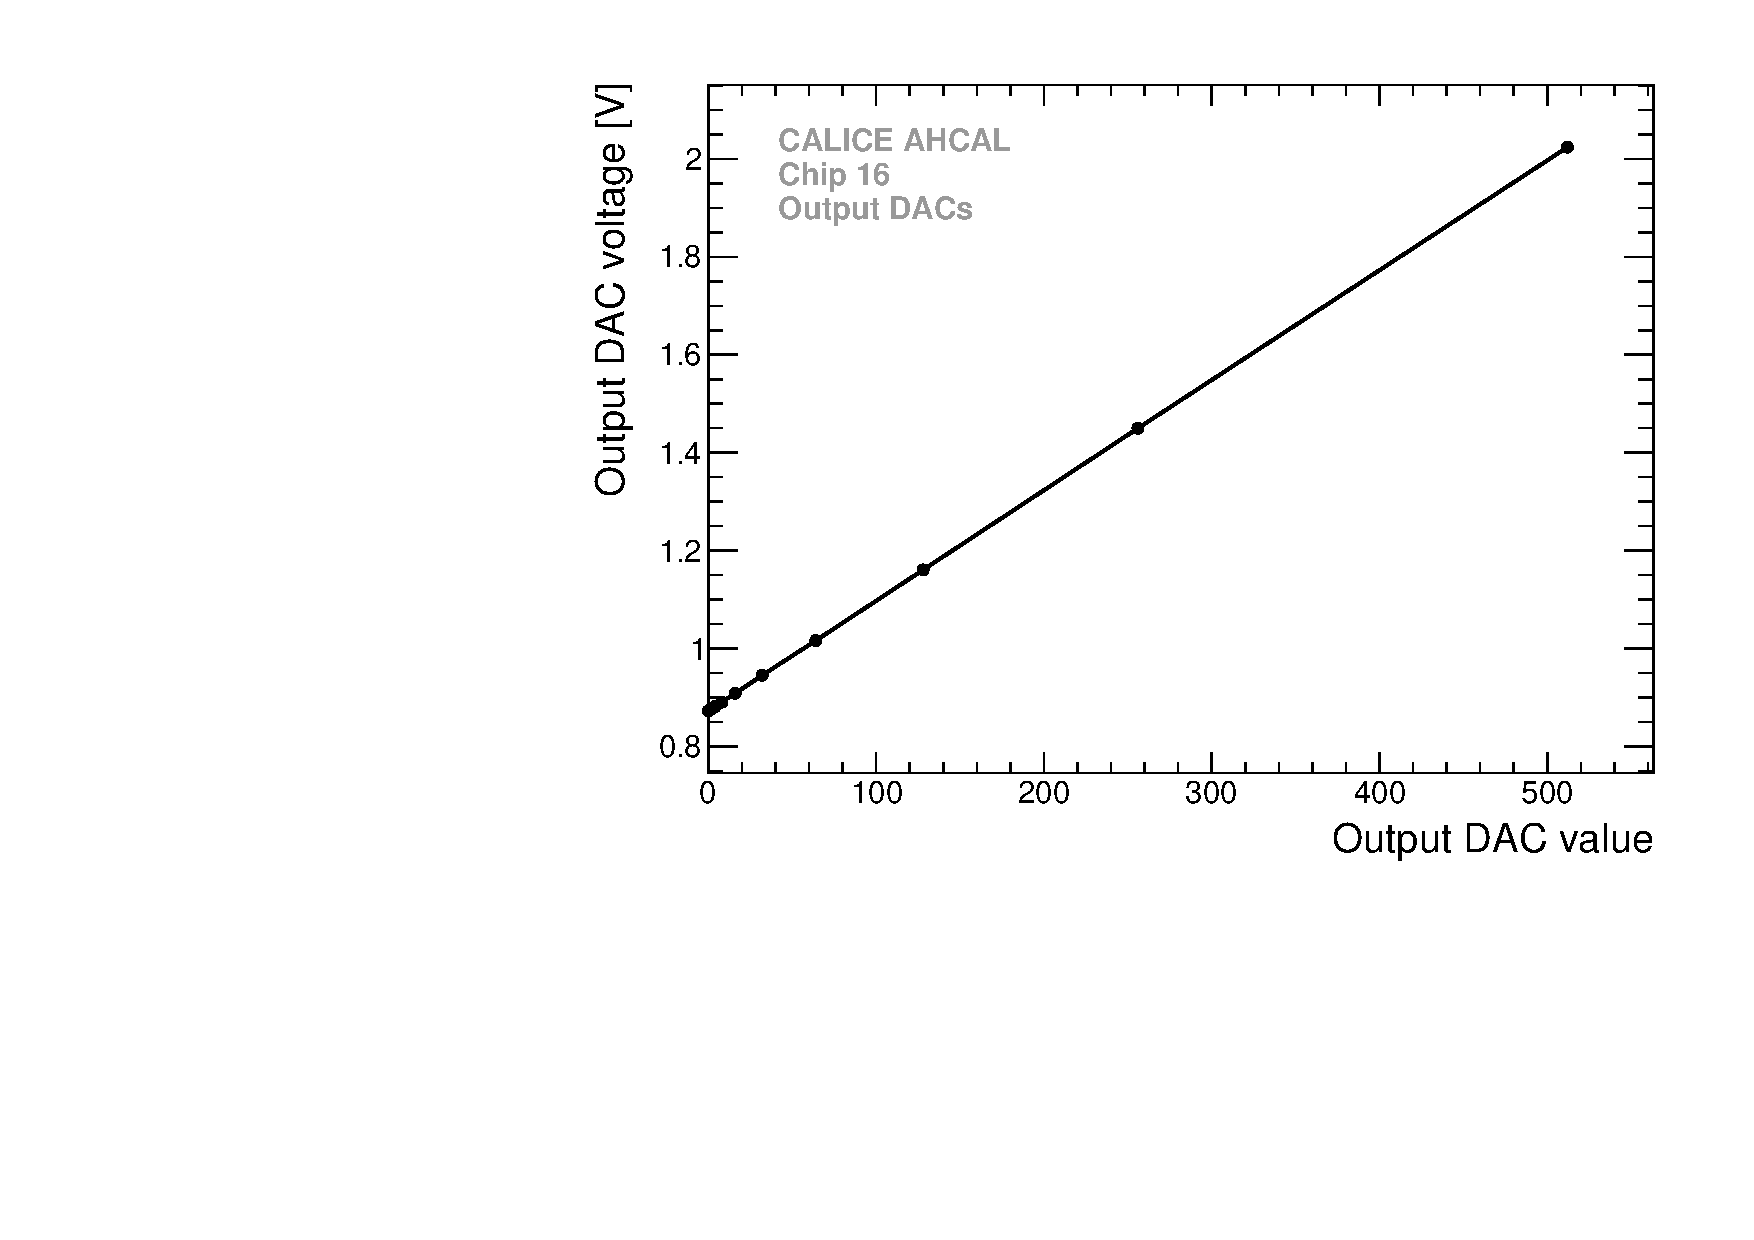
\includegraphics[width=1.\linewidth]{../Thesis_Plots/Commissioning/Plots/OutDACs_Chip16.pdf}
    \caption{} \label{fig:OutDAC}
  \end{subfigure}
  \caption{\subref{fig:IDAC}) Reconstructed input DAC curves of the 36 channels for the Chip 16 of the tested batch. \subref{fig:OutDAC}) Reconstructed output DAC curve for same tested chip.}
\end{figure}

One can notice that the spread channel-to-channel for the input DACs increases with the value. The spread is around 10 mV at a value of 0 and goes up to 200 mV at a value of 128. Thus for new produced boards, it has been chosen to use a value of 0 of the input DAC where the spread is minimal.

\begin{center}
  \rule{0.5\textwidth}{.4pt}
\end{center}

Around 60 chips were tested with a yield over 84\%. There is no obvious common cause for failure (digital part not working, no response to slow control programming, broken input DACs...). The time achieved by testing chips manually was around 10 mins which is not possible on a mass-production scale where only around 1 min is required at maximum per chip. This is why a new testing board has been designed between DESY and the University of Wuppertal in order to automatize the testing procedure of individual chips on BGA packaging \cite{AHCALMain2016_Amine}. This new board has already been commissioned in July 2017 and is being used currently for the next generation AHCAL prototype (around 650 chips).

\section{Commissioning procedure}

The commissioning procedure of the detector was done in July/August 2014 for a testbeam that was planned in October/November 2014 at the CERN PS facility. Mainly the same boards where used during the testbeams in 2015. Before the assembly of the detector into the absorber stack, each individual boards need to be tested. This test is done in order to characterize the full board assembled. The procedure is explained in details in \cite{} and was mainly done by these steps:

\begin{itemize}
  \item Setup the Power Board voltage to deliver to the SIPM and the input DAC value
  \item First Characterisation by measuring the SiPM gain at nominal settings
  \item Iterative adjustment of pre-amplifier to reach targeted SiPM gain
  \item Threshold scan measurement
  \item Noise measurement
\end{itemize}

The following subsections will describe each points into details. Only the new boards where fully commissioned. Old boards that where already calibrated used the same settings and only a cross-check was performed.

\subsection{Setting the High Voltage}

An AHCAL board or HBU is dotted of 144 channels, each equipped with a plastic tile-SiPM. To achieve a certain light yield, meaning the number of fired pixels per MIP, the SiPM must be operated above a specific voltage called the breakdown voltage ($V_{Br}$). This voltage has been measured for a couple of SiPMs but it is generally given by the manufacturer where batches of SiPM are placed in bags with a certain $V_{Br}$ and the lower/upper limits are indicated. The variation of the breakdown voltage is in the order of hundreds of millivolts. As the quality of the SiPM has increased drastically in the last few years, the need for individual channel-wise voltage is reduced. Thus the chosen input DAC value was chosen to be 0 equivalent to -4.5V on the SiPM voltage pin. Most of the SiPM are operated at 5V over the breakdown voltage but varies with the type. The needed voltage to be applied and thus delivered by the power board is given by $V_{op} [V] = V_{Br} + V_{overvoltage} + 4.5V$. The table \ref{table:Voltage_SiPM} sums up the voltages applied.

\begin{table}[htb!]
  \centering
  \caption{List of breakdown and operating voltages applied to each SiPM types.}
  \label{table:Voltage_SiPM}
  \begin{tabular}{@{} ccc @{}}
    \hline
    SiPM type \# & $V_{Br}$ & $V_{op}$ \\
    \hline
    Hamamatsu & $\sim$ 65 V & $\sim$ 70 V \\
    CPTA & $\sim$ 35-45 V & $\sim$ 37-50 V \\
    Ketek & $\sim$ 28 V & $\sim$ 32 V \\
    UHH Ketek & $\sim$ 27 V & $\sim$ 30 V \\
    SenSL & $\sim$ 26 V & $\sim$ 30 V \\
    \hline
  \end{tabular}
\end{table}

\subsection{First Characterization of the gain}

In this section, the SiPM gain is related to the ADC value between two peaks of a single pixel spectra where individual pixels, in a relative small number (~10-15 pixels), are fired by an integrated LED system. This value is proportional to the high voltage applied to the SiPM and can be also modified by adjusting a feedback capacitor to the SPIROC2B high gain pre-amplifier. Before starting the gain measurement procedure, a holdscan needs to be performed. This procedure determines the necessary Hold time bits to set in the slow control configuration to sample the maximum of the signal. The procedure is simple, a fixed amplitude signal is injected via the LED integrated system to all the channels while repeating this for several Hold time values. The analysis enables to reconstruct the signal shape after the slow shaper and thus determine the Hold time necessary per chip as shown in figure \ref{fig:Holdscan}.

\begin{figure}[htbp!]
  \centering
  \begin{subfigure}[t]{0.49\textwidth}
    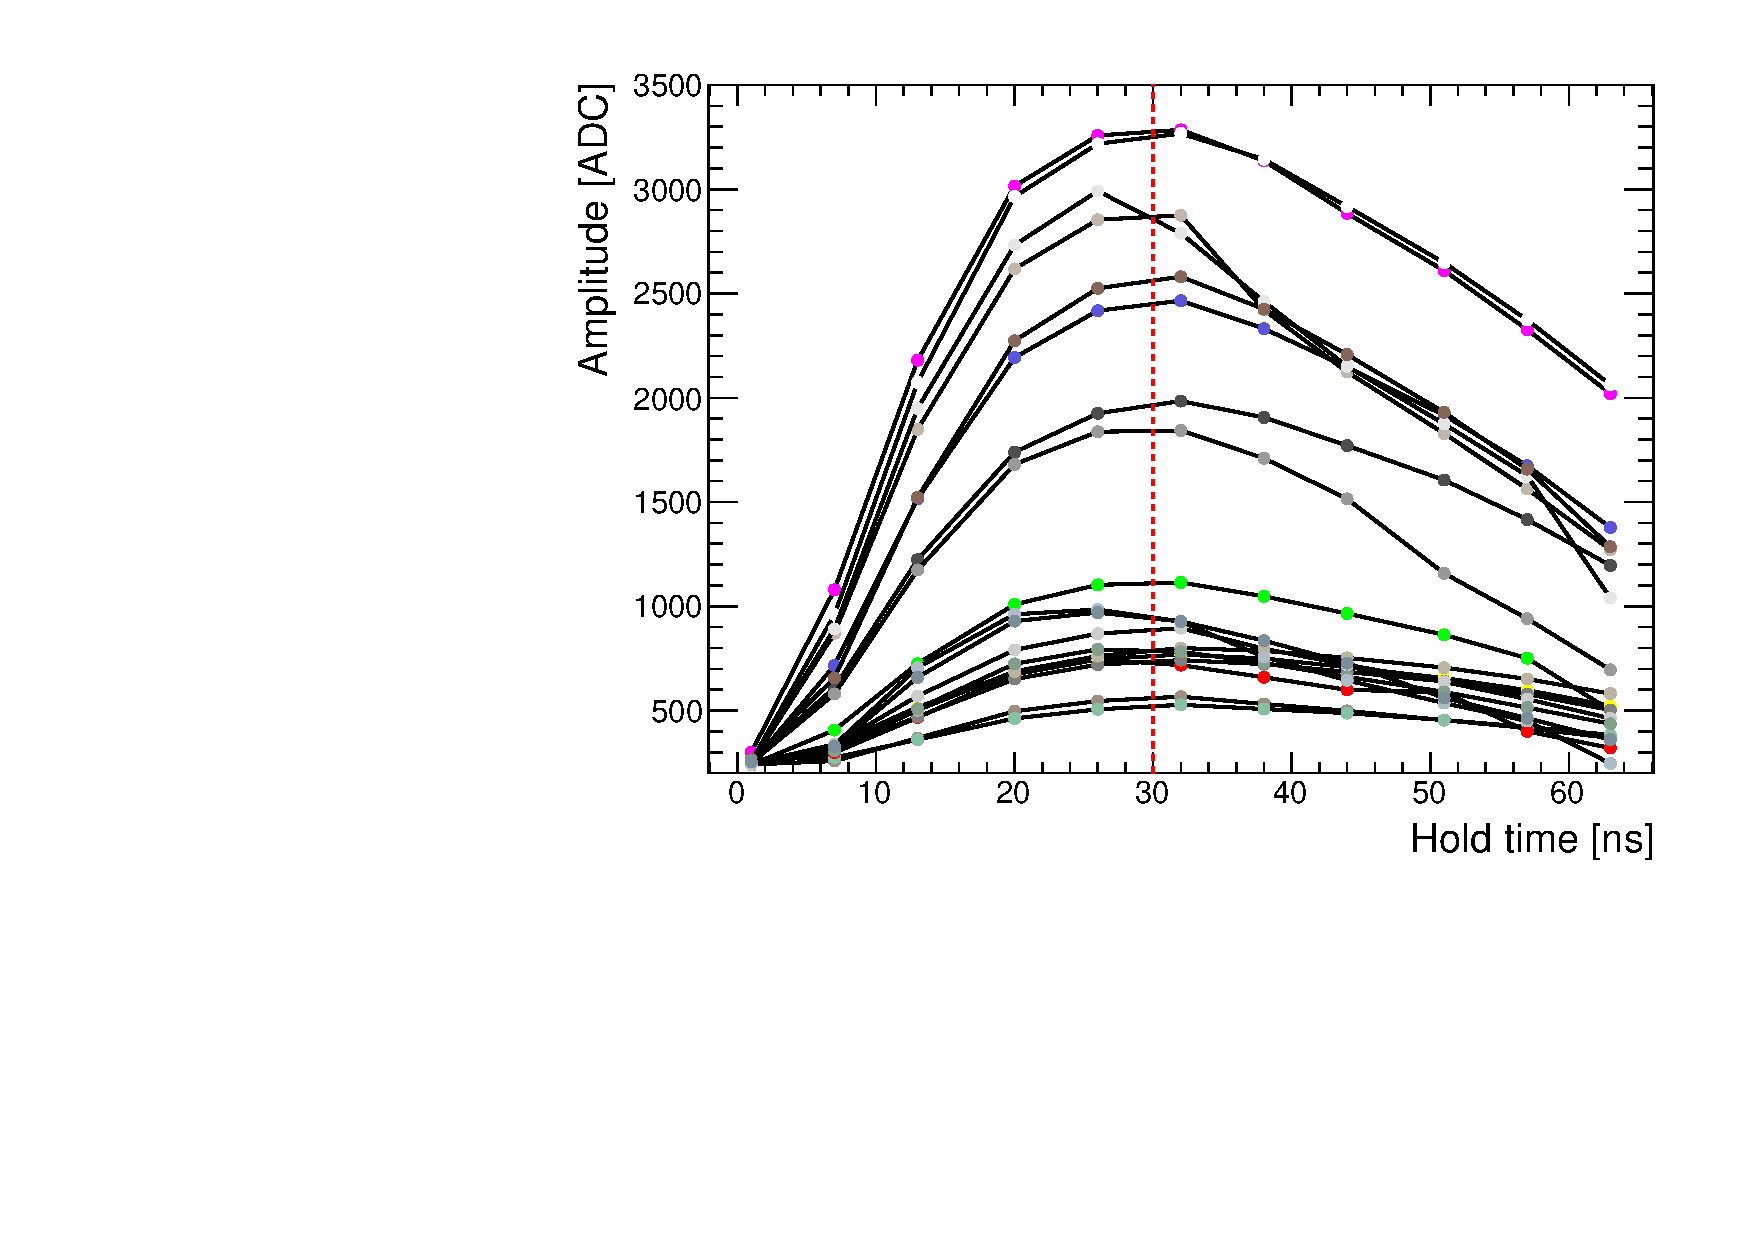
\includegraphics[width=1.\linewidth]{../Thesis_Plots/Commissioning/Plots/Holdscan_HBU2_15.pdf}
    \caption{Holdscan} \label{fig:Holdscan}
  \end{subfigure}
  \hfill
  \begin{subfigure}[t]{0.49\textwidth}
    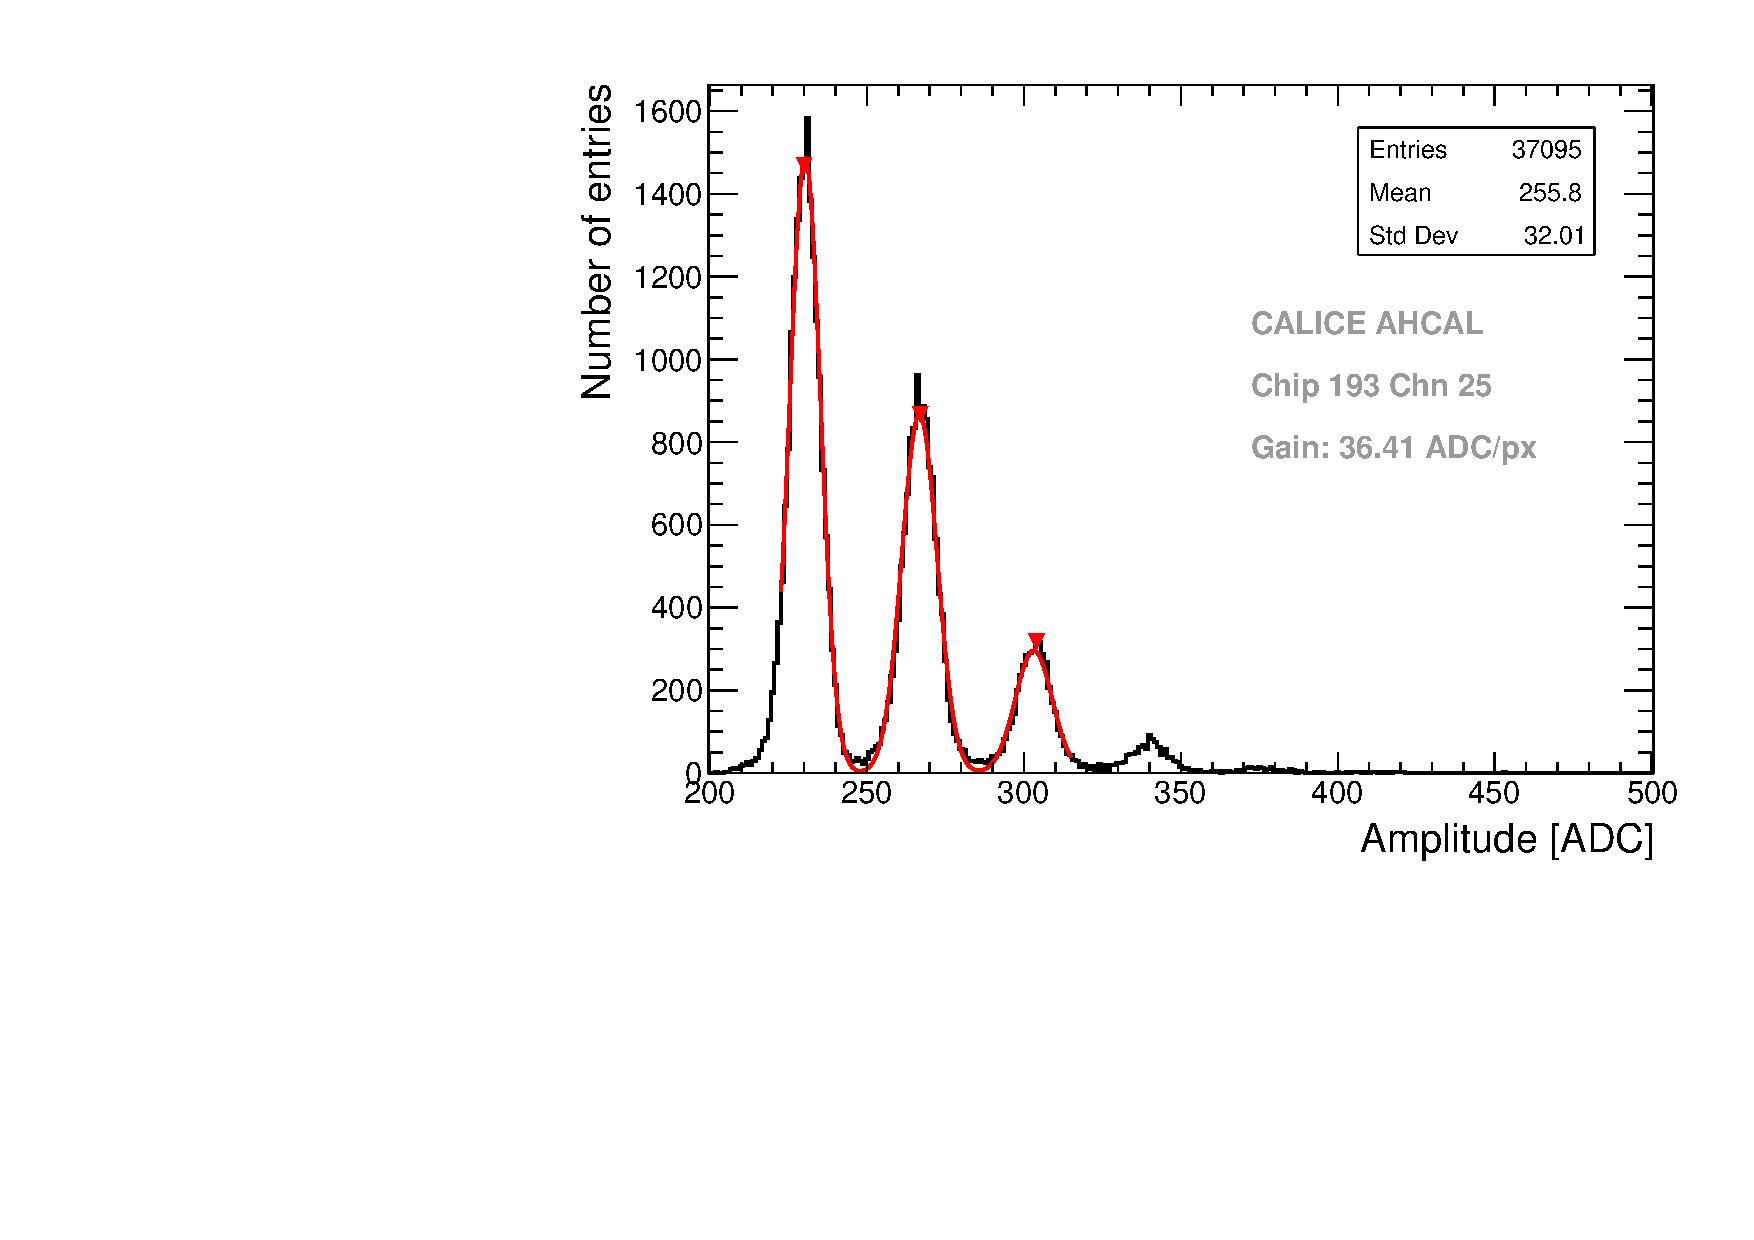
\includegraphics[width=1.\linewidth]{../Thesis_Plots/Commissioning/Plots/Gain100fF_MainzHBU4.pdf}
    \caption{Gain measured at 100 fF} \label{fig:Gain100fF}
  \end{subfigure}
  \caption{\subref{fig:Holdscan}) Reconstructed signal shape for several channels. The dotted red line represent the Hold time chosen for this board. \subref{fig:Gain100fF}) Single pixel spectra of a single channel. The fit is done by a Multi-Gaussian where the distance between the 1$^{st}$ and 2$^{nd}$ peaks is the fitted SiPM gain.}
\end{figure}

After this, a first characterization of the gain can be done at nominal settings which is using a pre-amplifier value of 100 fF. For this, all channels are illuminated by the LED system over a certain range of LED voltage by steps of 100 mV in order to characterize all channels (variation in response due to LED light, tiles, SiPM). In the case of old boards, a range of 10-15 voltages are generally needed but due to improvements for the new boards on the LED integrated calibration system, SiPM quality, tile quality, a much smaller range is used. The minimum used was 3 LED voltages to characterize all the channels. An example of a single pixel spectra at 100 fF can be seen in figure \ref{fig:Gain100fF}.

\subsection{Iteration}

The goal of this procedure is to fit the dynamic range of the SPIROC2B in ADC to the number of pixels on the SiPM to avoid any ADC saturation before SiPM saturation. This calculation gives a good order of magnitude but is still approximative due to several unknown variables such as the number of effective pixels of a SiPM or the high/low gain intercalibration factor for each channels. The targeted gain is calculated by:

\begin{equation}
  G_{target} [ADC] = \frac{ADC_{max} \times IC [ADC]}{N_{px} [px]}
\end{equation}

where $G_{target}$ is the value targeted for gain, $ADC_{max}$ is the maximum ADC range, $IC$ the intercalibration and $N_{px}$ the number of pixels on the SiPM. The maximum ADC range factored with the intercalibration gives an approximated range of 36000 ADC (very conservative number) to avoid any saturation of the ADC. The table \ref{table:GainTarget_SiPM} sums up the calculated gains for each board. The new ITEP are operated in different modes for calibration and physics data due to the high number of pixels. The calibration mode is the operation at nominal settings (100 fF) and the physics mode is operated at the maximum pre-amplifier feedback capacitor value of 1500fF. The gain factor between both modes is around 7.

\begin{table}[htb!]
  \centering
  \caption{List of targeted gains for each layer.}
  \label{table:GainTarget_SiPM}
  \begin{tabular}{@{} cc @{}}
    \hline
    Layer type \# & $G_{target}$ [ADC] \\
    \hline
    NIU Megatile & $\sim$ 20\\
    Old ITEP & $\sim$ 22\\
    New ITEP & $\sim$ 40 (calib)-6 (physics)\\
    UHH Ketek & $\sim$ 16\\
    SenSL & $\sim$ 24\\
    \hline
  \end{tabular}
\end{table}

The pre-amplifier feedback capacitor value can be calculated using the figure \ref{fig:PA_curve}. In principle, this curve needs to be made for each channels but due to many improvements this curve gives a very good approximation. Using this curve, one can calculate the needed value for the feedback capacitor (rounded to the lower value) for a specific targeted gain. In the example that is shown in figure \ref{fig:Gain100fF}, the calculation gives a value of 675 fF that need to be used to reach a gain of 12 ADC/px. The result of the fit is visible in figure \ref{fig:Gain675fF}. This procedure is iterated until the targeted gain is reached. The gain fit results for this commissioning phase in August 2014 is available in annex \ref{}.

\begin{figure}[htbp!]
  \centering
  \begin{subfigure}[t]{0.49\textwidth}
    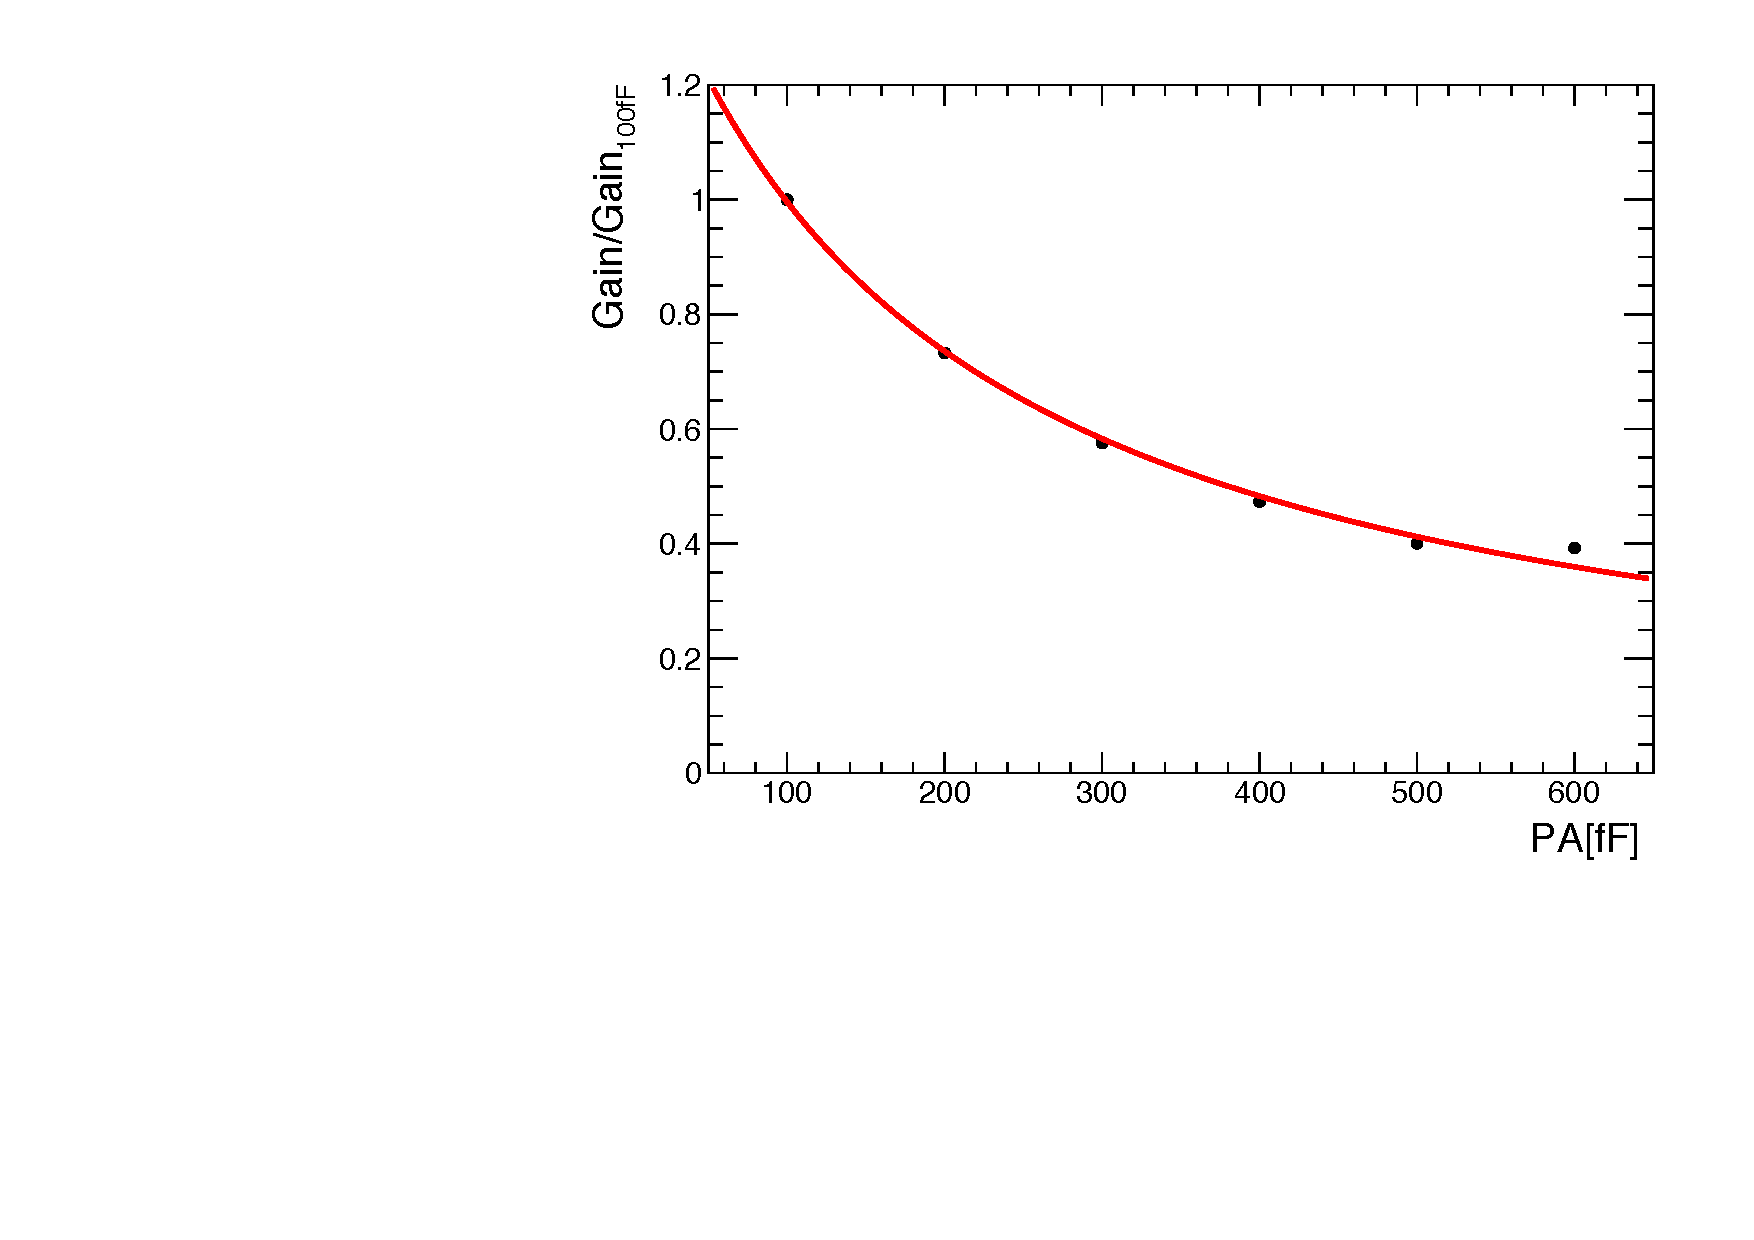
\includegraphics[width=1.\linewidth]{../Thesis_Plots/Commissioning/Plots/GainvsPA.pdf}
    \caption{} \label{fig:PA_curve}
  \end{subfigure}
  \hfill
  \begin{subfigure}[t]{0.49\textwidth}
    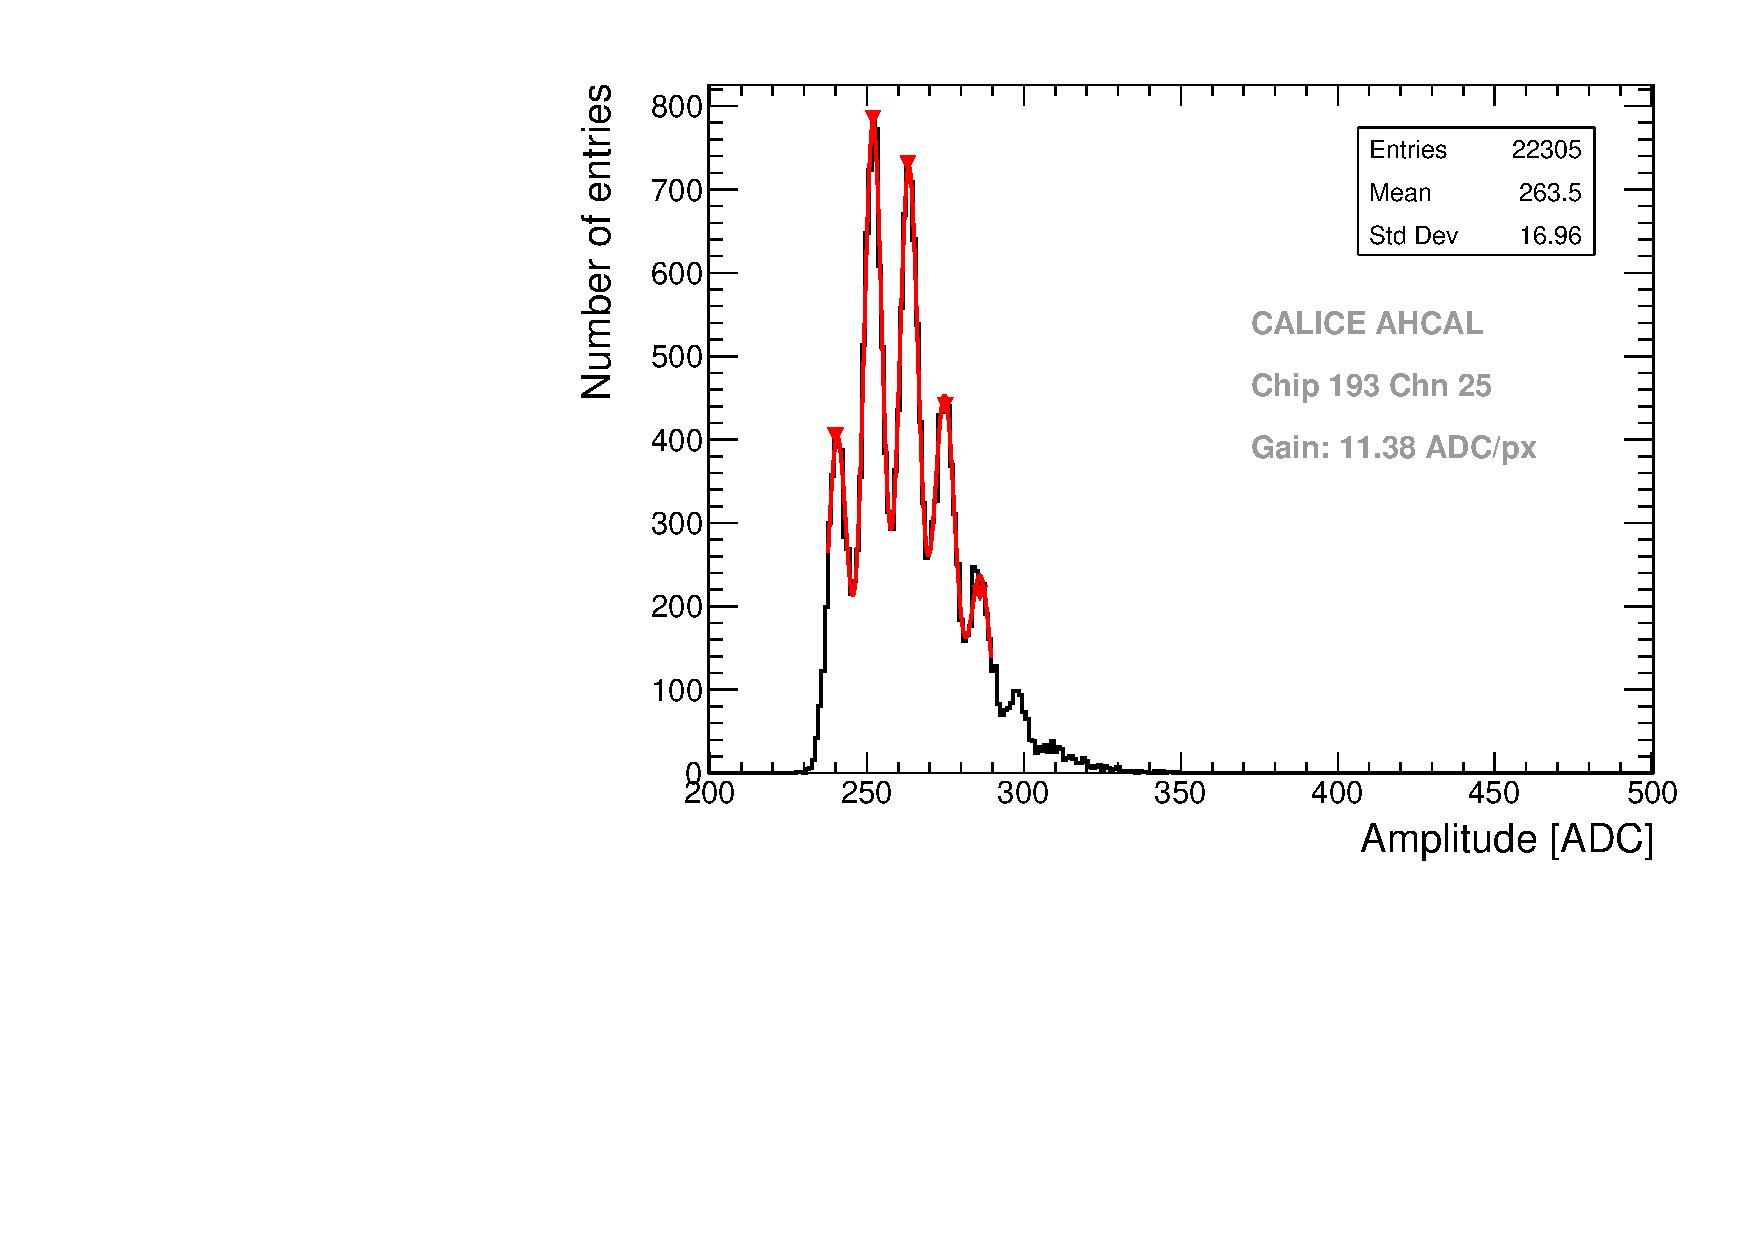
\includegraphics[width=1.\linewidth]{../Thesis_Plots/Commissioning/Plots/Gain675fF_MainzHBU4.pdf}
    \caption{} \label{fig:Gain675fF}
  \end{subfigure}
  \caption{\subref{fig:PA_curve}) Generic curve obtained with the new ITEP board used to determine the value of the pre-amplifier feedback capacitor to use. \subref{fig:Gain675fF}) Results of the gain fit for the same channel as shown above after adjustment of the pre-amplifier feedback capacitor from 100 fF to 675 fF.}
\end{figure}

\subsection{Threshold scan}

This procedure is rather new and was developed by a summer student in 2014. A better description of the procedure can been read in \cite{Hartbrich:2016bbz} and \cite{LloydTrigger}. The SPIROC2B offers the possibility of setting a global trigger threshold (10 bit range) as well as individual channel-wise threshold (4 bit range) in auto-trigger operation. The trigger threshold needs to be setup properly in order to avoid loss of information if set too high or being overwhelmed by noise events if set too low. The goal of this method is to get a good idea (to an order of 5-10\%) of the needed value for the trigger threshold in a quick and efficient way.

\begin{figure}[htbp!]
  \centering
  \begin{subfigure}[t]{0.49\textwidth}
    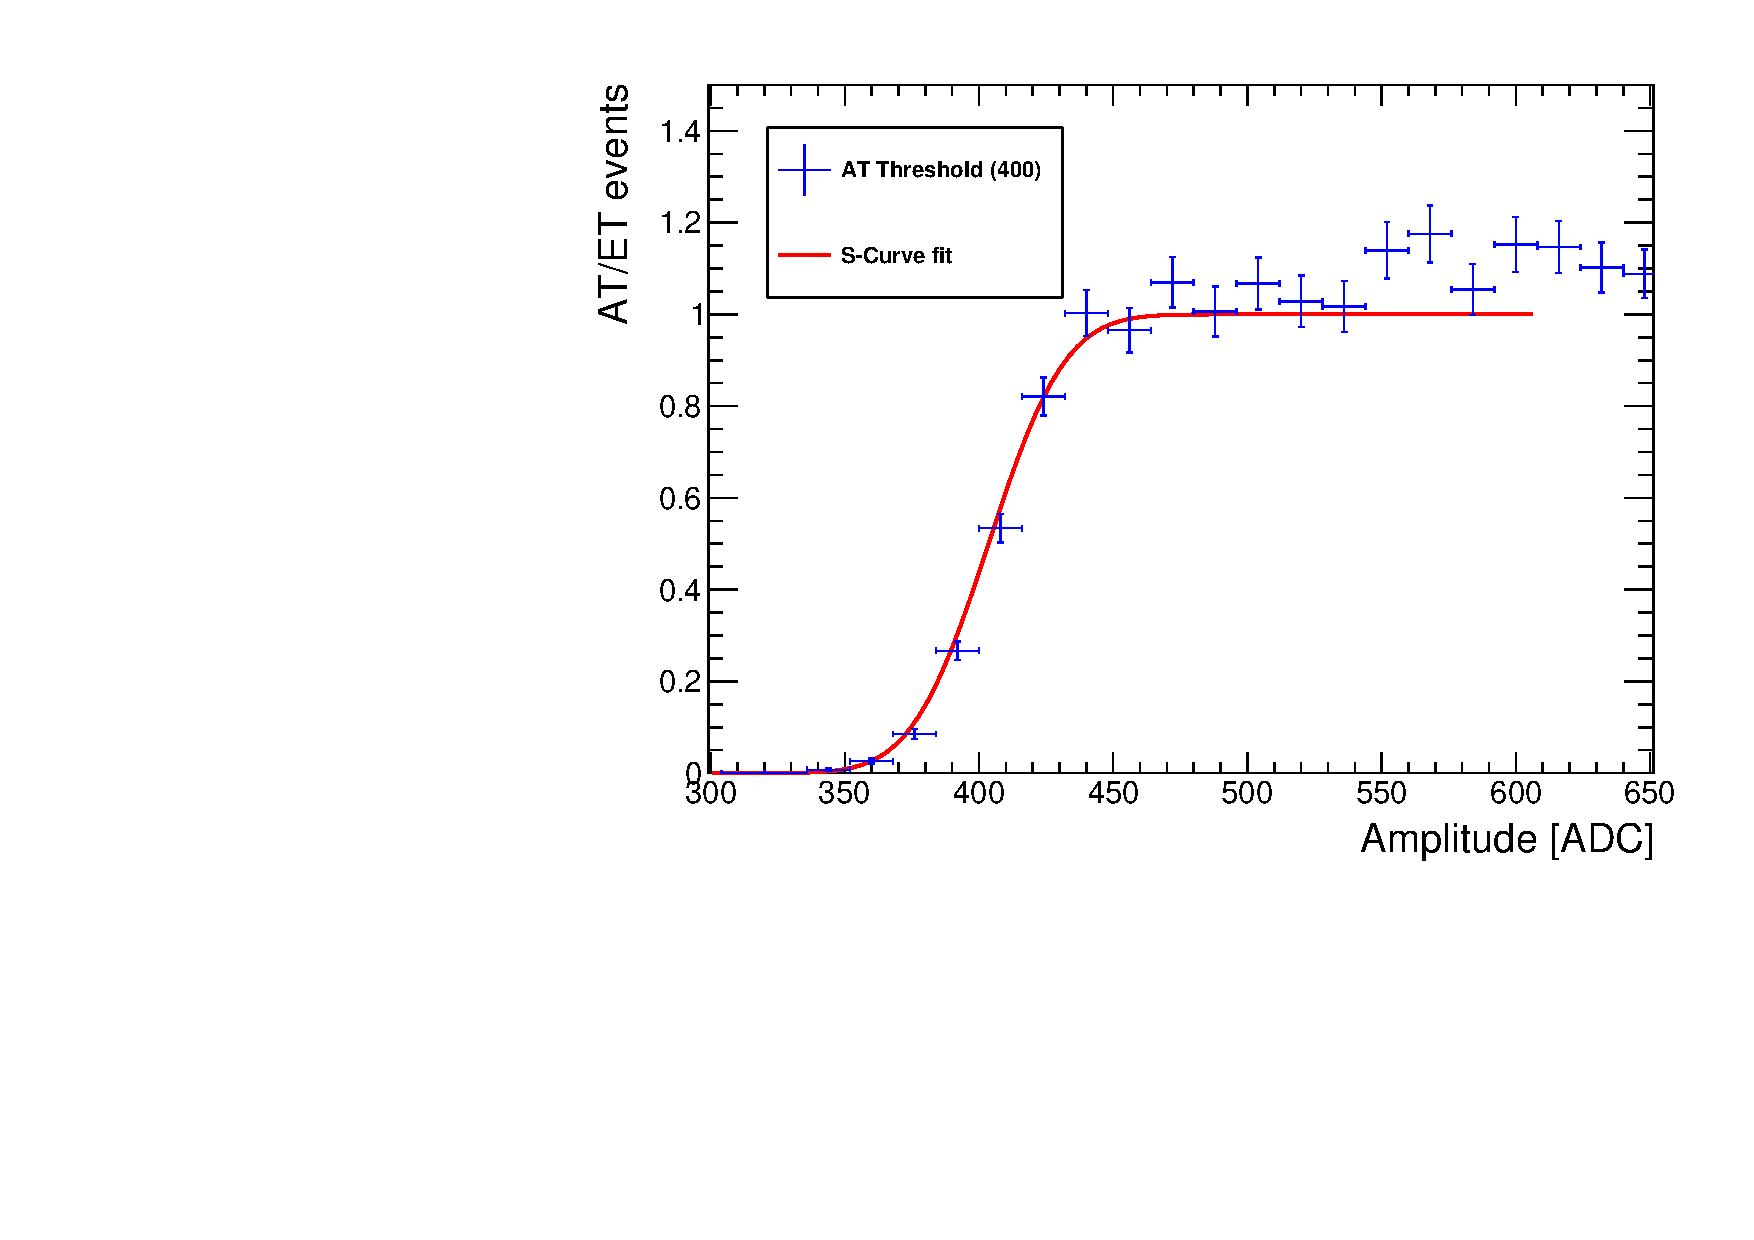
\includegraphics[width=1.\linewidth]{../Thesis_Plots/Commissioning/Plots/EfficiencyCurveFit_HBU2_12.pdf}
    \caption{} \label{fig:EffiCurve}
  \end{subfigure}
  \hfill
  \begin{subfigure}[t]{0.49\textwidth}
    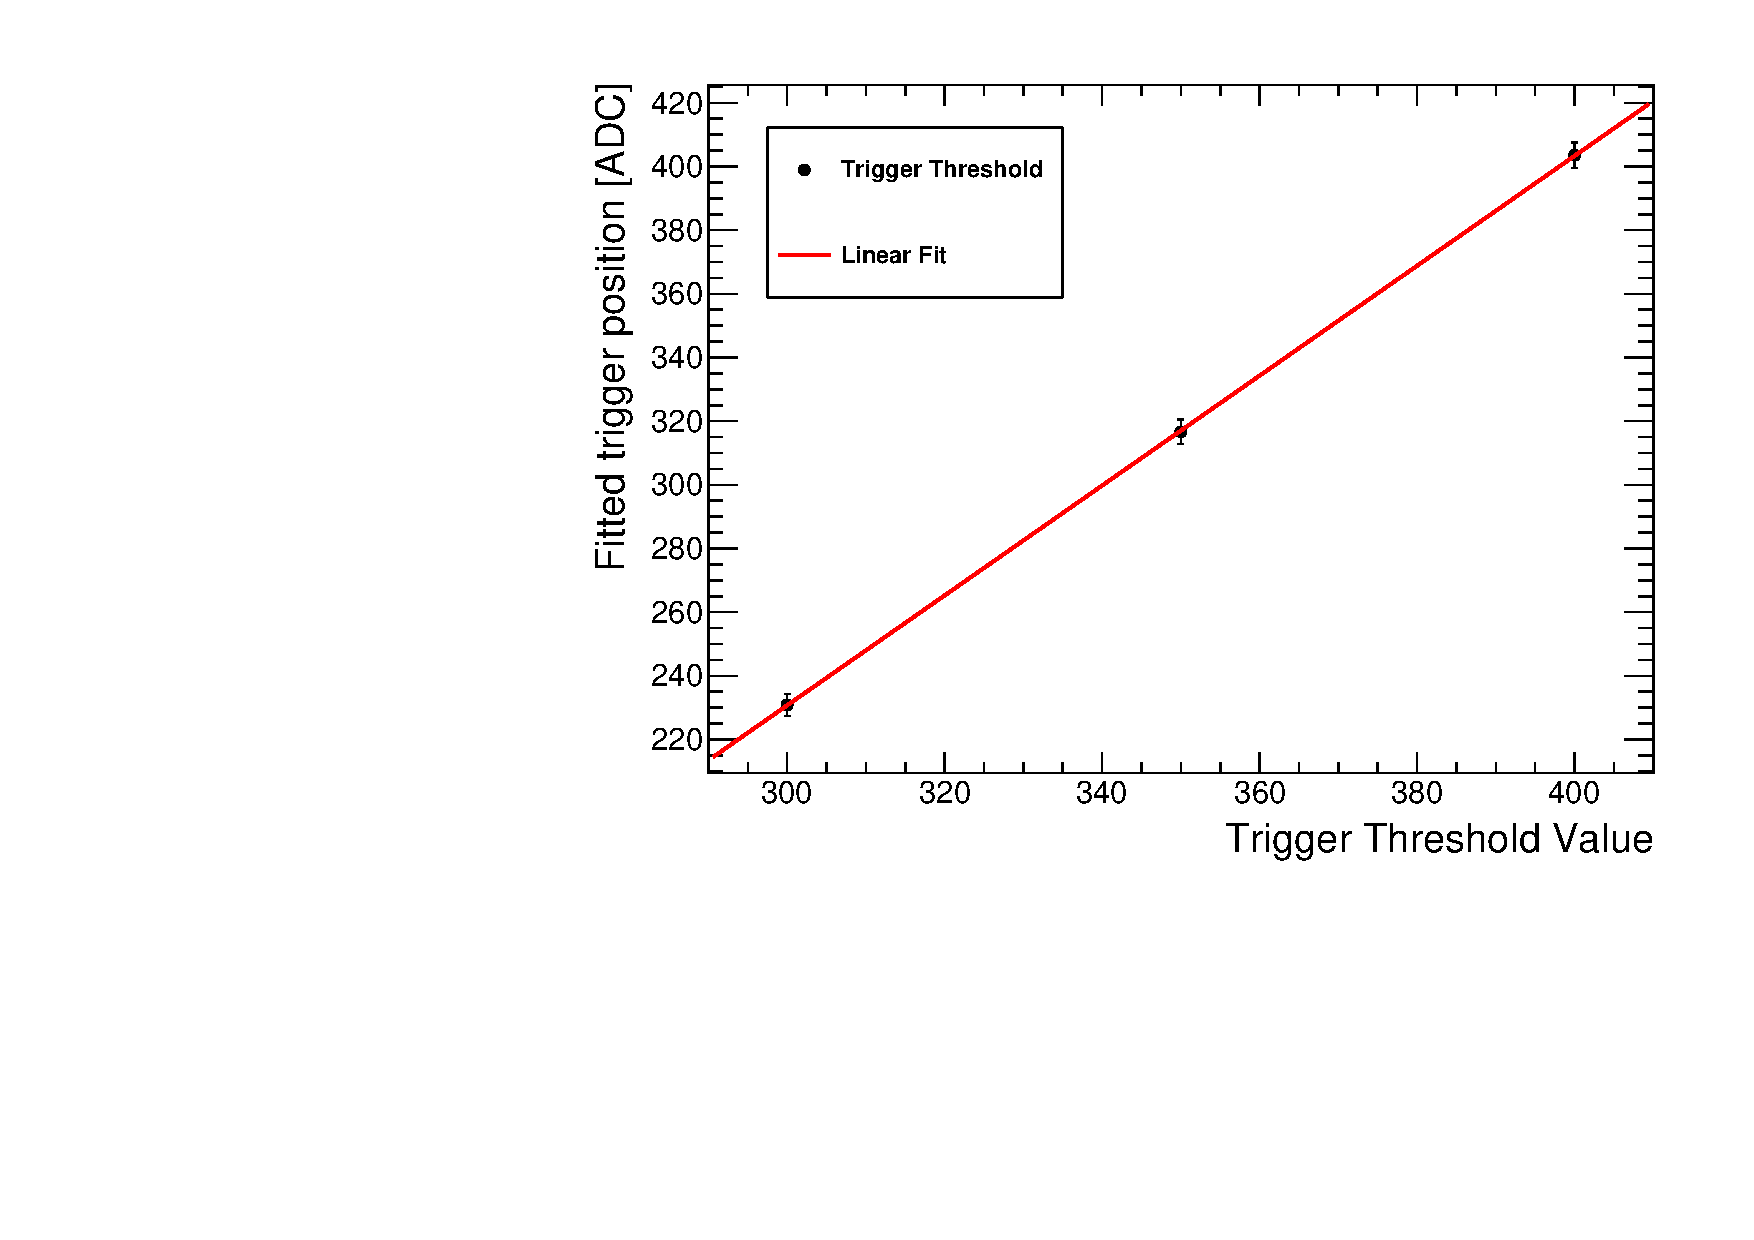
\includegraphics[width=1.\linewidth]{../Thesis_Plots/Commissioning/Plots/TriggerThresholdFit_HBU2_12.pdf}
    \caption{} \label{fig:TriggerFit}
  \end{subfigure}
  \caption{\subref{fig:EffiCurve}) Trigger efficiency S-Curve fit for a typical channel at a trigger threshold of 400. $\mu$ = 403.542 $\pm$ 4.04538. \subref{fig:TriggerFit}) Extracted trigger threshold positions as a function of the trigger threshold value. One can observe a linear behavior.}
\end{figure}

An example of the results for a single channel is shown in figure \ref{fig:EffiCurve} and \ref{fig:TriggerFit}. The efficiency is normalized to 1 due to the measurement method. The statistical uncertainty on the trigger position is around 1\% which is well below the needed accuracy. The dependence of the trigger position on the threshold parameter is linear as expected.

\section{Noise Measurement in the AHCAL}

Noise measurement is needed and complementary to the previous method. As explain above, the setting of the trigger threshold is very crucial. If the threshold is setup too low, a noisy channel could overflow the whole detector thus reducing the readout efficiency. This method is a proof-of-concept that seems to fulfill the requirement of characterizing the threshold position for all the channels or a chip at once. The needed accuracy is also here not so crucial in order to keep the threshold in the acceptable range of 0.5 MIP. This method enables us to have an idea of the noise level at a certain trigger threshold and especially to understand the evolution of noise as function of the trigger threshold. This measurement method utilizes the fact that SiPM noise should follow a Poisson distribution. Moreover to eliminate the effect of the temperature on SiPM noise, the measurement is performed in a climate chamber to a temperature of around 25 degrees Celsius.

Each measurements are taken in auto-trigger mode for different time window ($T$), from 1 ms to 30 ms, for different values of trigger threshold. Each measurement are done 200 times. Then for each run, the number of filled memory cell is filled to an histogram per chip. In a next step, each histograms are fitted with a Poisson distribution prior to the fit, it is checked that the bin 15 of the histogram is not filled otherwise the chip would be automatically readout. This is done to ensure that the measurement is stopped at exactly the end of the time window and not before. A typical example of a chip can be seen in figure \ref{fig:MemPoison}. The MPV $\lambda_{mem}$ of the Poisson distribution give us the most probable number of memory cells filled per chip for a specific trigger threshold value and time window $T$. This can then be converted into a noise rate as $DCR = \frac{\lambda_{mem}}{T}$ and filled into an histogram per chip for each trigger threshold value. Finally, the mean of this histogram is used to plot the noise rate as a function of the trigger threshold value for each chip. The figure \ref{fig:DCRThr} shows the results obtained for a typical board.

\begin{figure}[htbp!]
  \centering
  \begin{subfigure}[t]{0.49\textwidth}
    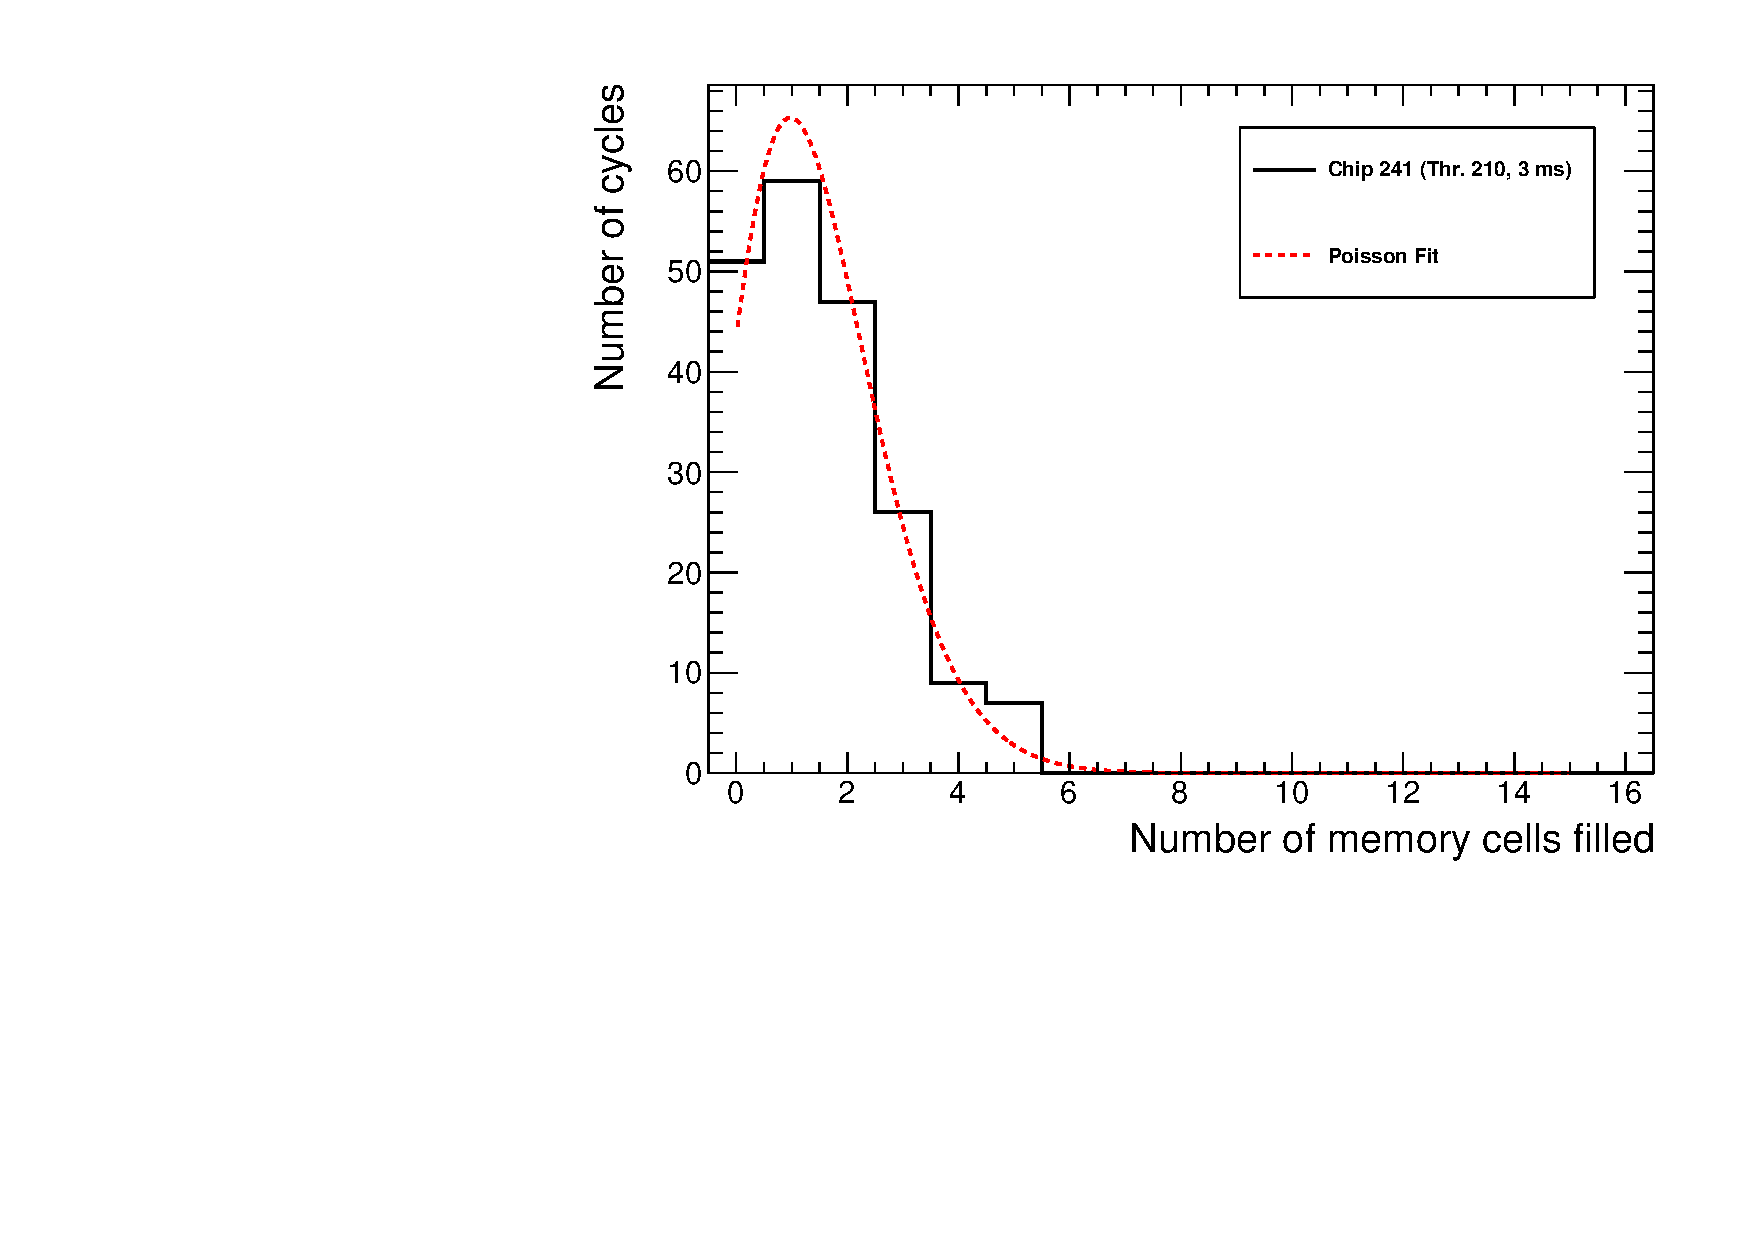
\includegraphics[width=1.\linewidth]{../Thesis_Plots/Commissioning/Plots/NumberMemFilled_Poisson.pdf}
    \caption{} \label{fig:MemPoison}
  \end{subfigure}
  \hfill
  \begin{subfigure}[t]{0.49\textwidth}
    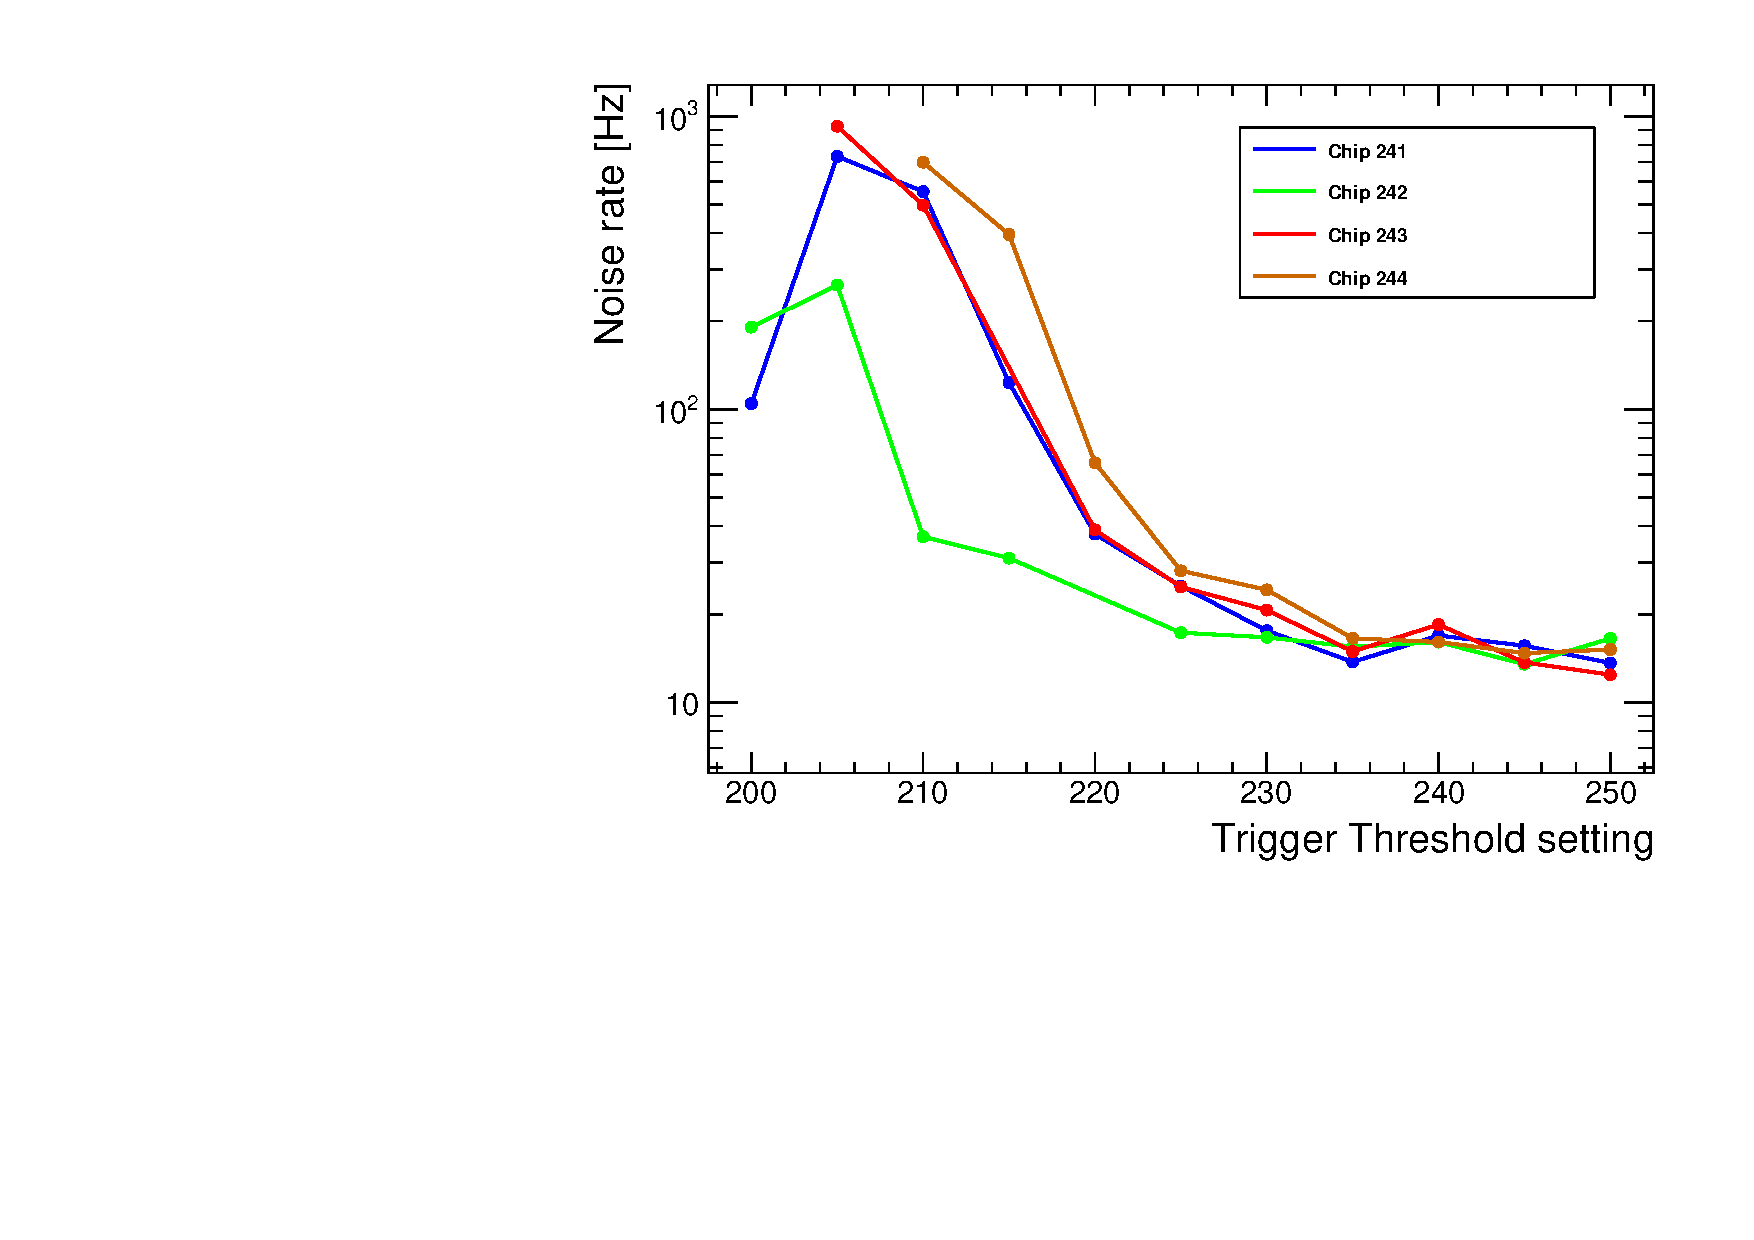
\includegraphics[width=1.\linewidth]{../Thesis_Plots/Commissioning/Plots/NoiseMeasurement_SM1.pdf}
    \caption{} \label{fig:DCRThr}
  \end{subfigure}
  \caption{\subref{fig:MemPoison}) Observed histogram of the number of memory cells filled per cycle for a typical chip with a trigger threshold of 210 and a time window $T$ of 3 ms. $\lambda_{mem}$ = 1.5 $\pm$ 0.1.\subref{fig:DCRThr}) Extracted noise rate as a function of the trigger threshold setting for a full board.}
\end{figure}

The figure \ref{fig:DCRThr} shows that noise decreases fast with increasing threshold until a plateau is reach. This plateau is the ideal area to set the threshold as noise is quite constant and does not vary a lot. In this figure, a threshold between 230 and 240 seems appropriate. As this method is complementary to the threshold scan, the region can be compared to where is the threshold put in terms of MIP value. For this board, a threshold of 230-240 corresponds to about a threshold 0.2-0.25 MIP which is well below 0.5 MIP and thus safe.

This method is very complementary to the threshold scan and can be used to set a relatively safe trigger threshold for all chips. It does not rely on a very precise measurement and has been shown to work well for all chips. Moreover this method requires only minimal additional time to the commissioning procedure. A great understanding of the position of the trigger threshold relative to 0.5 MIP would greatly improve the characterization as well as the data taking efficiency of future AHCAL engineering prototypes.


%% AHCAL Analysis
%!TEX root = ../main.tex
\part{Data Analyses}
\label{chap:TimingAHCAL}

\chapter{AHCAL Testbeam setup \& Event Selection}
\label{chap:EvtSelection}

%%% Need to rethink about this...
The experimental data used in this thesis has been collected in a testbeam campaign at the SPS facility at CERN in July 2015 with the AHCAL technological prototype described in section \ref{sec:AHCAL}.

The main topic of this thesis is the study of the \textit{time development of hadronic showers} and the study of the \textit{effects of timing cuts} in a hadronic calorimeter. The analysis is divided in several part. In the first part, the energy scale calibration of the AHCAL prototype is presented in chapter \ref{chap:ECalibAHCAL}. In the second part, the timing calibration of the AHCAL is presented in chapter \ref{chap:TimingCalib}. In a third part, the cross-check of the time calibration and the validation of the simulation is shown in chapter \ref{chap:TimingValidation}. Finally, the analysis of the recorded pion data is described in chapter \ref{chap:TimingPions}.

This chapter discusses the setup of the testbeam first before presenting the selected dataset for this analysis, the selection of the triggers needed for this analysis as time reference and the selection criteria for each dataset of muons, electrons and pions.

The key results presented in this thesis are being approved by the CALICE Collaboration and are soon to be published as \textit{CALICE Analysis Note 061: Timing of hadron showers in the CALICE Analog Hadronic Calorimeter prototype using steel absorber} (CAN-061) \cite{CAN061}. The analysis in this thesis is the first of its kind to such a system level and enters new territories for high granular calorimeters.

\section{Testbeam Configuration}

\subsection{Beamline Setup}
\label{sec:beamline}

During the summer of 2015, the CALICE collaboration performed several testbeam campaigns with the AHCAL technological prototype. The detector was installed in the beamline H2 in the SPS North Area at CERN \cite{H2Beamline}. This beamline is equipped with wire chambers and scintillators that provide information of the beam position and number of particles. The wire chamber information would have been useful in order to simulate correctly the beam profile. Unfortunately, this information could not be recorded with the AHCAL data acquisition system. The information available about the amount of material upstream of the detector until the last momentum selection magnet is limited thus the simulation of the beamline is simplified.

A Cherenkov detector (at around 100 m upstream) was available to tag incoming particles. These detectors take advantage of the fact that, a particle that traverses a medium faster than the speed of light in that medium will generate a cone of Cherenkov light. The opening angle of the cone is proportional to the particle mass \cite{GOVORKOV20059}. The Cherenkov detector at this beamline offered the possibility to set a threshold for particle tagging. This is particularly needed to tag possible contaminating electrons in a pion beam. The tagging signal from the Cherenkov detector was provided directly to several AHCAL channels.

For the production of particles, a primary high-intensity proton beam (around $10^{12}$ protons per burst) of 400 GeV impinges on a target. From this, a secondary beam is produced containing various particle types and energies.

A muon beam can be obtained from the decay of a collimated pion beam which are stopped by a collimator before the last bending magnet.

For electrons, a neutral beam of photons is directed to a lead target to generate electrons from gamma conversion, producing a very pure electron beam. Another possibility is to impinge a charged beam onto a secondary target and filter the beam with an absorber. But this has the disadvantage of low rates at low energy and possible contamination of the electron beam with pions \cite{H2Beamline}.

For pions, the momentum is selected via a set of collimators and magnets. Due to the decay of $\pi_0$ (conversion of the photons into the absorber filter) and the acceptance of the beamline, a contamination of the pion beam with electrons is possible at low momentum (< 20 GeV).

\subsection{Testbeam Setup}
\label{sec:TBsetup}

In July 2015, the AHCAL detector was using the full EUDET steel stack \cite{EUDET-Report-2010-02} with 48 iron absorber plates. In the stack, 14 active modules were installed. The two first layers consist of single ECAL Base Units (EBUs) with $4 * 36$ cells of $4.5 * 0.5$ cm$^2$ size (ECAL). The ECAL cells of both layers are oriented parallel to the x-axis. The next eight layers consist of single HCAL Base Units (HBUs) with $12 * 12$ cells of $3 * 3$ cm$^2$ size (HCAL). The first 10 layers correspond to a depth of around 10 X$_0$ ($\sim$ 1 $\lambda_{\pi}$). These layers mainly used as a shower start finder. The last four layers consist of 2 by 2 HBUs providing information about the development of pion showers at different depths. The detector was placed on a movable stage in order to be able to move the detector position relative to the beam for muon calibration runs. A simplified view of the beamline configuration is shown in figure \ref{fig:TestbeamScketch}.

\begin{figure}[htbp!]
	\centering
	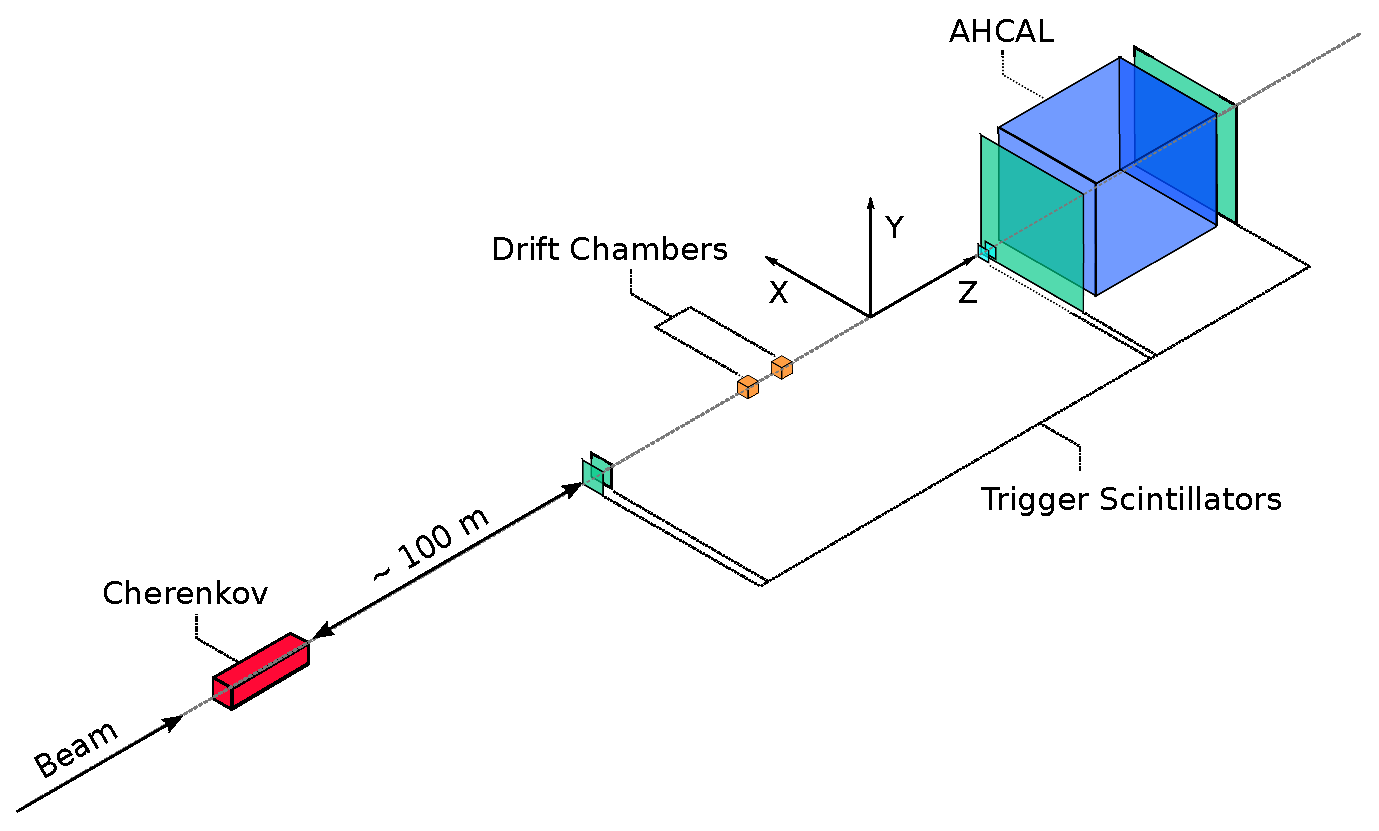
\includegraphics[width=0.7\linewidth]{chap5/fig_EnergyCalib/TestbeamSetup.eps}
	\caption{Sketch view of the beamline setup at the CERN SPS H2 beamline in July 2015.} \label{fig:TestbeamScketch}
\end{figure}

\begin{figure}[htbp!]
	\centering
	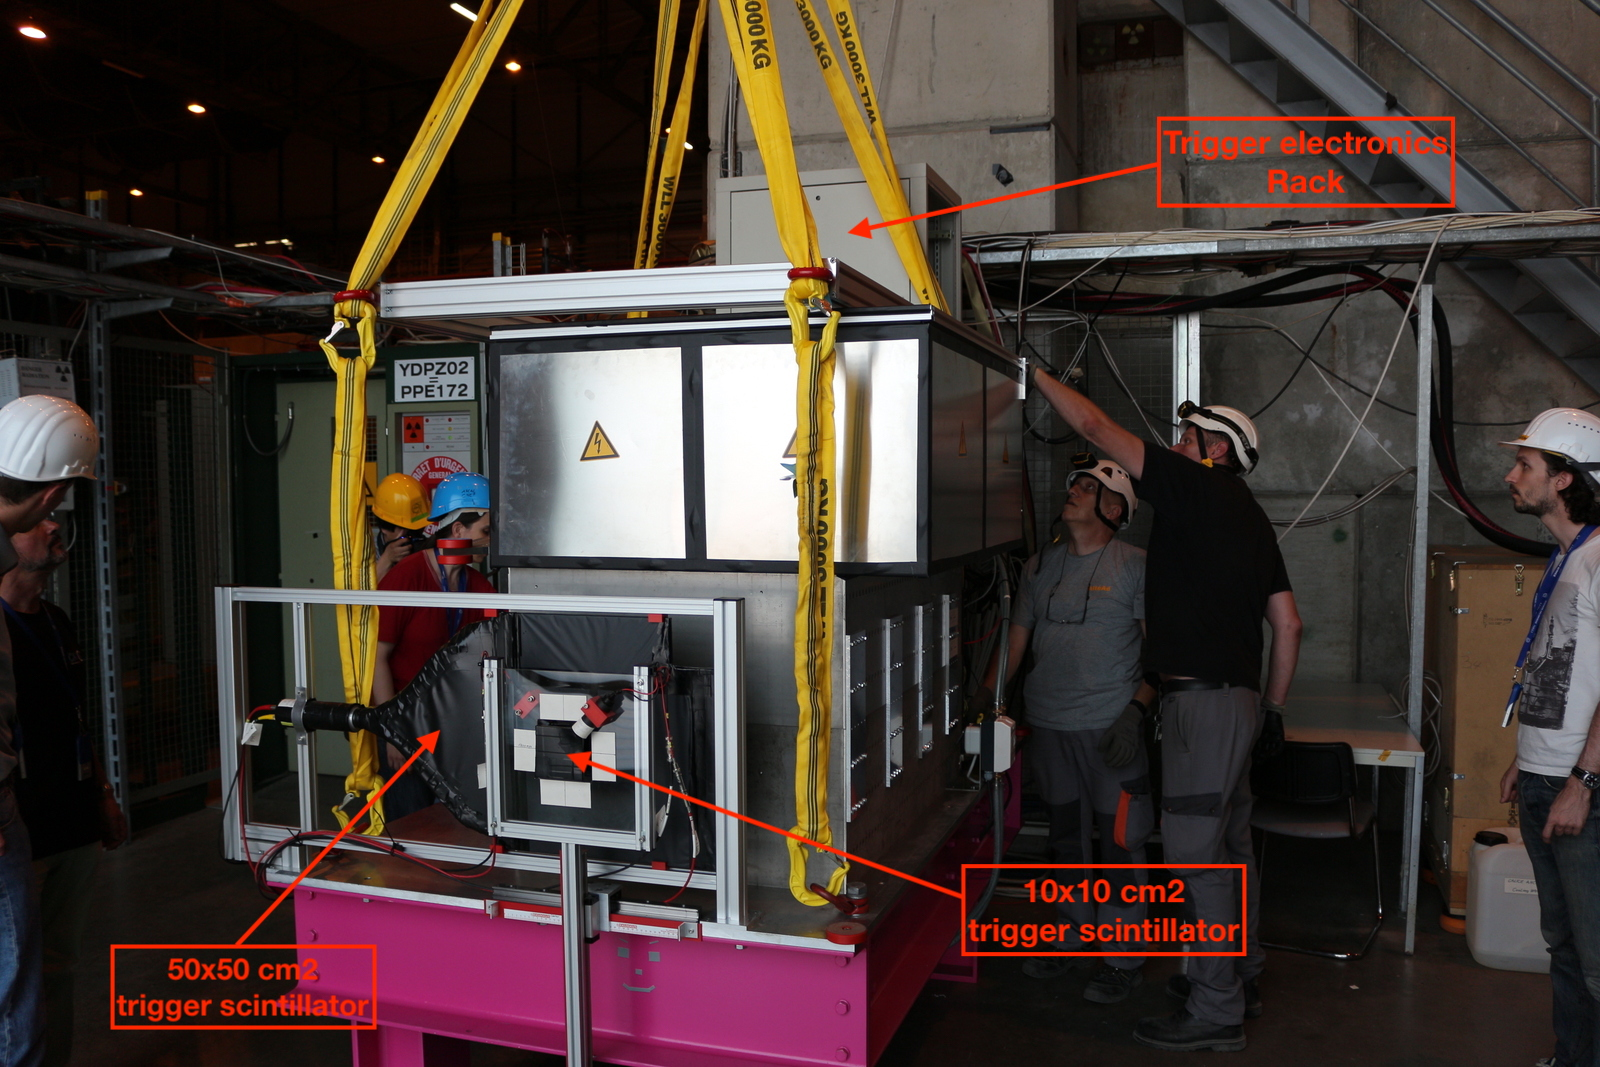
\includegraphics[width=0.7\linewidth]{chap5/fig_EnergyCalib/IMG_1170_copy.jpg}
	\caption{Photo of the AHCAL detector during the installation in the testbeam area.} \label{fig:AHCAL_photo}
\end{figure}

The beam instrumentation consisted of two $10\times10$ cm$^2$ scintillator plates in front of the calorimeter, and two $50\times50$ cm$^2$ scintillator plates, one placed in front of the calorimeter and one placed at the back of the calorimeter as shown in figure \ref{fig:AHCAL_photo}. They are read-out by photomultiplier tubes. The coincidence of the $50\times50$ cm$^2$ scintillator plates was used for the muon runs and the coincidence of the $10\times10$ cm$^2$ scintillator plates is used for the electron and pion runs as a trigger signal.

Additionally, the coincidence signal from the scintillator was provided directly to several channels of the AHCAL in order to provide a reference time information of the trigger which is important for the timing study presented in this thesis. A simplified view of the layer structure of the AHCAL is shown in figure \ref{fig:Det_layout}.

\begin{figure}[htbp!]
	\centering
	\includegraphics[width=0.7\linewidth]{chap5/fig_EnergyCalib/Detector_layout_copy.png}
	\caption{Simplified view of the detector layout used in July 2015.} \label{fig:Det_layout}
\end{figure}

\subsection{Time reference}
\label{subsec:trigger}

The scintillator plates were used as a time reference signal. Both type of scintillator are connected to a discriminator and a gate for coincidence in order to provide a validation signal to the readout chip (see section \ref{sec:SPIROC2B}).

When a coincidence happens, a signal of 4 $\mu$s length with a fast rising edge of around 1 ns, is generated with an amplitude around 100 mV that is used as a time reference. This signal is provided \textit{directly to six AHCAL channels} for redundancy. The list of the AHCAL channels used as a reference time are shown in table \ref{table:trigger_signal_list}. No other external time reference was available.

\begin{table}[htb!]
	\centering
	\caption{List of AHCAL channels used as time reference for this analysis.}
	\label{table:trigger_signal_list}
	\begin{tabular}{@{} ccccc @{}}
		\toprule
		Layer \# & Chip Number & Channel & Comments & Name \\
		\midrule
		11 & 169 & 29 & noisy & T$_{11}$ \\
		11 & 177 & 23 & broken & - \\
		12 & 185 & 29 & - & T$_{12}$ \\
		13 & 201 & 29 & -  & T$_{13}$ \\
		13 & 211 & 6 & broken & - \\
		14 & 217 & 23 & - & T$_{14}$ \\
		\bottomrule
	\end{tabular}
\end{table}

In the following analysis, the time reference signals T$_{12}$, T$_{13}$ and T$_{14}$ are used. The channels are determined to be noisy or broken by looking at the energy spectra of these channels. Broken channels results in an empty energy spectrum and noisy channels are showing two energy peaks, one near the pedestal and another at the expected energy value. The channel T$_{11}$ is not used as it presented a very low efficiency due to noise.

\section{Dataset and Event Selection}

The selections presented in this section are based on simulated data. Beforehand, the simulation has been carefully validated and represents within 10-20\% the data in muon and electron beam. More details can be seen in section \ref{sec:SimulationVal}.

\subsection{Dataset}
\label{subsec:dataset}

During the campaign at the CERN \acrshort{sps} facility in July 2015, firstly, muon runs were taken at beam energies of 50 GeV and 150 GeV for calibrating the detector. Secondly, several electron runs were taken at beam energies between 10 GeV and 50 GeV to study the electromagnetic response of the calorimeter. Finally, the pion runs were taken at beam energies between 10 GeV and 90 GeV.

The table \ref{table:dataruns} sums up the datasets taken in different beams. The number of events shown in the table is the total number of recorded events.

\begin{table}[htb!]
	\centering
	\caption{List of runs taken at SPS in July 2015.}
	\label{table:dataruns}
	\begin{tabular}{@{}lp{2cm}p{7.5cm}p{2cm}@{}}
		\toprule
		\multicolumn{1}{l}{\textbf{Particle}} & \textbf{Energy} & \textbf{Runs} & \textbf{\# Events}\\
		\midrule
		\multirow{2}{*}{$\mu^-$}& 50 GeV & 24016-24204 & 120,887,651\\& 150 GeV & 24623-24662 & 15,534,328\\
		\midrule
		\multirow{2}{*}{e$^-$}& 10 GeV & 24531-24576 & 38,028,438\\& 15 GeV & 24507-24527 & 7,701,325\\& 20 GeV & 24479-24504 & 10,498,554\\& 30 GeV & 24454-24475 & 3,382,943\\& 40 GeV & 24420-24448 & 2,665,843\\& 50 GeV & 24404-24419 & 5,933,995\\
		\midrule
		\multirow{2}{*}{$\pi^-$}& 10 GeV & 24266-24272, 24300-24317, 24381-24397 & 24,311,420\\& 20 GeV & 24398-24400 & N/A\footnotemark\\& 30 GeV & 24259-24299, 24319-24380 & 10,120,753\\& 50 GeV & 24212-24254, 24325-24357, 24580-24612 & 10,704,661\\& 70 GeV & 24219-24242, 24365-24374 & 8,885,407\\& 90 GeV & 24233-24287, 24331-24364 & 7,955,604\\
		\bottomrule
	\end{tabular}
\end{table}

\subsection{Muon selection}
\label{subsec:Muon_presel}

\subsubsection{Pre-selection}

A clean selection of MIP-like particles is needed in order to obtain and cross-check the energy scale calibration of the AHCAL (see chapter \ref{chap:ECalibAHCAL}) and as well performing the timing calibration of the detector (see chapter \ref{chap:TimingCalib}) at a single cell level. A simple pre-selection was performed on the muon dataset designed to select MIP-like particles going through the AHCAL. In a second step, a track selection was performed to retain only MIP-like particle as explained in section \ref{subsec:Muon_sel}.

The pre-selection is based on the energy weighted center of gravity along the beam axis $cog_Z = \frac{\Sigma{i} E_i z_i}{\Sigma_{i} E_i}$ and the number of hits $n_{Hits}$. A MIP-like particle should, in principle, deposit the same energy in each layer of the calorimeter thus $cog_Z$ should be roughly centered in the calorimeter in the z coordinate. In addition, the number of hits should be around 1 per layer for a MIP-like particle plus the number of noise hits expected in the detector, therefore explaining a cut at $n_{Hits} = 20$.

The distribution in the plane $cog_Z$:$n_{Hits}$ shown in figure \ref{fig:Muons_CoGZ_nHits} is obtained from simulated 150 GeV muons, electrons and pions. The applied pre-selection is represented by the black box. The pre-selection removes few muon events, as well as it discards electrons greatly and rejects also a large fraction of pions. The pre-selection efficiency is 99.4\% for muons, 0\% for electrons and 13.3\% for pions.

\begin{figure}[htbp!]
	\centering
	\includegraphics[width=0.7\linewidth]{../Thesis_Plots/Timing/Muons/Plots/SelectionCut_nHitsCoGZ_Muons.eps}
	\caption{Event distribution in $cog_Z:n_{Hits}$ plane. The size of each box represents the number of events in each bin. The black box represents the space-phase covered by the pre-selection.} \label{fig:Muons_CoGZ_nHits}
\end{figure}
\footnotetext{Not analyzed due to limited dataset.}

\subsubsection{Selection}
\label{subsec:Muon_sel}

By looking at the spectrum of the number of hits per event, it is estimated that around 30\% of the events in the muon runs are contaminated by pions.

The MIP selection was designed to efficiently select muons and reject late pion showers. For this, a MIP track finder has been developed based on previous work \cite{Hartbrich:2016bbz}. This algorithm is designed to select MIP-like particle tracks in the AHCAL detector and remove pion showers.

The algorithm selects AHCAL towers of hits in the same $x:y$ position and it rejects AHCAL towers that contains less than a certain number of hits. In order to select muons or punch-through pions, a straight track of at least 7 hits is required in the whole AHCAL. This assumes that the calorimeter was perfectly perpendicular to the beam, therefore any tilted tracks would be missed. In addition, to reject late pion showers, no more than 2 hits are allowed per layer to account for some flexibility with noise hits.

The distributions of the maximum number of hits in a layer and the number of hits of a track are shown in figures \ref{fig:Muons_Track_nHitsLayer} and \ref{fig:Muons_Track_nHits} for simulated samples of 150 GeV muons, electrons and pions after pre-selection. The MIP track finder was performed in two steps for the inner part of the detector of $12 \times 12$ tiles and the outer part for the big layers (layers 11 to 14, Outer BL) in order to calibrate the outer channels of these layers. The figure \ref{fig:Muons_Track_nHitsLayer} shows that a cut of two hits per layer is optimal in order to reject pions without affecting muons too much.

The selection efficiency is 72.5\% for muons, 0\% for electrons and 5.6\% for pions. The selection reduces further the pion contamination and the remaining pion fraction is compatible with the fraction of pions traversing the AHCAL without hard interaction. An overview of the MIP selection cuts is given in table \ref{table:muon_sel}.

\begin{figure}[htbp!]
	\begin{subfigure}[t]{0.49\textwidth}
		\centering
		\includegraphics[width=1\linewidth]{../Thesis_Plots/Timing/Muons/Plots/TrackFinderCut_nHitsLayer_Muons.eps}
		\caption{} \label{fig:Muons_Track_nHitsLayer}
	\end{subfigure}
	\hfill
	\begin{subfigure}[t]{0.49\textwidth}
		\centering
		\includegraphics[width=1\linewidth]{../Thesis_Plots/Timing/Muons/Plots/TrackFinderCut_nHitsTrack_Muons.eps}
		\caption{} \label{fig:Muons_Track_nHits}
	\end{subfigure}
	\caption{\subref{fig:Muons_Track_nHitsLayer}) Distribution of number of hits in a layer normalized to the number of events for simulated muons at 150 GeV, electrons and pions at 50 GeV. The black line represents the cut of the maximum allowed number of hits in a layer applied for the MIP selection. \subref{fig:Muons_Track_nHits}) Distribution of the number of hits in a track normalized to the number of events for simulated muons at 150 GeV, electrons and pions at 50 GeV. A AHCAL tower size cut of 7 hits for the inner 12 $\times$ 12 tiles and a AHCAL tower size of 2 hits for the layers 11 to 14 on the outer tiles (Outer BL) were chosen.}
\end{figure}

\subsection{Electron Selection}
\label{subsec:elec_sel}

The electron selection is done to extract single electron showers contained in the AHCAL. These events are needed to validate the timing behavior in simulation as well as the detector simulation model as explained in chapter \ref{chap:TimingValidation}. It is important to have a clean sample of electrons to cross-check the timing calibration. For the selection, an \textit{Event Quality} pre-selection is done using the beam instrumentation and layer information. Events with a Cherenkov tag (only applied to data) are used. The distributions of the energy deposit in the first three AHCAL layers ($E_3+E_4+E_5$) are shown in figures \ref{fig:e10GeV_E3} and \ref{fig:e50GeV_E3} for simulated muon, electron and pion beams. In order to suppress muons and pions, $E_3+E_4+E_5$ must be over 10 MIPs.

In a next step, the electron selection is performed. Usually, one could use a shower start algorithm to select electrons that interact in the first layers of the calorimeter and reject pions efficiently \cite{Hartbrich:2016bbz}. However, the first ECAL layers (see section \ref{subsec:ScECAL}) can't be used because of high noise and the detector is partially equipped with active layers. This would greatly influence the performance of such algorithm, therefore, an alternative selection is needed.

A cut on the number of hits per event ($n_{Hits}$) versus the center of gravity in z ($CoG_Z$) is done. It is shown in figures \ref{fig:e10GeV_nHitsCoGZ} and \ref{fig:e50GeV_nHitsCoGZ}. The box cut in the figures does not induce any bias for the timing study in this thesis, it would only reduce the event statistics. In addition, the number of hits in a electron shower is proportional to the shower energy, thus this cut is energy dependent.

Finally, a cut on the energy deposited in the last two layers relative to the energy deposited in the calorimeter ($(E_{13}+E_{14})/\Sigma E$) is done. The distributions are shown in figures \ref{fig:e10GeV_Elast} and \ref{fig:e50GeV_Elast}. This cut is required to be under 1\% to reject pion showers and to contain the electron shower.

Additionally, to reduce transverse leakage, the shower center of gravity in X and Y needs to be within -90 mm and 90 mm. This cut is wider than the trigger scintillator but has no significant impact. The selection efficiencies for muon, electron and pion beams are shown in table \ref{table:eff_electron} for different beam energies from 10 GeV to 50 GeV. The detailed selection cuts are summarized in appendix table \ref{table:electron_sel}.

\begin{table}[htb!]
	\centering
	\caption{Efficiency of the electron selection for simulated electrons, muons and pions for energies between 10 and 50 GeV. The efficiency is defined as the number of events after selection over the number of event before selection.}
	\label{table:eff_electron}
	\begin{tabular}{@{} llll @{}}
		\toprule
		\textbf{Beam Energy} & \textbf{$\epsilon_{\mu}$} & \textbf{$\epsilon_{e}$} & \textbf{$\epsilon_{\pi}$}\\
		\midrule
		10 GeV & <0.1\% & 96\% & 15.9\%\\
		15 GeV & <0.1\% & 95.7\% & 10.1\%\\
		20 GeV & <0.1\% & 95.2\% & 6.3\%\\
		30 GeV & <0.1\% & 93.9\% & 2.3\%\\
		40 GeV & <0.1\% & 92.7\% & 1.2\%\\
		50 GeV & <0.1\% & 91.5\% & 1.1\%\\
		\bottomrule
	\end{tabular}
\end{table}

One can notice from table \ref{table:eff_electron} that a significant fraction of pions is present at low beam energies (10 to 20 GeV). But as the production of electrons in the beamline was done using a beam of photons on a beryllium target, it is with confidence that there is no pion contamination in the data \cite{AmbraEnergy}. Thus no additional cut is needed.

\begin{figure}[htbp!]
	\begin{subfigure}[t]{0.49\textwidth}
		\centering
		\includegraphics[width=1\linewidth]{../Thesis_Plots/Timing/Electrons/Plots/SelectionCut_EnergyE3_10GeV.eps}
		\caption{10 GeV.} \label{fig:e10GeV_E3}
	\end{subfigure}
	\hfill
	\begin{subfigure}[t]{0.49\textwidth}
		\centering
		\includegraphics[width=1\linewidth]{../Thesis_Plots/Timing/Electrons/Plots/SelectionCut_EnergyE3_50GeV.eps}
		\caption{50 GeV.} \label{fig:e50GeV_E3}
	\end{subfigure}
	\hfill
	\begin{subfigure}[t]{0.5\textwidth}
		\centering
		\includegraphics[width=1\linewidth]{../Thesis_Plots/Timing/Electrons/Plots/SelectionCut_nHitsCoGZ_10GeV.eps}
		\caption{10 GeV.} \label{fig:e10GeV_nHitsCoGZ}
	\end{subfigure}
	\hfill
	\begin{subfigure}[t]{0.5\textwidth}
		\centering
		\includegraphics[width=1\linewidth]{../Thesis_Plots/Timing/Electrons/Plots/SelectionCut_nHitsCoGZ_50GeV.eps}
		\caption{50 GeV.} \label{fig:e50GeV_nHitsCoGZ}
	\end{subfigure}
	\hfill
	\begin{subfigure}[t]{0.5\textwidth}
		\centering
		\includegraphics[width=1\linewidth]{../Thesis_Plots/Timing/Electrons/Plots/SelectionCut_EnergyLastLayers_10GeV.eps}
		\caption{10 GeV.} \label{fig:e10GeV_Elast}
	\end{subfigure}
	\hfill
	\begin{subfigure}[t]{0.5\textwidth}
		\centering
		\includegraphics[width=1\linewidth]{../Thesis_Plots/Timing/Electrons/Plots/SelectionCut_EnergyLastLayers_50GeV.eps}
		\caption{50 GeV.} \label{fig:e50GeV_Elast}
	\end{subfigure}
	\caption{Distribution of the variables used in the electron selection of simulated electron and pion beams between 10 and 50 GeV. The muons are simulated at 150 GeV. These plots were used to determine the best selection criteria for electrons.} \label{fig:electronselection}
\end{figure}

\subsection{Pion Selection}
\label{sec:pionsel}

The goal of the pion selection is to reject punch-through pions, muons and possible electron contamination as these events would be instantaneous (see section \ref{sec:TimeDevShowers}). An \textit{Event Quality} pre-selection is performed using the Cherenkov information. The events without a Cherenkov tag are selected. This is only applied to data. The pion selection is based on the same variables as the electron selection: $cog_Z:n_{Hits}$ plane, $(E_{13}+E_{14})/\Sigma E$ and additionally the number of hits in two first AHCAL layers ($N_3+N_4$).

Firstly, the distribution of events in the $cog_Z:n_{Hits}$ plane is shown in figures \ref{fig:pi10GeV_nHitsCoGZ} and \ref{fig:pi90GeV_nHitsCoGZ} for muon, electron and pion beam energies from 10 GeV to 90 GeV. The number of hits required per event needs to be over 20 to reject most muons or punch-through pions without cutting on the center of gravity in z in order not to bias the start of the pion shower.

Secondly, the distributions of the energy fraction deposited in the two last AHCAL layers are shown in figures \ref{fig:pi10GeV_Elast} and \ref{fig:pi90GeV_Elast}. This variable must be over 1\% in order to ensure that pion showered and reject electrons. Finally, the distributions of the number of hits in the two first AHCAL layers is shown in figure \ref{fig:pi10GeV_N3N4} and \ref{fig:pi90GeV_N3N4}. The number of hits in the two first AHCAL layers must be under 5 to mitigate possible particle contamination from electrons.

The selection efficiencies for muon, electron and pions beams for different beam energies between 10 and 90 GeV are shown in table \ref{table:eff_pion}. At 10 GeV, one can observe a low pion selection efficiency that is due to the fact less energy is deposited in the last two layers of the AHCAL thus reducing the number of selected pion events.

\begin{table}[htb!]
	\centering
	\caption{Efficiency of the pion selection for beam energies between 10 and 90 GeV. The efficiency is defined as the number of events after selection over the number of event before selection.}
	\label{table:eff_pion}
	\begin{tabular}{@{} llll @{}}
		\toprule
		\textbf{Beam Energy} & \textbf{$\epsilon_{\mu}$} & \textbf{$\epsilon_{e}$} & \textbf{$\epsilon_{\pi}$}\\
		\midrule
		10 GeV & <0.1\% & <0.1\% & 29.9\%\\
		30 GeV & 0.9\% & <0.1\% & 50.3\%\\
		50 GeV & 0.9\% & <0.1\% & 51.1\%\\
		70 GeV & 0.9\% & <0.1\% & 51\%\\
		90 GeV & 0.9\% & <0.1\% & 50.2\%\\
		\bottomrule
	\end{tabular}
\end{table}

In addition, multiple particle events were observed in the data as shown in figure \ref{fig:DoubleParticleEvent}. As no beam instrumentation could be used for rejecting these events, a rejection method based on the hit time information was developed.

\begin{figure}[htbp!]
	\centering
	\includegraphics[width=0.7\linewidth]{chap5/fig_AHCAL_timing/Pions/DoubleParticleEventPions.png}
	\caption{Multi-particle event in the 50 GeV pion data sample. The colors represent the time of the hit: green < 5 ns, blue 5 ns to 15 ns, yellow 15 ns to 35, orange 35 ns to 50 ns and red > 50 ns. One can observe an additional late muon going through the detector.} \label{fig:DoubleParticleEvent}
\end{figure}

The method is the following: all the hits in an event are placed and ordered in time; Then for each hit after 50 ns, a timing window of 30 ns used. The number of hits in that window are counted. If the number of hits is larger than 5, it is classified as a \textit{late cluster}. The event is rejected if there is at least one late cluster. This method works because if an event has several particles, the time reference of the event is generated by the first particle. Therefore, the second particle will have all the hits late relative to the time reference and thus the event will be rejected.

The method is based on data in order to remove multi-particle events. The multi-particle event rejection has been checked on simulated data and affects the selection between <0.1\% up to 2\% from 10 to 90 GeV pions. These multi-particle events are greatly suppressed in data. The number of events removed varies between 0.1\% and 1\% depending on the beam energy. Due to the calorimeter not being fully equipped thus providing limited information, some contamination may remain in the data.

A detailed description of the selection cuts are shown in appendix table \ref{table:pion_sel}.

\begin{figure}[htbp!]
	\begin{subfigure}[t]{0.49\textwidth}
		\centering
		\includegraphics[width=1\linewidth]{../Thesis_Plots/Timing/Pions/Plots/SelectionCut_N3N4_10GeV.eps}
		\caption{10 GeV.} \label{fig:pi10GeV_N3N4}
	\end{subfigure}
	\hfill
	\begin{subfigure}[t]{0.49\textwidth}
		\centering
		\includegraphics[width=1\linewidth]{../Thesis_Plots/Timing/Pions/Plots/SelectionCut_N3N4_90GeV.eps}
		\caption{90 GeV.} \label{fig:pi90GeV_N3N4}
	\end{subfigure}
	\hfill
	\begin{subfigure}[t]{0.49\textwidth}
		\centering
		\includegraphics[width=1\linewidth]{../Thesis_Plots/Timing/Pions/Plots/SelectionCut_nHitsCoGZ_10GeV.eps}
		\caption{10 GeV.} \label{fig:pi10GeV_nHitsCoGZ}
	\end{subfigure}
	\hfill
	\begin{subfigure}[t]{0.49\textwidth}
		\centering
		\includegraphics[width=1\linewidth]{../Thesis_Plots/Timing/Pions/Plots/SelectionCut_nHitsCoGZ_90GeV.eps}
		\caption{90 GeV.} \label{fig:pi90GeV_nHitsCoGZ}
	\end{subfigure}
	\hfill
	\begin{subfigure}[t]{0.49\textwidth}
		\centering
		\includegraphics[width=1\linewidth]{../Thesis_Plots/Timing/Pions/Plots/SelectionCut_EnergyLastLayers_10GeV.eps}
		\caption{10 GeV.} \label{fig:pi10GeV_Elast}
	\end{subfigure}
	\hfill
	\begin{subfigure}[t]{0.49\textwidth}
		\centering
		\includegraphics[width=1\linewidth]{../Thesis_Plots/Timing/Pions/Plots/SelectionCut_EnergyLastLayers_90GeV.eps}
		\caption{90 GeV.} \label{fig:pi90GeV_Elast}
	\end{subfigure}
	\caption{Distribution of the variables used in the pion selection for simulated muon, electron and pion beams between 10 and 90 GeV. Theses plots were used to determine the best selection criteria for pions.} \label{fig:pionselection}
\end{figure}

\subsection{Rejection of outlier chips and noisy/dead channels}
\label{sec:ChipRejection}

A careful check of the time of first hit distribution (see chapter \ref{chap:TimingCalib}) for each chip has been performed to reject any outlier. For all the data collected, the layer 11 is rejected due to a likely problem with the electronics (see section \ref{subsec:slope_calib}). For the muon data, a single chip (157) shows a strange behavior likely because the input DAC on this chip is broken resulting in an unstable voltage applied to the SiPM.

\begin{figure}[htbp!]
	\begin{subfigure}[t]{0.49\textwidth}
		\centering
		\includegraphics[width=1\linewidth]{../Thesis_Plots/Timing/Electrons/Plots/FractionRejectedChips.eps}
		\caption{} \label{fig:FracRejChip}
	\end{subfigure}
	\hfill
	\begin{subfigure}[t]{0.49\textwidth}
		\centering
		\includegraphics[width=1\linewidth]{../Thesis_Plots/Timing/Electrons/Plots/ExampleBadChip149.eps}
		\caption{} \label{fig:ExBadChip}
	\end{subfigure}
	\caption{\subref{fig:FracRejChip}) Distribution of the variable $R_{chip}$ for 50 GeV electrons for all chips. Each entry corresponds to a chip. The red line represent the cut applied to reject bad chips. \subref{fig:ExBadChip}) Example of a typical bad chip that is rejected with this method (Chip 149).}
\end{figure}

For the electron data, the variable $R_{chip}$ was used to determine bad behaving chips and it is calculated as
\begin{equation} \label{eq:fraction_rejection}
	R_{chip} = \frac{1}{N_{total}} \left| N_{50 ns}^{200 ns} - N_{-200 ns}^{50 ns} \right|
\end{equation}
where $N_{total}$ is the total number of entries, $N_{50 ns}^{200 ns}$ is the number of entries between 50 ns and 200 ns and $N_{-200 ns}^{50 ns}$ is the number of entries between -200 ns and 50 ns. The variable is minimum when most of the hits in the chip are outside of the core of the time distribution between -50 and 50 ns. If $R$ is below 98\%, the chip is rejected. With this method, 20 chips are rejected.

For the pion data, applying the same method as for electrons is not possible due to a late tail to higher time related to delayed energy depositions from neutrons. The same chips as for electrons were rejected but in addition, each chip time distribution after correction were manually checked. The chips that presented an abnormal shape such as double peaks were discarded. Hence, 16 chips are additionally rejected. This leaves 44 chips in the pion analysis. A detailed table of the rejected chips can be seen in appendix \ref{appendix:rejection}.

For this analysis, noisy and dead channels as well as channel where any calibration value could not be determined was rejected (see appendix \ref{appendix:deadChn}).

\newpage
\begin{center}
  \rule{0.5\textwidth}{.4pt}
\end{center}

The datasets used for this thesis, the selection criteria for each beam type have been presented. MIP-like particles can be selected efficiently at more than 70\%. The electron selection has an efficiency of more than 90\% at all electron beam energies. The pion selection selects pions with an efficiency over 50\% for all pion energies except for 10 GeV where the selection efficiency is around 30\%. Multi-particle events in the pion data is observed. A method using the hit time information is used to mitigate these events. Up to 1\% of events can be removed. To be able to do a meaningful comparison of the data to simulations, accurate data calibration factors and a realistic AHCAL simulation model are essential. In the next chapter, the energy scale calibration of the AHCAL prototype and the validation of the AHCAL simulation model is presented.

%!TEX root = ../main.tex
\chapter{Energy Scale Calibration of the AHCAL}
\label{chap:ECalibAHCAL}

The CALICE Analog Hadronic Calorimeter (AHCAL) technological prototype was installed at the SPS CERN facilities in July and August 2015, in order to provide energy and time measurements of electromagnetic and hadronic showers using plastic scintillators. The data recorded in each cell of the calorimeter is measured in ADC counts. Due to difference in light yield and gain, this scale cannot be compared directly between different channels. Therefore to compare them, all channels have to be scaled to a common physical energy unit. For the AHCAL, the Minimum Ionizing Particle or MIP unit is chosen. This unit relates to the cell energy in a well understood physical process almost independent of outside conditions.

The conversion requires a calibration of each cell of the calorimeter which is by itself a challenge due to the high number of readout channels. In this testbeam, 3744 channels had to be calibrated. Due to the boards equipped with various types of SiPMs, the procedure needs to be automatic and robust to extract the calibration constant for each channel. At the end, all the calibration constants are entered in the official CALICE database.

This chapter will describe the procedure performed for the AHCAL energy scale calibration.

\section{Energy Calibration of the AHCAL}

Every channel of the detector provides a measure of the energy deposited in ADC units. To compare them or combine them, all channels need to be normalized to a common physics scale. The AHCAL uses muons to provide the calibration to the common scale as Minimum Ionizing Particles or MIP. Therefore muon runs were recorded. As detailed in section \ref{subsec:PartInter}, the energy deposited in a single AHCAL cell follows approximatively a Landau distribution but due to the electronic noise, the resulting response is convoluted with a Gaussian distribution. The maximum of the Laudau-Gaussian convolution density function is defined as the MIP constant ($M_{i}$) for the i-th channel. The conversion to the MIP energy scale for a AHCAL cell is expressed as:
\begin{equation}
	E_i = \frac{(A_i - P_i) \times IC_i }{\frac{M_{i}}{ICP_i}}
\end{equation}

where $E_i$ is the calibrated amplitude in MIP, $A_i$ the measured amplitude in ADC, $P_i$ the pedestal in ADC, $ICP_i$ the intercalibration between calibration and physics mode, $IC_i$ the intercalibration between High/Low gain (equal to 1 in case of HG measurement) and $M_{i}$ the MIP constant of the i-th channel in $\frac{ADC}{MIP}$. In case of correction for SiPM saturation, the following formula is used
\begin{equation}
	E_i = \frac{f^{i}_{unsat}( (A_i - P_i) \times \frac{IC_i \times ICP_i}{G_i} )}{LY_{i}}
\end{equation}

where $f^{i}_{unsat}$ is the inversed of the SiPM saturation function and $LY_{i} = \frac{M_{i}}{G_i}$ the light yield of the i-th channel.

\subsection{Pedestal extraction}

To obtain the correct MIP constant, a pedestal subtraction has to be done. The pedestal value for each channel is extracted from the data taking muon runs. In order to be consistent, the pedestal value is extracted in the same running mode as data taking .i.e in auto-trigger (AT) \cite{Hermberg:2015gaa}. For each channel and memory cell, a histogram is filled with the ADC value of a cycle in case no Hit Bit is set for the channel. The extraction is performed in an iterative way due to a high energy tail that is not yet understood and could come from inefficiency in the trigger.

\begin{figure}[htbp!]
	\centering
	\includegraphics[width=0.7\linewidth]{../Thesis_Plots/EnergyCalib/Plots/PedestalExtractionExample.pdf}
	\caption{Typical pedestal distribution of a channel in auto-trigger mode. The different colored boxed represent the iterative procedure to extract the pedestal value marked with the red line.} \label{fig:PedExtraction}
\end{figure}

As the SiPM noise needs to be taken into account for the pedestal value and considering a Poisson statistic, one to three pixels could be fired due to DCR and cross-talk. The fitting range then needs to be in the same order of magnitude of 1 to 3 pixels. For this, the histogram range is reduced in the range of 3 RMS around the mean. It is done iteratively two times. Then the mean of the histogram is taken the pedestal value as shown in figure \ref{fig:PedExtraction}. As no pedestal subtraction memory cell-wise is performed in the reconstruction at the moment and the database structure is not designed to have the pedestal constant for each memory cell, a mean over all memory cells is computed per channel. The difference between the mean pedestal and the memory cell wise pedestal shown in figure \ref{fig:CompMeanMem}. The RMS of the distribution is around 21 ADC which would correspond to an error of about 4\% on the MIP constant (assuming a typical MIP value of 500 ADC). This error is dominating in the MIP constant uncertainty.

\begin{figure}[htbp!]
	\centering
	\includegraphics[width=0.7\linewidth]{../Thesis_Plots/EnergyCalib/Plots/ComparisonMeanPedtoMemorycell.pdf}
	\caption{Distribution of the difference between the mean pedestal to the memory-cell wise pedestal per channel.} \label{fig:CompMeanMem}
\end{figure}

\subsection{MIP extraction}

After the pedestal calibration, the extraction of the MIP constant for each channel can be performed. As the detector was equipped with various types of SiPM and boards designs, the extraction procedure needed to be automatized and robust. In order to reduce noise in the energy spectra of each cell that would lead to unstable fits and wrong MIP constants, a simple track selection has been performed as explained in section \ref{subsec:Muon_sel}.

After the selection, a histogram for each channel is filled with the energy value of each hit in ADC which are already pedestal subtracted memory-cell wise. Then the fitting procedure is performed. The fitting procedure is very sensitive to the initial parameters of the fit and can be quite difficult with the variety of SiPM and tiles in the AHCAL. To ensure a good fit, an iterative fitting procedure is performed. Only channels with more than 1000 entries are considered. The detailed procedure is explained in \cite{FabianThesis}. The parameters to fit are: the area or normalization constant $A$, the width of the convoluted Gaussian $\sigma_G$, the MPV of the Landau distribution $MPV$ and the width of the Landau distribution $\sigma_L$

First, the area $A$ of the histogram is fitted with $\sigma_G$, $MPV$ and $\sigma_L$ fixed. Secondly, the parameters $\sigma_G$, $MPV$ and $\sigma_L$ are released and fitted as well. Finally, a final fit is performed on the four parameters in the range in the range of 30\% of the maximum of the previous fitted function. A typical example of a MIP fit can be seen in figure \ref{fig:MIPFit}. Then a histogram for each channel is filled with the energy value of each hit in ADC with a cut at 0.5 MIP of the previously extracted $MPV$ and the fitting procedure is iterated.

\begin{figure}[htbp!]
	\centering
	\includegraphics[width=0.7\linewidth]{../Thesis_Plots/EnergyCalib/Plots/ExampleMIP_Module3.pdf}
	\caption{Typical energy distribution in a single channel of the AHCAL.} \label{fig:MIPFit}
\end{figure}

In this way, for the testbeam in July 2015, 72\% of the channels are fitted (over 3744 channels). This does not mean that 28\% of channels are dead as for the most part, the outer channels (on the border of the HBUs) of the layers 11 to 14 don't have enough statistic to perform a fit. In order to have a value for the outer channels, especially for the layers 11 to 14, the values are combined with previous testbeams performed in April and May 2015 with these layers. Finally, if a channel is does not have a value, the mean and mean error of the MPV distribution of a chip or layer is used. In this way, all 3744 channels have a MIP constant. Excluding dead and noisy channels (see appendix \ref{appendix:deadChn}) which account for 15\% of the channels, 3171 channels have been calibrated.

\section{Calibration Results}

In this section, a small assessment of the performance of the detector calibration is performed.

\subsection{MIP extraction results}

The results of the MIP extraction are shown in table \ref{table:MIPAHCAL} and are regrouped by SiPM types. The results are well compatible with \cite{SarahMaster} although there is slight difference in the number of fitted channels that may come from the differences in our method and also that, in this table, all dead and noisy channels are rejected.

\begin{table}[htb!]
	\centering
	\caption{Table containing the results of the MIP extraction. The results are regrouped by SiPM type. Dead and noisy channels are rejected.}
	\label{table:MIPAHCAL}
	\begin{tabular}{@{} cccc @{}}
		\hline
		Layer \# & MPV [ADC] & RMS [ADC] & $N_{fitted}$\\
		\hline
		\hline
		1-2 & 66.72 & 35.54 & 172\\
		3 & 501.71 & 50.4 & 142\\
		4-5 & 796.54 & 113.12 & 265\\
		6-10 & 250.99 & 62.72 & 414\\
		11-12 & 285.85 & 62.83 & 1069\\
		13-14 & 307.73 & 58.96 & 1109\\
		\hline
	\end{tabular}
\end{table}

\subsection{Error of the calibration procedure}

After the calibration, it is necessary to evaluate the performance of the calibration procedure by looking at the relative error on the extracted MPV value for a MIP. The figure \ref{fig:MIPError} shows the relative error $\frac{\Delta MIP_i}{MIP_i}$ computed for all the channels of the detector. The relative error on the MIP value is for most of the channels in the expected range of 1 to 3\% and compatible with previous results \cite{SarahMaster}. Some higher values can be seen, this comes from the EBU where difficulties were met due to high noise.

\begin{figure}[htbp!]
	\begin{subfigure}[t]{0.5\textwidth}
		\centering
		\includegraphics[width=1\linewidth]{../Thesis_Plots/EnergyCalib/Plots/RelativeErrorMIP_Combined.pdf}
		\caption{} \label{fig:MIPError}
	\end{subfigure}
	\hfill
	\begin{subfigure}[t]{0.5\textwidth}
		\centering
		\includegraphics[width=1\linewidth]{../Thesis_Plots/EnergyCalib/Plots/FullMIPError_Combined.pdf}
		\caption{} \label{fig:FullError}
	\end{subfigure}
	\caption{\subref{fig:MIPError}) Relative error of the MIP value extracted. \subref{fig:FullError}) Total error on the MIP calibration.}
\end{figure}

To estimate the error on the MIP calibration, the pedestal error has to be added in quadrature to the fit error as uncorrelated.

\subsection{Comparison with simulation}

The MIP calibration defined the energy scale for measure energy depositions in the AHCAL. It is needed to carefully calibrate and validate the MIP calibration in data and simulation in order to get comparable results. Applying the MIP selection, it results in energy depositions of single MIP amplitudes for all channels. The comparison of the MIP spectrum for the whole AHCAL between data and simulation in figure \ref{fig:MIPData_MC} shows that the shape of the hit energy spectrum matches relatively well. The data appears slightly wider than for simulation as channel-wise mis-calibrations are not modeled in the simulation. This comparison validates the digitization of scintillator-SiPM readout calorimeters.

\begin{figure}[htbp!]
	\begin{subfigure}[t]{0.5\textwidth}
		\centering
		\includegraphics[width=1\linewidth]{../Thesis_Plots/EnergyCalib/Plots/ComparisonMCData_MIPPeak.pdf}
		\caption{} \label{fig:MIPData_MC}
	\end{subfigure}
	\hfill
	\begin{subfigure}[t]{0.5\textwidth}
		\centering
		\includegraphics[width=1\linewidth]{../Thesis_Plots/EnergyCalib/Plots/ComparisonMCData_MPV.pdf}
		\caption{} \label{fig:MPVData_MC}
	\end{subfigure}
	\caption{\subref{fig:MIPData_MC}) Hit Energy Spectra for the complete AHCAL for muon like-track hits. \subref{fig:MPVData_MC}) Distribution of fitted MPV in single channels of the AHCAL.}
\end{figure}

The extraction of the MPV value in data and simulation has been done for each single channels of the AHCAL. The figure \ref{fig:MPVData_MC} shows the obtained distribution. Ideally, the fitted MPV should be at 1 for all chips. But in practice, due to mis-calibrations and statistics limitation, this results in a widening of the distribution. Both data and simulation give a mean value around 1 MIP for the AHCAL indicating a good average calibration at the cell level. The AHCAL data is slightly shifted to the left to lower values but still reasonably close to unity.

\subsection{Systematic on the MIP scale}

A systematic error on the MIP scale can be derived by dividing the muon sample into two sub-samples by even or odd run number. This is will take into account not only the error on the MIP calibration but as well variations due to temperature or temporal variations. Then each sample is fitted using the same fitting procedure as described above.

\begin{figure}[htbp!]
	\centering
	\includegraphics[width=0.7\linewidth]{../Thesis_Plots/EnergyCalib/Plots/SystematicMIP.pdf}
	\caption{MPV fitted value in MIP for the two muon sub-samples. Even runs are in blue, odd runs are in red.} \label{fig:MIPSyst}
\end{figure}

One can see that both samples are very similar to less than 1\% shift in the mean value. By taking the average of the RMS of the distributions, a systematic uncertainty of 6\% on the MIP scale can be derived.

\section{Conclusion}

This chapter presents the results of the MIP calibration obtained for the AHCAL technological prototype installed in the CERN SPS testbeam area in July 2015. The MIP calibration procedure was explained and developed in order to accommodate to such high number of channels as well as the diversity in SiPM types and tile designs. In this way, 83\% of the channels in the detector have their MIP constant determined. An error around 2\% is made on the MIP constant value which is in the order of magnitude expected due to the limited statistics. In order to validate the calibration and the simulation, comparisons have been made at the single channel level. Both data and simulation are in a good agreement. The simulation is narrower due to channel-wise mis-calibrations not being modeled. A systematic error of around 6\% had been determined on the MIP scale due to run and environmental variations.

%!TEX root = ../main.tex
\chapter{Timing Calibration of the AHCAL}
\label{chap:TimingCalib}

\section{Introduction}

As explained in section \ref{sec:InteracHeavyPart}, muons interact primarily via ionization. This process is instantaneous and therefore muons are a good candidate to perform the timing calibration of the AHCAL. Similarly, electrons can be used for calibration and cross-checks as electromagnetic showers are instantaneous. On the contrary, the pion data cannot be used for this purpose due to delayed energy depositions in hadron showers.

In the following section, the muon dataset shown in section \ref{subsec:dataset} is used for the timing calibration of the AHCAL. The table \ref{table:mu_elec_runs} summarizes the runs and datasets used. Raw events are considered if the reference signals T$_{12}$, T$_{13}$ and T$_{14}$ are present in the event (see section \ref{subsec:trigger}). Raw events are the number of events after the MIP selection (see section \ref{subsec:Muon_sel}). Selected events are counted after the selection on the error of the time reference that is explained in section \ref{section:time_ref}.

\begin{table}[htb!]
	\centering
	\caption{Table with the run statistic before and after selection used for timing calibration.}
	\label{table:mu_elec_runs}
	\begin{tabular}{@{} llllll @{}}
		\toprule
		Runs & Energy & Particle Type & Events (Raw) & Events (sel.) & $\frac{\text{N$_{sel.}$}}{\text{N$_{raw}$}}$ \\
		\midrule
		24016-24663 & 50-150 GeV & $\mu^-$ & 1851536 & 836796 & 45.2\% \\
		\midrule
		24528-24577 & 10 GeV & $e^-$ & 268275 & 216656 & 80.8\% \\
		24510-24520 & 15 GeV & $e^-$ & 108092 & 90395 & 83.6\% \\
		24486-24504 & 20 GeV & $e^-$ & 130232 & 110161 & 84.6\% \\
		24460-24470 & 30 GeV & $e^-$ & 82202 & 69692 & 84.8\% \\
		24427-24435 & 40 GeV & $e^-$ & 65901 & 55660 & 84.5\% \\
		24405-24419 & 50 GeV & $e^-$ & 123422 & 104030 & 84.3\% \\
		\bottomrule
	\end{tabular}
\end{table}

As explained in section \ref{sec:SPIROC2B}, the SPIROC2B has two TDC voltage ramps. Both ramps can be distinguished by their BXID parity. The starting point or pedestal of the ramps, the endpoint of the ramp and thus the slope of the ramps can be different for both. Therefore, two slopes have to be extracted per chip. In addition, 16 memory-cells are used as buffer to store the analog signal before digitization. Each memory-cell is different thus 16 calibration values (offsets) are needed per channel.

In the testbeam setup for this thesis (see section \ref{sec:TBsetup}), no external time reference is available. Few channels of the detector that are used as time reference ($T_0$) need to be calibrated in the same way (see section \ref{section:time_ref}). Additionally, possible electronics effects have to be corrected such as non-linearity of the TDC voltage (see section \ref{subsec:lin_corr}) ramp and time-walk (see section \ref{subsec:timewalk}).

\section{Slope calibration}
\label{subsec:slope_calib}

This section will describe the method used to extract the slope of the TDC voltage ramp. To reconstruct the time of the first hit in a channel (only a single hit per channel is registered during a bunch-crossing), the TDC value measured needs to be converted into nanoseconds. The slope is calculated as
\begin{equation} \label{eq:slope}
	s \: \text{[ns/TDC]} = \frac{3920}{a - b}
\end{equation}
where $s$ is the TDC ramp slope, $a$ is the endpoint of the TDC ramp and $b$ is the start point of the TDC ramp that is referred in the following as pedestal. The total length of the ramp is 3920 ns instead of the expected value of 4000 ns due to a deadtime of around 2\% \cite{Brianne2012} induced by the multiplexer that switches between the two ramps.

At a first order, the slope of the TDC ramp is assumed to be linear. The parameters $a$ and $b$ are extracted from the TDC spectrum of a channel per chip and BXID parity using only the first memory-cell as shown in figure \ref{fig:TDC_Spectrum}. The TDC ramp slope does not depend on the memory-cell as the memory-cell only introduce an offset on the parameters $a$ and $b$. A total of 208 slopes have to be extracted for the testbeam setup.

\begin{figure}[htbp!]
	\begin{subfigure}[t]{0.5\textwidth}
		\centering
		\includegraphics[width=1\linewidth]{../Thesis_Plots/Timing/Muons/Plots/ExampleTDCSpectra}
		\caption{} \label{fig:TDC_Spectrum}
	\end{subfigure}
	\hfill
	\begin{subfigure}[t]{0.5\textwidth}
		\centering
		\includegraphics[width=1\linewidth]{../Thesis_Plots/Timing/Muons/Plots/BadTDCSpectra_Layer12}
		\caption{} \label{fig:TDC_Spectrum_bad}
	\end{subfigure}
	\caption{\subref{fig:TDC_Spectrum}) TDC spectrum of a typical chip. The black lines indicate the fitted Max and Pedestal parameters for this chip. The yellow bands represent the uncertainty on the extraction of the parameter $a$ and $b$. The extracted parameters are $s$ = 1.56 $\pm$ 0.01 ns/TDC, $b$ = 816 $\pm$ 9 TDC and $a$ = 3336 $\pm$ 8 TDC. \subref{fig:TDC_Spectrum_bad}) TDC spectrum of a bad chip on layer 11. The chip XXX on this layer is presenting a long tail to high TDC values. The reason is not understood but present on all chips on that layer.}
\end{figure}

The extraction of the parameters $a$ and $b$ is done by detecting the edges of the TDC spectrum. A threshold $\mu$ is used to extract $a$. This threshold corresponds to the mean of the vertical axis of the TDC spectrum. The parameter $a$ is extracted as the value of the first bin above 30\% of the threshold $\mu$. The endpoint of the ramp is extracted as the value of the last bin above 50\% of the maximum bin content of the TDC spectrum. The start point and the endpoint of the ramp are not extracted as the first and the last bin of the TDC spectrum, because the extraction technique needs to be robust against outliers and strange spectra such as the one shown in figure \ref{fig:TDC_Spectrum_bad}.

An estimation of the uncertainties of the method has been performed. This is done to evaluate the precision of the extraction method. The uncertainty on the parameter $a$ is done by varying the 30\% threshold value by the uncertainty of $\mu$. Similarly for the parameter $b$, the uncertainty is done by varying by 1/3 of the maximum bin content. More details about the estimation of the calibration uncertainties is described in the appendix \ref{appendix:calib_error}.

The extracted values for the slopes are shown in figure \ref{fig:slope_time}. They are in the expected range of 1.6 ns per TDC bin due to the limited dynamic range provided by the chip, around 2500 TDC bins for 4 $\mu$s.

\begin{figure}[htbp!]
	\centering
	\includegraphics[width=0.5\linewidth]{../Thesis_Plots/Timing/Muons/Plots/SlopesTDC}
	\caption{Distribution of the fitted slopes for even and odd bunch-crossing IDs. $\mu_{odd}$ = 1.564 ns/TDC, RMS$_{odd}$ = 0.121, $\mu_{even}$ = 1.556 ns/TDC, RMS$_{even}$ = 0.113. In total, 208 TDC slopes were extracted.} \label{fig:slope_time}
\end{figure}

Once the ramp slope has been extracted for each chip and BXID parity, the time of a hit in the i-th channel can then be calculated as
\begin{equation} \label{eq:time_chn}
	t_{i} \: \text{[ns]} = s \times (\text{TDC}_{i} - b)
\end{equation}
where $t_{i}$ is the time of the i-th channel, $s$ is the ramp slope, TDC$_{i}$ is the TDC value of the i-th channel and $b$ is the TDC pedestal value of the i-th channel for the first memory-cell without taking into account the BXID parity. Any time offsets that can be induced by the other memory-cells and the BXID parity can be corrected in a later stage (see section \ref{sec:TimeHit}).

\section{Calibration of the time reference}
\label{section:time_ref}

To reconstruct the time of the first hit in a channel, the measured time of a hit needs to be compared to the time of a reference trigger. The trigger signals described in section \ref{subsec:trigger} are calibrated using the same method as explained above. With the addition that the pedestal value is extracted for all memory cells, possible due to the high statistics, to guaranty the most accurate result.

\begin{figure}[htbp!]
	\begin{subfigure}[t]{0.5\textwidth}
		\centering
		\includegraphics[width=1\textwidth]{../Thesis_Plots/Timing/T0s/Plots/T0_Resolution_5.pdf}
		\caption{Time difference between the trigger channels before and after correction for T$_{12}$ and T$_{14}$.}	\label{fig:T0_Correction}
	\end{subfigure}
	\hfill
	\begin{subfigure}[t]{0.5\textwidth}
		\centering
		\includegraphics[width=1\linewidth]{../Thesis_Plots/Timing/T0s/Plots/T0ReferenceError}
		\caption{Distribution of the uncertainty $\sigma_{ref}$. The red line represents the cut of 4 ns.} \label{fig:T0ReferenceError}
	\end{subfigure}
	\caption{\subref{fig:T0_Correction}) The histogram in blue shows the difference between the channels before correction, the histogram in red shows the difference after correction. $\mu$ = 10.6 ns, RMS = 11.6 ns, $\mu_{corrected}$ = 0.9 ns, RMS$_{corrected}$ = 4.8 ns. The two visible peaks in blue are due to pedestal values being different dependent of the bunch-crossing parity. \subref{fig:T0ReferenceError}}
\end{figure}

Events are selected by requiring that T$_{12}$, T$_{13}$ and T$_{14}$ are present in the event in a certain amplitude range as shown in table \ref{table:T0_sel} to reject noise hits from these channels. These channels receive the trigger coincidence signal at the same time therefore a correction is applied to ensure that they match in time. This is done to remove any effect induced by the front-end electronics.

A quadratic correction of the time of T$_{12}$ - T$_{14}$ and T$_{13}$ - T$_{14}$ as a function of T$_{12}$ and T$_{13}$ respectively is done. Ideally, the difference between T$_{12}$ and T$_{13}$ to T$_{14}$ should be a Gaussian distribution centered at 0 ns. The figure \ref{fig:T0_Correction} shows the difference T$_{12}$ - T$_{14}$ before correction in blue and after correction in red.

The correction is needed due to the fact that a different value of the pedestal is needed for each BXID parity which was not expected. The resulting RMS of the reference triggers is around 4-5 ns. This resolution from the electronics contributes to the final timing resolution obtained.

\begin{equation} \label{eq:tref}
	\text{T}_{ref} = \frac{\text{T}_{12} + \text{T}_{13} + \text{T}_{14}}{3}
\end{equation}
\begin{equation} \label{eq:tref_err}
	\sigma_{ref}^2 = \frac{ (\text{T}_{12} - \text{T}_{ref})^2 + (\text{T}_{13} - \text{T}_{ref})^2  + (\text{T}_{14} - \text{T}_{ref})^2 }{6}
\end{equation}

In a next step, to reduce the uncertainty of the time reference, the time reference $T_{ref}$ and its associated uncertainty $\sigma_{ref}$ are calculated following the equations \ref{eq:tref} and \ref{eq:tref_err}. A cut of 4 ns is performed on $\sigma_{ref}$ to reject events with a too large uncertainty on the time of the trigger reference as shown in figure \ref{fig:T0ReferenceError}. The mean uncertainty of the time reference is around 1.30 ns which is compatible with previous results \cite{Laurien2016}. Finally, only events with a calibrated time value between 500 and 3500 ns were considered to avoid TDC ramp edge effects.

\section{Determination of the time of the first hit}
\label{sec:TimeHit}

Due to cabling and the trigger electronics logic, the time reference is delayed compared to the muon passing through the detector. Therefore, the time offset of the time reference is determined from data. Muons are instantaneous particles thus the time of the first hit distribution for each channel, memory cell and BXID should peak at 0 ns.

A shifting procedure of the time of the hit relative to the time reference for each channel, memory-cell and BXID parity is performed. This is done to take into account the delay time of the trigger due to cabling and the NIM-logic as well as possible differences in pedestals. Only memory-cells containing more than 100 events are considered. The histogram range of the time of the hit relative to the time reference is reduced iteratively until the RMS of the distribution is under 10 ns. This value was arbitrary chosen. The mean of the histogram is then used as the time offset value. An example of a single channel is shown in figure \ref{fig:TimeChnwithOffset}.

\begin{figure}[htbp!]
	\begin{subfigure}[t]{0.5\textwidth}
		\centering
		\includegraphics[width=1\textwidth]{../Thesis_Plots/Timing/Muons/Plots/Timing_Chip236_Chn21_Mem01_BXID1_withOffset.pdf}
		\caption{}\label{fig:TimeChnwithOffset}
	\end{subfigure}
	\hfill
	\begin{subfigure}[t]{0.5\textwidth}
		\centering
		\includegraphics[width=1\textwidth]{../Thesis_Plots/Timing/Muons/Plots/BXIDDifferenceOffsets.pdf}
		\caption{}\label{fig:BXID_offset}
	\end{subfigure}
	\caption{\subref{fig:TimeChnwithOffset}) Time of first hit distribution for a single channel (Chip 236, Chn 21, Mem 01, BXID 1). An offset of -165.2 ns is determined for this channel. \subref{fig:BXID_offset}) Distribution of the difference of offsets extracted for even and odd BXID for each channel and memory-cell. A mean time offset difference of 12 ns is visible between even and odd BXID.}
\end{figure}

Then a second step is done to account for a possible mis-calibration in the first step of determining the offset. Non-prompt events are tagged by requiring at least 4 prompt hits in the range of -20 to 20 ns. This was necessary in order to reduce the impact of noise and ensure a good calibration of the time offset. Then the time offset is extracted using the same method as described above with the non-prompt events removed.

In total, 21040 individual offsets are extracted from data. The mean value of the time offset is around -150 ns which is in the expected order considering the cabling length and the trigger logic delay. Individual offsets have to be extracted for each BXID parity and memory-cell for the pedestal as shown in figure \ref{fig:BXID_offset}.

\subsection{Time of the first hit distribution}

After calibration, the time of the first hit can be obtained by looking at the distribution of T$_{chn}$ - T$_{ref}$ as shown in figure \ref{fig:timing_nocorrection}. The time resolution (RMS) shown in figure \ref{fig:timing_nocorrection} obtained by combining all layers excluding layer 11 is around 5.65 ns by just applying the time calibration on the data. This is far from the desired time resolution of 1 ns. In addition, an asymmetry can be seen in the time distribution to the left. Some improvements are still possible as described in the following section.

Each layer was looked at individually as shown in figure \ref{fig:reso_nocorrection}. A comparison between a Gaussian fit to extract the $\sigma$ and the RMS of the time distribution is done. All layers are very similar in terms of time resolution and Gaussian-like. The layer 6 and 10 present a higher time resolution that may be due to the bad quality of these boards. The discrepancy observed for the layer 11 is most likely due to an electronic problem in the TDC voltage ramp of all the chips on that layer. All calibration values, channel-wise and chip-wise time distributions on this layer have been investigated manually and all channels present a large tail to high time value. The reason is not clear and identified.

\begin{figure}[htbp!]
	\begin{subfigure}[t]{0.5\textwidth}
		\centering
		\includegraphics[width=1\textwidth]{../Thesis_Plots/Timing/Muons/Plots/Timing_AHCAL_noCorrections.pdf}
		\caption{}\label{fig:timing_nocorrection}
	\end{subfigure}
	\hfill
	\begin{subfigure}[t]{0.5\textwidth}
		\centering
		\includegraphics[width=1\textwidth]{../Thesis_Plots/Timing/Muons/Plots/ResolutionPerModule_noCorrections.pdf}
		\caption{}\label{fig:reso_nocorrection}
	\end{subfigure}
	\caption{\subref{fig:timing_nocorrection}) Time of the first hit distribution of the AHCAL after the first part of the calibration. $\mu$ = -0.06 ns , RMS = 5.65 ns. The distribution is asymmetric to the left. \subref{fig:reso_nocorrection}) Time resolution for all layers in the AHCAL. The mean RMS time resolution is represented by the blue line. Mean $\sigma$ = 5.65 ns, Mean RMS = 5.82 ns.}
\end{figure}

\section{Corrections applied to data}

\subsection{Ramp non-linearity correction}
\label{subsec:lin_corr}

The calibration relies on the linearity of the TDC voltage ramp in the \textit{SPIROC2B} by measuring the minimum and maximum of the TDC ramp and determining the slope assuming a linear ramp. This assumption is not entirely reliable as described in \cite{Hartbrich2011, Brianne2012}. The voltage slope shows a slight kink around the middle thus leading to a non-linear ramp. For this, a correction of the non-linearity is applied. Since the time reference is determined from a non-linear TDC ramp and it can't be corrected due to the lack of external time reference, the position of $T_{hit}$ - $T_{ref}$ on the ramp is actually corrected here.

\begin{figure}[htbp!]
	\begin{subfigure}[t]{0.5\textwidth}
		\centering
		\includegraphics[width=1\textwidth]{../Thesis_Plots/Timing/Muons/Plots/LinearityCorrection_Module09_Chip146_BXID0.pdf}
		\caption{}\label{fig:LinCorr}
	\end{subfigure}
	\hfill
	\begin{subfigure}[t]{0.5\textwidth}
		\centering
		\includegraphics[width=1\textwidth]{../Thesis_Plots/Timing/Muons/Plots/LinearityCorrection_Module09_Chip146_BXID0_Corrected.pdf}
		\caption{}\label{fig:LinCorr_2}
	\end{subfigure}
	\caption{\subref{fig:LinCorr}) Quadratic fit of chip 146 (BXID even) on layer 9. The graph is slightly curved showing that this chip presents a non-linear TDC ramp. $\chi^2/ndf$ = 1.29. \subref{fig:LinCorr_2}) Profile for chip 146 on layer 9 after the non-linearity correction of the ramp. The correction parameters are applied on the data to cross-check the quality of the correction. The curve flattens with the non-linearity correction applied.}
\end{figure}

By investigating the time of the first hit (T$_{fH}$) for each chip and BXID parity as a function of the TDC value of the hit, the shape of the graph indicates how reliable is the assumption of a linear ramp. If the ramp would be perfectly linear, one would obtain a flat graph. To correct for the non-linearity of the ramp, a quadratic fit is performed for each chip and \acrshort{bxid} as shown in figure \ref{fig:LinCorr}. The correction needed can be in the order of few nanoseconds. The figure \ref{fig:LinCorr_2} shows the time of first hit as a function of the TDC value of the hit after the non-linearity correction. The curve looks much flatter.

The non-linearity correction results in an improvement in the timing resolution (RMS) of the AHCAL by about 5.1\% (from 5.65 to 5.36 ns) as shown in figure \ref{fig:timing_lincorrection}. Looking at each layer, as shown in figure \ref{fig:reso_lincorrection}, the time resolution went down by the same amount.

\begin{figure}[htbp!]
	\begin{subfigure}[t]{0.5\textwidth}
		\centering
		\includegraphics[width=1\textwidth]{../Thesis_Plots/Timing/Muons/Plots/Timing_AHCAL_LinCorrection.pdf}
		\caption{}\label{fig:timing_lincorrection}
	\end{subfigure}
	\hfill
	\begin{subfigure}[t]{0.5\textwidth}
		\centering
		\includegraphics[width=1\textwidth]{../Thesis_Plots/Timing/Muons/Plots/ResolutionPerModule_LinCorrection.pdf}
		\caption{}\label{fig:reso_lincorrection}
	\end{subfigure}
	\caption{\subref{fig:timing_lincorrection}) Time of the first hit distribution of the AHCAL after the non-linearity correction. $\mu$ = -0.04 ns , RMS = 5.36 ns. \subref{fig:reso_lincorrection}) Time resolution for all layers in the AHCAL. The mean RMS is 5.54 ns.}
\end{figure}

However, the asymmetry of the time distribution remains. This effect has been investigated and appears for all layers and chips. It may be due to the time reference channels because the non-linearity of the TDC ramp for these channels can not be corrected without an external time reference. This has been investigated by looking at the time of first hit distribution in bins of the mean TDC value of the time reference. It has been observed, for all layers, that the time asymmetry increases as a function of the TDC value of the time reference.

\subsection{Time Walk correction}
\label{subsec:timewalk}

The time-walk effect is due to the presence of a threshold that induces a time shift between a small amplitude signal and a high amplitude signal. Small amplitude signals will systematically trigger at a later time than high amplitude signals for a shaper that makes the signals peak at the same time. A correction can be determined by looking at the time of the first hit as a function of the amplitude of the hit. This may be particularly important for late neutrons energy depositions in hadron showers that generally deposit very little energy in the calorimeter.

\begin{figure}[htbp!]
	\begin{subfigure}[t]{0.5\textwidth}
		\centering
		\includegraphics[width=1\textwidth]{../Thesis_Plots/Timing/Muons/Plots/TimeWalkProfile.pdf}
		\caption{}\label{fig:time_walk}
	\end{subfigure}
	\hfill
	\begin{subfigure}[t]{0.5\textwidth}
		\centering
		\includegraphics[width=1\textwidth]{../Thesis_Plots/Timing/Muons/Plots/TimeWalkProfile_Correction.pdf}
		\caption{}\label{fig:time_walk_corr}
	\end{subfigure}
	\caption{\subref{fig:time_walk}) Time of first hit as a function of the hit energy. A difference up to 6 ns is seen between small and large amplitudes. Time-walk correction extracted from data. The fit function is of the form $\text{A} \times e^{-\lambda{}x} + \text{B}$. \subref{fig:time_walk_corr}) Time of first hit as a function of the hit energy after correction showing a spread of less than 1 ns.}
\end{figure}

The correction is assumed to be the same for all the chips, independent of the position of the threshold of each chip, as hits are cut at 0.5 MIP. Thresholds of most of the chips were set to similar values and the threshold was set-up well below 0.5 MIP. It has been verified and no significant differences in the shape of the curve are seen between different chips. An exponential fit of the form $\text{A} \times e^{-\lambda{}x} + \text{B}$ is applied on the data to extract the parameters needed to correct the time walk effect as shown in figure \ref{fig:time_walk}. The residuals after correction, shown in figure \ref{fig:time_walk_corr}, are under one nanosecond.

\subsection{Time of first hit for muons after corrections}
\label{subsec:Muon_final}

After the time-walk correction, an improvement of around 3\% can be achieved on the time resolution of the AHCAL as shown in figure \ref{fig:timing_muons}. The figure \ref{fig:timing_reso_all_muons} shows the time resolution obtained for all the layers in the AHCAL. The obtained time resolution is around 5.2 ns RMS. The asymmetry of the distribution is taken into account in the simulation by parametrizing the time distribution with a double Gaussian function as shown in table \ref{table:time_res_sim}.

\begin{figure}[htbp!]
	\begin{subfigure}[t]{0.5\textwidth}
		\centering
		\includegraphics[width=1\textwidth]{../Thesis_Plots/Timing/Muons/Plots/Timing_AllLayers.pdf}
		\caption{}\label{fig:timing_muons}
	\end{subfigure}
	\hfill
	\begin{subfigure}[t]{0.5\textwidth}
		\centering
		\includegraphics[width=1\textwidth]{../Thesis_Plots/Timing/Muons/Plots/ResolutionPerModule_AllCorrection.pdf}
		\caption{}\label{fig:timing_reso_all_muons}
	\end{subfigure}
	\caption{\subref{fig:timing_muons}) Time of the first hit for muons after all corrections excluding layer 11. The extracted parameters are then used to tune the simulation. \subref{fig:timing_reso_all_muons}) Time resolution obtained for each layer in the AHCAL. The mean RMS is 5.36 ns.}
\end{figure}

\begin{center}
	\rule{0.5\textwidth}{.4pt}
\end{center}

This chapter presented the timing calibration of the AHCAL with the recorded muon data. The TDC ramp slope determination, the calibration of the time reference and the different corrections applied to data have been explained. A timing resolution for the AHCAL of around 5 ns is achieved with muons.

Before investigating hadronic showers, the calibration must be cross-checked and the simulation must be validated. Electromagnetic showers are quasi-instantaneous and, in addition, they have a higher number of hits min the detector compared to muons as well as higher hit energies, and therefore are the perfect tool to perform the cross-check of the calibration. The cross-check of the calibration is discussed in the next chapter.

%!TEX root = ../main.tex
\chapter{Cross-check of the calibration}
\label{chap:TimingValidation}

The timing calibration procedure was presented in chapter \ref{chap:TimingCalib}. In order to validate the calibration, the recorded electron data is used. Electromagnetic showers are quasi-instantaneous and perfect to cross-check the time calibration procedure. The selection applied to the electron data sample is described in section \ref{subsec:elec_sel}. The same calibration constants and correction constants determined from the muon data are applied to the electron data.

\section{Time of the first hit for electrons}

The time of the first hit for 20 GeV electrons is shown in figure \ref{fig:Timing_electrons} and it is compared to the time distribution obtained with muons. The time distribution presents a large tail to the right and is much wider than for muons. This indicates that an effect is present in electron data but not in muon data. The difference seen could be related to the fact that in electromagnetic showers, the number of hits is much higher than for muons as well as the energy deposited in a single cell can be over hundreds MIP.

Additionally, a timing offset of around 10 ns can be seen. This is expected and it is consistent with the changes in trigger configuration from the big scintillator plates to the small trigger scintillator of $10\times10$ cm$^2$.

\begin{figure}[htbp!]
	\centering
	\includegraphics[width=0.6\textwidth]{../Thesis_Plots/Timing/Electrons/Plots/Timing_AllLayers_AfterMuons.pdf}
	\caption{Time of the first hit distribution for 20 GeV electrons after applying the calibration constants extracted from the muon data. Max = -10.05 ns, RMS = 8.92 ns. The blue distribution represents the time of first hit distribution obtained with muons.}
	\label{fig:Timing_electrons}
\end{figure}

\section{Influence of the number of triggered channels}
\label{subsec:ped_shift}

For the energy measurement, pedestal shift is a known feature of the \textit{SPIROC2B} chip \cite{Hartbrich2012}. This electronic effect that induces a shift in the baseline of the ADC signal may be also present for the timing measurement. It has been investigated by looking at the time of the first hit as a function of the number of triggered channels over 0.5 MIP. The correction should not be beam energy dependent and all electron beam energies are used to determine the correction.

The time of first hit as a function of the number of triggered channels over 0.5 MIP is shown in figure \ref{fig:nhits_profile}. The effect on the measured hit time can be very large, a correction up to 30-40 ns can be necessary to the data for a high number (15-20) of triggered channels above 0.5 MIP. The cause of the observed effect is most likely due to an element in the chip called a \textit{delay box} that gets unstable with a high number of triggered channels. This chip element is responsible for the hold signal of the TDC ramp in the chip. The hold signal is delayed, and thus a higher TDC ramp value than the one expected is sampled.

\begin{figure}[htbp!]
	\begin{subfigure}[t]{0.5\textwidth}
		\centering
		\includegraphics[width=1\textwidth]{../Thesis_Plots/Timing/Electrons/Plots/NumberHits_Dependance_AllEnergies.pdf}
		\caption{}\label{fig:nhits_profile}
	\end{subfigure}
	\hfill
	\begin{subfigure}[t]{0.5\textwidth}
		\centering
		\includegraphics[width=1\textwidth]{../Thesis_Plots/Timing/Electrons/Plots/ParametrisationPedestalShift_20GeV.pdf}
		\caption{}\label{fig:RMS_nHits}
	\end{subfigure}
	\caption{\subref{fig:nhits_profile}) Mean time of the first hit as a function of the number of triggered channels above 0.5 MIP in a chip. The mean time shift upwards with the increase of triggers leading to large tails in the time distribution. The plot is obtained by combining all electron energies and a second order polynomial fit is done. \subref{fig:RMS_nHits}) The RMS of the time of first hit as a function of the number of triggered channels above 0.5 MIP for 20 GeV electrons. The RMS of the time distribution can increase up to 10-15 ns for a high number of triggered channels.}
\end{figure}

The correction parameters are determined by a polynomial fit to the data. In addition, this effect does not only shift the mean of the time distribution but also increases its width. The width increases with the number of triggered channels in a chip, therefore making the time resolution of the AHCAL dependent on the number of hits. This is shown in figure \ref{fig:RMS_nHits}.

As expected, if only a single channel triggers in a chip, the time resolution is close to the timing resolution obtained for muons. Additionally, since it is a priori not clear if the effect depends on the number of triggered channels in a chip or the energy sum in a chip, the correction has been checked using both variables. But the correction is better as a function of the number of triggered channels in a chip.

\section{Time of the first hit for electrons}
\label{subsec:Electron_Final}

After applying the correction as function of the number of triggered channels in a chip, the distribution of the time of the first for 20 GeV electrons has been investigated as shown in figure \ref{fig:timing_electrons_corr}. The correction improves the RMS of the distribution by around 12.1\%, as well as the distribution appears more Gaussian-like.

However, there is still a discrepancy of around 33.7\% with the time resolution obtained with muons of around 5.36 ns (see section \ref{subsec:Muon_final}). This is because of the increase of the RMS of the time distribution as a function of the number of triggered channels in a chip as seen in figure \ref{fig:RMS_nHits}. The increase of the RMS can't be corrected unlike the mean of the time distribution.

In order for the simulation to match the data, the increase of the width of the time distribution has to be parametrized from the data. More details about the parametrization implementation in the simulation are in the appendix \ref{appendix:ped_shift}.

\begin{figure}[htbp!]
	\begin{subfigure}[t]{0.5\textwidth}
		\centering
		\includegraphics[width=1\textwidth]{../Thesis_Plots/Timing/Electrons/Plots/Timing_AllLayers_20GeV.pdf}
		\caption{}\label{fig:timing_electrons_corr}
	\end{subfigure}
	\hfill
	\begin{subfigure}[t]{0.5\textwidth}
		\centering
		\includegraphics[width=1\textwidth]{../Thesis_Plots/Timing/Electrons/Plots/ComparisonAll_ElectronsSingleHit.pdf}
		\caption{}\label{fig:timing_electron_muon_comp}
	\end{subfigure}
	\caption{\subref{fig:timing_electrons_corr}) Time of the first hit distribution for 20 GeV electrons after the number of triggered channel correction, $\mu$ = -0.018 ns, RMS = 7.84 ns. \subref{fig:timing_electron_muon_comp}) Comparison of the 20 GeV electron sample with the muon time distribution for the time of first hit distribution. The time distribution is very similar to the distribution obtained with muons if only events in which only single hits in a chip are taken.}
\end{figure}

A comparison with the muon data has been done in order to further cross-check the calibration as well as the correction. The comparison is shown in figure \ref{fig:timing_electron_muon_comp}. If only event in which single hits in a chip are taken, the time resolution obtained is very similar to the time resolution observed with muons. The difference is around 5.2\%.

\begin{figure}[htbp!]
	\centering
	\includegraphics[width=0.6\textwidth]{../Thesis_Plots/Timing/Electrons/Plots/ComparisonDataEnergies.pdf}
	\caption{Comparison of the time of first hit distribution for all electron energies.}
	\label{fig:all_electron_energies}
\end{figure}

All electron runs (see section \ref{sec:TimingIntro}) have been carefully checked to validate the correction and the timing calibration. The figure \ref{fig:all_electron_energies} shows the comparison from 10 GeV to 50 GeV. The time distributions are in good agreement for all energies. The mean of the time distributions is very similar for all energies. The RMS of the time distributions varies between 7.86 ns at 10 GeV and 8.50 ns at 50 GeV corresponding to an increase of 8.1\%.

\section{Influence of the detector inhomogeneity}
\label{subsec:det_inhomo}

A study has been performed to estimate the influence of the detector inhomogeneity in space on timing. For this, only events in which the center of gravity in x and y is within the four center tiles of the detector are selected. Each of the four tiles is study separately. This has been performed for 10 and 50 GeV electron beam energy. The difference between the distributions helps to estimate the systematic uncertainty due to the inhomogeneity of the detector to which electrons are very sensitive to.

\begin{figure}[htbp!]
	\begin{subfigure}[t]{0.5\textwidth}
		\centering
		\includegraphics[width=1\textwidth]{../Thesis_Plots/Timing/Electrons/Plots/Systematic_Inhomogeneity_10GeV.pdf}
		\caption{}\label{fig:timing_inhomo_10GeV}
	\end{subfigure}
	\hfill
	\begin{subfigure}[t]{0.5\textwidth}
		\centering
		\includegraphics[width=1\textwidth]{../Thesis_Plots/Timing/Electrons/Plots/Systematic_Inhomogeneity_50GeV.pdf}
		\caption{}\label{fig:timing_inhomo_50GeV}
	\end{subfigure}
	\caption{\subref{fig:timing_inhomo_10GeV}) Time of the first hit distribution for all four middle tiles with 10 GeV electron beam. \subref{fig:timing_inhomo_50GeV}) Time of the first hit distribution for all four middle tiles with 50 GeV electron beam. All distribution are within 10-20\% in the core.}
\end{figure}

The figures \ref{fig:timing_inhomo_10GeV} and \ref{fig:timing_inhomo_50GeV} show the time distribution for each of the four tiles at 10 and 50 GeV respectively. The ratio shown is compared to the top left center tile. At 50 GeV, the mean of the distributions vary between -0.02 ns and -0.13 ns. The RMS of the distributions vary between 7.86 ns and 8.33 ns corresponding to an increase of 6\%. For both energies, the distributions are within a 10-20\% agreement in the region between -30 ns and 30 ns.

\section{Transportability of the calibration}

A check on the validity of the calibration for other data-taking periods has been performed on another dataset from a testbeam at DESY II in May 2016. The goal was to understand how transportable is the time calibration. The setup was composed of the same four big layers used at CERN in July 2015. In order to have enough hits in all layers, an aluminum absorber of 3 $X_{0}$ was placed in front of the detector in a 3 GeV electron beam.

The same calibration constants determined from the CERN muon and electron data were used. Just a re-calibration of the time reference triggers ($T_{0}$) and the trigger time offset was necessary as the setup was different (different cabling and trigger logic).

\begin{figure}[htbp!]
	\centering
	\includegraphics[width=0.6\textwidth]{../Thesis_Plots/Timing/Electrons/Plots/Timing_May2016_BigLayers.pdf}
	\caption{Time of the first hit distribution for 3 GeV electron showers at the DESY II testbeam in May 2016 combining layer 13 and 14. The blue distribution is the time of first hit in the case of events in which only single hits in a chip are taken.}\label{fig:TBMay2016}
\end{figure}

The figure \ref{fig:TBMay2016} shows the distribution of the time of first hits for layer 13 and 14 for all hits in black and for events with only single hits per chip in blue. The time resolution obtained of 6.8 ns is slightly better than the time resolution obtained at CERN in July 2015. The time distribution is narrower compared to the time distribution obtained at CERN. Similarly, the time distribution for events in which single hit per chip occurs is narrower by around 15\% compared to the muon time distribution. This is due to a lower number of hits per chip related to a lower beam energy. As well, it may be related to a different configuration of the time reference. Thus the width of the distribution is smaller with the effect observed in section \ref{subsec:ped_shift}.

We can learn from this study, that the time calibration constants determined in a specific dataset can also be used for another dataset with the same layers. Therefore, the timing calibration depends mainly on hardware and not so much on the environment.

\section{Systematic uncertainties}

For a significant assessment of differences observed between data and simulations, systematic uncertainties must be evaluated. Several possible sources were identified:

\begin{itemize}
	\item Non-Linearity correction: A non-linearity correction, as explained in section \ref{subsec:lin_corr}, determined from data with a limited accuracy lead to a systematic uncertainty. The residuals of the correction give a systematic error at the level of 0.2 ns.
	\item Time walk correction: Similarly to the non-linearity correction, the systematic error obtained from the residuals of the time walk correction (see section \ref{subsec:timewalk}) is in the order of 0.2 ns.
	\item Number of triggered channels correction: The correction for the number of triggered channels over 0.5 MIP in a chip results in a residual on the timing in the order of 1 ns. This systematic error is the most dominant over all other uncertainties.
	\item Time smearing parametrization: A parametrization was obtained from data for the width of the time smearing as a function of the number of triggered channels. An error band was obtained by comparing all electron energies as explained in appendix \ref{appendix:ped_shift}. This is applied to simulation for systematics.
	\item Determination of the offset to $t=0$: For simulation, the time shift per layer is calculated using a time of flight correction $T_{of} = \frac{z_{layer}}{c}$ with $c$ the speed of light and $z_{layer}$ the z position of a layer. For this, an uncertainty of 3 mm corresponding to the scintillator thickness is taken in z corresponding to 0.01 ns uncertainty in timing.
	% \item Position of the detector relative to the beam: The detector was positioned in a way that the beam hits mostly the centered tiles. The uncertainty of the position of the layers is at the millimeter level. Thus a conservative uncertainty of a tile (3 cm) is taken. This uncertainty converted to time using QGSP\_BERT\_HP varies between 0.36 ns at $r = 1.5$ cm to 1.27 ns at $r = 19.5$ cm for the layers 1 to 10 and between 0.15 ns at $r = 1.5$ cm to 0.67 ns at $r = 31.5$ cm for the layer 11 to 14 with 10 GeV pion beam energy.
	\item Cross-talk: No measurement for optical cross-talk between tiles is available and from previous measurements, it varies between 10\% and 18\%. These are used for systematics in simulation only for the layers 4 to 10. The cross-talk value induces a different number of hits in the detector thus has an impact on the width of the time distribution.
	\item Detector inhomogeneities: As explained in section \ref{subsec:det_inhomo}, variations in the absolute number of entries in each time bin can be observed. The variations in the number of entries per time bin are between 10-20\%. Therefore a conservative uncertainty of 20\% on the data normalization is applied for the comparison of absolute number of hits per time bin.
	\item Absolute number of events: In the pion data, some possible contamination from multi-particle events may be present still after the selection as shown in section \ref{sec:pionsel}. Thus the number of absolute pion events is not known. A 10\% uncertainty on the data normalization is assigned when comparing data to simulation for the absolute number of hits per time bin.
\end{itemize}

The systematic uncertainties are added in quadrature for the full systematic uncertainty. For comparison between data and simulation of the absolute time distribution, this results in an uncertainty of 20\% for muons/electrons and 30\% for pions on the data normalization. For the mean time of the first hit as a function of the hit energy and as a function of the distance to the shower center of gravity, the systematic uncertainty is resulting at 1.04 ns. The table \ref{table:time_syst} sums up the systematic uncertainties used in the analysis.
%% Systematics from number of hits may be underestimated... %
{
\renewcommand{\arraystretch}{1.2}
\begin{table}[htb!]
	\centering
	\caption{Summary of systematic uncertainties.}
	\label{table:time_syst}
	\begin{tabular}{@{} lc @{}}
		\toprule
		\multicolumn{1}{c}{Uncertainty source} & Full uncertainty steel \\
		\midrule
		% MIP Energy Scale & XXX-XXX ns \\
		Non-linearity residuals & 0.2 ns \\
		Time-walk residuals & 0.2 ns \\
		Number of triggered channels residuals & 1 ns \\
		Offset to $t=0$ & 0.01 ns (MC) \\
		Cross-talk & 10-18\% \\
		Detector inhomogeneities & 20\% \\
		Number of absolute events & 10\% (pions) \\
		\midrule
		\midrule
		\multicolumn{2}{c}{Systematics combined} \\
		\midrule
		data-MC hits per time bin & 20\% (muons/electrons) - 30\% (pions) \\
		data-MC vs hit energy & 1.04 ns \\
		data-MC vs hit distance to shower CoG & 1.04 ns \\
		\bottomrule
	\end{tabular}
\end{table}
}

\section{Validation of the simulation}

The simulation is validated by comparing the recorded muon and electron data to simulations. The timing resolution is extracted from muon data runs by fitting a double Gaussian to the data in the range [-50 ns, 50 ns] and is used to smear the timing of simulated calorimeter hits. The table \ref{table:time_res_sim} sums up the parameters used.

\begin{table}[htb!]
	\centering
	\caption{Timing resolution extracted with a double Gaussian fit from muon data used for simulation.}
	\label{table:time_res_sim}
	\begin{tabular}{@{} cccccc @{}}
		\hline
		$\alpha_{1}$ & $\mu_{1}$ [ns] & $\sigma_{1}$ [ns] & $\alpha_{2}$ & $\mu_{2}$ [ns] & $\sigma_{2}$ [ns] \\
		\hline
		0.607352 & -0.699093 & 5.85891 & 0.391041 & 0.945272 & 3.4012 \\
		\hline
	\end{tabular}
\end{table}

The comparison of the time of first hit distribution for muons is shown in figure \ref{fig:sim_data_muon}. The large uncertainties observed in the simulation are due to the systematics of the different cross-talk values. The comparison shows that in the range of -20 ns to 20 ns, the data and simulation agree well within the uncertainties. However, over 20 ns (respectively below -20 ns), the tails of the simulation don't agree with data. This may be due to the noise implementation in simulation that is not perfectly reproduced and that is suppressed by the track finder selection.

\begin{figure}[htbp!]
	\centering
	\includegraphics[width=0.6\textwidth]{../Thesis_Plots/Timing/Muons/Plots/Comparison_MokkaDD4hepData_Muons.pdf}
	\caption{Time of first hit for data and simulation between -30 and 30 ns. The error bars of the simulation are obtained using a cross-talk value between 10\% and 18\%.}
	\label{fig:sim_data_muon}
\end{figure}

To further validate the simulation, comparisons with electron data is necessary. In addition to the muon resolution, a parametrization of the increase of the width of the time distribution as a function of the number of triggered channels in a chip above 0.5 MIPs is added in simulation as described in appendix \ref{appendix:ped_shift}. The figure \ref{fig:elec_sim_data_10GeV} shows the comparison of the time of first hit distribution for 10 GeV electrons. The time distributions and the distribution of the number of triggered channels per chip have been checked for all energies and they can be seen in appendix \ref{appendix:TimingAdd}.

\begin{figure}[htbp!]
	\centering
	\begin{subfigure}[t]{0.49\textwidth}
		\includegraphics[width=1\textwidth]{../Thesis_Plots/Timing/Electrons/Plots/Comparison_SimData_Electrons10GeV.pdf}
		\caption{}\label{fig:elec_sim_data_10GeV}
	\end{subfigure}
	\hfill
	\begin{subfigure}[t]{0.49\textwidth}
		\includegraphics[width=1\textwidth]{../Thesis_Plots/Timing/Electrons/Plots/Comparison_SimData_Electrons_nHits_10GeV.pdf}
		\caption{}\label{fig:elec_sim_data_nHits_10GeV}
	\end{subfigure}
	\caption{\subref{fig:elec_sim_data_10GeV}) Comparison of the time of first hit between data and simulations for 10 GeV electrons. The grey area represents the statistical and systematical error of the data. Error bars in simulation are obtained by varying the cross-talk parameter between 10\% and 10\% and with the error uncertainty from the number of hits parametrization. \subref{fig:elec_sim_data_nHits_10GeV}) Comparison of the number of triggered channels per chip between data and MC for 10 GeV electrons. The grey area represents the statistical error of the data. Error bars in simulation are obtained by varying the cross-talk parameter between 10\% and 18\%.}
\end{figure}

The simulation is systematically narrower than data. This is caused by the simulation having fewer hits per chip than data which can be seen in figure \ref{fig:elec_sim_data_nHits_10GeV}. The simulation is generally 10\% to 20\% lower than data in the region of 6 to 10 hits per chip.

For the distributions of the time of first hit, the simulation is in better agreement for higher energies, at 40-50 GeV, than for lower energies at 10-15 GeV. This may come from imperfect beam profiles where a slight shift in the simulation can influence highly the number of triggered channels in a chip. In addition, the number of triggered channels parametrization may be imperfect. But due to the limited amount of data, only a global parametrization could be applied.

For all energies, the description of the tails of the time of first hit distribution in the simulation that are underestimated. This may be due to the description of the noise in the simulation that is not perfectly reproduced. Overall, the simulation and data are in agreement within statistical and systematic uncertainties.

\begin{center}
  \rule{0.5\textwidth}{.4pt}
\end{center}

In this chapter, the timing analysis of the recorded electron data has been presented. An increase of the width of the time distribution as a function of the number of triggered channels in a chip is seen in the electron data. This increase of the time resolution is used as an input to tune the simulation.

The AHCAL timing simulation has been validated by comparing the simulated time distributions to data using muons and electrons. Overall, the simulation reproduces the data within 20\% in the range of -30 ns to 30 ns. However, the simulation underestimates highly the tails of the distribution that may be due to an imperfect implementation of noise hits in the simulation.

The simulation is in good enough agreement with data that the time of hadron showers can be studied. In the next chapter, the timing analysis of pion showers and comparisons to simulation will be presented.

%!TEX root = ../main.tex
\chapter{Timing study of hadron showers}
\label{chap:TimingPions}

In this chapter, the recorded pion data is compared to \geant v10.1 simulations using different hadronic models as explained in chapter \ref{chap:G4Simulation}.

\section{Dataset}

The pion dataset used in this study is selected based on criteria described in section \ref{sec:pionsel}. The same time calibration constants and corrections determined from muons and electrons is applied to the pion data. The table \ref{table:pion_runs} summarizes the runs and datasets used for the pion analysis. N$_{3 T_0}$ is the number of events after the selection on the time reference (see section \ref{section:time_ref}). N$_{sel.}$ is the number of events after the cut on the error of the time reference.

\begin{table}[htb!]
	\centering
	\caption{Table with the number of events selected in the pion dataset for the timing study.}
	\label{table:pion_runs}
	\begin{tabular}{@{} llllll @{}}
		\toprule
		Runs & Energy & Particle Type & N$_{3 T_0}$ & N$_{sel.}$ & $\frac{\text{N$_{sel.}$}}{\text{N$_{3 T_0}$}}$ \\
		\midrule
		\makecell{24306-24317 \\ 24381-24397} & 10 GeV & $\pi^-$ & 425517 & 349012 & 82\% \\
		\midrule
		24578-24612 & 50 GeV & $\pi^-$ & 1183790 & 1007889 & 85.1\% \\
		24339-24342 & 70 GeV & $\pi^-$ & 142813 & 122376 & 85.7\% \\
		\midrule
		\makecell{24223-24238 \\ 24273-24287\\ 24331-24336\\ 24358-24364} & 90 GeV & $\pi^-$ & 466927 & 395884 & 84.8\% \\
		\bottomrule
	\end{tabular}
\end{table}

\section{Time of first hit distribution}

Inside a hadronic shower, absorber materials with a high atomic number Z, thus containing a high number of neutrons, are expected to release a high number of evaporation neutrons. These neutrons then will deposit energy by two different mechanisms with different time scales relative to the first hard interaction.

First, the elastic scattering of neutrons in the active material especially with high hydrogen content will play a role at a few nanoseconds to tens of nanoseconds time scale, whereas neutron capture in the absorber material at the interface with the active material will contribute to several hundred or thousands of nanoseconds timescale due to the relatively long time of flight of thermal neutrons and the lifetime of such atomic states. Thus it is expected that hadronic showers will present an increase in the late component, i.e an increase in the right tail of the time distribution, compared to muons or electrons time distributions.

\begin{figure}[htbp!]
	\centering
	\includegraphics[width=0.6\textwidth]{../Thesis_Plots/Timing/Pions/Plots/Timing_dNdt_Comparison.pdf}
	\caption{Time of first hit for muons, electrons and pions in steel absorber in a range of -50 to 200 ns. The histograms are normalized to the number of events. The lines represent the fit to the data as explained in the text.}
	\label{fig:dNdt_Comparison}
\end{figure}

Figure \ref{fig:dNdt_Comparison} shows the time of first hit for muons, 10 GeV electrons and 50 GeV pions. Energy depositions from muons and electrons are instantaneous within a certain time window centered around 0 ns that is determined by the intrinsic time resolution of the detector. Some isolated hits are present in the tails most likely caused by SiPM thermal noise. This gives an idea of the noise level as well as the rejection of noise in the analysis. One can remark that the noise level in electron data is lower than in the muon data. The reason is not clear. It may come from the difference in beam rate and differences in the detector threshold configurations for different beams. For muons, around 2\% of hits are later than 50 ns compared to the core of the distribution between -50 and 50 ns. For electrons, 0.37\% of hits are later than 50 ns. For pions, about 1.5\% of hits are after 50 ns. However, the noise level is similar on both sides of the time distribution for muons and electrons giving confidence that the tails are coming from noise hits and not physics.

The pion time distribution presents a higher tail between 30 to 50 ns than the electron time distribution. In order to characterize the distribution, a model of the sum of two exponentials and a constant, similar as the T3B experiment \cite{Simon2013} is applied following the equation \ref{eq:dNdt_eq}:

\begin{equation} \label{eq:dNdt_eq}
	\frac{1}{N}\frac{dN}{dt} = A_{fast} \times e^{-\frac{t}{\tau_{fast}}} + A_{slow} \times e^{-\frac{t}{\tau_{slow}}} + c
\end{equation}

where $A_{fast}, \tau_{fast}$ and $A_{slow}, \tau_{slow}$ are the amplitudes and decays times of the modeled fast and slow component of the hadronic shower. Since the fit is performed on several orders of magnitudes, the same fitting method that the T3B experiment uses is applied. It is done in two steps. First, the slow component and the constant are fitted between 90 ns and \SI{2}{\micro\second}. Then, the parameters of the slow component and the constant are fixed and then the fast component is fitted between 10 ns to \SI{2}{\micro\second}.

With this procedure, a fast component of $6.03 \pm 0.41$ ns and a slow component of $848 \pm 365$ ns are fitted. The time constant of the fast component is in the same order of magnitude as given by T3B of 8 ns and is interpreted by the evaporation neutrons energy depositions in the active medium. But due to the time resolution of the AHCAL being in the same order of magnitude, it is difficult to confirm this origin.

However, the time constant of the slow component is very different than in the T3B experiment (around 80 ns in steel). This may be due to the contribution of SiPM noise which is in the order of \SI{1}{\micro\second}. It reduces the sensitivity to this slow component in the shower. One can remark that this model may be incomplete as the fitting function does match well the data in the transition region of 50 to 100 ns. This is similarly observed in the T3B data. The table \ref{table:dNdt_fit} sums up the fitted results.

\begin{table}[htb!]
	\centering
	\caption{Summary of the fit results in figure \ref{fig:dNdt_Comparison}.}
	\label{table:dNdt_fit}
	\begin{tabular}{@{} lccc @{}}
		\toprule
		Parameter & Muon & Electron & Pion \\
		\midrule
		$\tau_{fast}$ [ns] & - & - & $6.03 \pm 0.41$ \\
		$\tau_{slow}$ [ns] & - & - & $848 \pm 365$ \\
		$c$ & $(8.27 \pm 0.05) \times 10^{-6}$ & $(1.06 \pm 0.03) \times 10^{-6}$ & $(3.25 \pm 1.08) \times 10^{-6}$ \\
		\bottomrule
	\end{tabular}
\end{table}

Figure \ref{fig:dNdt_SimData_10GeV} shows the time distribution of first hits compared with three different physics lists for 10 GeV pions. Additional distribution for higher pion beam energies are shown in appendix \ref{appendix:TimingAdd}. For the core of the distribution under 50 ns, overall, all physics lists describe relatively well the data within the systematics.

From 10 to 50 GeV, the QGSP\_BERT\_HP physics list reproduces well the distribution. Above 50 GeV, the tail after 100 ns is also well described in the simulation, however, between 50 and 100 ns, the simulation slightly under-estimates the data although within the systematic uncertainty.

The QBBC physics list tends to over-estimate the late tail by around a factor 2. This does not agree with the observations made in the T3B experiment where the QBBC physics list agrees well with the time distribution for 60 GeV pions. It may be related to the use of different \geant versions because the T3B experiment has used \geant v9.4p03.

For all time of first hit distributions, the QGSP\_BERT physics list over-estimates the tail of the distribution by around a factor 10.

\begin{figure}[htbp!]
	\begin{subfigure}[t]{0.49\textwidth}
		\centering
		\includegraphics[width=1\textwidth]{../Thesis_Plots/Timing/Pions/Plots/Comparison_SimData_Pion10GeV_LateClusters.pdf}
		\caption{}
	\end{subfigure}
	\hfill
	\begin{subfigure}[t]{0.49\textwidth}
		\centering
		\includegraphics[width=1\textwidth]{../Thesis_Plots/Timing/Pions/Plots/Comparison_SimData_Pion10GeV_LateClusters_DD4hep.pdf}
		\caption{}
	\end{subfigure}
	\caption{Comparison of the time of first hit distribution for 10 GeV pions in data and three different physics list for \mokka (left) and \ddhep (right) simulations. The grey and color bands shows the statistical and systematic uncertainties.} 	\label{fig:dNdt_SimData_10GeV}
\end{figure}

\section{Energy dependence of the time of first hit}

The dependence in energy of the time of first hit has been studied in the following. It is expected that there is no energy dependence for muon and electron beams as these are quasi-instantaneous. On the other hand, for pions, it is expected that low energy hits mostly coming from neutron signals in the calorimeter are delayed.

The mean time of the first hit taken in a time window of -50 ns to 200 ns as a function of the hit energy is shown in figure \ref{fig:Energy_Comparison} for muon, electron and pion beams. For muons and electrons, no dependence on energy is observed as expected, all hits are instantaneous independent of their energy. For 10 GeV pions, a delay of 2-3 ns at 0.5 MIP is observed and decreases down to 0-1 ns above 1 MIP. For higher pion energies, the mean time of the first hit decreases between 0.5 and 1.5 MIP then increases for hit energies above 1.5 MIPs. This is not expected, thus individual distributions have been checked. An example is shown in figure \ref{fig:TimeBinsEnergy} for 90 GeV pions. After 1.5 MIP, the time distribution gets wider and the maximum of the distribution is de-centered slightly from 0 ns, therefore explaining the increase of the mean time of the first hit for hit energies over 1.5 MIP. This may be coming from an imperfect time correction as a function of the number of triggered channels in a chip (see section \ref{subsec:ped_shift}) as mostly high energy hits are coming from the electromagnetic core of the hadronic shower.

\begin{figure}[htbp!]
	\begin{subfigure}[t]{0.49\textwidth}
		\centering
		\includegraphics[width=1\textwidth]{../Thesis_Plots/Timing/Pions/Plots/Timing_Energy_Comparison_ShortAsymRange.pdf}
		\caption{} \label{fig:Energy_Comparison}
	\end{subfigure}
	\hfill
	\begin{subfigure}[t]{0.49\textwidth}
		\centering
		\includegraphics[width=1\textwidth]{../Thesis_Plots/Timing/Pions/Plots/TimeEnergyBinsPions.pdf}
		\caption{} \label{fig:TimeBinsEnergy}
	\end{subfigure}
	\caption{On the left, time of first hit as function of the hit energy for muons, electrons and pions in steel absorber in a range of -50 to 200 ns. The bands represent the systematic uncertainty. On the right, time distribution for 90 GeV pions for different hit energy ranges.}
\end{figure}

Figures \ref{fig:Energy_SimData_10GeV} and \ref{fig:Energy_SimData_90GeV} show the comparison of the mean time of first hit as a function of the hit energy in data and simulations for 10 GeV and 90 GeV pions. For other pion beam energies and the \ddhep simulation, the figures are available in appendix \ref{appendix:TimingAdd}. For 10 GeV pions, the simulation reproduces well the data within the systematics. For higher energies, a difference is visible in the region 0.5 to 1.5 MIP where the simulation is above the data. Above 1.5 MIPs, the data and simulations agree well. Firstly, a difference is visible between the QGSP\_BERT and QGSP\_BERT\_HP physics lists mainly between hit energies of 1-3 MIPs but, in general, the difference is smaller than the systematic uncertainty on the data. Secondly, the QGSP\_BERT and QBBC physics lists are very similar over the full hit energy range. Finally, all models show an increase of the mean time of first hit at small hit energies with higher beam energy. The data does not reflect this.

\begin{figure}[htbp!]
	\begin{subfigure}[t]{0.49\textwidth}
		\centering
		\includegraphics[width=1\textwidth]{../Thesis_Plots/Timing/Pions/Plots/ComparisonToSim/Time_Energy_10GeV_Mokka.pdf}
		\caption{} \label{fig:Energy_SimData_10GeV}
	\end{subfigure}
	\hfill
	\begin{subfigure}[t]{0.49\textwidth}
		\centering
		\includegraphics[width=1\textwidth]{../Thesis_Plots/Timing/Pions/Plots/ComparisonToSim/Time_Energy_90GeV_Mokka.pdf}
		\caption{} \label{fig:Energy_SimData_90GeV}
	\end{subfigure}
	\caption{Comparison of the mean time of the first hit as function of the hit energy in data and \mokka simulation for 10 GeV and 90 GeV pions. The grey and color bands shows the statistical and systematic uncertainties.}
\end{figure}

This comparison study seems to confirm that low energy hits are responsible for delayed energy depositions in the calorimeter, most likely due to low energy neutrons from capture and spallation processes. Higher energy deposits occur mostly in the prompt part of the hadron shower.

\section{Radial dependence of the time}
\label{sec:RadialTime}

The prompt component of a hadron shower is dominated by EM sub-showers and relativistic particles, whereas the delayed component is coming from mostly evaporation and spallation low energy neutrons. It is expected that the former is concentrated near the shower axis, while the latter, is spread out laterally as these neutrons can travel far away in the calorimeter before interacting.

This is investigated by looking at the mean time of first hit as a function of the hit distance to the shower center of gravity defined in the x-y plane of the calorimeter. For the muon data, the hit position in the detector relative to (0,0) is used. The mean time of the first hit as a function of the hit distance to the shower center of gravity is shown in figure \ref{fig:Radius_Comparison_SSF} for the layers 3 to 10 and in figure \ref{fig:Radius_Comparison_BL} the layers 11 to 14 separately. The layers needed to be separated because of a decrease of the mean time of first hit at the distance where there is a transition between a HBU (layers 3 to 10) and a 2 by 2 HBU (layers 11 to 14). This is thought that this effect may be related to the starting point of the pion shower. This is investigated in more details in section \ref{sec:TimeRadiusDepth}.

\begin{figure}[htbp!]
	\begin{subfigure}[t]{0.49\textwidth}
		\centering
		\includegraphics[width=1\textwidth]{../Thesis_Plots/Timing/Pions/Plots/Timing_Radius_Comparison_ShortAsymRange_SSF.pdf}
		\caption{Layers 3 to 10.}\label{fig:Radius_Comparison_SSF}
	\end{subfigure}
	\hfill
	\begin{subfigure}[t]{0.49\textwidth}
		\centering
		\includegraphics[width=1\textwidth]{../Thesis_Plots/Timing/Pions/Plots/Timing_Radius_Comparison_ShortAsymRange_BL.pdf}
		\caption{Layers 11 to 14.}\label{fig:Radius_Comparison_BL}
	\end{subfigure}
	\caption{Radial shower timing profile of the time of first hit for muon, electron and pion beams. The left plot shows the timing profile for the layers 3 to 10 and the right profile shows the timing profile for the layers 11 to 14. The reason for the separation is described in the text. The systematics are shown by the color bands.}
	\label{fig:RadialTiming}
\end{figure}

For muons and electrons, the mean time of the first hit does not vary with the increase of radius showing that the processes involved are prompt and independent of the position. On the contrary for hadronic showers, it shows an increase of the mean time of the first hit as function of the hit distance to the shower axis. As well, there is no dependence on the energy of the shower. However, the layers 3 to 10 present a steeper slope by around 50\% than for the layers 11 to 14 (from $\sim$1 ns per tile to $\sim$0.5 ns per tile).

Nevertheless, the observation is consistent with the expectation of the core of the shower depositing promptly most of the energy via EM sub-showers and relativistic particles near the shower axis. This is followed by a hadronic halo which contributes to delayed signals that may be from mainly neutron-induced processes. For the layers 3 to 10, the mean time of first hit varies between 0 ns at small radius and 10 ns at 25 cm. For the layers 11 to 14, it varies between 0 ns near the shower axis, 4 ns at 25 cm and 6 ns at 35 cm.

\begin{figure}[htbp!]
	\begin{subfigure}[t]{0.49\textwidth}
		\centering
		\includegraphics[width=1\textwidth]{../Thesis_Plots/Timing/Pions/Plots/ComparisonToSim/Time_Radius_50GeV_SSF_Mokka.pdf}
		\caption{Layers 3 to 10} \label{fig:Radius_SSF_SimData_50GeV}
	\end{subfigure}
	\hfill
	\begin{subfigure}[t]{0.49\textwidth}
		\centering
		\includegraphics[width=1\textwidth]{../Thesis_Plots/Timing/Pions/Plots/ComparisonToSim/Time_Radius_50GeV_BL_Mokka.pdf}
		\caption{Layers 11 to 14} \label{fig:Radius_BL_SimData_50GeV}
	\end{subfigure}
	\caption{Comparison of the time of first hit as function of the hit distance to the shower axis in data and \mokka simulation for 50 GeV pion for the layers 3 to 10 on the left and for layers 11 to 14 on the right. The grey and color bands shows the systematics.}
	\label{fig:Radius_SSF_SimData_50GeVComparison}
\end{figure}

The radial dependence of the time of first hit of 50 GeV pion showers is compared to simulations as shown in figure \ref{fig:Radius_SSF_SimData_50GeVComparison}. For other energies and simulations, the figures can be seen in appendix \ref{appendix:TimingAdd}. For the layers 3 to 10, the QBBC and QGSP\_BERT\_HP physics lists reproduce well the data within systematics. The QGSP\_BERT physics list agrees well under a 10 cm distance and then starts to deviate from data up to 4-6 ns at 23 cm. Concerning the layers 11 to 14, over the full energy range, the QGSP\_BERT\_HP physics list agrees the best with the data. The QBBC and QGSP\_BERT physics lists agree with data up to around a 10 cm distance and then both lie above the data for higher distances, varying between few ns to 3-4 ns between 17 cm to 35 cm distance. This study shows that without the precision neutron tracking in simulation, too many late energy depositions are created that are spread far away from the shower axis.

\subsection{Time dependence with the shower depth}
\label{sec:TimeRadiusDepth}

The dependence of the mean time of first hit as function of the hit distance to the center of gravity of the shower for different layers, i.e. corresponding to different shower depths, is shown in figure \ref{fig:Radius_Indivi}. One can notice that there is a dependency of the slope of the curve as function of the layer. Layer 3 shows a much steeper slope of around 1.8 ns per tile than for the layer 14 at 0.6 ns per tile. The study has been compared to simulation with the QGSP\_BERT\_HP physics list as well and the same behavior is described by the simulation as shown in figure \ref{fig:Radius_Indivi_Sim}. In simulation, the layer 3 shows a slope of around 1.7 ns per tile and the layer 14 show a slope of 0.5 ns per tile. This dependency is not fully understood and seems counter intuitive as one would expect more later hits in the last layers. One possibility is that the late component for the first layers could come from the Albedo effect \cite{ELLSWORTH1982167} and backscattered neutrons.

\begin{figure}[htbp!]
	\begin{subfigure}[t]{0.49\textwidth}
		\centering
		\includegraphics[width=1\textwidth]{../Thesis_Plots/Timing/Pions/Plots/Timing_Radius_Comparison_ShortAsymRange_IndividualLayers.pdf}
		\caption{}\label{fig:Radius_Indivi}
	\end{subfigure}
	\hfill
	\begin{subfigure}[t]{0.49\textwidth}
		\centering
		\includegraphics[width=1\textwidth]{../Thesis_Plots/Timing/Pions/Plots/Timing_Radius_Comparison_ShortAsymRange_IndividualLayers_Sim.pdf}
		\caption{}\label{fig:Radius_Indivi_Sim}
	\end{subfigure}
	\caption{Mean time of first hit as function of the hit distance to the center of gravity for 50 GeV pions for different layers. On the left, it is shown for data. On the right, it is shown for simulation using the QGSP\_BERT\_HP physics list. Both figures shows the same behavior with a decrease of the curve slope for deeper layers in the calorimeter.}
	\label{fig:Radius_IndiviAll}
\end{figure}

To understand this effect, the mean time of first hit as a function of the hit distance to the shower axis is investigated at a constant distance between a layer and the first hard interaction (\acrshort{fhi}) layer. To do this, the shower start finder algorithm is based on previous work \cite{CaN026} in order find the layer of the first hard interaction. However, slight modifications had to be done due to the fact that some of the layers in the front of the detector show a bad performance with many non-working channels.

The basics of the algorithm is to find the primary pion track and to determine the shower start layer. To determine the shower start layer $s_{layer}$, the number of hits $n_{Hits}^{i, i+1}$ in the layer $i$ and $i+1$ is counted. If $n_{Hits}^{i, i+1} > 6$, the shower is considered started between layer $i$ and $i+1$. To determine the correct layer, the energy sum between layer $i$, $i+1$, $i+2$ and $i+3$ are checked in order to determine the correct layer for the start of the shower. In the case of a layer is identified as the FHI, a cross-check on the length of the primary track is made. The length of the primary track is required to be over three hits. The performance of the algorithm is evaluated by looking at the difference between the reconstructed layer of the FHI and the Monte-Carlo truth information on the start of the shower. This is shown in figure \ref{fig:FHIAlgo}. The performance of the algorithm is good enough in order to get a good estimate of the FHI layer but it has a small tendency to reconstruct the FHI at a deeper layer.

\begin{figure}[htbp!]
	\begin{subfigure}[t]{0.49\textwidth}
		\centering
		\includegraphics[width=1\textwidth]{../Thesis_Plots/Timing/Pions/Plots/ShowerStart_Difference_noOptimisation.pdf}
		\caption{}\label{fig:Diff_FHI_RecoMC}
	\end{subfigure}
	\hfill
	\begin{subfigure}[t]{0.49\textwidth}
		\centering
		\includegraphics[width=1\textwidth]{../Thesis_Plots/Timing/Pions/Plots/ShowerStart_Difference_noOptimisation_2D.pdf}
		\caption{}\label{fig:Corr_FHI_RecoMC}
	\end{subfigure}
	\caption{Performance of the FHI algorithm in the AHCAL detector. The left plot shows the difference between the reconstructed FHI layer and the MC truth. The distribution is slightly de-centered at -0.81 with a RMS of 1.87. The right plot shows the correlation between the reconstructed FHI layer and the MC truth. The black line represent a guide for a perfect correlation.}
	\label{fig:FHIAlgo}
\end{figure}

It is expected, at a constant distance between the reconstructed FHI layer and a layer, that there will be the same dependence of the mean time of the hit as a function of the hit distance to the shower axis because in this way, the same part of the shower is sampled. Or that inversely, looking at a fixed layer, the expected behavior would be a change in the slope of the mean time of first hit as a function of the hit distance to the shower axis for different reconstructed FHI layer. The figures \ref{fig:Radius_FHI} and \ref{fig:Radius_FHI_Fixed} are an attempt for this study.

\begin{figure}[htbp!]
	\begin{subfigure}[t]{0.49\textwidth}
		\centering
		\includegraphics[width=1\textwidth]{../Thesis_Plots/Timing/Pions/Plots/Timing_Radius_Comparison_ShortAsymRange_ShowerStart.pdf}
		\caption{}\label{fig:Radius_FHI}
	\end{subfigure}
	\hfill
	\begin{subfigure}[t]{0.49\textwidth}
		\centering
		\includegraphics[width=1\textwidth]{../Thesis_Plots/Timing/Pions/Plots/Radius_ShowerStartTruth.pdf}
		\caption{}\label{fig:Radius_FHISim1}
	\end{subfigure}
	\caption{Mean time of first hit as a function of the hit distance to the shower axis for 50 GeV pions for a fixed distance of 4 between the reconstructed FHI layer and a layer. The left plot shows the radial timing profile of layer 7 and 10 in data. The right plots shows the radial timing profile for the same layers in simulation with the QGSP\_BERT\_HP physics list.}
	\label{fig:Radius_FHIAll}
\end{figure}

The data shows that by fixing the distance between the reconstructed FHI layer and a layer, the mean time of first hit displays the same slope within the systematic uncertainties. On the other hand, by looking at a fixed layer, which is in this case the layer 10, it seems that there is a trend of an increase of the curve slope as a function of the reconstructed FHI layer within the systematics. However, because of many layers not working well, it is difficult to find a different comparable configurations to confirm the observation made. In addition, a reduction of the systematic uncertainty is needed. This has been checked in simulation with the QGSP\_BERT\_HP physics list as shown in figures \ref{fig:Radius_FHISim1} and \ref{fig:Radius_FHI_FixedSim}. The simulation agrees well with the observation made in the data.

\begin{figure}[htbp!]
	\begin{subfigure}[t]{0.49\textwidth}
		\centering
		\includegraphics[width=1\textwidth]{../Thesis_Plots/Timing/Pions/Plots/Timing_Radius_Comparison_ShortAsymRange_ShowerStart_FixedModule.pdf}
		\caption{}\label{fig:Radius_FHI_Fixed}
	\end{subfigure}
	\hfill
	\begin{subfigure}[t]{0.49\textwidth}
		\centering
		\includegraphics[width=1\textwidth]{../Thesis_Plots/Timing/Pions/Plots/Radius_ShowerStartTruth_FixedModule.pdf}
		\caption{}\label{fig:Radius_FHI_FixedSim}
	\end{subfigure}
	\caption{Mean time of the first hit as a function of the hit distance to the shower axis for 50 GeV pions for different reconstructed FHI layers. In data on the left and in simulation with the QGSP\_BERT\_HP physics list on the right.}
	\label{fig:Radius_FHISim}
\end{figure}

\section{Longitudinal dependence of timing profiles}

Hadronic showers develop as well longitudinally, therefore the longitudinal dependence of mean time of the first hit as a function of the layer position was studied. It is expected that the further you are in the calorimeter that more low energy neutrons contribute to the energy deposition thus enhancing the late tail. The figure \ref{fig:Depth_Comparison} shown the mean time of first hit as function of the layer position for muon, electron and pion beams.

\begin{figure}[htbp!]
	\begin{subfigure}[t]{0.49\textwidth}
		\centering
		\includegraphics[width=1\textwidth]{../Thesis_Plots/Timing/Pions/Plots/Timing_Depth_Comparison_ShortAsymRange.pdf}
		\caption{} \label{fig:Depth_Comparison}
	\end{subfigure}
	\hfill
	\begin{subfigure}[t]{0.49\textwidth}
		\centering
		\includegraphics[width=1\textwidth]{../Thesis_Plots/Timing/Pions/Plots/Timing_Depth_Comparison_ShortAsymRange_ShowerStart.pdf}
		\caption{}\label{fig:Depth_Comparison_FHI}
	\end{subfigure}
	\caption{The left plot shows the longitudinal timing profile as a function of the layer position for muon, electron and pion beams. The right plot shows the longitudinal timing profile as a function of the distance to the reconstructed FHI layer for 50 GeV pions.}
	\label{fig:DepthProfile}
\end{figure}

In data, no increase of the mean time is observed as a function of the layer depth and as well no beam energy dependence is visible. This may be due to the late component that is suppressed by the high time resolution of the AHCAL and the systematic uncertainty. An attempt was made to get a better sensitivity by looking at the mean time of first hit as a function of the distance to the reconstructed FHI layer as shown in figure \ref{fig:Depth_Comparison_FHI}. However, the figure still shows a flat distribution centered around 0 ns.

The longitudinal timing profile was also compared to simulations. The mean time of first hit is compatible with a flat distribution around 0 ns for all models. The timing resolution of the AHCAL may be too high in order to be sensitive to any small changes of the mean time over the calorimeter depth. To check this. the simulation with the QGSP\_BERT\_HP physics list without time smearing is shown in figure \ref{fig:Depth_Sim_noSmearing}. It shows that there is an increase of the mean time of first hit as function of the layer in the order of 1 ns and confirms that due to the electronics time resolution this is not visible in data.

\begin{figure}[htbp!]
	\begin{subfigure}[t]{0.49\textwidth}
		\centering
		\includegraphics[width=1\textwidth]{../Thesis_Plots/Timing/Pions/Plots/ComparisonToSim/Time_Depth_90GeV_Mokka.pdf}
		\caption{} \label{fig:Depth_SimData_Comparison}
	\end{subfigure}
	\hfill
	\begin{subfigure}[t]{0.49\textwidth}
		\centering
		\includegraphics[width=1\textwidth]{../Thesis_Plots/Timing/Pions/Plots/Time_Depth_50GeV_QGSP_BERT_HP_noSmearing.pdf}
		\caption{}\label{fig:Depth_Sim_noSmearing}
	\end{subfigure}
	\caption{On the left, comparison of the time of first hit as a function of the layer position in data and \mokka simulation for 90 GeV pions. The grey and color bands shows the systematics. On the right, time of first hit as function of the layer position for 50 GeV pions in simulation with the QGSP\_BERT\_HP physics list with no time smearing.}
\end{figure}

\section{Time correlations between layers}

The advantage of this studied prototype over T3B is the possibility to investigate time correlations between layers. For this study, the data below 50 ns is ignored as only the tail of the timing distributions is interesting.

The procedure is done by looking at each hit in layer $i$ and checking in layer $i+1$ for a hit within a distance of 60 mm in the $x:y$ plane. If a hit is found, both times are plotted against each other. If more than one hit is found in layer $i+1$ within a distance of 60 mm, the closest in the $x:y$ plane is taken.

Two types of correlations were investigated, short and long. For the short correlation, the layers 6 and 7 were chosen, corresponding to 1 $X_0$ or 0.1 $\lambda_{\pi}$. As for the long, the layers 13 and 14 were selected, corresponding to 10 $X_0$ or 1 $\lambda_{\pi}$. These were chosen due to the fact that few layers were working properly. It is expected that EM sub-showers can lead to a correlation of hit times for the layers 6 and 7, while the layers 13 and 14 are far apart, and therefore would show less correlation of hit times. The hit times correlation is shown in figure \ref{fig:TimeCorrelation} for the 50 GeV dataset.

The figures show that a correlation is visible in the data for both cases. To quantify this, the following ratio is calculated
\begin{equation}\label{eq:CorrelCalcul}
	R = \frac{\int_{50 ns}^{2 \mu s} \int_{50 ns}^{2 \mu s} \frac{dN_i(t)}{dt_i} \frac{dN_j(t)}{dt_j} dt_i dt_j}{N_{tot}}
\end{equation}
where N$_{tot}$ is the total number of entries in the histogram and the nominator is the number of entries between 50 ns and \SI{2}{\micro\second} in the red box of the above figures.

The results show that 18.19\% of the entries are in the red box region for the short correlation. This may come from EM sub-showers in the hadron shower. For the long correlation, 3.24\% of the entries are in the red box region. This represents a substantial amount of hits that are correlated.

\begin{figure}[htbp!]
	\begin{subfigure}[t]{0.49\textwidth}
		\centering
		\includegraphics[width=1\textwidth]{../Thesis_Plots/Timing/Pions/Plots/Time_Correlation_short.pdf}
		\caption{} \label{fig:Time_Corr_short}
	\end{subfigure}
	\hfill
	\begin{subfigure}[t]{0.49\textwidth}
		\centering
		\includegraphics[width=1\textwidth]{../Thesis_Plots/Timing/Pions/Plots/Time_Correlation_long.pdf}
		\caption{}\label{fig:Time_Corr_long}
	\end{subfigure}
	\caption{The left plot shows the time correlation between layer 6 and 7 separated by 1 $X_0$. The right plot shows the time correlation for layers 13 and 14 separated by 1 $\lambda_{\pi}$. Each bin is normalized to the number of entries in the 2D histogram. The red box represent the region of interest. Both plots show a visible time correlation.}
	\label{fig:TimeCorrelation}
\end{figure}
\begin{figure}[htbp!]
	\begin{subfigure}[t]{0.49\textwidth}
		\centering
		\includegraphics[width=1\textwidth]{../Thesis_Plots/Timing/Pions/Plots/ComparisonToSim/Time_Correlation_50GeV_short_QGSPBERTHP.pdf}
		\caption{Short correlation (QGSP\_BERT\_HP).} \label{fig:Corr_short_QGSPBERTHP}
	\end{subfigure}
	\hfill
	\begin{subfigure}[t]{0.49\textwidth}
		\centering
		\includegraphics[width=1\textwidth]{../Thesis_Plots/Timing/Pions/Plots/ComparisonToSim/Time_Correlation_50GeV_long_QGSPBERTHP.pdf}
		\caption{Long correlation (QGSP\_BERT\_HP).} \label{fig:Corr_long_QGSPBERTHP}
	\end{subfigure}
	\caption{Hit timing correlations between layers 6 and 7 and layers 13 and 14 in the \mokka simulation with QGSP\_BERT\_HP for 50 GeV pions. Each bin is normalized to the total number of entries in the 2D histogram.}
	\label{fig:Corr_Mokka_Simulation}
\end{figure}

This was compared to simulation using the QGSP\_BERT\_HP physics lists as shown in figures \ref{fig:Corr_Mokka_Simulation}. The figures for simulations with other physics lists can be seen in appendix \ref{appendix:TimingAdd}. In the same way, the number of correlated time hits was calculated and it is summarized in table \ref{table:Correlation_DataSim}. In general, the simulation possesses less correlated hits than in data for both type of correlations. In addition, the choice of the physics list is irrelevant for this observable as all physics lists give the same result within 0.1\% maximum. Furthermore, the \ddhep simulation has slightly less correlated hits, around 1\%, at a short range than in the \mokka simulation which is not understood but it is still within statistical uncertainties.

Comparing data and simulations, there is a large discrepancy for the short range correlation with a difference of around 15\%. For the long correlation, the numbers also differ by around 3\% but it is still within uncertainties. The reason for the discrepancy between data and simulation is not clear though it may come from the selection of the data that may be not good enough to reject multi-particle events as shown figure \ref{fig:DoubleParticleEvent}, therefore providing more correlated hits than observed in simulation. More data, especially with a better detector to be sure to reject multi-particle events, is required in order to understand the origin of such correlations.

\begin{table}[htb!]
	\centering
	\caption{Table with fraction of events in the red box region as calculated with equation \ref{eq:CorrelCalcul}. The top is for \mokka simulations, the bottom is for \ddhep simulations. The quoted errors are only statistical errors.}
	\label{table:Correlation_DataSim}
	\begin{tabular}{@{} lcc @{}}
		\toprule
		Type & Short correlation [\%] & Long correlation [\%]\\
		\midrule
		\multirow{2}{*}{Data} & \multirow{2}{*}{18.19 $\pm$ 5.13} & \multirow{2}{*}{3.24 $\pm$ 3.79}\\ & &\\
		\midrule
		\multirow{2}{*}{QGSP\_BERT} & 4.08 $\pm$ 3.44 & 0.65 $\pm$ 2.65\\ & 3.01 $\pm$ 4.72 & 0.68 $\pm$ 3.25\\
		\multirow{2}{*}{QGSP\_BERT\_HP} & 4.1 $\pm$ 3.44 & 0.67 $\pm$ 2.65\\ & 3.06 $\pm$ 4.72 & 0.71 $\pm$ 3.25\\
		\multirow{2}{*}{QBBC} & 4.09 $\pm$ 3.44 & 0.66 $\pm$ 2.65\\ & 3.02 $\pm$ 4.72 & 0.69 $\pm$ 3.25\\
		\bottomrule
	\end{tabular}
\end{table}

\section{Summary and Outlook}

The understanding of the time structure of hadronic showers and the level of accuracy reflected in \geant simulations is highly relevant for calorimeters at future (linear) collider experiments. This can be applied for conditions with a high level of background such as $\gamma\gamma \rightarrow \text{hadrons}$ or high repetition rates experiments to remove out-of-time pile-up events.

A testbeam at the SPS facility at CERN in July 2015 was focused to enhance the knowledge of the time development of hadronic showers. The AHCAL technological prototype, close to the ILD detector design, was equipped with 14 layers inserted in a steel absorber and using scintillator tiles as active material readout by SiPMs to provide radial and longitudinal sampling of showers with a high granularity and a ns-scale time resolution. For the first time, time study of hadronic showers was done which such granular calorimeters using integrated readout electronics.\\[0.1cm]

\noindent\textbf{Energy scale calibration:} In chapter \ref{chap:ECalibAHCAL}, the energy scale calibration of the AHCAL was presented. 85\% of the AHCAL detector channels have been calibrated to a precision of around 1.7\%. The validation studies of the simulation concluded that the a good average energy calibration is achieved at the cell level. In addition, the simulation has been further validated with electromagnetic showers and it showed that the data is well reproduced at a level of 10-20\% precision.\\[0.1cm]

\noindent\textbf{Time calibration of the AHCAL:} In chapter \ref{chap:TimingCalib}, the time calibration procedure of the AHCAL was presented. More than 20000 constants have been determined from data. A time resolution of 5.65 ns is achieved after a simple time calibration of the AHCAL. However, several effects from the front-end electronics can be corrected. The non-linearity correction ,related to the non-linearity of the TDC ramp in the ASIC, improves the time resolution by around 5\% and the time-walk correction, related to the slow shaper in the ASIC that delays low amplitude signals, improves the time resolution further by 3\%. At the end, a time resolution of the order of 5 ns is achieved for minimum ionizing particles.\\[0.1cm]

\noindent\textbf{Validation of the time calibration:} In chapter \ref{chap:TimingValidation}, the timing calibration was cross-checked with the electron dataset recorded at CERN and the timing simulation has been validated. It was expected that a time resolution in the same order of magnitude or better than the time resolution obtained for MIPs would be achieved. However, due to the readout electronics that affects the time resolution as a function of the number of triggered channels in a chip, the time resolution for electron is worse with a value between 7.5 to 8.2 ns for beam energies between 10 and 50 GeV. This effect has been parametrized from data and implemented in the time smearing for the simulation. The simulation reproduces the data within 10-20\% for all electron beam energies. However, the tails of the time distribution are not well reproduced due an imperfect implementation of noise hits. Nevertheless, this is considered good enough for looking at the time development of pion showers.\\[0.1cm]

\noindent\textbf{Timing of hadron showers:} In chapter \ref{chap:TimingPions}, the timing of hadronic showers was studied. Firstly, the absolute time of first hit distribution has been investigated. The data shows a clear tail to late hits compared to MIP and electron time distributions. A comparison with simulation has been done for pion beam energies between 10 GeV and 90 GeV. The comparison showed that the QGSP\_BERT\_HP and QBBC physics lists agree well with the data. However, the QGSP\_BERT physics list overestimate the amount of hits in the late tail by around a factor 10. Secondly, the energy dependence of the hit time has been studied. The data shows that late hits are concentrated at low hit energies below 1 MIP in iron. The comparison with simulation showed that for 10 GeV pions, the simulation agrees well with the data within the systematics uncertainty. However, for higher pion beam energies, a difference is visible at low hit energies between 0.5 MIP and 1.5 MIP where the simulation lies above the data. The difference seen may be due to the time correction of the data as a function of the number of triggered channels that is not perfect. For hit energies above 3 MIP, the data and simulation are in agreement. Thirdly, the radial dependence of the hit time has been investigated. This dependence has been looked at separately for layers 3 to 10 (single HBU) and layers 11 to 14 (2 by 2 HBU) due to a decrease of the mean hit time at the transition radius between the two type of layers. This has been studied in more details and concluded that this feature may be due to a dependence as a function of the start of the shower that showed that the radial dependence of the mean time of first hit decreases with deeper layers. The simulation reflects this feature as well. Anyhow, the data shows that late hits are mostly at a great distance from the shower axis, while prompt hits from electromagnetic sub-showers and relativistic hadrons are predominant near the shower axis. A comparison between data and simulation has been carried out and showed that the QGSP\_BERT\_HP physics list agrees well with the data but the QBBC and QGSP\_BERT physics lists agree with the data up to a hit distance to the shower axis of 100-150 mm and for higher hit distances to the shower axis, these physics lists tend to overestimate the late depositions by 1-3 ns. Fourthly, the longitudinal dependence of the hit time has been studied. This study concluded that there are no visible dependence for all beam energies. This is due to the timing resolution of the AHCAL that is too high. The simulation without time smearing shows that an increase of the mean time of around 1-1.5 ns is visible as a function of the layer depth. Finally, timing correlations between layers have been investigated. Short range (1 $X_0$ separation) and long range (10 $X_0$ or 1 $\lambda$ separation) have been looked at. Time correlations are visible at short range as well as long range in different proportions in the data. In addition, a comparison of detailed simulations with data has been performed. It shows that in general, time correlations are reproduced in simulation but the amount of hits in data and simulation differ quite significantly. This may be due to the selection of the data that does not reject efficiently multi-particle events. More data and investigations to understand the origin such time correlations are needed.\\[0.1cm]

Furthermore, the time resolution achieved in testbeam does not reflect the time resolution that could be accessible in an ILC running mode due to a different frequency of the slow clock (250 kHz in testbeam compared to 5 MHz at the ILC). By extrapolation, assuming that the time resolution scales linearly with the frequency of the slow clock, a time resolution of the order of 1 ns could be obtained in an ILC running scenario. The use of timing information could be a powerful tool to have to help in separating nearby showers in case of very busy events, for example in a $ttH$ event. Timing information could also be used in a software compensation way by using timing bins differentiating electromagnetic sub-showers or relativistic hadrons and the hadronic late component, and weight each individual hit energy to improve the calorimeter energy resolution.


%%%% ILD Timing and SGV %%%%%%
%!TEX root = ../main.tex
\chapter{Application of timing cuts in the ILD detector simulation}
\label{chap:ILDTiming}

Chpater \ref{chap:TimingPions} showed that hadronic showers have several components in their time development. Early hit times come most likely from the electromagnetic core of the shower and relativistic hadrons and the late hit times coming from neutrons and late processes in the de-excitation of nuclear states. Hit times could then be used in order to separate the electromagnetic part of the shower from the hadronic part and therefore could be a tool to improve the pattern recognition in particle flow and as well improve the calorimeter energy resolution. This chapter will look at the application of timing cuts for the ILD detector and its impact on hadronic showers.\\

In this chapter, a study of timing cuts on hadronic shower is performed. The goal of this study is to assess the influence of timing cuts on the properties of hadronic showers as for example the width of the shower as well as the needed time resolution. In the section \ref{sec:Framework}, the detector and software framework used in this study will be briefly presented. In section \ref{sec:ILDTiming}, the influence of timing cuts will be discussed. The study will be divided into 2 parts, the first part assuming a perfect time resolution (see section \ref{sec:MCLevelILDTiming}) and the second part assuming time resolution for different scenarios (see section \ref{sec:RealisticScenario}).

\section{Simulation and software framework}
\label{sec:Framework}

\subsection{Event Simulation}

In this step, the simulation of the interactions of the particles in the detector and the signals that they produce in the sensitive material is done using \geant. \geant provides models for particle-matter interactions as explained in section \ref{sec:SimModels}.

A full \geant simulation of the ILD detector is implemented in the \mokka framework and is included in \ilcsoft. The \mokka framework provides a realistic description of the ILD sub-detectors including mechanical support structures, gaps and other non-instrumented material such as electronics and cabling. For this study, the \ilcsoft version v01-17-11 is used (with \mokka v08-05 and \geant v10.01).

As presented in section \ref{sec:ILD}, various technologies are considered for the ILD detector. In this study, the ILD detector version ILD\_o1\_v05 is used. This version uses the Silicon Tungsten electromagnetic calorimeter and the Analog HCAL hadronic calorimeter.

The simulation of events is performed by using a particle gun to shoot particles, $\kzeroL$ for this study, with a fixed energy in different regions of the detector by randomly varying the angles $\theta$ and $\phi$ of the gun (see ILD coordinates in section \ref{sec:ILD}). To model hadronic showers, the QGSP\_BERT\_HP physics list is used as this physics list reflects the best the late neutron component of hadron shower. The output of the simulation provides a \lcio file containing collections of the tracking hits and simulated calorimeter hits. This file is reconstructed with the \marlin framework.

\section{Event Reconstruction}
\label{sec:recochain}

The reconstruction is done on simulated data in order to implement detector electronic effects to obtain similar signals from a real experiment. The reconstruction of an event is mainly done by track finding and pattern recognition. The reconstruction is generally done in several stages in a way that the output of one stage can be used latter on for another stage. The output of the reconstruction is a collection of particle flow objects (PFOs) that contains information on the measured particle in the detector. The \ilcsoft framework with \marlin are used for the reconstruction of events.

\subsection{Tracking}

Generally, in the first step, track fitting is performed on each individual tracking detector. Track segments are identified by pattern recognition algorithms. A track fitting is performed using the track segments with an Kalman filter \cite{Li2013, Fruhwirth:1987fm} to identify trajectories of charged particles. Each track contains origin, direction, charge and momentum of the particle.

\subsection{Calorimeter digitization}
\label{subsec:ILDDigiCalo}

In a next step, simulated calorimeter hits are digitized. This is done as part of the \textit{ILDCaloDigi} processor \cite{Jeans2015}. This \marlin processor digitizes ECAL and HCAL simulated hits to obtain a realistic hit measurement by implementing technology specific effects for scintillator-SiPM readout and silicon readout. This processor can apply thresholds in hit energy and hit timing, simulation dead cells, mis-calibrations per cell and a gaussian electronic noise contribution \cite{Hartbrich:2016bbz}.

Relevant for this thesis, the timing of hits is obtained following these steps:
\begin{itemize}
  \item For each simulated hits, sub-hit contributions are looped over.
  \item Sub-hits are added if  $t_{min} < t_{subhit} - t_{ToF} < t_{cut}$, where $t_{min}$ is the minimum time window with a default value of \SI{-1}{\ns}, $t_{cut}$ is the maximum time window with a default value of \SI{100}{\ns} and $t_{ToF} = r_{hit} / c$ is a time of flight correction and it is a simple assumption that the hit originates from the detector origin.
  \item A digitized calorimeter hit is created with the energy sum of all sub-hits in the time window and with a time corresponding to the earliest sub-hit time.
\end{itemize}
This procedure is done in order to simulate the time acceptance of the readout electronics. This modelization of timing is very simplified as in reality the electronics are shaping the signal with a certain shaping time and register the time of the first contribution over the threshold (default is 0.5 MIP) as explained in section \ref{subsec:Digitization}. The smearing of the time hit (only performed on HCAL hits) is done adding a smearing contribution $t_{smear}$ to the digitized calorimeter hit where $t_{smear}$ is obtained by randomly picking up a value using a normalized Gaussian centered at \SI{0}{\nano\second} with a steerable timing resolution $\sigma_{t}$.

\subsection{Pandora PFA}

Finally, fitted tracks and digitized calorimeter hits are used to form Particle Flow Objects (\acrshort{pfo}) using the particle flow approach. PandoraPFA \cite{Thomson:2009rp} is the Particle Flow algorithm used for Linear Colliders as explained in chapter \ref{sec:PFA}. It uses a complex multi-stage process but basically, calorimeter hits are clustered and associated to tracks (if any). Then a re-clustering step is merging or splitting clusters in order to match the track energy if any. If the right criteria are matched, it forms a PFO which contains information about the reconstructed objects.\\[0.1cm]

%!TEX root = ../main.tex
\section{Influence of timing cuts on hadronic showers}
\label{sec:ILDTiming}

\subsection{Modification of timing window in ILDCaloDigi}

The timing of hits is registered in a very simplified way as explained in section \ref{subsec:ILDDigiCalo}. The modification of the time window (ranging from 1 ns to 100 ns) is performed during the reconstruction for different simulated \kzeroL{} energies (ranging from 5 to 90 GeV).

\subsection{Check of the energy calibration}

Before studying the effect of timing on hadrons showers, a check was performed on the initially provided calibration constants of the ILD detector. Several constants are used for the digitization and reconstruction (GeV to MIP, sampling, Pandora EM/Had constants...) in order to get the correct reconstructed energy. The plots below are selecting events with only one reconstructed Particle Flow Object (PFO) and a $|\cos\theta| < 0.7$.

One can look at different levels concerning the calibration: at the hit level by summing up all hits in the calorimeter or at the cluster/PFO level. Therefore this enables to understand the effects of the digitization constants in ILDDigiCalo though small clustering effects are present. The calibration procedure of the constants is explained in \cite{PandoraCalib}. The same procedure as described in \textit{Pandora Analysis} package is used to determine the energy (Mean$_{90}$) and the resolution (RMS$_{90}$). The calibration is composed of several different calibration methods and are referred into the following figures as
\begin{itemize}
  \item Energy truncation: The energy of a cell is truncated when it is over 1 GeV \cite{Tran:2017tgr}.
  \item Software compensation (SC): the EM and HAD component of a shower are weighted to correct for non-compensation nature of the AHCAL \cite{Tran:2017tgr}.
  \item Non-linearity correction (NLC): a correction of applied to the cluster energy to account for non-linearity effects introduced by PandoraPFA.
\end{itemize}

The figures \ref{fig:linhits} and \ref{fig:resohits} show the linearity and resolution curves for different configurations and sets of calibration constants at the hit level i.e. looking at all the hits in the calorimeter. The blue and black curves are similar due to the fact that at the hit level nothing changed in these sets affects the raw calorimeter hit. The curves deviate from linearity due to the calibration constants for the sampling fraction that are too high. The linearity curve varies between -5\% and 5\% and also crosses the line $x=y$ which if corrected would degrade the energy resolution.

The green and red lines are similar as they have the same recalibrated sampling fraction constants. The non-linearity correction is only applied to clusters and thus does not have an effect at the hit level. The linearity fluctuates between -10\% and 0\% but does not cross the line $x=y$.

Looking at the energy resolution, all the curves are very similar. The recalibration of the constants improves slightly the energy resolution by around 1\%.
\begin{figure}[htbp!]
  \centering
  \includegraphics[width=0.7\linewidth]{../Thesis_Plots/ILD/NoSmearing/Plots_Comparison/Comparison_linearity_Curves_Hits}
  \caption{Mean energy $E_{reco}$ for 5 to 90 GeV \kzeroL{} as a function of the simulated energy $E_{initial}$ for different parameters in the reconstruction at the hit level. The bottom plot shows the relative deviation from linearity. Error bars represent the statistical uncertainty.} \label{fig:linhits}
\end{figure}

\begin{figure}[htbp!]
  \centering
  \includegraphics[width=0.7\linewidth]{../Thesis_Plots/ILD/NoSmearing/Plots_Comparison/Comparison_resolution_Curves_Hits}
  \caption{Relative energy resolution RMS$_{90}$/Mean$_{90}$ as a function of the energy for different parameters in the reconstruction at the hit level. Error bars represent the statistical uncertainty.} \label{fig:resohits}
\end{figure}

Another option is to look at the PFO level as shown in figures \ref{fig:linpfo} and \ref{fig:resopfo}. By looking at the difference between these figures and the figures \ref{fig:linhits} and \ref{fig:resohits}, one can understand the effects of the different configurations in PandoraPFA. For the linearity curve, the red and black line are quite similar and show a non-linearity especially at high energies between -10\% and 2\%. This shows that the energy truncation may introduce a non-linearity effect. The difference between the curves is only the constants used for the correction of the sampling fraction, it has also a small effect ($\sim$ 1-2\%) that may come from clustering.

The green line is linear due to the non-linearity correction. Finally, the blue line is off by around 10\%. This is believed to be due to the weights of the software compensation that are not optimal for this model.

For the resolution curves, a very small rise ($\sim$ 1-2\%) of the resolution at high energies for the modified and recalibrated configurations is visible. In the case where the non-linearity correction is performed, one can observe a degradation of the energy resolution as expected. In the case of software compensation, a change in the curve can be seen at 50 GeV. This is correlated with the change of the slope in the linearity plot.

\begin{figure}[htbp!]
  \centering
  \includegraphics[width=0.7\linewidth]{../Thesis_Plots/ILD/NoSmearing/Plots_Comparison/Comparison_linearity_Curves_PFO}
  \caption{PFO linearity curve.} \label{fig:linpfo}
\end{figure}

\begin{figure}[htbp!]
  \centering
  \includegraphics[width=0.7\linewidth]{../Thesis_Plots/ILD/NoSmearing/Plots_Comparison/Comparison_resolution_Curves_PFO}
  \caption{PFO resolution curve.} \label{fig:resopfo}
\end{figure}

Despite that the energy linearity is not perfect after the recalibration, it is verified that the calibration is correct. In the following subsections, I will look at only at the hit level in order to avoid clustering effects by PandoraPFA. Therefore, the recalibrated setting with energy truncation and non-linearity correction was chosen.

\subsection{Timing cut effects on hadronic showers in ILD detector}
\label{sec:MCLevelILDTiming}

Though the linearity is not perfect over all energies for single particles, the most regarded observable is the jet energy resolution. As explained in chapter \ref{sec:PFA}, jets have a large fraction of charged particles of around 60\%. In this case, the energy of the PFO is coming from the track. Moreover neutral particles (excluding photons) are counting in average for around 30\% of the contribution in a jet.

As shown in figure \ref{fig:momentumparticlejets}, for jets representative of heavy boson decay near production threshold, the momentum spectrum is dominant at around 10 \GeV as for heavy boosted jets with a more complex event topology, the momentum distribution is still dominant at low energies but presents a tail at much higher energies. Thus the non-linearity has only little effect there. It is still relevant to understand the different effects of the reconstruction at single-particle level.

\begin{figure}[htbp!]
  \centering
  \begin{subfigure}[t]{0.48\textwidth}
    \centering
    \includegraphics[width=1\linewidth]{../Thesis_Plots/ILD/Momentum_spectra_to100GeV_final}
    \caption{Momentum spectrum of charged hadrons.} \label{fig:momentumparticlejets}
  \end{subfigure}
  \begin{subfigure}[t]{0.48\textwidth}
    \centering
    \includegraphics[width=1\linewidth]{../Thesis_Plots/ILD/Stackall_dmin_3GeVneu_10GeVcharged_final_3_morestat}
    \caption{Minimal distance between a charged and neutral particle at the front face of the ECAL.} \label{fig:distancefrontfacejets}
  \end{subfigure}
  \caption{\subref{fig:momentumparticlejets}) Momentum distribution for charged particles in simulated \ee{}\ra{} \Zqq{} with $q = u,d,s$ at \rts{} = 91 \GeV and \ee{}\ra{} \WWqqqq{} where q is a quark at \rts{} = 500 \GeV. \subref{fig:distancefrontfacejets}) Distribution of distances to the closest charged track for neutral particles produced in \Zqq{} and \WWqqqq{} processes measured at the front face of the electromagnetic calorimeter in the ILD detector.}
\end{figure}

A complementary study was to look at the minimal distance between a charged and neutral particle for different physics processes, a Z boson produced near threshold and more complex topological event with energetic jets. The figure \ref{fig:distancefrontfacejets} shows that for low energy jets the mean minimal distance (measured at the front face of the SiW-ECAL) between a charged and neutral hadron is around \SI{180}{\milli\meter} thus in this context, showers are well separated. But at higher energies where density is higher, typical distances of \SI{50}{\milli\meter} need to be resolved. This situation can become relevant in the contribution of confusion to the jet energy resolution. In this case, the use of timing information could help to separate nearby showers and improve the pattern recognition.

In this section, the effect of timing cuts on hadronic showers is investigated. The study was performed using the \ilcsoft framework for reconstruction. In order to study the effect of timing on hadronic shower properties, the initial study was performed assuming a perfect timing resolution (i.e. the timing information is the Monte-Carlo truth). In a following step, several timing resolutions were used to assess different scenarios.

\subsubsection{Event Selection}

A simple selection is performed in order to select only events showering in the HCAL similar as in \cite{SoftCompNew2012} and also contained to minimize leakage as the following:
\begin{itemize}
  \item $|cos\theta|$ < 0.7 (Only barrel)
  \item $E_{ECAL}/E_{tot}$ < 5\%
  \item Shower start in first 5 layers of HCAL
\end{itemize}

\subsubsection{Impact on Particle Flow Objects (PFOs) reconstruction}

At first, the impact of timing cuts on the number of reconstructed particles was investigated. The figure \ref{fig:DistriPFO} shows the number of reconstructed PFO per event for different timing cuts.

\begin{figure}[htbp!]
  \centering
  \begin{subfigure}[t]{0.49\textwidth}
    \centering
    \includegraphics[width=1\linewidth]{../Thesis_Plots/ILD/AdditionalPlots/Plots/NumberReconstructedPFO_TimeCuts_50GeV}
    \caption{Number of reconstructed PFO per event.} \label{fig:DistriPFO}
  \end{subfigure}
  \begin{subfigure}[t]{0.49\textwidth}
    \centering
    \includegraphics[width=1\linewidth]{../Thesis_Plots/ILD/NoSmearing/Plots/NumberEvents_PFO_TimeCuts_noSmearing}
    \caption{Relative number of events reconstructed with a single PFO.} \label{fig:EventRecoPFO}
  \end{subfigure}
  \caption{\subref{fig:DistriPFO}) Distribution of the number of PFO reconstructed per event for 50 GeV \kzeroL{} in the ILD barrel for different timing cuts. It shows that timing cuts indeed improves the number of events reconstructed with a single PFO but as well a large tail is present. The use of timing cuts reduces slightly the tail of the distribution. \subref{fig:EventRecoPFO}) The plot shows the number of events reconstructed with only a single PFO normalized to the number of events in the case of 100 ns. It shows a relative increase with a lower timing cut, up to 20-25\% more events reconstructed using 1 ns timing cut.}
\end{figure}

One can notice that more events are indeed reconstructed with a single PFO but a tail is present to higher number of reconstructed PFOs in all distributions. Up to 4-5 PFOs can be reconstructed in a single event though it is at a per-mil level. It demonstrates that timing cuts reduces the number of events reconstructed with more than one PFO. Therefore, this has been look at for all energies between 5 and 90 GeV. The figure \ref{fig:EventRecoPFO} shows the number of events reconstructed with a single PFO relative to the default configuration with 100 ns timing cut. Timing cuts increase the fraction of reconstructed events containing a single PFO over all energies up to 20-25\% for the highest particle energies.

To understand more into details what happens, a look at the energy distribution and distance of the second most energetic cluster to the main cluster has been performed in the case of more than one PFO is reconstructed. It can be seen on figures \ref{fig:Energy2ndCluster} and \ref{fig:Distance2ndCluster} for 50 GeV \kzeroL{} for different timing cuts of 100 ns and 1 ns.

\begin{figure}[htbp!]
  \centering
  \begin{subfigure}[t]{0.49\textwidth}
    \centering
    \includegraphics[width=1\linewidth]{../Thesis_Plots/ILD/AdditionalPlots/Plots/Energy2ndCluster_100ns_50GeV}
    \caption{Energy distribution of 2$^{nd}$ most energetic cluster normalized to the number of events at 100 ns.} \label{fig:Energy2ndCluster}
  \end{subfigure}
  \hfill
  \begin{subfigure}[t]{0.49\textwidth}
    \centering
    \includegraphics[width=1\linewidth]{../Thesis_Plots/ILD/AdditionalPlots/Plots/Distance2ndCluster_100ns_50GeV}
    \caption{Distance to main PFO of 2$^{nd}$ most energetic cluster normalized to the number of events at 100 ns.} \label{fig:Distance2ndCluster}
  \end{subfigure}
  \caption{\subref{fig:Energy2ndCluster}) The plot shows the relative energy of the second most energetic cluster to the main cluster. One can see that most of the entries are below few percents. \subref{fig:Distance2ndCluster}) The plot shows the distribution of the distance of the second most energetic cluster to the main cluster. The distribution peaks in the region 25-30 cm.}
\end{figure}

The figures show that the second most energetic cluster has mostly an energy below few percents, over 97\% of the entries are below 20\% of the most energetic cluster. The mean distance of this second cluster is around 25-30 cm from the main cluster with around 22\% of entries below 40 cm and is comprised of a long tail to higher distances. This is visible for both timing cuts of 100 ns and 1 ns. This tells us that mainly the split cluster has little energy compared to the main cluster and is situated at around 7 to 10 AHCAL tiles away from the main cluster which is far enough to not be recombined by Pandora with the main cluster. These clusters may be coming from low energy neutrons traveling through the calorimeter. This explains why by introducing a timing cut more events are reconstructed with a single PFO, as shown in chapter \ref{chap:TimingAHCAL}, low energy neutrons are correlated with low energy deposition and late depositions far away from the shower axis and are removed with a timing cut below few tens of nanoseconds.

One interesting point though would be the investigation of timing cuts in the case of overlapping showers in the calorimeter where timing could have the potential to improve separation between showers.

The following section presents results of timing cuts assuming a perfect time resolution. To avoid any effects of clustering and Pandora, the study was performed at the calorimeter hit level. Several shower observables were looked at as a function of the time cut for energies from 5 \GeV to 90 \GeV \kzeroL. The different time cuts used are: 1, 2, 3, 5, 8, 10, 15, 20, 25, 30, 50, 70 and \SI{100}{\nano\second}.

The figures \ref{fig:linearityNoSmearing} and \ref{fig:resoNoSmearing} show the effect of the timing cut on linearity and energy resolution. The tighter the timing cut gets, the linearity slope decreases and resolution gets degraded. The linearity degrades as much as 10\% at high energies for a 1 ns timing cut. This effectively means that with a harder timing cut, more hits of the shower are removed but mostly only outer hits carrying only a small fraction of the total shower energy, the core of the shower mostly does not get affected by timing cut up to few nanoseconds as shown in figure \ref{fig:RadialProfNoSmearing}.

\begin{figure}[htbp!]
  \centering
  \includegraphics[width=0.7\linewidth]{../Thesis_Plots/ILD/NoSmearing/Plots/Linearity_TimeCuts_noSmearing}
  \caption{The top plot represent the linearity curve in the ILD detector over a range of energy from 5 \GeV to 90 \GeV for different timing cuts assuming a perfect resolution. The bottom plot represent the relative deviation to the line $x=y$ for the different time cuts.} \label{fig:linearityNoSmearing}
\end{figure}

The figure \ref{fig:resoNoSmearing} shows the relative impact on the energy resolution compared to the \SI{100}{\nano\second} cut as function of timing cuts for all energies. The energy resolution is very little affected for a cut of obove \SI{20}{\nano\second} meaning that the removed hits are not carrying a lot of energy and are part of the shower halo. Then below \SI{20}{\nano\second}, the resolution starts to degrade slowly relatively in the same way for all energies. A hard cut of 1 ns will degrade greatly the energy resolution up to around 20-30\%.

\begin{figure}[htbp!]
  \centering
  \includegraphics[width=0.7\linewidth]{../Thesis_Plots/ILD/NoSmearing/Plots/ShowerResoAbsolute_TimeCuts_noSmearing}
  \caption{The top plot illustrates the relative energy resolution ($\frac{\sigma_{E}}{E}$) at single particle level for different timing cuts. The green line is a fit performed at \SI{100}{\nano\second} of the form $\frac{\sigma_{E}}{E} = \frac{a}{\sqrt{E}} \bigoplus b$ where $a$ is the stochastic term ($39.14\% \pm 3.49$) and $b$ the constant term ($9.39\% \pm 0.70$). The bottom plot shows the relative change of the energy resolution compared to \SI{100}{\nano\second} as function of the timing cut for each particle energy. The error bars represent the statistical uncertainty.} \label{fig:resoNoSmearing}
\end{figure}

One can observe that the energy resolution degrades rapidly and faster than the energy of the shower. Naively, you would expect that if for example randomly 10\% of the shower energy is removed in average that then the resolution would behave as $\sqrt{E}$ and would degrade by around 6\% from a statistical point of view. But a timing cut does not remove hits randomly. It has a bias to remove late hits which are mostly coming from the hadronic component of the shower. As in hadronic showers, the electromagnetic and hadronic fraction of the shower is fluctuating a lot on an event-by-event basis this may affect the energy resolution much more. To understand this effect, a similar study as in \cite{SoftCompNew2012} has been performed in section \ref{sec:eresdegrad}.

The figure \ref{fig:RadialProfNoSmearing} shows the radial profile of a 50 \GeV hadronic shower. The radial profile of the shower is filled for each hit with the distance to the main shower axis ($R_{i}$, eq.\ref{eq:radialprof})  weighted by the hit energy ($E_{i}$).

\begin{equation} \label{eq:radialprof}
  \begin{split}
    & R_{i} = \sqrt{\Sigma_{i} (r_{i} - r_{cog})^{2} - \lVert (\mathbf{r_{i}} - \mathbf{r_{cog}}) \cdot \mathbf{Eigen} \rVert^{2}}) \\
    & \text{with} \quad \mathbf{r_{i}} = (x_i, y_i, z_i) \quad \text{and} \quad \mathbf{r_{CoG}} = (cog_x, cog_y, cog_z)
  \end{split}
\end{equation}

with $x_i, y_i, z_i$ the hit position, $cog_x, cog_y, cog_z$ the coordinates of the center of gravity of the shower and $\mathbf{Eigen}$ the eigenvector (main axis) of the shower. The main part of the energy density is situated in the core within few centimeters. The influence of timing cuts is highly visible in the tail of the distribution (or halo of the shower) and has little influence on the energy density deposited in the core of the shower. To quantify, a cut at 1 ns reduces up to 30\% the radial profile above 30-40 cm. An effect of an increase of energy density in the two first bins of the distribution is visible. This effect is related to a displacement of the center of gravity (CoG) as function of the timing cut as outer hits of the shower are removed. This has been checked by looking at the hit radius distribution relative to a fixed reference instead of the CoG (the Monte-Carlo particle endpoint). One can observe that in this case, the timing cut removes only part of the tail and does not affect the core of the distribution.

\begin{figure}[htbp!]
  \centering
  \includegraphics[width=0.7\linewidth]{../Thesis_Plots/ILD/NoSmearing/Plots/RadialProfileOverlay_noSmearing}
  \caption{The top plot shows the radial profile of a 50 \GeV hadronic shower overlaid for different timing cuts. The bottom plot shows the ratio of the histograms to \SI{100}{\nano\second} radial profile.} \label{fig:RadialProfNoSmearing}
\end{figure}

Another aspect looked at was the influence of timing cut on the shower width <R> (eq.\ref{eq:showerwidth}) defined as:

\begin{equation} \label{eq:showerwidth}
  <R> = \frac{\Sigma_i E_i r_i}{\Sigma_i E_i}
\end{equation}
\vspace{1ex}

The figures \ref{fig:ShowerWidthNoSmearing} and \ref{fig:ShowerWidthAbsoNoSmearing} show the shower width <R> for different particle energies as function of the timing cut. It shows that a tight timing cut at\SI{1}{\nano\second} can reduce the shower width up to around 70\%. One can observe also that the shower width at 5 and 10 \GeV are behaving differently than for higher energies. This may come from the transition from the Bertini model (BERT) to the quark string gluon model (QGSP) in the physics list in this energy range.

Looking at the shower width in absolute value, hadronic showers are slightly wider at lower energies ($\sim$\SI{125}{\milli\meter} for 10 GeV to $\sim$\SI{115}{\milli\meter} for 90 GeV) that may be related to the electromagnetic fraction in a hadronic shower that increases with energy thus reducing the shower width due to the energy weighting. Applying a timing cut removes more and more hits from the halo of the shower, thus reducing its size up to a point where it reaches the core of the shower at $\sim$\SI{20}{\nano\second} where the shower is around a couple of tiles in size. In general, all energies behave in a rather similar manner.

\begin{figure}[htbp!]
  \centering
  \begin{subfigure}[t]{0.49\textwidth}
    \centering
    \includegraphics[width=1\linewidth]{../Thesis_Plots/ILD/NoSmearing/Plots/ShowerWidthAbso_TimeCuts_noSmearing}
    \caption{} \label{fig:ShowerWidthAbsoNoSmearing}
  \end{subfigure}
  \begin{subfigure}[t]{0.49\textwidth}
    \centering
    \includegraphics[width=1\linewidth]{../Thesis_Plots/ILD/NoSmearing/Plots/ShowerWidth_TimeCuts_noSmearing}
    \caption{} \label{fig:ShowerWidthNoSmearing}
  \end{subfigure}
  \caption{\subref{fig:ShowerWidthAbsoNoSmearing}) The plots represents the absolute value of the mean shower width $<R>$ in \SI{}{\milli\meter} as function of the timing cut. This shows that the low energy showers are generally wider certainly due to the magnetic field. And under \SI{20}{\nano\second}, the width is very similar indicating the core of the shower is fairly similar for all energies. \subref{fig:ShowerWidthNoSmearing}) The plot represents the mean of the shower width $<R>$ as function of timing cut for different particle energies. The y-axis has been normalized to the shower width at \SI{100}{\nano\second}. The shower width decreases steadily as function of the timing cut, indicating that the shower gets narrower.}
\end{figure}

\begin{figure}[htbp!]
  \centering
  \includegraphics[width=0.7\linewidth]{../Thesis_Plots/ILD/NoSmearing/Plots/ShowerWidth_Resolution_noSmearing}
  \caption{The top plot is the energy resolution as function of shower width for different particle energies. Each point represents a timing cut from \SI{1}{\nano\second} ns to \SI{100}{\nano\second} from left to right. The bottom plot is the loss of resolution compared to the reduction in shower width size.} \label{fig:ShowerWidthResoNoSmearing}
\end{figure}

It is interesting to look at the gain in the reduction of the shower width compared to the loss in energy resolution. In fact, reducing the shower width could help to improve the pattern recognition in Pandora. The figure \ref{fig:ShowerWidthResoNoSmearing} shows the resolution loss as function of the shower width. The bottom plots show the gain in shower width is behaving in the same way for all energies. The tighter the timing cut gets, the small the shower gets as well as a loss in resolution. The main point here is that the gain in shower width is great (up to 40\% decrease in width) compared to the loss in energy resolution (around 4-6\%) that could be recovered in a next step after pattern recognition.

This study shows that the use of timing cuts give a great advantage in order to improve pattern recognition without degrading too much the energy resolution of a hadronic shower. However, this study assumes a perfect timing resolution which does not reflect the reality. In the next section, different time resolutions were assumed based on the current knowledge on the timing resolution of the foreseen electronics.

\subsection{In a realistic scenario}
\label{sec:RealisticScenario}

In this section, a similar study is performed as in previous section \ref{sec:MCLevelILDTiming}. Instead, it assumes realistic time resolutions based on the current electronic technology. The table \ref{table:TimeReso} sums up the investigated time resolutions. The same selection is applied as in the previous section.

% \begin{figure}[htbp!]
%   \centering
%   \includegraphics[width=0.7\linewidth]{../Thesis_Plots/ILD/TimeDistribution/Plots/ComparisonSmearingTimingAHCAL}
%   \caption{Distribution of the time of all hits in the AHCAL with different values used for time smearing.} \label{fig:SmearingAHCAL}
% \end{figure}

\begin{table}[htb!]
  \centering
  \caption{Time resolution used for smearing.} \label{table:TimeReso}
  \begin{tabular}{|c|c|}
    \hline
    Scenario & Time resolution (ns) \\
    \hline
    Testbeam & 8 \\
    Ideal & 1 \\
    ILC extrapolated & 0.4 \\
    \hline
  \end{tabular}
\end{table}

The testbeam resolution is the time resolution obtained with the current AHCAL technological prototype as shown in section \ref{subsec:Electron_Final}. The ideal time resolution is in the order of the timescale of the development of hadronic showers. And finally, the ILC extrapolated time resolution is obtained by assuming a linear extrapolation from the testbeam time resolution with a faster slow clock of \SI{5}{\mega\hertz} instead of \SI{250}{\kilo\hertz} (x20 faster) as explained in section \ref{subsec:SPIROC2B}, though this is probably optimistic.

\begin{figure}[htbp!]
  \centering
  \includegraphics[width=0.7\linewidth]{../Thesis_Plots/ILD/Smearing_0.4ns/Plots/Linearity_TimeCuts_Smearing1}
  \caption{Linearity curves for \SI{0.4}{\nano\second} time resolution. The top plot represents the mean reconstructed energy $E_{reco}$ for kaons from 5 to 90 \GeV. The bottom plot shows the relative deviation to the line $x=y$.} \label{fig:Lin0.4ns}
\end{figure}

\begin{figure}[htbp!]
  \centering
  \includegraphics[width=0.7\linewidth]{../Thesis_Plots/ILD/Smearing_1ns/Plots/Linearity_TimeCuts_Smearing2}
  \caption{Linearity curves \SI{1}{\nano\second} time resolution. The top plot represents the mean reconstructed energy $E_{reco}$ for kaons from 5 to 90 \GeV. The bottom plot shows the relative deviation to the line $x=y$.} \label{fig:Lin1ns}
\end{figure}

\begin{figure}[htbp!]
  \centering
  \includegraphics[width=0.7\linewidth]{../Thesis_Plots/ILD/Smearing_8ns/Plots/Linearity_TimeCuts_Smearing3}
  \caption{Linearity curves \SI{8}{\nano\second} time resolution. The top plot represents the mean reconstructed energy $E_{reco}$ for kaons from 5 to 90 \GeV. The bottom plot shows the relative deviation to the line $x=y$.}  \label{fig:Lin8ns}
\end{figure}

Looking at the impact on linearity and energy resolution, time resolution in the order of sub-nanosecond does not affect much the linearity and resolution as shown in figures \ref{fig:Lin0.4ns} and \ref{fig:Reso0.4ns}. For a time resolution in the nanosecond order, the linearity and resolution does not get affected much as shown in figures \ref{fig:Lin1ns} and \ref{fig:Reso1ns}. Of course, for a cut below 1-2 ns, it will start to degrade the linearity rapidly, between 35-40\% for 1 ns time resolution. The resolution gets affected as well, by around 35-50\%. For the 8 ns timing resolution, the linearity and resolution, as shown in figures \ref{fig:Lin8ns} and \ref{fig:Reso8ns}, start to get heavily degraded for timing cuts below 10-20 \SI{}{\nano\second}, around 55-60\% for the linearity and around 50-60\% for the resolution.

\begin{figure}[htbp!]
  \centering
  \includegraphics[width=0.7\linewidth]{../Thesis_Plots/ILD/Smearing_0.4ns/Plots/ShowerResoAbsolute_TimeCuts_Smearing1}
  \caption{Energy resolution curves for \SI{0.4}{\nano\second} time resolution. The plot represents the relative energy resolution $\frac{\sigma_{E}}{E}$ for kaons from 5 to 90 \GeV for each timing cut. The green line is a fit applied to 100 ns timing cut of the typical form $\frac{\sigma_{E}}{E} = \frac{a}{\sqrt{E}} \bigoplus b$.} \label{fig:Reso0.4ns}
\end{figure}

\begin{figure}[htbp!]
  \centering
  \includegraphics[width=0.7\linewidth]{../Thesis_Plots/ILD/Smearing_1ns/Plots/ShowerResoAbsolute_TimeCuts_Smearing2}
  \caption{Energy resolution curves for \SI{1}{\nano\second} time resolution. The plot represents the relative energy resolution $\frac{\sigma_{E}}{E}$ for kaons from 5 to 90 \GeV for each timing cut. The green line is a fit applied to 100 ns timing cut of the typical form $\frac{\sigma_{E}}{E} = \frac{a}{\sqrt{E}} \bigoplus b$.} \label{fig:Reso1ns}
\end{figure}

\begin{figure}[htbp!]
  \centering
  \includegraphics[width=0.7\linewidth]{../Thesis_Plots/ILD/Smearing_8ns/Plots/ShowerResoAbsolute_TimeCuts_Smearing3}
  \caption{Energy resolution curves for \SI{8}{\nano\second} time resolution. The plot represents the relative energy resolution $\frac{\sigma_{E}}{E}$ for kaons from 5 to 90 \GeV for each timing cut. The green line is a fit applied to 100 ns timing cut of the typical form $\frac{\sigma_{E}}{E} = \frac{a}{\sqrt{E}} \bigoplus b$.}  \label{fig:Reso8ns}
\end{figure}

Looking back again at the resolution as function of the shower width, one can notice that in the case of (sub-)nanosecond scale time resolution, the loss of resolution is similar as in the case with no smearing while gaining up to 40-50\% in shower width. A time resolution of 1 ns would degrade additionally the energy resolution by around 2\% in absolute for the same decrease in shower width as shown in figures \ref{fig:WidthReso0.4ns} and \ref{fig:WidthReso1ns}. On the other side, a time resolution of 8 ns would yield a reduction of only 30\% of the shower width for the same loss in resolution. This would correspond to a timing cut of 10 ns as shown in figure \ref{fig:WidthReso8ns}.\\

\begin{figure}[htbp!]
  \centering
  \includegraphics[width=0.7\linewidth]{../Thesis_Plots/ILD/Smearing_0.4ns/Plots/ShowerWidth_Resolution_Smearing1}
  \caption{Energy resolution as function of the shower width for \SI{0.4}{\nano\second} time resolution. The top plot shows the relative energy resolution $\frac{\sigma_{E}}{E}$ for kaons from 5 to 90 \GeV where each point is representing a timing cut as function of the shower width. The bottom plot shows the deviation to the nominal resolution at 100 ns as a function of the shower width.} \label{fig:WidthReso0.4ns}
\end{figure}

\begin{figure}[htbp!]
  \centering
  \includegraphics[width=0.7\linewidth]{../Thesis_Plots/ILD/Smearing_1ns/Plots/ShowerWidth_Resolution_Smearing2}
  \caption{Energy resolution as function of the shower width for \SI{1}{\nano\second} time resolution. The top plot shows the relative energy resolution $\frac{\sigma_{E}}{E}$ for kaons from 5 to 90 \GeV where each point is representing a timing cut as function of the shower width. The bottom plot shows the deviation to the nominal resolution at 100 ns as a function of the shower width.} \label{fig:WidthReso1ns}
\end{figure}

\begin{figure}[htbp!]
  \centering
  \includegraphics[width=0.7\linewidth]{../Thesis_Plots/ILD/Smearing_8ns/Plots/ShowerWidth_Resolution_Smearing3}
  \caption{Energy resolution as function of the shower width for \SI{8}{\nano\second} time resolution. The top plot shows the relative energy resolution $\frac{\sigma_{E}}{E}$ for kaons from 5 to 90 \GeV where each point is representing a timing cut as function of the shower width. The bottom plot shows the deviation to the nominal resolution at 100 ns as a function of the shower width. The error bars are due to the low amount of statistics available.}  \label{fig:WidthReso8ns}
\end{figure}

\begin{center}
  \rule{0.5\textwidth}{.4pt}
\end{center}

The study presented in this section demonstrates that timing information can be used in hadronic showers in order to improve pattern recognition. This study was performed assuming different time resolutions and shows that in order to benefit from timing information, a time resolution for the electronics in the (sub-)nanosecond scale would be ideal. Assuming a time resolution of 1 ns, a time cut around 1-2 ns would greatly reduce the shower width by about 40\% and would degrade the energy resolution by about 8\% in absolute as well as the linearity by 30\% maximum.

Higher time resolution would certainly help but would impact to a certain level the calorimeter energy resolution. One would need to think how to implement the use of time information in Pandora in order to improve the pattern recognition efficiently.

\section{Understanding the degradation of the energy resolution with timing cuts}
\label{sec:eresdegrad}

To investigate and understand the degradation of the energy resolution with timing cuts, a simple complementary analysis has been done based on the CAN 028 \cite{CaN028}. This CALICE Analysis note presents a software compensation method to improve energy resolution using a correction factor derived from the knowledge of the electromagnetic and hadronic fraction in a shower on an event-by-event basis. It was found that the shape of energy density distributions is correlated with the calorimeter response. The goal of this study is to show that timing cuts favor high electromagnetic fraction events and reduces the correlation.

\subsection{Hit Energy spectra in HCAL}

Due to the high granularity of the HCAL in the ILD detector, a detailed study of hadronic showers is possible at the single cell level (hits). The hadronic calorimeter in ILD is of a non-compensating nature resulting in a higher response for the electromagnetic component of a hadronic shower than for the hadronic component. The $\frac{e}{\pi}$ ratio is around 1.2 \cite{ILC_TDR_Vol4}. Because of this, hadron induced showers with a higher electromagnetic fraction will give a higher response and vice-versa. An example is shown in figure \ref{fig:Response30GeV}. $E_{mean}$ and $\sigma$ correspond to the mean of the distribution and RMS, respectively. The blue subsample contains events reconstructed with $E_{reco} < E_{mean} - \sigma$ and the red one with $E_{reco} > E_{mean} + \sigma$. The corresponding hit energy spectrum is shown in figure \ref{fig:HitSpectra30_100ns}. This shows that the shape of the hit energy spectrum is closely related to the deposited energy. Clusters with a higher reconstructed energy contain hits with larger hit energies which are expected to be mainly caused by the EM component.

\begin{figure}[htbp!]
  \centering
  \begin{subfigure}[t]{0.49\textwidth}
    \centering
    \includegraphics[width=1\linewidth]{../Thesis_Plots/ILD/AdditionalPlots/Plots/EnergySum_100ns_30GeV.pdf}
    \caption{} \label{fig:Esum30_100ns}
  \end{subfigure}
  \hfill
  \begin{subfigure}[t]{0.49\textwidth}
    \centering
    \includegraphics[width=1\linewidth]{../Thesis_Plots/ILD/AdditionalPlots/Plots/HitEnergySpectra_100ns_30GeV.pdf}
    \caption{} \label{fig:HitSpectra30_100ns}
  \end{subfigure}
  \caption{\subref{fig:Esum30_100ns}) Reconstructed energy distribution for 30 GeV kaons. \subref{fig:HitSpectra30_100ns}) Associated hit energy spectrum in the HCAL corresponding to subsamples with low (in blue) and high (in red) energy depositions.} \label{fig:Response30GeV}
\end{figure}

Following the CAN 028, a quantitative probability $C_{i}^{lim}$ of the i-th event was obtained as follows:
\begin{equation}
  C_{i}^{lim} = \frac{N_{i}(e \leq e^{lim})}{N_{i}^{HCAL}}
\end{equation}

where $N_{i}(e \leq e^{lim})$ is the number of hits with energy $e \leq e^{lim}$ and $N_{i}^{HCAL}$ the number of hits in the HCAL. The value of $e^{lim}$ is in an interval of 3 to 5 MIPs and was observed for the intersection of hit energy spectra for kaons between 10 and 80 GeV. A zoom between 0 and 14 MIP for 30 GeV is shown in figure \ref{fig:HitSpectra30_Zoom_100ns}.

\begin{figure}[htbp!]
  \centering
  \includegraphics[width=0.7\linewidth]{../Thesis_Plots/ILD/AdditionalPlots/Plots/HitEnergySpectra_Zoom_100ns_30GeV.pdf}
  \caption{The top plot shows the hit energy spectrum in the HCAL for 30 GeV kaons for the subsample low (blue) and high (red) of energy depositions. The bottom plot shows the ratio of the red to the blue spectrum.} \label{fig:HitSpectra30_Zoom_100ns}
\end{figure}

The distribution of $C^{lim}$ for different values of $e^{lim}$ are shown in figure \ref{fig:CLim30_100ns} for 30 GeV kaons. One can see that the distributions get narrower with increasing $e^{lim}$. By choosing the right value of $e^{lim}$, it may be possible to distinguish between the red and blue subsamples by their $C^{lim}$ distributions. For this analysis, a value of 3.5 MIP was chosen for $e^{lim}$. One can observe that for events where the reconstructed energy is below $E_{mean} - \sigma$ correspond to a higher value of $C^{lim}$ and vice-versa. The blue distribution has a mean of 0.71 and the red distribution has a mean of 0.61, this corresponds to a separation of 14.1\%.

\begin{figure}[htbp!]
  \centering
  \includegraphics[width=0.7\linewidth]{../Thesis_Plots/ILD/AdditionalPlots/Plots/CLim_100ns_30GeV.pdf}
  \caption{Distributions of $C^{lim}$ for different values of $e^{lim}$ for 30 GeV kaons. The red and blue filled histograms corresponds to events that are in the region $E_{mean} \pm \sigma$ respectively.} \label{fig:CLim30_100ns}
\end{figure}

An inverse correlation is found between the total energy in the HCAL and $C^{lim}$ as shown in figure \ref{fig:EhcalCLim30_100ns}. The inverse correlation is much stronger for higher kaon energies and becomes weaker with lower energies.

\begin{figure}[htbp!]
  \centering
  \includegraphics[width=0.7\linewidth]{../Thesis_Plots/ILD/AdditionalPlots/Plots/EhcalCLim_100ns_30GeV.pdf}
  \caption{Correlation between the energy deposited in the HCAL for 30 GeV kaons and $C^{lim}$ for $e^{lim}$ = 3.5 MIPs.} \label{fig:EhcalCLim30_100ns}
\end{figure}

% \begin{figure}[htbp!]
%   \centering
%   \begin{subfigure}[t]{0.49\textwidth}
%     \centering
%     \includegraphics[width=1\linewidth]{../Thesis_Plots/ILD/AdditionalPlots/Plots/EhcalCLim_100ns_30GeV.pdf}
%     \caption{30 GeV.} \label{fig:EhcalCLim30_100ns}
%   \end{subfigure}
%   \hfill
%   \begin{subfigure}[t]{0.49\textwidth}
%     \centering
%     \includegraphics[width=1\linewidth]{../Thesis_Plots/ILD/AdditionalPlots/Plots/EhcalCLim_100ns_80GeV.pdf}
%     \caption{80 GeV.} \label{fig:EhcalCLim80_100ns}
%   \end{subfigure}
%   \caption{\subref{fig:EhcalCLim30_100ns}) Correlation between the energy deposited in the HCAL for 30 GeV kaons and $C^{lim}$ for $e^{lim}$ = 3.5 MIPs. \subref{fig:EhcalCLim80_100ns}) Correlation between the energy deposited in the HCAL for 80 GeV kaons and $C^{lim}$ for $e^{lim}$ = 3.5 MIPs.}
% \end{figure}

In a next step, timing cut will be applied and a comparison with these results will be done. It is believed that timing cuts will have an effect of narrowing the $C^{lim}$ distributions, thus bringing the blue $C^{lim}$ distribution (hadronic component) closer to the red $C^{lim}$ distribution (EM component). Therefore reducing the inverse correlation of $C^{lim}$ with the energy deposited as fluctuation are cut down by timing cuts thus would favor higher electromagnetic fraction hadronic showers.

\subsection{Influence of timing cuts on hit energy spectra in HCAL}

A check was performed on the shape of the hit spectra in the HCAL with different timing cuts. The figure \ref{fig:HitSpectra30_timingcuts} shows the hit spectra for 30 GeV kaons with a timing cut of 100 and 1 ns. The green line in the bottom plot represents the value of $e^{lim}$ = 3.5 MIPs.

% \begin{figure}[htbp!]
%   \centering
%   \includegraphics[width=0.7\linewidth]{../Thesis_Plots/ILD/AdditionalPlots/Plots/HitEnergySpectra_Comparison_30GeV.pdf}
%   \caption{The upper plot shows the hit energy spectra in the HCAL for 30 GeV kaons with different timing cuts applied. The bottom plot shows the ratio of the spectra compared to 100 ns.} \label{fig:HitSpectra30_timingcuts}
% \end{figure}

\begin{figure}[htbp!]
  \centering
  \begin{subfigure}[t]{0.49\textwidth}
    \centering
    \includegraphics[width=1\linewidth]{../Thesis_Plots/ILD/AdditionalPlots/Plots/HitEnergySpectra_Comparison_30GeV.pdf}
    \caption{30 GeV.} \label{fig:HitSpectra30_timingcuts}
  \end{subfigure}
  \hfill
  \begin{subfigure}[t]{0.49\textwidth}
    \centering
    \includegraphics[width=1\linewidth]{../Thesis_Plots/ILD/AdditionalPlots/Plots/CLim_1ns_30GeV.pdf}
    \caption{80 GeV.} \label{fig:CLim30_1ns}
  \end{subfigure}
  \caption{\subref{fig:HitSpectra30_timingcuts}) The upper plot shows the hit energy spectra in the HCAL for 30 GeV kaons with different timing cuts applied. The bottom plot shows the ratio of the spectra compared to 100 ns. \subref{fig:CLim30_1ns}) Distributions of $C^{lim}$ for different values of $e^{lim}$ for 30 GeV kaons for 1 ns timing cut. The red and blue filled histograms corresponds to events that are in the region $E_{mean} \pm \sigma$ respectively.}
\end{figure}

One can notice that the shape of the spectra differs slightly with timing cuts. A large reduction of low energy hits ($\sim$1 MIP) is visible. With a cut of 1 ns, there are around 10\% less hits over 4 MIPs but up to 60\% less hits below 1 MIP. With a value of 3.5 MIP for $e^{lim}$, it seems that there are globally fewer hits below, thus reducing the value of $C^{lim}$. A lower value of $C^{lim}$ would correspond to a higher energy deposited thus giving a hint that timing cuts enhance the electromagnetic response of the calorimeter making even more non-compensating. This is shown in figure \ref{fig:CLim30_1ns}.

% \begin{figure}[htbp!]
%   \centering
%   \includegraphics[width=0.7\linewidth]{../Thesis_Plots/ILD/AdditionalPlots/Plots/CLim_1ns_30GeV.pdf}
%   \caption{Distributions of $C^{lim}$ for different values of $e^{lim}$ for 30 GeV kaons for 1 ns timing cut. The blue and red filled histograms corresponds to events that are in the region $E_{mean} \pm \sigma$ respectively.} \label{fig:CLim30_1ns}
% \end{figure}

The blue $C^{lim}$ distribution has a mean of 0.66 and the red $C^{lim}$ distribution has a mean of 0.58. This corresponds to a separation of 12.1\%. The timing cut of 1 ns has the effect of reducing the distance between both distributions by around 2\%. To further confirm this observation, the same correlation plots between the energy deposited in the HCAL and $C^{lim}$ is shown in figure \ref{fig:EhcalCLim30_1ns} for 1 ns timing cut. The anti-correlation is reduced slightly with the correlation coefficient going from -0.58 to -0.48 and the distribution looks more circular. This further confirms that the timing cuts reduce the fluctuations between the electromagnetic and hadronic fractions in hadronic showers by cutting the hadronic response and enhancing the electromagnetic one. This has an effect of non-compensation in the response to hadronic showers thus degrading the energy resolution furthermore.

\begin{figure}[htbp!]
  \centering
  \includegraphics[width=0.7\linewidth]{../Thesis_Plots/ILD/AdditionalPlots/Plots/EhcalCLim_1ns_30GeV.pdf}
  \caption{Correlation between the energy deposited in the HCAL for 30 GeV kaons and $C^{lim}$ for $e^{lim}$ = 3.5 MIPs with a timing cut of 1 ns.} \label{fig:EhcalCLim30_1ns}
\end{figure}

%!TEX root = ../main.tex
\section{Conclusion and Outlook}

In this chapter, a first look at the effect of timing cuts on hadronic showers in the \geant simulation of the ILD detector has been done. In a first step, a perfect time resolution was assumed. It was shown that timing cuts affect the calorimeter response (up to 20\% for 5 GeV kaon) and energy resolution (up to 20-30\% relative to 100 ns for 5 GeV kaon). It has been shown that most of the shower energy is deposited within 10-15 ns and that timing cuts are removing mostly outer hits from the hadronic shower, thus reducing the width of the shower without affecting much the energy resolution. This could be used as a starting point in order to improve clustering and pattern recognition in PandoraPFA. The effect of timing cuts on the energy resolution is mostly an increase of the constant term. This has been investigated and it is understood that the timing cut introduces a bias on hadronic shower by cutting away late hits mostly coming from the hadronic part of the shower, thus reducing the hadronic response and enhancing the electromagnetic response. Timing cuts act as a non-compensation effect in the response to hadronic showers thus degrading the energy resolution.

Finally, a more realistic study has been done, assuming a time resolution of the AHCAL front-end electronics between 0.4 to 8 ns. It shows that a time resolution in the order of 1 ns and below has little impact on the response and resolution of the calorimeter. The energy resolution is degraded up to 6-8\% (absolute) for a tight timing cut but can reduce the shower width by 40\%. Such reduction of the shower width by applying timing cuts could be used to improve the pattern recognition. As for the currently achieved time resolution of 8 ns, it is not ideal but could still, to a certain level, provide information that could be used to improve shower separation. However, this study shows the effects of different time resolutions but does not give the answer what time resolution is needed as it depends mostly on the aim for the use of timing cuts. A time resolution of 8 ns is perfectly fine if it is only needed to separate bunch-crossings (around 200 ns apart at the ILC). However, a better time resolution would give access to a powerful tool that could be used to separate nearby showers.

In the future, analysis using time information should be performed in order to evaluate the potential of timing and the needed time resolution in order to help in the separation of overlapping nearby hadronic showers, the pattern recognition and as well improve the calorimeter energy resolution by software compensation.



%%%%%%%%%%%%%%%%%%%%%%

%%% Conclusion page %%%%%%%
%!TEX root = main.tex
\chapter{Summary}

The International Linear Collider (ILC) is a future linear electron-positron collider experiment. It will require an unprecedented jet energy resolution to reach the goals in the precision measurement of the Standard Model parameters. In order to achieve the jet energy resolution in the range of 3-4\%, the Particle Flow Algorithms (PFAs) concept combines the tracking and calorimeter measurements into the best jet energy measurement, by measurement each individual particle in a jet and using the best sub-detector resolution to measure the energy. PFAs need to correctly associate energy depositions in the calorimeters and tracks. This needs an unprecedented spatial resolution which can be achieved with high granular calorimeters.

The CALICE collaboration develops such high granularity calorimeter prototypes. One of the design consists of plastic scintillator tiles of $3\times3$ cm$^2$ area, read out by Silicon Photomultipliers (SiPMs). Several prototypes have been built and tested in various beams as a proof-of-concept. Nowadays, the focus of such calorimeters is the scalability to a full linear collider detector by integrating the front-end electronics onto the active layers.

This thesis presents the first timing analysis of a large scale analog hadron calorimeter based on scintillator-SiPM technology. In the testbeam campaign at CERN in July 2015, the CALICE AHCAL technological calorimeter prototype was operated in muon, electron and pion beams in an energy range up to 90 GeV. The main challenges in this analysis are the enormous number of channels to be calibrated in energy and time, the understanding of the different features of the front-end electronics and the contamination of beam events with multi-particles of different types and energy.

As part of this thesis work, the commissioning procedure of the AHCAL boards (HBU), that were used in the testbeam at CERN, has been presented. Around 60 SPIROC chips have been tested manually with a yield of 84\%. It takes around 10 minutes per chip to be tested and it is expected to be reduced to under few minutes by automatizing the chip testing for the next prototype. In total, 3 EBU and 24 HBU boards have been commissioned. Around 7-8 hours are needed to perform the commissioning for old generation boards due to the high range of LED voltage needed to calibrate the SiPM gain. New generation boards and improvements in SiPM quality reduce the commissioning time under 1 hour per board.

Before comparing the recorded data to simulation, the energy scale calibration of the detector must be performed and validated. Thus, the energy scale calibration of the full testbeam prototype has been presented. A robust method for extracting the most probable value of a MIP has been developed to accommodate for the high number of channels (3744) to be calibrated in the AHCAL. Around 85\% of the channels could be calibrated with a calibration uncertainty between 1\% to 3\%. The energy scale calibration has been validated on single channel level with simulation. The agreement between data and simulation is satisfactory.

This thesis focuses on the timing development of hadronic shower in a highly granular calorimeter. This has been presented in this thesis with the timing analysis of testbeam data recorded in July 2015 at CERN. Firstly, the timing calibration of a full scale hadron calorimeter prototype has been shown. After calibration, a time resolution of around 5 ns for muons and 8 ns for electron and pion showers was achieved. The increase in the time resolution for electron showers is mainly due to a feature of the front-end electronic that induces a shift of the timing measurement as a function of the number of hits within a SPIROC2b ASIC. A detailed validation of the simulation is performed with muons and electromagnetic interactions, yielding an agreement between data and simulation within 10-20\%.

The analysis of the pion data recorded with the AHCAL technological prototype aims to improve our understanding of the time development of hadronic showers. First, the correlation between the hit energy and the hit time has been investigated. The data showed that late depositions are concentrated at low hit energies below 1.5 MIPs in iron absorber. Secondly, the hit time as a function of the hit distance to the shower axis has been looked at. It showed that mostly delayed timing hits are at a great distance from the shower axis. Finally, the calorimeter testbeam setup allows for the investigation of time correlations between layers. The results showed that time correlations are visible at short distance range ($\sim$18\%) as well as long distance range in smaller proportions ($\sim$3\%).

A detailed comparison has been performed with several physics lists in \geant. Overall, a good agreement is present between data and simulations within statistical and systematical uncertainties. The tracking of low energy neutrons in the HP package or other implementations like in QBBC show that they are needed to reproduce well the tail of the data which is otherwise generally over-estimated. Time correlations are reproduced in simulation but the proportion of hits in data and simulation differ quite significantly. This may be due to the selection of the data that does not reject efficiently multi-particle events. More data and investigations are needed to understand furthermore the time development of hadron shower in a full calorimeter.

At last, as part of this thesis, the application of timing cuts on the full ILD detector simulation was performed. This analysis aims to understand the effect of timing cuts on calorimeter energy response and energy resolution and the development of hadron shower through the calorimeter. The results showed that, assuming a perfect timing resolution, timing cuts affect the calorimeter linearity and resolution to a few percent level (up to 6\%). The radial development of a hadron shower showed that timing cuts are removing mostly outer hits from the shower. Timing cuts reduce the width of the shower without affecting much the energy resolution. The effect of timing cuts on the energy resolution is described by an increase of the constant term. This effect has been investigated and it is understood that the timing cut has a bias effect on hadronic shower by increasing the EM response and decreasing the hadronic response of a shower. Timing cuts act as a non-compensation effect in the response to hadronic showers thus degrading the energy resolution. Finally, different timing resolutions were assumed and showed that ideally timing cuts with timing resolution around 1 ns would help to greatly reduce the shower width without affecting much the energy resolution. Timing cuts could be used to improve separation of overlapping showers and as well it could improve the energy resolution with software compensation using time information. However, more studies should be done using timing information in order to provide an idea of the required time resolution.


%%% Acknowledgments page %%%%%%%
%!TEX root = main.tex
\cleardoublepage
\thispagestyle{empty}
\phantomsection
\addcontentsline{toc}{chapter}{Acknowledgments}
\chapter*{Acknowledgments}

Everything leading up to this thesis would not have been possible without the continuous support of many people. Here, I would like to thank these people and I may have forgot some so forgive me.

First, I would like to thank Dr. Roman Poeschl and Dr. Thibault Frisson who made me start in this research area. It was such a great experience and gave the will to pursue my studies in particle physics and detector development. Moreover, they gave me the opportunity to go to CERN and advised me to go to DESY.

I would like to thank Dr. Mark Terwort who supervised my work during the DESY summer school and without whom I may not have started a thesis at DESY. I would like to thank Dr. Felix Sefkow who has is door always open for questions and advices. I profited so much from your guidance and knowledge about calorimetry, physics and politics. I would like to give a special thank to Prof. Dr. Erika Garutti who endorsed me as a student and gave me advices through my thesis.

I would like to give a special thanks to Dr. Katja Kr\"uger, this thesis would not have been finished without your enormous efforts in proof-reading presentations, abstracts, papers and this thesis. I am thankful for all the ideas, the questions, the guidance and the discussions we had through all my thesis. Your tremendous knowledge about physics and past experiments (especially about H1) gave me more interest in particle physics and shaped me as a scientist. I would like to give an exceptional thank to Dr. Marcel Stanitzki who proof-read my thesis twice and give me wonderful comments and advices about it. I am also greatly thankful for the talks we had and the joy that you bring with you.

I would like to thank many other people from the FLC group for their advices, teaching and administrative help over these years: Ties Behnke, Karsten B\"usser, Mathias Reinecke, Shaojun Li, Remi \'Et\'e, Andrea Schr\"ader, Karsten Gadow, Jenny List, Moritz and many others that may have left in the meantime.

The AHCAL group people, especially Jiri, Ambra, Lan, Oskar, Ali, Ambra, Coralie, Benjamin and Yuan made my work in this group unforgettable and very entertaining some time, especially during shifts at DESY or CERN.

I would like to thank Alex, Alexey, Hayk, Sergey and Volodymyr who sparkled in me the interest for bouldering which help me to stay in shape and keep my head above the water most of the time. I would like to thank many other friends: Ksenia, Artur L., Artur T., Ali H., Natali, Nataliia K., Nataliia Z., Olga, Miro, that made my work during the last 4 years a wonderful experience.

Last but not least, I would like to especially thank my girlfriend, Mengqing Wu, who supported me through the last hard month of my thesis. You are the best thing that happened in my life. I am deeply grateful for all your advices and the strength you gave me. I love you. Finally, to my grandparents that unfortunately past away before this thesis and to my aunt, who always supported me in every way for the last 27 years and I would have achieved my goals without your support.


%%%%%%%%%%%%%%%%%%%%%%

% \appendix
\begin{appendices}
  %!TEX root = ../main.tex
\chapter{Event selection}
\label{appendix:evt_selection}

\section{MIP selection}

\begin{table}[htb!]
	\centering
	\caption{Selection cuts for muon runs.}
	\label{table:muon_sel}
	\resizebox{0.7\textwidth}{!}{%
	\begin{tabular}{@{}p{4cm} p{3cm} p{6cm}@{}}
		\hline
		\multicolumn{1}{l}{\textbf{Name}} & \textbf{Beam Energy} & \textbf{Cut}\\
		\hline
		\multirow{2}{*}{Preselection}& All & 0 mm < $cog_{z}$ < 800 mm\\& All & 0 < $n_{hits}$ < 20 \\
		\hline
		\multirow{2}{*}{Track Selection SSF}& All & $n_{hits}$ in tower > 7 \\& All & $n_{hits}$ in layer < 3 \\
		\hline
		\multirow{2}{*}{Track Selection BL}& All & $n_{hits}$ in tower > 2 \\& All & $n_{hits}$ in layer < 3 \\
		\hline
	\end{tabular}
	}
\end{table}

\section{Electron selection}

\begin{table}[htb!]
	\centering
	\caption{Selection cuts for each electron energies.}
	\label{table:electron_sel}
	\resizebox{0.7\textwidth}{!}{%
	\begin{tabular}{@{}p{4cm} p{3cm} p{6cm}@{}}
		\hline
		\multicolumn{1}{l}{\textbf{Name}} & \textbf{Beam Energy} & \textbf{Cut}\\
		\hline
		\multirow{2}{*}{Event Quality}& All & Cherenkow ON\\& All & Energy in the first 3 layers of AHCAL > 10 MIP \\
		\hline
		\multirow{9}{*}{Electron Selection}& 10 GeV & 25 < $n_{hits}$ < 75 \\& 15 GeV & 30 < $n_{hits}$ < 90 \\& 20 GeV & 40 < $n_{hits}$ < 100 \\& 30 GeV & 50 < $n_{hits}$ < 110 \\& 40 GeV & 60 < $n_{hits}$ < 120 \\& 50 GeV & 70 < $n_{hits}$ < 140 \\& All & $cog_{z}$ < 250 mm\\& All & -90 mm < $cog_{x, y}$ < 90 mm \\& All & Energy in last two layers < 1\% $E_{sum}$ \\
		\hline
	\end{tabular}
	}
\end{table}

\section{Pion selection}

\begin{table}[htb!]
	\centering
	\caption{Selection cuts for pions.}
	\label{table:pion_sel}
	\resizebox{0.7\textwidth}{!}{%
	\begin{tabular}{@{}p{4cm} p{3cm} p{6cm}@{}}
		\hline
		\multicolumn{1}{l}{\textbf{Name}} & \textbf{Beam Energy} & \textbf{Cut}\\
		\hline
		\multirow{1}{*}{Event Quality}& All & Cherenkow OFF\\
		\hline
		\multirow{3}{*}{Pion Selection}& All & $n_{hits}$ > 20 \\& All & $n_{hits}$ in the first 2 AHCAL layers < 5 \\& All & Energy in last two layers > 1\% $E_{sum}$ \\
		\hline
		\multirow{2}{*}{Multi Particle Rejection}& All & $n_{hits}$ in time window > 5 \\& All & $n_{Cluster}$ > 0 \\
		\hline
	\end{tabular}
	}
\end{table}

  %!TEX root = ../main.tex
\chapter{Validation of the simulation}
\label{appendix:SimulationVal}

\section{Beam profiles}

The simulation needs as one input the position and width of the particle gun. It has to be placed in x, y directions such that the beam sizes of the experiment are modeled and in order to guaranty that the same cells of the detector are hit in the simulation as in data. Otherwise, dead and noisy channels could bias the comparison between data and simulation. In the z-direction, the beam gun needs to be put as close as possible to the detector to avoid beam broadening by scattering on air molecules.

The best method to estimate the beam profile for data would be to analyze the beam profile provided by the wired chambers. Unfortunately, this data is not available for this analysis. As a workaround, the mean and RMS of the center of gravity distributions in x and y are used to estimate the beam size instead. This does not reflect the true positions since both positions are biased by dead and noisy channels. This has been done for electrons runs as well as for pions runs for each energy. No significant differences in beam profile are visible on a run-by-run basis. The muon beam is simulated by a plane square distribution with a half-width of 20 cm. The center of gravity is calculated as the following:

\begin{equation}
  CoG_x [mm] = \frac{\Sigma_i E_i x_i}{\Sigma_i E_i} \quad \text{,} \quad CoG_y [mm] = \frac{\Sigma_i E_i y_i}{\Sigma_i E_i} \quad \text{and} \quad CoG_z [mm] = \frac{\Sigma_i E_i z_i}{\Sigma_i E_i}
\end{equation}

\noindent with $E_i$ the energy of the i-th hit and $x_i$ and $y_i$ the x and y position of the i-th hit.

The beam profiles in the x and y directions for muons are shown in figures \ref{fig:BPmu} for data and simulation. The beam profile is not perfectly reproduced but is good enough. This will have a slight impact on the data and simulation comparison as we are very sensitive to the
profile of the beam.

\begin{figure}[htbp!]
  \centering
  \begin{subfigure}[t]{0.49\textwidth}
    \includegraphics[width=1.\linewidth]{../Thesis_Plots/Timing/Muons/Plots/BeamProfileX.pdf}
    \caption{CoG X.} \label{fig:mu150GeVX}
  \end{subfigure}
  \hfill
  \begin{subfigure}[t]{0.49\textwidth}
    \includegraphics[width=1.\linewidth]{../Thesis_Plots/Timing/Muons/Plots/BeamProfileY.pdf}
    \caption{CoG Y.} \label{fig:mu150GeVY}
  \end{subfigure}
  \caption{Beam profiles for 150 GeV muons for data and simulation in the x and y directions.}
  \label{fig:BPmu}
\end{figure}

Figures \ref{fig:BPe} show the beam profiles in the x and y directions for data and simulation for 10 GeV and 50 GeV electrons. The agreement looks much better for 10 GeV than for 50 GeV, this may be due to contamination from lower energy electrons. Moreover, at higher energy, the beam looks less gaussian-like and the shape in simulation can't be simulated correctly. Figures \ref{fig:BPpi} show the beam profiles in the x and y-direction for data and simulation for 10 GeV and 90 GeV pions. The agreement looks quite good for both energies in the x-direction, only a slight difference is visible in the y-direction but should have not much impact.

\begin{figure}[htbp!]
  \centering
  \begin{subfigure}[t]{0.49\textwidth}
    \includegraphics[width=1.\linewidth]{../Thesis_Plots/Timing/Electrons/Plots/Run24542_CoGX_AHCAL_10GeV_Comparison.pdf}
    \caption{10 GeV.} \label{fig:e10GeVX}
  \end{subfigure}
  \hfill
  \begin{subfigure}[t]{0.49\textwidth}
    \includegraphics[width=1.\linewidth]{../Thesis_Plots/Timing/Electrons/Plots/Run24542_CoGY_AHCAL_10GeV_Comparison.pdf}
    \caption{10 GeV.} \label{fig:e10GeVY}
  \end{subfigure}
  \hfill
  \begin{subfigure}[t]{0.49\textwidth}
    \includegraphics[width=1.\linewidth]{../Thesis_Plots/Timing/Electrons/Plots/Run24405_CoGX_AHCAL_50GeV_Comparison.pdf}
    \caption{50 GeV.} \label{fig:e50GeVX}
  \end{subfigure}
  \hfill
  \begin{subfigure}[t]{0.49\textwidth}
    \includegraphics[width=1.\linewidth]{../Thesis_Plots/Timing/Electrons/Plots/Run24405_CoGY_AHCAL_50GeV_Comparison.pdf}
    \caption{50 GeV.} \label{fig:e50GeVY}
  \end{subfigure}
  \caption{Beam profiles for 10 GeV and 50 GeV electrons for data and simulation in the x and y directions.}
  \label{fig:BPe}
\end{figure}

\begin{figure}[htbp!]
  \centering
  \begin{subfigure}[t]{0.49\textwidth}
    \includegraphics[width=1.\linewidth]{../Thesis_Plots/Timing/Pions/Plots/Run24306_CoGX_AHCAL_10GeV_Comparison.pdf}
    \caption{10 GeV.} \label{fig:pi10GeVX}
  \end{subfigure}
  \hfill
  \begin{subfigure}[t]{0.49\textwidth}
    \includegraphics[width=1.\linewidth]{../Thesis_Plots/Timing/Pions/Plots/Run24306_CoGY_AHCAL_10GeV_Comparison.pdf}
    \caption{10 GeV.} \label{fig:pi10GeVY}
  \end{subfigure}
  \hfill
  \begin{subfigure}[t]{0.49\textwidth}
    \includegraphics[width=1.\linewidth]{../Thesis_Plots/Timing/Pions/Plots/Run24332_CoGX_AHCAL_90GeV_Comparison.pdf}
    \caption{90 GeV.} \label{fig:pi90GeVX}
  \end{subfigure}
  \hfill
  \begin{subfigure}[t]{0.49\textwidth}
    \includegraphics[width=1.\linewidth]{../Thesis_Plots/Timing/Pions/Plots/Run24332_CoGY_AHCAL_90GeV_Comparison.pdf}
    \caption{90 GeV.} \label{fig:pi90GeVY}
  \end{subfigure}
  \caption{Beam profiles for 10 GeV and 90 GeV pions for data and simulation in the x and y directions.}
  \label{fig:BPpi}
\end{figure}

\section{Validation of the simulation}

\subsection{Muons}

In order to justify any comparison made with the simulation, it needs to be validated first. This is done in two steps using muons and electrons. The comparison of the energy deposited and the number of hits in data and simulation is used to validate the detector simulation. Figures \ref{fig:muVal} show the visible energy $E_{sum}$ and the number of hits above 0.5 MIP for 150 GeV muons in data and simulation.

\begin{figure}[htbp!]
  \centering
  \begin{subfigure}[t]{0.49\textwidth}
    \includegraphics[width=1.\linewidth]{../Thesis_Plots/Timing/Muons/Plots/Validation_Evis_Muons.pdf}
    \caption{$E_{sum}$.} \label{fig:muEvis}
  \end{subfigure}
  \hfill
  \begin{subfigure}[t]{0.49\textwidth}
    \includegraphics[width=1.\linewidth]{../Thesis_Plots/Timing/Muons/Plots/Validation_nHits_Muons.pdf}
    \caption{nHits.} \label{fig:munHits}
  \end{subfigure}
  \caption{\subref{fig:muEvis}) The energy sum in the AHCAL for 150 GeV muons in data and simulations. \subref{fig:munHits}) The number of hits in the AHCAL for 150 GeV muons in data and simulations.}
  \label{fig:muVal}
\end{figure}

One can notice that the distributions are quite similar though the simulation shows a higher mean deposited energy and also fewer entries to around 5 MIP. As well simulation seems to show a slightly higher number of hits. This may be due to the beam profile that is not perfectly well reproduced in the simulation. In this case, the impact of dead channels is high depending on where the beam is located. Further, an investigation of the energy deposited per layer has been done and can be seen in figure \ref{fig:muEdep}. It shows that the simulations agree with the data within 5\%. This indicates that the calibration has been performed well for all layers.

\begin{figure}[htbp!]
  \centering
  \begin{subfigure}[t]{0.49\textwidth}
    \includegraphics[width=1\linewidth]{../Thesis_Plots/Timing/Muons/Plots/ProfileMuons_Edep.pdf}
    \caption{} \label{fig:muEdep}
  \end{subfigure}
  \hfill
  \begin{subfigure}[t]{0.49\textwidth}
    \includegraphics[width=1.\linewidth]{../Thesis_Plots/Timing/Electrons/Plots/Comparison_CoGZ_Xtalk_electrons10GeV.pdf}
    \caption{} \label{fig:e10GoGZ}
  \end{subfigure}
  \caption{\subref{fig:muEdep}) Longitudinal energy profile for 150 GeV muons for data and simulations. \subref{fig:e10GoGZ}) Distribution of the center of gravity in the z direction for 10 GeV electrons for data and simulation.}
  \label{fig:Val}
\end{figure}

\subsection{Electrons}

In a second part, electrons are used to validate further the simulation. As the physics of electron showers are very well understood and can be simulated with great accuracy, it is used as a tool to validate the detector geometry, especially concerning the material budget. Also besides noise and beam profiles, the influence of cross-talk has a significant impact due to the higher energy deposited. Moreover, desaturation of high energy cells is very important as generally electrons deposit in few cells their energy. Unfortunately, no saturation curves are available and only estimations of the necessary parameters are derived from simulation by tuning it to the data. Though, in this analysis, the energy deposited in a single cell is only relevant at low energies (from 0.5 to few MIPs) where the response of the SiPM is linear. Thus desaturation is not used. On the other side, only saturation of the hit energy is performed on the simulation where the same parameters are used, this has an effect on the matching between data and simulations for the energy sum but similar as the desaturation does not matter for this analysis. Simple shower variables have been looked at such as the number of hits, energy sum and center of gravity in z-direction per event in order to validate the simulation.

The center of gravity in z was looked at as this variable is most sensible to the amount of material upstream to the calorimeter. The figure \ref{fig:e10GoGZ} shows that the data and simulations agree rather well despite the data seems to shower slightly before. Figures \ref{fig:e10Val} and \ref{fig:e50Val} show the distribution of the energy sum $E_{sum}$ in the AHCAL and the number of hits $nHits$ for 10 GeV and 50 GeV electrons for data and simulations. Two different version of the simulations, with a cross-talk parameter of 10\% or 18\% are shown. For 10 GeV, 10\% cross-talk seems better whereas, for 50 GeV, the value of 18\% seems favored. A value of 15\% was chosen for the simulation as neither simulations fit the data for both observables. One can also notice that for 50 GeV, a large tail to the left of both distributions is visible. This has been investigated in details \cite{AmbraEnergy}, but the origin of this is still not clear and may come from contamination from lower energy electrons. This is not a problem in itself for this analysis as only timing is investigated.

\begin{figure}[htbp!]
  \centering
  \begin{subfigure}[t]{0.49\textwidth}
    \includegraphics[width=1.\linewidth]{../Thesis_Plots/Timing/Electrons/Plots/Comparison_EnergySum_Xtalk_electrons10GeV.pdf}
    \caption{$E_{sum}$.} \label{fig:e10Evis}
  \end{subfigure}
  \hfill
  \begin{subfigure}[t]{0.49\textwidth}
    \includegraphics[width=1.\linewidth]{../Thesis_Plots/Timing/Electrons/Plots/Comparison_nHits_Xtalk_electrons10GeV.pdf}
    \caption{nHits.} \label{fig:e10nHits}
  \end{subfigure}
  \caption{\subref{fig:e10Evis}) The energy sum in the AHCAL for 10 GeV electrons for data and simulations with a cross-talk value of 10\% and 18\%. \subref{fig:e10nHits}) The number of hits in the AHCAL for 10 GeV electrons for data and simulations with a cross-talk value of 10\% and 18\%.}
  \label{fig:e10Val}
\end{figure}

\begin{figure}[htbp!]
  \centering
  \begin{subfigure}[t]{0.49\textwidth}
    \includegraphics[width=1.\linewidth]{../Thesis_Plots/Timing/Electrons/Plots/Comparison_EnergySum_Xtalk_electrons50GeV.pdf}
    \caption{$E_{sum}$.} \label{fig:e50Evis}
  \end{subfigure}
  \hfill
  \begin{subfigure}[t]{0.49\textwidth}
    \includegraphics[width=1.\linewidth]{../Thesis_Plots/Timing/Electrons/Plots/Comparison_nHits_Xtalk_electrons50GeV.pdf}
    \caption{nHits.} \label{fig:e50nHits}
  \end{subfigure}
  \caption{\subref{fig:e50Evis}) The energy sum in the AHCAL for 50 GeV electrons for data and simulations with a cross-talk value of 10\% and 18\%. \subref{fig:e50nHits}) The number of hits in the AHCAL for 50 GeV electrons for data and simulations with a cross-talk value of 10\% and 18\%.}
  \label{fig:e50Val}
\end{figure}

Figures \ref{fig:eVal} show the mean energy sum $<E_{sum}>$ and the mean number of hits $<nHits>$ as function of the electron beam energy between 10 and 50 GeV for data and simulation with different cross-talk parameters. The visible energy for data agrees within the simulations for 10, 15 and 20 GeV electron energy and seems to agree better with the 10\% cross-talk simulations. For higher energies, the data deviates significantly to lower values due to the presence of the long tail left of the distribution that the simulations cannot describe. The number of hits is well described, certainly due to the selection cut on the number of hits, with the simulations but agrees better with 10\% at low energies and with the 18\% at higher energies. However, the data cannot be described for both distributions at once in either simulation with a global cross-talk parameter.

\begin{figure}[htbp!]
  \centering
  \begin{subfigure}[t]{0.49\textwidth}
    \includegraphics[width=1.\linewidth]{../Thesis_Plots/Timing/Electrons/Plots/EsumElectrons_BeamEnergy.pdf}
    \caption{} \label{fig:EsumMeanElectron}
  \end{subfigure}
  \hfill
  \begin{subfigure}[t]{0.49\textwidth}
    \includegraphics[width=1.\linewidth]{../Thesis_Plots/Timing/Electrons/Plots/nHitsElectrons_BeamEnergy.pdf}
    \caption{} \label{fig:nHitsMeanElectron}
  \end{subfigure}
  \caption{\subref{fig:EsumMeanElectron}) Comparison of the mean energy sum in the AHCAL as function of the beam energy for electron data and simulations with different cross-talk parameters. \subref{fig:nHitsMeanElectron}) Comparison of the mean number of hits in the AHCAL as function of the beam energy for electron data and simulations with different cross-talk parameters.}
  \label{fig:eVal}
\end{figure}

The investigation of these observables enables us to validate the simulations between 5-20\% with the data. The precision of the detector simulation for electrons is limited by the cross-talk simulation and for energies above 20 GeV, by the possible contamination by low energy electrons in the data. A deeper investigation on the energy aspect of the data is carried out in parallel of this analysis \cite{AmbraEnergy}.

\subsection{Pions}

Finally, the pion data was compared to simulations. In this case, the QGSP\_BERT\_HP physics list was only used for comparison. The center of gravity in the z-direction, the number of hits and the energy sum are the variables looked at and are shown in figures \ref{fig:piGoGZ}, figures \ref{fig:pi10Val} and figures \ref{fig:pi90Val}.

\begin{figure}[htbp!]
  \centering
  \begin{subfigure}[t]{0.49\textwidth}
    \includegraphics[width=1.\linewidth]{../Thesis_Plots/Timing/Pions/Plots/Comparison_CoGZ_Xtalk_pions10GeV.pdf}
    \caption{$CoGZ$ 10 GeV.} \label{fig:pi10CoGZ}
  \end{subfigure}
  \hfill
  \begin{subfigure}[t]{0.49\textwidth}
    \includegraphics[width=1.\linewidth]{../Thesis_Plots/Timing/Pions/Plots/Comparison_CoGZ_Xtalk_pions90GeV.pdf}
    \caption{$CoGZ$ 90 GeV.} \label{fig:pi90CoGZ}
  \end{subfigure}
  \caption{Distributions of the center of gravity in the z direction for data and simulations of 10 GeV (left) and 90 GeV (right) pions. The simulations have a cross-talk value of 10\% and 18\%.}
  \label{fig:piGoGZ}
\end{figure}

In figure \ref{fig:piGoGZ}, for 10 GeV pions, the CoGZ is well reproduced by the simulations with a cross-talk value between 10\% and 18\% whereas, for 90 GeV pions, small discrepancies are visible between data and simulations. Also, it is noticeable that the \ddhep and \mokka simulations also differ slightly. The reason is not clear. The discrepancy with the data may be related to multi-particle events as shown in the figures below.

The figure \ref{fig:pi10Val} shows the comparison between data and simulation with cross-talk values of 10\% and 18\% of the energy sum and number of hits distributions for 10 GeV pions. The data is well reproduced by the simulations. The figure \ref{fig:pi90Val} shows the same distributions for 90 GeV pions. Some discrepancies are visible between data and simulations, especially for the energy sum where a second peak is visible in data and may be from multi-particle events. A slight shift for the first peak is visible and may come from mis-calibrations (intercalibration of high/low gain). Concerning the number of hits, the \mokka simulation represents well the data as for \ddhep it over-estimates the fraction of events around 40-50 hits and under-estimates it over 80 hits.

\begin{figure}[htbp!]
  \centering
  \begin{subfigure}[t]{0.49\textwidth}
    \includegraphics[width=1.\linewidth]{../Thesis_Plots/Timing/Pions/Plots/Comparison_EnergySum_Xtalk_pions10GeV.pdf}
    \caption{$E_{sum}$.} \label{fig:pi10Evis}
  \end{subfigure}
  \hfill
  \begin{subfigure}[t]{0.49\textwidth}
    \includegraphics[width=1.\linewidth]{../Thesis_Plots/Timing/Pions/Plots/Comparison_nHits_Xtalk_pions10GeV.pdf}
    \caption{nHits.} \label{fig:pi10nHits}
  \end{subfigure}
  \caption{\subref{fig:pi10Evis}) The energy sum in the AHCAL for 10 GeV pions for data and simulations with a cross-talk value of 10\% and 18\%. \subref{fig:pi10nHits}) The number of hits in the AHCAL for 10 GeV pions for data and simulations with a cross-talk value of 10\% and 18\%.}
  \label{fig:pi10Val}
\end{figure}

\begin{figure}[htbp!]
  \centering
  \begin{subfigure}[t]{0.49\textwidth}
    \includegraphics[width=1.\linewidth]{../Thesis_Plots/Timing/Pions/Plots/Comparison_EnergySum_Xtalk_pions90GeV.pdf}
    \caption{$E_{sum}$.} \label{fig:pi90Evis}
  \end{subfigure}
  \hfill
  \begin{subfigure}[t]{0.49\textwidth}
    \includegraphics[width=1.\linewidth]{../Thesis_Plots/Timing/Pions/Plots/Comparison_nHits_Xtalk_pions90GeV.pdf}
    \caption{nHits.} \label{fig:pi90nHits}
  \end{subfigure}
  \caption{\subref{fig:pi90Evis}) The energy sum in the AHCAL for 90 GeV pions for data and simulations with a cross-talk value of 10\% and 18\%. \subref{fig:pi90nHits}) The number of hits in the AHCAL for 90 GeV pions for data and simulations with a cross-talk value of 10\% and 18\%.}
  \label{fig:pi90Val}
\end{figure}

Finally, the mean energy sum $<E_{sum}>$ and the mean number of hits $<nHits>$ as function of the beam energy between 10 and 90 GeV for data and simulation with different cross-talk parameters were looked at as for electrons and are shown in figure \ref{fig:piVal}. The visible energy for data is above the simulations for all energies but agrees better with simulations for 10 and 50 GeV points. For higher energies, the data deviates significantly to higher values that may be due to multiple particle events shifting the mean of the distribution to higher energy values. The number of hits is well described by the \mokka simulation and slightly lower for the \ddhep simulation that is also visible in the mean energy sum. The reason is not clear as the material description is very similar in both simulations as shown with electrons.

\begin{figure}[htbp!]
  \centering
  \begin{subfigure}[t]{0.49\textwidth}
    \includegraphics[width=1.\linewidth]{../Thesis_Plots/Timing/Pions/Plots/EsumPions_BeamEnergy.pdf}
    \caption{} \label{fig:EsumMeanPion}
  \end{subfigure}
  \hfill
  \begin{subfigure}[t]{0.49\textwidth}
    \includegraphics[width=1.\linewidth]{../Thesis_Plots/Timing/Pions/Plots/nHitsPions_BeamEnergy.pdf}
    \caption{} \label{fig:nHitsMeanPion}
  \end{subfigure}
  \caption{\subref{fig:EsumMeanPion}) Comparison of the mean energy sum in the AHCAL as function of the beam energy for pion data and simulations with different cross-talk parameters. \subref{fig:nHitsMeanPion}) Comparison of the mean number of hits in the AHCAL as function of the beam energy for pion data and simulations with different cross-talk parameters.}
  \label{fig:piVal}
\end{figure}

In conclusion, the investigation of these observables for pions enables us to validate the simulations between 10-20\% with the data. The precision of the detector simulation for pions is limited by the cross-talk simulation and by the possible contamination by multi-particle events in the data.

  %!TEX root = ../main.tex
\chapter{Timing: Additional Plots}
\label{appendix:TimingAdd}

\begin{figure}[htbp!]
  \begin{subfigure}[t]{0.5\textwidth}
    \centering
    \includegraphics[width=1\textwidth]{../Thesis_Plots/Timing/Electrons/Plots/Comparison_SimData_Electrons15GeV.pdf}
    \caption{15 GeV.}\label{fig:elec_sim_data_15GeV}
  \end{subfigure}
  \hfill
  \begin{subfigure}[t]{0.5\textwidth}
    \centering
    \includegraphics[width=1\textwidth]{../Thesis_Plots/Timing/Electrons/Plots/Comparison_SimData_Electrons20GeV.pdf}
    \caption{20 GeV.}\label{fig:elec_sim_data_20GeV}
  \end{subfigure}
  \hfill
  \begin{subfigure}[t]{0.5\textwidth}
    \centering
    \includegraphics[width=1\textwidth]{../Thesis_Plots/Timing/Electrons/Plots/Comparison_SimData_Electrons30GeV.pdf}
    \caption{30 GeV.}\label{fig:elec_sim_data_30GeV}
  \end{subfigure}
  \hfill
  \begin{subfigure}[t]{0.5\textwidth}
    \centering
    \includegraphics[width=1\textwidth]{../Thesis_Plots/Timing/Electrons/Plots/Comparison_SimData_Electrons40GeV.pdf}
    \caption{40 GeV.}\label{fig:elec_sim_data_40GeV}
  \end{subfigure}
  \hfill
  \begin{subfigure}[t]{0.5\textwidth}
    \centering
    \includegraphics[width=1\textwidth]{../Thesis_Plots/Timing/Electrons/Plots/Comparison_SimData_Electrons50GeV.pdf}
    \caption{50 GeV.}\label{fig:elec_sim_data_50GeV}
  \end{subfigure}
  \caption{Comparison between electron data and MC for all energies of the time of first hit. The grey area represents the statistical and systematical error of the data. Error bars in simulation are obtained by varying the cross-talk parameter and with the uncertainty from the number of hits parametrization.} \label{fig:sim_data_elec_add}
\end{figure}

\begin{figure}[htbp!]
  \begin{subfigure}[t]{0.5\textwidth}
    \centering
    \includegraphics[width=1\textwidth]{../Thesis_Plots/Timing/Electrons/Plots/Comparison_SimData_Electrons_nHits_15GeV.pdf}
    \caption{15 GeV.}\label{fig:elec_sim_data_nHits_15GeV}
  \end{subfigure}
  \hfill
  \begin{subfigure}[t]{0.5\textwidth}
    \centering
    \includegraphics[width=1\textwidth]{../Thesis_Plots/Timing/Electrons/Plots/Comparison_SimData_Electrons_nHits_20GeV.pdf}
    \caption{20 GeV.}\label{fig:elec_sim_data_nHits_20GeV}
  \end{subfigure}
  \hfill
  \begin{subfigure}[t]{0.5\textwidth}
    \centering
    \includegraphics[width=1\textwidth]{../Thesis_Plots/Timing/Electrons/Plots/Comparison_SimData_Electrons_nHits_30GeV.pdf}
    \caption{30 GeV.}\label{fig:elec_sim_data_nHits_30GeV}
  \end{subfigure}
  \hfill
  \begin{subfigure}[t]{0.5\textwidth}
    \centering
    \includegraphics[width=1\textwidth]{../Thesis_Plots/Timing/Electrons/Plots/Comparison_SimData_Electrons_nHits_40GeV.pdf}
    \caption{40 GeV.}\label{fig:elec_sim_data_nHits_40GeV}
  \end{subfigure}
  \hfill
  \begin{subfigure}[t]{0.5\textwidth}
    \centering
    \includegraphics[width=1\textwidth]{../Thesis_Plots/Timing/Electrons/Plots/Comparison_SimData_Electrons_nHits_50GeV.pdf}
    \caption{50 GeV.}\label{fig:elec_sim_data_nHits_50GeV}
  \end{subfigure}
  \caption{Comparison between electron data and MC for all energies of the number of triggered channels per chip. The grey area represents the statistical error of the data. Error bars in simulation are obtained by varying the cross-talk parameter between 10\% and 18\%.}
  \label{fig:sim_data_elec_nHits}
\end{figure}

\begin{figure}[htbp!]
  \begin{subfigure}[t]{0.5\textwidth}
    \centering
    \includegraphics[width=1\textwidth]{../Thesis_Plots/Timing/Pions/Plots/Comparison_SimData_Pion30GeV_LateClusters.pdf}
    \caption{30 GeV.}\label{fig:dNdt_SimData_30GeV}
  \end{subfigure}
  \begin{subfigure}[t]{0.5\textwidth}
    \centering
    \includegraphics[width=1\textwidth]{../Thesis_Plots/Timing/Pions/Plots/Comparison_SimData_Pion50GeV_LateClusters.pdf}
    \caption{50 GeV.} \label{fig:dNdt_SimData_50GeV}
  \end{subfigure}
  \hfill
  \begin{subfigure}[t]{0.5\textwidth}
    \centering
    \includegraphics[width=1\textwidth]{../Thesis_Plots/Timing/Pions/Plots/Comparison_SimData_Pion70GeV_LateClusters.pdf}
    \caption{70 GeV.} \label{fig:dNdt_SimData_70GeV}
  \end{subfigure}
  \hfill
  \begin{subfigure}[t]{0.5\textwidth}
    \centering
    \includegraphics[width=1\textwidth]{../Thesis_Plots/Timing/Pions/Plots/Comparison_SimData_Pion90GeV_LateClusters.pdf}
    \caption{90 GeV.} \label{fig:dNdt_SimData_90GeV}
  \end{subfigure}
  \caption{Time of first hit as function of the hit energy for muons, electrons and pions in steel absorber in a range of -50 to 200 ns. The grey box represents the statistic and systematic uncertainty of the data. The error bars are the uncertainty on the simulation obtained by varying the cross-talk parameter and the uncertainty on the time smearing.}
\end{figure}

\begin{figure}[htbp!]
  \begin{subfigure}[t]{0.5\textwidth}
    \centering
    \includegraphics[width=1\textwidth]{../Thesis_Plots/Timing/Pions/Plots/ComparisonToSim/Time_Energy_30GeV.pdf}
    \caption{30 GeV.}\label{fig:Energy_SimData_30GeV}
  \end{subfigure}
  \begin{subfigure}[t]{0.5\textwidth}
    \centering
    \includegraphics[width=1\textwidth]{../Thesis_Plots/Timing/Pions/Plots/ComparisonToSim/Time_Energy_50GeV.pdf}
    \caption{50 GeV.} \label{fig:Energy_SimData_50GeV}
  \end{subfigure}
  \hfill
  \begin{subfigure}[t]{0.5\textwidth}
    \centering
    \includegraphics[width=1\textwidth]{../Thesis_Plots/Timing/Pions/Plots/ComparisonToSim/Time_Energy_70GeV.pdf}
    \caption{70 GeV.} \label{fig:Energy_SimData_70GeV}
  \end{subfigure}
  \hfill
  % \begin{subfigure}[t]{0.5\textwidth}
  %   \centering
  %   \includegraphics[width=1\textwidth]{../Thesis_Plots/Timing/Pions/Plots/ComparisonToSim/Time_Energy_90GeV.pdf}
  %   \caption{90 GeV.} \label{fig:Energy_SimData_90GeV}
  % \end{subfigure}
  \caption{Comparison between simulations and data of the time of first hit as function of the hit energy for pion beams between 30 GeV and 70 GeV. The grey and color bands shows the systematics.}
\end{figure}

\begin{figure}[htbp!]
  \begin{subfigure}[t]{0.5\textwidth}
    \centering
    \includegraphics[width=1\textwidth]{../Thesis_Plots/Timing/Pions/Plots/ComparisonToSim/Time_Radius_10GeV_SSF.pdf}
    \caption{10 GeV.} \label{fig:Radius_SSF_SimData_10GeV}
  \end{subfigure}
  \hfill
  \begin{subfigure}[t]{0.5\textwidth}
    \centering
    \includegraphics[width=1\textwidth]{../Thesis_Plots/Timing/Pions/Plots/ComparisonToSim/Time_Radius_30GeV_SSF.pdf}
    \caption{30 GeV.} \label{fig:Radius_SSF_SimData_30GeV}
  \end{subfigure}
  \hfill
  \begin{subfigure}[t]{0.5\textwidth}
    \centering
    \includegraphics[width=1\textwidth]{../Thesis_Plots/Timing/Pions/Plots/ComparisonToSim/Time_Radius_70GeV_SSF.pdf}
    \caption{70 GeV.} \label{fig:Radius_SSF_SimData_70GeV}
  \end{subfigure}
  \hfill
  \begin{subfigure}[t]{0.5\textwidth}
    \centering
    \includegraphics[width=1\textwidth]{../Thesis_Plots/Timing/Pions/Plots/ComparisonToSim/Time_Radius_90GeV_SSF.pdf}
    \caption{90 GeV.} \label{fig:Radius_SSF_SimData_90GeV}
  \end{subfigure}
  \caption{Comparison of the time of first hit as function of the hit distance to the shower axis in data and simulations for pion beam energies between 10 GeV and 90 GeV for layers 3 to 10. The grey and color bands shows the systematics.}
\end{figure}

\begin{figure}[htbp!]
  \begin{subfigure}[t]{0.5\textwidth}
    \centering
    \includegraphics[width=1\textwidth]{../Thesis_Plots/Timing/Pions/Plots/ComparisonToSim/Time_Radius_10GeV_BL.pdf}
    \caption{10 GeV.}\label{fig:Radius_BL_SimData_10GeV}
  \end{subfigure}
  \hfill
  \begin{subfigure}[t]{0.5\textwidth}
    \centering
    \includegraphics[width=1\textwidth]{../Thesis_Plots/Timing/Pions/Plots/ComparisonToSim/Time_Radius_30GeV_BL.pdf}
    \caption{30 GeV.} \label{fig:Radius_BL_SimData_30GeV}
  \end{subfigure}
  \hfill
  \begin{subfigure}[t]{0.5\textwidth}
    \centering
    \includegraphics[width=1\textwidth]{../Thesis_Plots/Timing/Pions/Plots/ComparisonToSim/Time_Radius_70GeV_BL.pdf}
    \caption{70 GeV.} \label{fig:Radius_BL_SimData_70GeV}
  \end{subfigure}
  \hfill
  \begin{subfigure}[t]{0.5\textwidth}
    \centering
    \includegraphics[width=1\textwidth]{../Thesis_Plots/Timing/Pions/Plots/ComparisonToSim/Time_Radius_90GeV_BL.pdf}
    \caption{90 GeV.} \label{fig:Radius_BL_SimData_90GeV}
  \end{subfigure}
  \caption{Comparison of the time of first hit as function of the hit distance to the shower axis in data and simulations for pion beam energies between 10 GeV and 90 GeV for layers 11 to 14. The grey and color bands shows the systematics.}
  \label{fig:Radius_BL_SimData_Comparison}
\end{figure}

\begin{figure}[htbp!]
  \begin{subfigure}[t]{0.5\textwidth}
    \centering
    \includegraphics[width=1\textwidth]{../Thesis_Plots/Timing/Pions/Plots/ComparisonToSim/Time_Depth_10GeV.pdf}
    \caption{10 GeV.}\label{fig:Depth_SimData_10GeV}
  \end{subfigure}
  \hfill
  \begin{subfigure}[t]{0.5\textwidth}
    \centering
    \includegraphics[width=1\textwidth]{../Thesis_Plots/Timing/Pions/Plots/ComparisonToSim/Time_Depth_30GeV.pdf}
    \caption{30 GeV.} \label{fig:Depth_SimData_30GeV}
  \end{subfigure}
  \hfill
  \begin{subfigure}[t]{0.5\textwidth}
    \centering
    \includegraphics[width=1\textwidth]{../Thesis_Plots/Timing/Pions/Plots/ComparisonToSim/Time_Depth_50GeV.pdf}
    \caption{50 GeV.} \label{fig:Depth_SimData_50GeV}
  \end{subfigure}
  \hfill
  \begin{subfigure}[t]{0.5\textwidth}
    \centering
    \includegraphics[width=1\textwidth]{../Thesis_Plots/Timing/Pions/Plots/ComparisonToSim/Time_Depth_70GeV.pdf}
    \caption{70 GeV.} \label{fig:Depth_SimData_70GeV}
  \end{subfigure}
  \caption{Comparison of the time of first hit as function of the layer position in data and simulations for pion beams between 10 GeV and 90 GeV. The grey and color bands shows the systematics.}
\end{figure}

\begin{figure}[htbp!]
  \begin{subfigure}[t]{0.5\textwidth}
    \centering
    \includegraphics[width=1\textwidth]{../Thesis_Plots/Timing/Pions/Plots/ComparisonToSim/Time_Correlation_50GeV_short_QGSPBERT.pdf}
    \caption{Short correlation (QGSP\_BERT).}\label{fig:Corr_short_QGSPBERT}
  \end{subfigure}
  \hfill
  \begin{subfigure}[t]{0.5\textwidth}
    \centering
    \includegraphics[width=1\textwidth]{../Thesis_Plots/Timing/Pions/Plots/ComparisonToSim/Time_Correlation_50GeV_long_QGSPBERT.pdf}
    \caption{Long correlation (QGSP\_BERT).} \label{fig:Corr_long_QGSPBERT}
  \end{subfigure}
  \hfill
  \begin{subfigure}[t]{0.5\textwidth}
    \centering
    \includegraphics[width=1\textwidth]{../Thesis_Plots/Timing/Pions/Plots/ComparisonToSim/Time_Correlation_50GeV_short_QBBC.pdf}
    \caption{Short correlation (QBBC).} \label{fig:Corr_short_QBBC}
  \end{subfigure}
  \hfill
  \begin{subfigure}[t]{0.5\textwidth}
    \centering
    \includegraphics[width=1\textwidth]{../Thesis_Plots/Timing/Pions/Plots/ComparisonToSim/Time_Correlation_50GeV_long_QBBC.pdf}
    \caption{Long correlation (QBBC).} \label{fig:Corr_long_QBBC}
  \end{subfigure}
  \caption{Timing correlations between layers 6 and 7 and layers 13 and 14 in \mokka simulations for different physics lists in 50 GeV pion beam. Each bins are normalized to the number of entries in the 2D histogram.}
\end{figure}

  %!TEX root = ../main.tex
\chapter{Extraction of noise hits for simulation.}
\label{appendix:noise}

The AHCAL operates in auto-trigger during data taking. Due to this feature, noise hits can't be extracted like the previous CALICE physics prototypes which were extracted by sending external triggers to the detector between beam spills. Moreover, if no validation signal is provided by the trigger scintillators to the chip, hits that are stored in the chip are removed.

One solution to this problem is to use real data events to extract noise hits. It is can be efficiently done using muon runs because a track is present in the calorimeter due to the muon. By removing the identified muon track and keeping remaining hits, noise hits can be extracted. Muon runs from 24647 to 24656 are used for the extraction of noise hits. The table \ref{table:noise_sel} shows the cuts applied for event selection.

The track found in the selected event is removed and the remaining hits are considered as noise hits. Initially, the time of the noise hits is in TDC unit. To get an approximation time distribution of noise hits, the time of a noise hit is randomly shifted by a flat distribution between 500 and 3500 ns. This acts as a time reference for these hits to give a good description of the noise time distribution. The figures \ref{fig:noise_energy} and \ref{fig:noise_time} show the energy and time distribution of noise hits.

\begin{figure}[htbp!]
	\centering
	\includegraphics[width=0.7\linewidth]{../Thesis_Plots/Timing/Muons/Plots/Noise_Energy_Flat.pdf}
	\caption{Hit energy distribution of the extracted noise hits. Most of the hits have an energy below 2 MIPs although a tail is visible to high energies.} \label{fig:noise_energy}
\end{figure}

\begin{figure}[htbp!]
	\centering
	\includegraphics[width=0.7\linewidth]{../Thesis_Plots/Timing/Muons/Plots/Noise_Time_Flat.pdf}
	\caption{Time distribution of the extracted noise hits. The description of the shape of the time distribution is important for the simulation.} \label{fig:noise_time}
\end{figure}

Most of the fraction of noise hits have an energy under 2 MIPs. Higher hit energies can be seen and they may be due to delta electrons from muon tracks. However, it is not expected to have a great impact on timing. The introduction of noise for timing is very important to compare data and simulation especially for pions where a late tail is present.

  %!TEX root = ../main.tex
\chapter{Estimation of the uncertainty of the time calibration.}
\label{appendix:calib_error}

In this appendix, a small study of the uncertainty made on the calibration from TDC to nanoseconds is done. By simple calculation, the conversion is done is the following way:
\begin{equation*}
	\begin{split}
		\text{T} \: \text{[ns]} & = ( \text{TDC} - \text{Ped} ) * \text{slope} \\
		& = ( \text{TDC} - \text{Ped} ) * \frac{\text{A}}{(\text{Max} - \text{Ped})} \quad \text{with A = 3920 ns}
	\end{split}
\end{equation*}

To avoid correlations between the slope and the pedestal, the uncertainty is obtained by differentiating w.r.t Max and Ped. The uncertainty is then obtained via:
\begin{equation*}
	\partial t^2 = \left(\frac{\partial t}{\partial Ped}\right)^2 \times \sigma_{Ped}^2 + \left(\frac{\partial t}{\partial Max}\right)^2 \times \sigma_{Max}^2 + \left(\frac{\partial t}{\partial A}\right)^2 \times \sigma_{A}^2
\end{equation*}

Assuming that $\sigma_{A}$ is null, we get the following formula:
\begin{equation*}
	\partial t^2 = \frac{1}{(\text{Max} - \text{Ped})^2} \left[ \left( \frac{\text{A(TDC - Max)}}{(\text{Max} - \text{Ped})} \right)^2 \times \sigma_{Ped}^2 + \left( \frac{\text{A(TDC - Ped)}}{(\text{Max} - \text{Ped})} \right)^2 \times \sigma_{Max}^2 \right]
\end{equation*}

As one can expect, the formula is symmetric and should be minimum in the middle of the ramp as long as $\sigma_{Max}$ and $\sigma_{Ped}$ are similar. On the other hand, the uncertainty will be greater on one side or the other depending on the $\sigma$ being the biggest. The uncertainties estimations $\sigma_{Max}$ and $\sigma_{Ped}$ are described in subsection \ref{subsec:slope_calib}. Distributions of the uncertainties extracted can be seen in figures \ref{fig:error_ped} and \ref{fig:error_max}. Theses uncertainties are obtained arbitrary due to the threshold and maximum variation and are likely to be over-estimated as they are not reflected in the final timing distribution. Moreover, the shift of the distribution to zero is correcting any uncertainty made on the pedestal for each channels thus $\sigma_{Ped}$ is likely very small.

\begin{figure}[thtbp!]
	\begin{subfigure}[t]{0.49\textwidth}
		\centering
		\includegraphics[width=1\linewidth]{../Thesis_Plots/Timing/Muons/Plots/PedestalErrorDistribution_AHCAL.pdf}
		\caption{Encertainties extracted from the edge detection for the pedestal for each chip. channel, memory-cell and BXID.} \label{fig:error_ped}
	\end{subfigure}
	\hfill
	\begin{subfigure}[t]{0.49\textwidth}
		\centering
		\includegraphics[width=1\linewidth]{../Thesis_Plots/Timing/Muons/Plots/MaxErrorDistribution_AHCAL.pdf}
		\caption{Uncertainty extracted from the edge detection for the maximum of the ramp for each chip and BXID.} \label{fig:error_max}
	\end{subfigure}
	\caption{\subref{fig:error_ped}) Pedestal uncertainty distribution extracted for all channels in the detector, most of the errors made are small with a high tail certainly due to the limited statistics for some channels. $\mu$ = 5.37 TDC, RMS = 5.82 TDC \subref{fig:error_max}) Maximum uncertainty distribution extracted from the edge detection method for each chip and BXID. The error is a bit higher than for the pedestal in general due to the difficulty to detect perfectly the end of the ramp. $\mu$ = 9.85 TDC, RMS = 4.60 TDC.}
\end{figure}

The figure \ref{fig:error_chn2} represent the uncertainty made for one channel selected in a single chip for a single memory cell and BXID. It shows the symmetric behavior of the error and present a minimum around the middle of the ramp. This not a typical channel as mostly the maximum has an error higher than the pedestal due to the difficulty to pick perfectly the maximum of the ramp with the sharp falling edge. A more typical channel can be seen in figure \ref{fig:error_chn}.

\begin{figure}[htbp!]
	\begin{subfigure}[t]{0.49\textwidth}
		\centering
		\includegraphics[width=1\linewidth]{../Thesis_Plots/Timing/Muons/Plots/TimeErrorEstimation_Layer3.pdf}
		\caption{Uncertainties extracted from the edge detection for the pedestal for each chip. channel, memory-cell and BXID.} \label{fig:error_chn}
	\end{subfigure}
	\hfill
	\begin{subfigure}[t]{0.49\textwidth}
		\centering
		\includegraphics[width=1\linewidth]{../Thesis_Plots/Timing/Muons/Plots/TimeErrorEstimation_Layer5.pdf}
		\caption{Calibration uncertainty made on the conversion to nanosecond for a channel on layer 5.} \label{fig:error_chn2}
	\end{subfigure}
	\caption{\subref{fig:error_chn}) Uncertainty distribution made for a single channel on layer 3. The error is variating between 9 and 14 ns but is likely to be over-estimated and not valid for the final time distribution \subref{fig:error_chn2}) Uncertainty distribution made for a single channel on layer 5. The uncertainty is between 12 and 20 ns but is likely to be over-estimated and not valid for the final time distribution.}
\end{figure}

  %!TEX root = ../main.tex
\chapter{Influence of the number of triggered channels and parametrization in simulation.}
\label{appendix:ped_shift}

The correction applied function of the number of hits above 0.5 MIPs in a chip is only a global correction shifting the mean of the time distribution. However, it does not correct for the increase of the width of the time distribution. The increase of the width can be clearly seen in figure \ref{fig:ped_shift_dist_para}. This increase has to be implemented in the simulation in order to match the timing distribution of electrons without also influencing the time distribution for muons. A parametrization extracted from data is therefore implemented in the simulation. This parametrization assumes the following, the effect is additional to the seen muon resolution giving then:
\begin{equation*}
	\text{RMS}_{\text{obs}}^2 = \text{RMS}_{\mu}^2 + \text{RMS}_{\text{effect}}^2
\end{equation*}
The $\text{RMS}_{\text{effect}}$ is extracted from data by fitting with a function of the following form:
\begin{equation*}
	f(t) = A \times e^{-\frac{(t-\mu_1)^2}{2(\sigma_1^2 + \sigma_{effect}^2)}} + B* \times e^{-\frac{(t-\mu_2)^2}{2(\sigma_2^2 + \sigma_{effect}^2)}} + C
\end{equation*}

\begin{figure}[htbp!]
	\begin{subfigure}[t]{0.49\textwidth}
		\centering
		\includegraphics[width=1\linewidth]{../Thesis_Plots/Timing/Electrons/Plots/TimingHitsBins_20GeV.eps}
		\caption{} \label{fig:ped_shift_dist_para}
	\end{subfigure}
	\hfill
	\begin{subfigure}[t]{0.49\textwidth}
		\centering
		\includegraphics[width=1\linewidth]{../Thesis_Plots/Timing/Electrons/Plots/MeanParametrisation.eps}
		\caption{} \label{fig:para_fit}
	\end{subfigure}
	\caption{\subref{fig:ped_shift_dist_para}) Time of the first hit distribution for 20 GeV electrons for different binning of number of triggered channels in a chip. The distribution width is increasing with the number of triggered channels in a chip. \subref{fig:para_fit}) $\sigma_{effect}$ extracted function of the number of triggered channels in a chip for each energies. $\sigma_{effect}$ increases up to 12-15 ns with the number of triggered channels in a chip.}
\end{figure}

The parameters $\mu_1$, $\sigma_1$, $\mu_2$ and $\sigma_2$ are fixed from table \ref{table:time_res_sim}. By plotting $\sigma_{effect}$ extracted as a function of the number of triggered channels in a chip, one can extract a parametrization. This is done for each electron energy point as shown in figure \ref{fig:para_fit}. One can observe that each parametrization curve is slightly different for each energy. This may be due to the fact that each energy affects not exactly the same part of the detector. Moreover, the 50 GeV parametrization looks very different than the others. All time distributions for all chips and layers have been investigated manually in order to understand the different but no clear reason has been found.

To accommodate this, a mean parametrization is used in simulation with an envelope used as uncertainty as shown in figure \ref{fig:mean_para}. Only points up to 10-11 number of channels are extracted from data. Above this, the value of $\sigma_{effect}$ is extrapolated. This should in principle have relatively a small effect for electrons as mainly 6-10 hits are expected per chip. However, the effect may be relevant for pions.

\begin{figure}[htbp!]
	\centering
	\includegraphics[width=0.7\linewidth]{../Thesis_Plots/Timing/Electrons/Plots/MeanParametrisationWithSystErrors.eps}
	\caption{Mean parametrization of $\sigma_{effect}$ as a function of number of triggered channels. The grey area represents the uncertainty on the parametrization.}
	\label{fig:mean_para}
\end{figure}

  %!TEX root = ../main.tex
\chapter{Tables of rejected chips.}
\label{appendix:rejection}

The procedure to reject chips is explained in section \ref{sec:ChipRejection}.

\begin{table}[htb!]
	\centering
	\caption{Table of chips rejected for muon runs.}
	\label{table:rej_muons}
	\begin{tabular}{@{}lll@{}}
		\toprule
		\multicolumn{1}{l}{\textbf{Name}} & \textbf{Beam Energy} & \textbf{Chips}\\
		\midrule
		Muon Runs & All & 157, 169-184\\
		\bottomrule
	\end{tabular}
\end{table}

\begin{table}[htb!]
	\centering
	\caption{Table of chips rejected for electron and pion runs.}
	\label{table:rej_other}
	\begin{tabular}{@{}lll@{}}
		\toprule
		\multicolumn{1}{l}{\textbf{Name}} & \textbf{Beam Energy} & \textbf{Chips}\\
		\midrule
		Electron Runs & All & 145, 149-151, 153, 157, 161-168, 172, 175, 187-189, 191\\
		Pion Runs & All & 145-152, 185-200 + Electron chips\\
		\bottomrule
	\end{tabular}
\end{table}

  %!TEX root = ../main.tex
\chapter{List of dead channels.}
\label{appendix:deadChn}

This appendix contains the list of channels that are considered dead or noisy for the testbeam at CERN in July 2015. This list contains channels that presented no calibration value such as pedestal, gain or MIP value. An additional cross-check was performed manually \cite{AmbraEnergy} using the muon and electron data. The total of dead and noisy channels accounts for 15\% of the whole detector (3744 channels).

\begin{table}[htb!]
  \centering
  \caption{Table containing the list of dead and noisy channels.}
  \label{table:DeadNoisyList}
  \begin{tabular}{@{} lll @{}}
    \toprule
    Layer \# & Chip & Chn\\
    \midrule
    \multirow{4}{*}{1} & 0 & 0, 1, 4, 6, 13, 17, 26, 27, 29, 30-35\\
    & 1 & 0, 1-6, 8, 11, 12, 15, 18-20, 22-28, 30-35\\
    & 2 & 0-8, 13, 16, 17, 20, 28, 32, 35\\
    & 3 & 0, 3, 7, 18, 19, 22, 27, 29, 30-35\\
    \midrule
    \multirow{4}{*}{2} & 0 & 0-6, 8\\
    & 1 & 1, 5, 17, 18, 27, 29-35\\
    & 2 & 15, 17, 18, 22, 23, 27, 29-35\\
    & 3 & 0-8, 16, 17, 25\\
    \midrule
    \multirow{1}{*}{3} & 3 & 0, 14\\
    \midrule
    \multirow{3}{*}{4} & 1 & 8\\
    & 2 & 24, 34\\
    & 3 & 0, 12, 19, 24, 26\\
    \midrule
    \multirow{4}{*}{5} & 0 & 9, 19, 23, 26, 31, 32\\
    & 1 & 1, 8, 17\\
    & 2 & 9, 29\\
    & 3 & 0, 6, 15, 33\\
    \midrule
    \multirow{4}{*}{6} & 0 & 0-5, 6, 8-35\\
    & 1 & 1, 5, 6, 10-12, 13-16, 18, 22-28, 31-35\\
    & 2 & 0-6, 8, 9, 12, 14, 18, 21-23, 24, 27-29, 31-34\\
    & 3 & 0, 1-6, 8, 10-12, 15-18, 22-25, 27, 34, 35\\
    \midrule
    \multirow{4}{*}{7} & 0 & 3, 12, 17, 29, 35\\
    & 1 & 1, 2, 5, 14, 15, 21, 31\\
    & 2 & 0, 3, 4, 7, 9, 12, 13\\
    & 3 & 0, 14, 17, 20, 21\\
    \midrule
    \multirow{4}{*}{8} & 0 & 6, 9, 13, 21, 27, 28, 32, 35\\
    & 1 & 0, 6, 9, 21, 24, 25, 26\\
    & 2 & 5-35\\
    & 3 & 0, 4, 8, 10, 11, 22, 27\\
    \midrule
    \multirow{4}{*}{9} & 0 & 0, 5, 14, 22, 24, 29, 34, 35\\
    & 1 & 3, 5, 6, 10, 14, 19, 29, 30, 31, 35\\
    & 2 & 5, 13, 20-24, 29\\
    & 3 & 0, 1, 4, 5\\
    \midrule
    \multirow{4}{*}{10} & 0 & 0-12, 14-18, 20-24, 26, 27, 29, 30, 32, 35\\
    & 1 & 0, 1-4, 6, 10-17, 19, 20, 22-25, 28-30, 32\\
    & 2 & 0, 3, 4, 6, 8, 10-21, 23, 24, 26, 29, 32-35\\
    & 3 & 0, 2, 4, 5, 7-12, 17, 18, 22-24, 26, 28, 35\\
    \bottomrule
  \end{tabular}
\end{table}

\begin{table}[htb!]
  \centering
  \caption{Table containing the list of dead and noisy channels.}
  \label{table:DeadNoisyList2}
  \begin{tabular}{@{} lll @{}}
    \toprule
    Layer \# & Chip & Chn\\
    \midrule
    \multirow{2}{*}{11} & 0 & 0-3, 16, 18, 23, 28, 32-35\\
    & 1 & 7, 17, 30, 31\\
    & 2 & 1, 3, 18, 22, 28-30\\
    & 3 & 1, 3, 11\\
    & 4 & 2, 16, 22, 34, 35\\
    & 5 & 7, 12, 17, 19-21, 29, 30, 34\\
    & 7 & 0, 30, 32\\
    & 8 & 0, 23\\
    & 10 & 0, 6, 35\\
    & 11 & 1, 5\\
    & 12 & 3-5\\
    & 13 & 17, 29, 30\\
    & 14 & 1, 8\\
    & 15 & 0, 1, 6, 10, 20, 25, 29, 30\\
    \midrule
    \multirow{3}{*}{12} & 0 & 0, 23, 34\\
    & 1 & 0, 17\\
    & 3 & 0\\
    & 5 & 17\\
    & 6 & 34\\
    & 8 & 17\\
    & 9 & 34\\
    & 10 & 0, 6, 12, 17, 28\\
    & 12 & 5\\
    & 13 & 0, 17\\
    \midrule
    \multirow{4}{*}{13} & 0 & 23, 34, 35\\
    & 1 & 17\\
    & 3 & 1\\
    & 5 & 17, 19\\
    & 6 & 14, 21\\
    & 7 & 31\\
    & 8 & 23, 34\\
    & 9 & 28, 29\\
    & 10 & 0, 6, 12, 34\\
    & 12 & 5, 34\\
    & 13 & 12, 13, 15, 17\\
    & 14 & 20\\
    \midrule
    \multirow{2}{*}{14} & 0 & 17\\
    & 1 & 17\\
    & 5 & 17\\
    & 7 & 7, 8\\
    & 9 & 17\\
    & 10 & 0, 5, 6, 12, 35\\
    & 11 & 12, 31\\
    & 12 & 5\\
    & 13 & 17, 28, 32\\
    \bottomrule
  \end{tabular}
\end{table}

  %!TEX root = ../main.tex
\chapter{Calibration database}
\label{appendix:DatabaseCalib}

This appendix contains tables \ref{table:database1} and \ref{table:database2} of the folder and tags names in the geometry and calibration database used for the timing analysis.

\begin{table}[htb!]
  \centering
  \caption{The CALICE geometry database folder names of the 2015 CERN testbeam campaign. Tags are given in brackets.}
  \label{table:database1}
  \begin{tabular}{@{}lr@{}}
    \toprule
    \textbf{Calibration set} & \textbf{Database folder/tag}\\
    \midrule
    \multirow{2}{*}{Ahc2ModuleDescription} & /cd\_calice\_cernSPS2015/TestbeamJuly2015/ModuleDescription\\ & (HEAD)\\
    \multirow{2}{*}{Ahc2ModuleConnection} & /cd\_calice\_cernSPS2015/TestbeamJuly2015/ModuleConnection\\ & (HEAD)\\
    \multirow{2}{*}{Ahc2ModuleLocationReference} & /cd\_calice\_cernSPS2015/TestbeamJuly2015/ModuleLocationReference\\ & (HEAD)\\
    \multirow{2}{*}{Ahc2DetectorTransformation} & /cd\_calice\_cernSPS2015/TestbeamJuly2015/DetectorTransformation\\ & (HEAD)\\
    \multirow{2}{*}{Ahc2HardwareConnection} & /cd\_calice\_cernSPS2015/TestbeamJuly2015/Ahc2HardwareConnection\\ & (HEAD)\\
    \bottomrule
  \end{tabular}
\end{table}

\begin{table}[htb!]
  \centering
  \caption{The CALICE calibration database folder names of the 2015 CERN testbeam campaign. Tags are given in brackets.}
  \label{table:database2}
  \begin{tabular}{@{}lr@{}}
    \toprule
    \textbf{Calibration set} & \textbf{Database folder/tag}\\
    \midrule
    \multirow{2}{*}{E4DPedestal} & /cd\_calice\_cernSPS2015/TestbeamJuly2015/Pedestal\\ & (ahc2\_pedestal\_010)\\
    \multirow{2}{*}{E4DGainConstants} & /cd\_calice\_cernSPS2015/TestbeamJuly2015/gain\_constants\\ & (ahc2\_gain\_constants\_004)\\
    \multirow{2}{*}{E4DGainSlopes} & /cd\_calice\_cernSPS2015/TestbeamJuly2015/gain\_slopes\\ & (ahc2\_gain\_slopes\_003)\\
    \multirow{2}{*}{E4DMipConstants} & /cd\_calice\_cernSPS2015/TestbeamJuly2015/mip\_constants\\ & (ahc2\_mip\_constants\_008)\\
    \multirow{2}{*}{E4DMipSlopes} & /cd\_calice\_cernSPS2015/TestbeamJuly2015/mip\_slopes\\ & (ahc2\_mip\_slopes\_006)\\
    \multirow{2}{*}{E4DDeadCellMap} & /cd\_calice\_cernSPS2015/TestbeamJuly2015/DeadCellMap\\ & (ahc2\_DeadCells\_017)\\
    \multirow{2}{*}{E4DSaturationParameters} & /cd\_calice\_cernSPS2015/TestbeamJuly2015/SaturationParameters\\ & (ahc2\_Sat\_001)\\
    \multirow{2}{*}{E4DIntercalibration} & /cd\_calice\_cernSPS2015/TestbeamJuly2015/Intercalibration\\ & (ahc2\_IC\_008)\\
    \multirow{2}{*}{E4DPhysicsCalibIntercalibration} & /cd\_calice\_cernSPS2015/TestbeamJuly2015/PhysicsCalibIntercalibration\\ & (ahc2\_PhysicsCalibIC\_002)\\
    \multirow{2}{*}{E4DTimeSlopes} & /cd\_calice\_cernSPS2015/TestbeamJuly2015/TimeSlopes\\ & (ahc2\_time\_slopes\_001)\\
    \multirow{2}{*}{E4DTimePedestal} & /cd\_calice\_cernSPS2015/TestbeamJuly2015/TimePedestal\\ & (ahc2\_time\_Ped\_001)\\
    \bottomrule
  \end{tabular}
\end{table}

\end{appendices}

%%%%%%%%%%%%%%%%%%%%%%
\backmatter

\listoftables

\listoffigures

%%% Acronyms %%%%
\cleardoublepage
\thispagestyle{empty}
\setglossarystyle{list}
\printglossary[type=\acronymtype,nonumberlist,nopostdot]

%%% References page %%%%%%%
\chapter{Bibliography}

%%% Declaration oath %%%%%%%%
%!TEX root = main.tex
\cleardoublepage
\thispagestyle{empty}

\vspace*{\fill}
\begin{flushleft}
  {\LARGE \bf Eidesstattliche Versicherung\\}
  \vspace{1cm}

  \noindent Hiermit versichere ich an Eides statt, die vorliegende Dissertationsschrift selbst verfasst und keine anderen als die angegebenen Hilfsmittel und Quellen benutzt zu haben.\\ Die eingereichte schriftliche Fassung entspricht der auf dem elektronischen Speichermedium.\\ Die Dissertation wurde in der vorgelegten oder einer \"ahnlichen Form nicht schon einmal in einem fr\"uheren Promotionsverfahren angenommen oder als ungen\"ugend beurteilt.

  \vspace{1cm}

  {\LARGE \bf Declaration on oath\\}
  \vspace{1cm}

  \noindent I hereby declare, on oath, that I have written the present dissertation by my own and have not used other than the acknowledged resources and aids.

  \vspace{1cm}

  \noindent Hamburg, den \today
  \begin{figure}[htbp!]
    \includegraphics[width=0.5\linewidth]{Signature.pdf}
  \end{figure}

  \noindent Eldwan Brianne
\end{flushleft}
\vspace*{\fill}


\end{document}
